% =============================================================================
%
% This is the LaTeX source code of the lecture notes.
%
%
% Author:   Blazej Bucha
% Year:     2022
% Contact:  blazej.bucha@stuba.sk
% Encoding: UTF-8
%
% =============================================================================






% LaTeX packages and main settings
% =============================================================================

\documentclass[a4paper, 12pt]{book}
\usepackage[utf8]{inputenc}
\usepackage[backend=biber,
            style=iso-authoryear,
            maxcitenames=2,
            uniquelist=false]{biblatex}
\usepackage[main=slovak]{babel}
\usepackage[T1]{fontenc}
\usepackage{enumitem}
\usepackage{amsmath}
\usepackage{amssymb}
\usepackage{mathtools}
\usepackage{upgreek}
\usepackage{listings}
\usepackage{xcolor}
\usepackage{graphicx}
\usepackage{accsupp}
\usepackage{csquotes}
\usepackage{cancel}
\usepackage[width=0.95\textwidth, font=small]{caption}
\usepackage[unicode,
            pdfborder={0 0 0},
            colorlinks=true,
            urlcolor=blue,
            citecolor=blue,
            linkcolor=blue]{hyperref}
\usepackage[top=2.5cm, bottom=2.5cm, left=2.5cm, right=2.5cm]{geometry}
\linespread{1.2}
\let\MakeUppercase\relax
\raggedbottom

% =============================================================================






% Set up the "biblatex" package (see 
% "https://github.com/michal-h21/biblatex-iso690" for further detail)
% =============================================================================

% Add the bibtext file with the references
\addbibresource{references.bib}


% Replace "et al." by the Slovak "a kol."
\DefineBibliographyStrings{slovak}{ andothers = {a\nobreakspace kol\adddot} }


% Change the default separators between the authors of the same bibtex entry.  
% In the main text, we want "a" between two authors.  In the "References" 
% section, we want ";" between all authors.
\DeclareDelimFormat{multinamedelim}{\addspace a\nobreakspace}
\DeclareDelimFormat[bib]{multinamedelim}{\addsemicolon\space}
\DeclareDelimAlias[bib]{finalnamedelim}{multinamedelim}

% =============================================================================






% Define and set the style of code listings
% =============================================================================

% Define custom colours
\definecolor{comments}{rgb}{0.65, 0.65, 0.65}
\definecolor{strings}{rgb}{0.0, 0.3, 0.7}
\definecolor{linenumbers}{rgb}{0.5, 0.5, 0.5}
\definecolor{keywords}{rgb}{0.85, 0.0, 0.0}
\definecolor{backcolour}{rgb}{0.98, 0.98, 0.98}


% Define custom listing style
\lstdefinestyle{codestyle}
{
    backgroundcolor=\color{backcolour},
    commentstyle=\color{comments},
    keywordstyle=\color{keywords},
    numberstyle=\tiny\noncopynumber,
    columns=flexible,
    stringstyle=\color{strings},
    basicstyle=\ttfamily\footnotesize,
    breakatwhitespace=false,
    breaklines=true,
    captionpos=b,
    keepspaces=true,
    numbers=left,
    numbersep=5pt,
    showspaces=false,
    showstringspaces=false,
    showtabs=false,
    tabsize=2
}


% Defines a new command that ensures we can copy the source code from the
% compiled PDF without copying the line numbers
\newcommand{\noncopynumber}[1]
{
    \BeginAccSupp{method=escape,ActualText={}}
    #1
    \EndAccSupp{}
}


% Apply the custom listing style
\lstset{style=codestyle}


% It seems the "listings" package is not able to encode the nice special Slovak
% characters such as "á", "ľ", etc.  Next follows a brute force solution.
\lstset{
  literate={á}{{\'a}}1
           {ä}{{\" a}}1
           {č}{{\v c}}1
           {ď}{{d\kern-0.07cm\char39\kern-0.07cm}}1
           {é}{{\'e}}1
           {í}{{\'i}}1
           {ĺ}{{\'l}}1
           {ľ}{{l\kern-0.12cm\char39\kern-0.05cm}}1
           {ň}{{\v n}}1
           {ó}{{\'o}}1
           {ô}{{\^o}}1
           {ŕ}{{\'r}}1
           {š}{{\v s}}1
           {ť}{{t\kern-0.10cm\char39\kern-0.05cm}}1
           {ú}{{\'u}}1
           {ý}{{\'y}}1
           {ž}{{\v z}}1
           {Á}{{\'A}}1
           {Ä}{{\" A}}1
           {Č}{{\v C}}1
           {Ď}{{\v D}}1
           {É}{{\'E}}1
           {Í}{{\'I}}1
           {Ĺ}{{\'L}}1
           {Ľ}{{L\kern-0.12cm\char39\kern-0.00cm}}1
           {Ň}{{\v N}}1
           {Ó}{{\'O}}1
           {Ô}{{\^O}}1
           {Ŕ}{{\'R}}1
           {Š}{{\v S}}1
           {Ť}{{\v T}}1
           {Ú}{{\'U}}1
           {Ý}{{\'Y}}1
           {Ž}{{\v Z}}1
}


% Add the "as" keyword to the Python listings
\lstdefinelanguage{mypython}[]{Python}{morekeywords={as,True,False}}


% Caption title for listings
\renewcommand\lstlistingname{Zdrojový kód}

% =============================================================================






% Custom commands
% =============================================================================

\newcommand{\diff}{\mathrm d}
\newcommand{\DIFF}{\mathcal D}
\newcommand{\INT}{\mathcal I}
\newcommand{\grad}{\mathrm{grad}}
\newcommand{\divergence}{\mathrm{div}}
\newcommand{\gidx}{\mathrm g}
\newcommand{\cidx}{\mathrm c}
\let\vec\mathbf

% Let's change the "Dodatok" label of chapters after Conclusions to "Príloha"
\addto\captionsslovak{\renewcommand\appendixname{Príloha}}

% =============================================================================






% Custom hyphenation for some English words in a Slovak text
% =============================================================================

% Isn't there a more clever way to achieve the same?
\hyphenation{New-ton}
\hyphenation{New-to-nov}
\hyphenation{New-to-nom}
\hyphenation{New-to-no-va}
\hyphenation{New-to-nov-ho}
\hyphenation{New-to-no-vým}

% =============================================================================






% =============================================================================

% Suppress the following warnings when including the "pdf_tex" figs from 
% Inkscape: "multiple pdfs with page group included in a single page".
\pdfsuppresswarningpagegroup=1

% Set the output PDF version to "1.7", so that it matches the PDF maps from 
% GMT.  This is just to suppress some warnings.
\pdfmajorversion=1
\pdfminorversion=7

% =============================================================================






% =============================================================================

\sloppy
\begin{document}

% -----------------------------------------------------------------------------

\chapter*{Predslov}

Mnohé geodetické úkony a~merania využívajú pôsobenie tiažového poľa Zeme alebo 
sú ním ovplyvnené, od použitia olovnice až po určovanie polohy pomocou 
globálnych navigačných družicových systémov.  Táto práca sa zaoberá tiažovým 
poľom s~dôrazom na geodetický kontext.  Určená je predovšetkým ako doplňujúci 
učebný text k~predmetom \emph{Fyzikálna geodézia~1} a~\emph{Fyzikálna 
geodézia~2} pre študentov odboru Geodézia a~kartografia Stavebnej fakulty 
Slovenskej technickej univerzity v~Bratislave.  Niektoré časti by azda mohli 
byť užitočné aj pre~študentov príbuzných vedných odborov alebo jednoducho pre 
záujemcov o~problematiku gravitačného a~tiažového poľa.

Popísané sú základné princípy gravitačného a~tiažového poľa vychádzajúce 
z~Newtonovho gravitačného zákona 
(Kapitola~\ref{sec:gravitational_and_gravity_field}), sférické a~sféroidické 
harmonické funkcie (Kapitoly~\ref{sec:spherical_harmonic_expansion} 
a~\ref{sec:spheroidal_harmonics_chapter}), normálne tiažové pole Zeme 
(Kapitola~\ref{sec:normal_gravity_field}), poruchové pole a~zvislicové odchýlky 
(Kapitola~\ref{sec:disturbing_field_deflections}) a~na záver geoid 
(Kapitola~\ref{sec:geoid}).  Hoci intelektuálne potešenie zo spoznávania týchto 
tém je bezodné, predsa len si vyžaduje pokročilé matematické zručnosti 
a~nepochybne aj~isté zanietenie.  Zvolili sme preto formu, ktorú na základe 
desaťročných skúseností s~výučbou fyzikálnej geodézie považujeme za 
najvhodnejšiu pre očakávaných čitateľov, študentov geodézie a~kartografie.  
Snažili sme sa o~výklad, ktorý by bol jednoduchý, zrozumiteľný, úplný, 
nápomocný a~súčasne i~podnecujúci.  Na miestach, kde sme to považovali za 
vhodné, text sme doplnili o~počítačový kód, ktorý prakticky demonštruje 
diskutovanú problematiku.  Nádejame sa, že jeho vlastným štúdiom, testovaním 
a~úpravou je možné niektorým konceptom porozumieť jednoduchšie.

Pri písaní textu sme predpokladali, že čitateľ má znalosti zo sférickej 
trigonometrie a~z~vektorového, diferenciálneho a~integrálneho počtu na úrovni 
prvého stupňa vysokoškolského štúdia.  Pre doplnenie poznatkov zo sférickej 
trigonometrie je možné nahliadnuť napríklad do~skrípt \textcite{Husar2017} 
a~\textcite{Minarechova2019}.  Integrálny a~diferenciálny počet je diskutovaný 
v~skriptách \textcite{Minarechova2019} a~\textcite{Macak2021}.  Podrobnosti 
o~súradnicových systémoch používaných v~geodézii a~o~transformáciách medzi nimi 
sú uvedené napríklad v~prácach~\textcite{Melicher1993}, 
\textcite{Kostelecky2008}, \textcite{Melicher2009} a~\textcite{Husar2017}.  
Ďalšie informácie z~oblasti fyzikálnej geodézie a~gravimetrie je možné nájsť 
v~skriptách \textcite{Janak2006} a~\textcite{Janak2010}.

Aj keď napísaniu tejto práce bolo venované veľké úsilie, bolo by prekvapivé, ak 
by sa v~nej nenašli časti, ktoré mohli byť spracované zrozumiteľnejšie, alebo 
témy, ktoré v~nej obsiahnuté nie sú, no mohli či mali byť diskutované.  Skôr 
než za uzavretý študijný podklad považujeme tento učebný text za živý 
zdokonaľujúci sa materiál.  Všetky zdrojové kódy sú preto voľne prístupné 
a~pripomienkovateľné na adrese 
\url{https://github.com/blazej-bucha/physical-geodesy-lecture-notes}.

Práca bola napísaná v~textovom editore Vim~v9.0 použitím typografického 
systému~\TeX.  Skompilovaná bola programom 
\texttt{pdfTex}~v3.141592653-2.6-1.40.24.  Mapy boli pripravené 
v~\texttt{GMT}~v6.4.0.  Obrázky boli zhotovené v~programe 
\texttt{Inkscape}~v1.2.2.  Väčšina výpočtového kódu je napísaná v~jazyku 
\texttt{Python}~v3.11.2 s~využitím modulov \texttt{NumPy}~v1.24.3, 
\texttt{Matplotlib}~v3.7.1 a~\texttt{SciPy}~v1.10.1.  Časť výpočtov je 
napísaná~v~prostredí~MATLAB~R2021b.  S~týmito aplikáciami sme interagovali pod 
operačným systémom Debian GNU/Linux~12 (bookworm).  S~výnimkou programu MATLAB 
ide o~slobodný voľne šíriteľný softvér.  Vyslovujeme preto vďaku a~slová 
ocenenia veľkej komunite excelentných programátorov za to, že poskytujú 
prvotriedny slobodný softvér.

Úprimné slová vďaky ale patria v~prvom rade blízkym, priateľom a~kolegom, ktorí 
mi pomáhali počas písania práce.  Za starostlivé prečítanie textu a~za 
pripomienky, ktoré významne prispeli k~zlepšeniu tejto práce, ďakujem 
recenzentom, Petrovi Vajdovi z~Ústavu vied o~Zemi Slovenskej akadémie vied, 
Josefovi Seberovi z~Astronomického ústavu Akadémie Vied Českej republiky 
a~Milošovi Vaľkovi z~Geodetického observatória Pecný Výskumného ústavu 
geodetického, topografického a kartografického.  Zuzane Minarechovej ďakujem za 
neúnavné viacnásobné čítanie textu a~za mnoho hodnotných postrehov a~korekcií.  
Za cenné pripomienky k~forme a~k~štylistike veľmi ďakujem Eme Nogovej.  
Jurajovi Janákovi a~Martinovi Pitoňákovi ďakujem za obsahové komentáre, ktoré 
mi pomohli lepšie formovať štruktúru a~obsah práce.  Za cenné postrehy a~za 
povzbudivé slová vďačím Palovi Zahorcovi.  Za mnohonásobné prečítanie, za hŕbu 
štylistických korektúr a~za neutíchajúcu podporu ďakujem Saške.


\vspace{4ex}

\noindent Bratislava, máj 2023 \hfill Blažej Bucha






% -----------------------------------------------------------------------------
\tableofcontents
\newpage
% -----------------------------------------------------------------------------






% -----------------------------------------------------------------------------

\chapter*{Úvod}
\label{sec:introduction}

Tvar Zeme možno definovať niekoľkými spôsobmi v~závislosti od kontextu 
\parencite{MoritzTheFigureOfTheEarth}.  Azda najprirodzenejšie je definovať 
tvar Zeme jej skutočným fyzickým povrchom, ktorý je viditeľný voľným okom.  
Tento povrch obsahuje nespočetné množstvo zložitých terénnych útvarov, 
napríklad strmé útesy či rokliny.  Hoci sú tieto oblasti krásne na pohľad, 
znemožňujú aplikáciu istej časti potrebného matematického aparátu.  Takto 
chápaný zemský povrch je preto spravidla skúmaný až po istom vyhladení.  
Napriek vyhladeniu je to však stále veľmi zložitá plocha.

K~definovaniu tvaru Zeme môžeme pristúpiť aj~iným spôsobom.  Približne dve 
tretiny zemského povrchu tvorí voda v~podobe oceánov a~morí.  Existuje pritom 
fyzikálna veličina, ktorá má za istých okolností konštantnú hodnotou na povrchu 
vodnej hladiny.  Táto vlastnosť by tak mohla umožniť akúsi predikciu morskej 
hladiny i~na súši naprieč kontinentmi.  V~porovnaní s~predošlým prístupom by 
sme získali geometricky jednoduchšiu a~hladšiu plochu, navyše aj s~istými 
relatívne jednoducho uchopiteľnými fyzikálnymi vlastnosťami.  Takáto definícia 
tvaru Zeme bola navrhnutá C.~F.~Gaussom~(1777--1855) a~podľa návrhu Gaussovho 
doktoranda J.~B.~Listinga~(1808--1882) nazývame túto plochu \emph{geoid}.  
Konštantnou veličinou na povrchu geoidu je \emph{tiažový potenciál}.

\emph{Fyzikálna geodézia} je vedná disciplína zaoberajúca sa určovaním tvaru 
Zeme, jej tiažového poľa a~ich zmenami v~čase.  Študované sú oba vyššie opísané 
prístupy k~tvaru Zeme, pričom historicky bol predmetom záujmu ako prvý geoid.  
Matematicky odvážna myšlienka určovať priamo fyzický povrch Zeme pochádza už od 
E.~H.~Brunsa~(1848--1919), no do popredia záujmu ju dostal až 
M.~S.~Molodenskij~(1909--1991) v~polovici 20. storočia.  Aj~v~tomto prípade je 
však tvar Zeme určovaný z~informácie o~tiažovom poli.  Študovať tvar Zeme, čo 
je jedna zo základných úloh geodézie, teda znamená študovať aj tiažové pole 
Zeme.






% -----------------------------------------------------------------------------

\chapter{Gravitačné a~tiažové pole}
\label{sec:gravitational_and_gravity_field}






\section{Newtonov gravitačný zákon}
\label{sec:newton_law}

Dva hmotné body~$P$ a~$Q$ sa navzájom priťahujú \emph{gravitačnou silou}
%
\begin{equation}
\label{eq:newton_law}
\vec F_\gidx = -G \frac{m_P \, m_Q}{\ell^3} \, \vec{r}{.}
\end{equation}
%
Symbol~$G$ označuje gravitačnú konštantu, $m_P$ a~$m_Q$ predstavujú hmotnosti 
hmotných bodov, $\vec r$ je vektor spojnice bodov~$P$ a~$Q$ so začiatkom 
v~bode~$Q$ a~$\ell = \| \vec r \|$ je vzdialenosť medzi hmotnými bodmi.  
Záporné znamienko v~rovnici znamená, že vektor sily má začiatok v~bode $P$ 
a~smeruje do bodu~$Q$ (Obrázok~\ref{fig:newton_law}).

\begin{figure}[b]
\centering
\input{./fig-newton-law.pdf_tex}
\caption{Gravitačná sila~$\vec F_\gidx$ pôsobiaca medzi hmotnými bodmi~$Q$ 
a~$P$.  Vektor~$\vec F_\gidx$ je z~vizualizačných dôvodov mierne odsadený od 
spojnice bodov~$P$ a~$Q$.}
\label{fig:newton_law}
\end{figure}

Rovnica~(\ref{eq:newton_law}) sa nazýva \emph{gravitačný zákon} a~bola 
publikovaná I.~Newtonom (1642--1727) v~práci \emph{Philosophi\ae Naturalis 
Principia Mathematica} z~roku 1687.  Hovorí, že každý hmotný bod vo vesmíre 
priťahuje každý iný hmotný bod silou, ktorej veľkosť je priamo úmerná súčinu 
hmotností dvoch priťahovaných hmotných bodov a~nepriamo úmerná štvorcu ich 
vzdialenosti; smer sily je daný spojnicou hmotných bodov 
\parencite{Kellogg1967}.  \emph{Hmotný bod} je idealizovaný pojem predstavujúci 
časticu s~nulovým rozmerom a~konečnou nenulovou hmotnosťou bez akýchkoľvek 
ďalších vlastností či štruktúry.  Hodnota gravitačnej konštanty odporúčaná od 
roku 2018 \emph{Komisiou pre dáta vo vede a~technológiách} (CODATA) je~$G 
= (6.67430 \pm 0.00015) \times 10^{-11} \ \mathrm{m}^3 \ \mathrm{kg}^{-1} 
\ \mathrm{s}^{-2}$.

Nech planéta obieha okolo Slnka (Obrázok~\ref{fig:orbital_motion}).  Označme 
polohu planéty v~čase~$t_0$ symbolom~$P(t_0)$ a~vektor jej okamžitej rýchlosti 
symbolom~$\vec v(t_0)$.  Predpokladajme, že planéta má v~čase~$t_0$ udelenú 
nenulovú rýchlosť, $\| \vec v(t_0) \| > 0$.  Ak by od času~$t_0$ nepôsobila na 
planétu žiadna sila, planéta by sa ďalej pohybovala rovnomerným priamočiarym 
pohybom v~smere vektora~$\vec v(t_0)$.  Za istý čas by sa teda dostala do 
polohy~$P'(t_1)$.  Jediný spôsob ako zmeniť túto dráhu je pôsobiť na planétu 
silou.  Z~rovnice~(\ref{eq:newton_law}) vyplýva, že Slnko pôsobí v~čase~$t_0$ 
na planétu gravitačnou silou~$\vec F_\gidx(t_0)$, ktorej smer je daný spojnicou 
planéty a~Slnka.  Gravitačná sila preto priťahuje planétu v~smere vektora~$\vec 
F_\gidx(t_0)$, čím mení hypotetickú trajektóriu, ktorou by sa planéta 
pohybovala bez pôsobenia tejto sily.  V~kombinácii s~vektorom rýchlosti tak 
gravitačná sila spôsobí, že planéta sa v~skutočnosti dostane do 
polohy~$P(t_1)$.  V~čase~$t_1$ sa opísaná situácia opakuje, pričom vektory 
rýchlosti a~sily už majú iný smer a~s~vysokou pravdepodobnosťou aj inú veľkosť.  
Gravitačná sila Slnka teda udeľuje planéte zrýchlenie, a~tým zakrivuje jej 
trajektóriu \emph{v~každom okamihu}.

\begin{figure}
\centering
\input{./fig-orbital-motion-ideal.pdf_tex}
\caption{Obeh planéty okolo Slnka.}
\label{fig:orbital_motion}
\end{figure}

Newtonovým gravitačným zákonom je možné vysvetliť aj mnoho ďalších prírodných 
javov, napríklad príliv a~odliv či zodpovedať otázku, prečo majú planéty 
približne sférický tvar.  Je pozoruhodné, že hoci rovnica~(\ref{eq:newton_law}) 
bola odpozorovaná z~pohybu nebeských telies, zhoduje sa i~s experimentmi, ktoré 
boli vykonané na vzdialenosť niekoľkých desiatok mikrometrov 
\parencite{Lee2020}.  Napriek uvedenému je azda potrebné spomenúť 
aj~skutočnosť, že Newtonov gravitačný zákon je \emph{nesprávny} 
\parencite{Feynman}.  Predpokladá napríklad, že zmena hmotnosti či vzdialenosti 
má okamžitý gravitačný účinok, a~to aj~v~prípade telies nachádzajúcich sa vo 
veľkých vzdialenostiach.  Tento predpoklad je ale v~rozpore s~experimentálne 
potvrdenou Einsteinovou špeciálnou teóriou relativity.  Tá hovorí, že žiadny 
signál, ani gravitačný, sa nemôže šíriť rýchlosťou väčšou ako je rýchlosť 
svetla.  Pre účely fyzikálnej geodézie sú však nepresnosti Newtonovho 
gravitačného zákona väčšinou zanedbateľné.  Newtonova teória gravitácie tak aj 
dnes, viac ako tristo rokov po jej vzniku, tvorí chrbtovú kosť fyzikálnej 
geodézie.






\subsection{Gravitačné zrýchlenie}
\label{sec:gg}

Gravitačná sila~(\ref{eq:newton_law}) pôsobiaca medzi hmotnými bodmi~$P$ 
a~$Q$~závisí od hmotností oboch hmotných bodov.  Je preto výhodné normovať ju 
hmotnosťou toho hmotného bodu, v~ktorom má vektor~$\vec F_\gidx$ začiatok, 
v~tomto prípade hmotnosťou~$m_P$ (pozri Obrázok~\ref{fig:newton_law}).  Získame 
tým vektorovú veličinu, ktorú budeme nazývať \emph{gravitačné zrýchlenie}.  
Označovať ju budeme symbolom~$\vec g_\gidx$.

Nech~$P$ a~$Q$ sú dva hmotné body s~hmotnosťami~$m_P$~a~$m_Q$.  Nech súradnice 
bodov~$P$~a~$Q$ sú~$x, y, z$ a~$x', y', z'$.  Gravitačné zrýchlenie v~bode~$P$ 
je dané vzťahom
%
\begin{equation}
\label{eq:gg_point_mass_mq}
\vec g_\gidx(P) = \frac{\vec F_\gidx}{m_P} = -G \frac{m_Q}{\ell^3} \, 
\vec{r}{,}
\end{equation}
%
kde vektor~$\vec r$ je definovaný rozdielom polohových vektorov bodov~$P$ 
a~$Q$,
%
\begin{equation}
\label{eq:r}
\vec r =
%
\begin{bmatrix}
x - x'\\
y - y'\\
z - z'
\end{bmatrix}
{,}
\end{equation}
%
a~$\ell = \| \vec r \|$ je Euklidovská vzdialenosť medzi bodmi $P$ a~$Q$,
%
\begin{equation}
\label{eq:l}
\ell = \sqrt{(x - x')^2 + (y - y')^2 + (z - z')^2}{.}
\end{equation}

Rovnica~(\ref{eq:gg_point_mass_mq}) hovorí, že vektor~$\vec g_\gidx(P)$ 
nezávisí od hmotnosti~$m_P$, začiatok má v~bode~$P$ a~smeruje do hmotného 
bodu~$Q$.  V~dôsledku nezávislosti gravitačného 
zrýchlenia~(\ref{eq:gg_point_mass_mq}) od hmotnosti hmotného bodu~$P$ tak 
môžeme pre jednoduchosť považovať~$P$ za geometrický bod bez fyzikálnych 
vlastností.  Budeme hovoriť, že hmotný bod~$Q$ generuje gravitačné 
zrýchlenie~$\vec g_\gidx$ v~bode~$P$.  V~poslednom výraze 
rovnice~(\ref{eq:gg_point_mass_mq}) vystupuje iba hmotnosť priťahujúceho 
hmotného bodu, preto ju budeme ďalej zapisovať v~zjednodušenom tvare
%
\begin{equation}
\label{eq:gg_point_mass}
\vec g_\gidx(P) = -G \frac{m}{\ell^3} \, \vec{r}{,}
\end{equation}
%
kde~$m = m_Q$.  Nezávislosť gravitačného zrýchlenia od 
hmotnosti priťahovaného telesa experimentálne potvrdil Gaileo Gailei 
(1564--1642).

Nájdime teraz vzťah pre gravitačné zrýchlenie, ktoré je generované sústavou~$N$ 
hmotných bodov (Obrázok~\ref{fig:gg_n_point_masses}).  Keďže 
\uv{\textit{[\dots] každý hmotný bod [\dots] priťahuje každý iný hmotný bod 
[\dots]}} (Kapitola~\ref{sec:newton_law}), celkové gravitačné zrýchlenie 
v~bode~$P$ je dané vektorovým súčtom čiastkových gravitačných zrýchlení, ktoré 
sú generované jednotlivými hmotnými bodmi.  Táto vlastnosť sa nazýva 
\emph{princíp superpozície} \parencite{Hotine}.  Gravitačné zrýchlenie 
generované~$N$ hmotnými bodmi tak získame vzťahom
%
\begin{equation}
\label{eq:gg_N_point_masses}
\vec g_\gidx(P) = \sum_{i = 1}^{N}\vec g_{\gidx,i}(P) = -G \sum_{i = 1}^{N}
\frac{m_i}{\ell_i^3} \, \vec{r}_i{.}
\end{equation}

\begin{figure}
\centering
\input{./fig-gg-n-point-masses.pdf_tex}
\caption{Gravitačné zrýchlenie~$\vec g_\gidx$ v~bode~$P$ generované sústavou 
piatich hmotných bodov~$Q_1$ až~$Q_5$ s~rôznou hmotnosťou a~polohou voči 
bodu~$P$.  Vektor~$\vec g_\gidx$ je daný vektorovým súčtom čiastkových 
gravitačných zrýchlení~$\vec g_{\gidx,1}$ až~$\vec g_{\gidx,5}$, ktoré sú 
generované príslušnými hmotnými bodmi.}
\label{fig:gg_n_point_masses}
\end{figure}

Newtonov gravitačný zákon~(\ref{eq:newton_law}) 
a~rovnice~(\ref{eq:gg_point_mass}) a~(\ref{eq:gg_N_point_masses}) platia iba 
pre hmotné body.  V~tomto tvare môžu byť aplikované napríklad na popis pohybov, 
ktoré vykonávajú planéty Slnečnej sústavy.  Slnko a~planéty sa totiž nachádzajú 
v~takých veľkých vzájomných vzdialenostiach, že sa nedopustíme nerozumne veľkej 
chyby, ak ich nahradíme hmotnými bodmi.  Menej priaznivá situácia nastáva 
vtedy, keď sa bod~$P$ nachádza v~blízkosti telesa komplikovaného tvaru 
a~hustoty (napríklad družica na nízkej obežnej dráhe Zeme).  V~takom prípade 
nemôže byť teleso nahradené hmotným bodom.  Aby sme dokázali vziať do úvahy 
všetky nepravidelností telesa z~hľadiska jeho tvaru a~hustoty, využijeme 
princíp superpozície.  Teleso najprv rozdelíme na malé elementy a~následne 
sčítame ich gravitačné príspevky.  Na reprezentáciu týchto elementov už ale 
nemôžeme použiť hmotné body (rovnica~\ref{eq:gg_N_point_masses}), pretože tie 
sme definovali ako bezrozmerné (Kapitola~\ref{sec:newton_law}).  Bezrozmernými 
bodmi nedokážeme aproximovať nenulový objem telesa.

Zaveďme pojem všeobecné teleso.  \emph{Všeobecné teleso} má konečný 
objem~$\tau$ a~jeho hustota~$\rho > 0$ je ohraničenou funkciou polohy 
(Obrázok~\ref{fig:gravitating_body}).  Rozdeľme všeobecné teleso na 
diferenciálne hmotné elementy~$\diff m$ v~zmysle integrálneho počtu, pričom
%
\begin{equation}
\label{eq:dm}
\diff m = \rho \, \diff \tau{.}
\end{equation}
%
Hustota $\rho$ sa medzi diferenciálnymi hmotnými elementmi~$\diff m$ môže meniť 
v~závislosti od štruktúry telesa, ale nesmie sa meniť v~rámci elementu 
samotného.  Ďalej budeme predpokladať, že hmota diferenciálneho elementu~$\diff 
m$ je koncentrovaná v~niektorom bode elementu \parencite{Kellogg1967}.  
Diferenciál gravitačného zrýchlenia generovaný diferenciálnym hmotným elementom 
je po uvážení rovnice~(\ref{eq:dm}) daný vzťahom (porovnaj 
s~rovnicou~\ref{eq:gg_point_mass})
%
\begin{equation}
\label{eq:gg_dm}
\diff \vec g_\gidx(P) = -G \frac{\vec r}{\ell^3} \, \diff m = -G \frac{\vec 
r}{\ell^3} \rho \, \diff\tau{.}
\end{equation}

\begin{figure}
\centering
\input{./fig-gravitating-body.pdf_tex}
\caption{Všeobecné teleso.}
\label{fig:gravitating_body}
\end{figure}

Keď aplikujeme Newtonov gravitačný zákon na diferenciálne hmotné elementy, je 
potrebné mať na pamäti, že tento zákon bol formulovaný pre hmotné body, nie pre 
diferenciálne hmotné elementy.  Diferenciálne elementy~$\diff m$, akokoľvek sú 
malé, nikdy nie sú identické s~hmotnými bodmi.  Inými slovami, Newtonov 
gravitačný zákon neposkytuje spôsob výpočtu gravitačného účinku diferenciálneho 
hmotného elementu \parencite{Kellogg1967}.  Budeme preto musieť vysloviť ďalší 
predpoklad, a~síce že tento zákon je možné aplikovať aj na diferenciálne hmotné 
elementy v~zmysle rovnice~(\ref{eq:gg_dm}).

Celkové gravitačné zrýchlenie generované všeobecným telesom získame
využitím princípu superpozície, teda integráciou vzťahu~(\ref{eq:gg_dm}),
%
\begin{equation}
\label{eq:gg_body}
\vec g_\gidx(P) = -G \iiint\limits_{\tau} \frac{\vec r}{\ell^3} \, \rho \, 
\diff\tau{.}
\end{equation}
%
Rovnica~(\ref{eq:gg_body}) už môže byť korektne použitá na výpočet gravitačného 
zrýchlenia všeobecného telesa (napríklad Zeme) v~ľubovoľnom bode~$P$ (napríklad 
v~ťažisku družice), pretože správne zohľadňuje tvar telesa a~rozloženie jeho 
hustoty.

V~širšom zmysle je gravitačné zrýchlenie možné odmerať, preto má pre fyzikálnu 
geodéziu kľúčový význam.  V~sústave jednotiek SI má jednotku~$\mathrm{m}\ 
\mathrm{s}^{-2}$.  Veľmi často sa stretneme aj s~jednotkou~$1\ \mathrm{Gal} 
= 10^{-2}\ \mathrm{m}\ \mathrm{s}^{-2}$, ktorá je pomenovaná podľa Galilea 
Galileiho, prípadne s~jej násobkami~$1\ \mathrm{mGal} = 10^{-5}\ \mathrm{m}\ 
\mathrm{s}^{-2}$ a~$1\ \upmu \mathrm{Gal} = 10^{-8}\ \mathrm{m}\ 
\mathrm{s}^{-2}$.

Obrázok~\ref{fig:gg_grav_sr_2arcsec} zobrazuje veľkosť gravitačného zrýchlenia 
v~oblasti Vysokých a~Nízkych Tatier.  Z~globálneho hľadiska je gravitačné 
zrýchlenie ovplyvnené najmä tvarom Zeme, jej hmotnosťou, sploštením 
a~rozložením hustôt v~jej vnútri.  Na regionálnej úrovni možno pozorovať silnú 
závislosť od topografie (Obrázok~\ref{fig:h_grav_sr_2arcsec}).  Vidíme 
napríklad, že v~miestach s~veľkou nadmorskou výškou je veľkosť gravitačného 
zrýchlenia spravidla menšia ako v~miestach s~malou nadmorskou výškou.  Je to 
spôsobené tým, že s~narastajúcou výškou spravidla narastá aj vzdialenosť od 
hmôt.  Táto vzdialenosť sa nachádza v~menovateli rovnice~(\ref{eq:gg_body}), 
preto zmenšuje veľkosť gravitačného zrýchlenia.

\begin{figure}
\centering
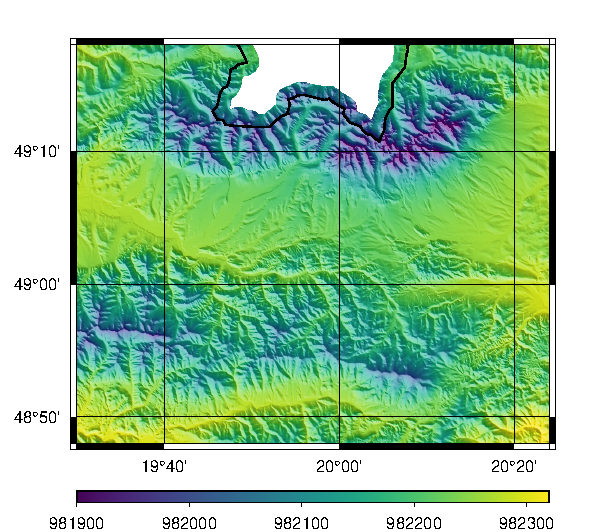
\includegraphics{./fig-gg-grav-sr-2arcsec.pdf}
\caption{Veľkosť gravitačného zrýchlenia~$\| \vec g_\gidx \|$ na zemskom 
povrchu v~oblasti Vysokých a~Nízkych Tatier (jednotky~mGal).  Dáta sú prevzaté 
z~modelu \texttt{grav-sr-2arcsec} \parencite{GravSR2arcsec}.}
\label{fig:gg_grav_sr_2arcsec}
\end{figure}

\begin{figure}
\centering
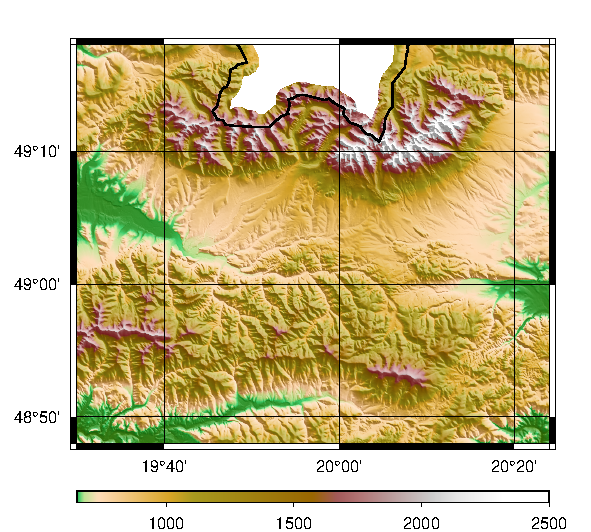
\includegraphics{./fig-h-grav-sr-2arcsec.pdf}
\caption{Topografia v~oblasti Vysokých a~Nízkych Tatier vyjadrená pomocou 
elipsoidickej výšky (jednotky~m).  Dáta sú prevzaté z~modelu 
\texttt{grav-sr-2arcsec} \parencite{GravSR2arcsec}.}
\label{fig:h_grav_sr_2arcsec}
\end{figure}







\subsection{Gravitačný potenciál}
\label{sec:vg}

Gravitačné zrýchlenie je vektorová veličina, ktorá je v~každom bode definovaná 
trojicou reálnych čísel.  V~niektorých situáciách je výhodnejšie pracovať so 
skalárnou veličinou, teda takou, ktorá je v~každom bode definovaná práve jedným 
reálnym číslom.  Tento prístup je mladší ako Newtonov gravitačný zákon zhruba 
o~jedno storočie \parencite{MacMillan1930,Jekeli2015}.  Fenomén gravitácie 
chápe ako \emph{pole}, ktorého vlastnosti môžu byť popísané rôznymi vzájomne 
súvisiacimi veličinami.  Podľa \textcite{MacMillan1930} prišiel s~konceptom 
potenciálu poľa taliansky matematik a~astronóm J.~L.~Lagrange~(1736--1813).  Ak 
by sme našli skalárnu veličinu gravitačného poľa, informáciu poskytnutú troma 
číslami v~podobe gravitačného vektora by sme dokázali zredukovať na jedno 
jediné číslo bez straty informácie o~poli samotnom.  Skalárna veličina 
gravitačného poľa sa nazýva \emph{gravitačný potenciál} a~označuje sa 
symbolom~$V_\gidx$.

Gravitačný potenciál definujeme pomocou gravitačného zrýchlenia.  Pre 
pochopenie vzťahu medzi oboma veličinami najprv predstavíme diferenciálny 
operátor gradient a~následne pristúpime k~samotnej definícii gravitačného 
potenciálu.

\subsubsection{Operátor gradient v~karteziánskom súradnicovom systéme}
\label{sec:gradient}

Nech~$x, y, z$ je trojrozmerný karteziánsky súradnicový systém s~jednotkovými 
vektormi~$\vec e_1, \vec e_2, \vec e_3$, ktoré sú rovnobežné so smerom 
súradnicových osí (Obrázok~\ref{fig:3d_coord_system}),
%
\begin{equation}
\label{eq:unit_vectors}
\vec e_1 =
\begin{bmatrix}
1\\
0\\
0\\
\end{bmatrix}
{,} \quad
%
\vec e_2 =
\begin{bmatrix}
0\\
1\\
0
\end{bmatrix}
%
{,}\quad
%
\vec e_3 =
\begin{bmatrix}
0\\
0\\
1
\end{bmatrix}
{,}
\end{equation}
%
\begin{equation}
\label{eq:unit_vectors_unit_length}
\| \vec e_i \| = 1{,} \quad i = 1, 2,3{.}
\end{equation}
%
Gradient skalárnej diferencovateľnej funkcie~$f(x, y, z)$ je vektorová 
funkcia~$\vec f(x, y, z)$, ktorá udáva \emph{smer a~veľkosť najväčšieho 
nárastu} funkcie~$f$ v~bode so súradnicami~$x, y, z$.  V~trojrozmernom 
karteziánskom súradnicovom systéme~$x, y, z$ je gradient funkcie~$f$ daný 
predpisom
%
\begin{equation}
\label{eq:gradient}
\vec f = \nabla f = \grad \ f = \vec e_1 \, \frac{\partial f}{\partial x} 
+ \vec e_2 \, \frac{\partial
f}{\partial y} + \vec e_3 \, \frac{\partial f}{\partial z} =
\begin{bmatrix}
\dfrac{\partial f}{\partial x}\\[2ex]
\dfrac{\partial f}{\partial y}\\[2ex]
\dfrac{\partial f}{\partial z}
\end{bmatrix}
{.}
\end{equation}
%
Symbol~$\nabla$, resp.~$\grad$ označuje operátor gradient.  Zložky 
vektora~$\vec f(x, y, z)$ teda vyjadrujú zmenu skalárnej funkcie~$f$ v~bode~$x, 
y, z$ v~smere vektorov~$\vec e_1, \vec e_2, \vec e_3$.

Operátor gradient je \emph{lineárny}, teda pre diferencovateľné funkcie~$f$ 
a~$g$ a~konštantu~$c$ platí
%
\begin{align}
\label{eq:gradient_additivity}
\nabla \left(f + g \right) &= \nabla f + \nabla g{,}\\
%
\label{eq:gradient_homogenity}
\nabla (c \, f) &= c \, \nabla f{.}
\end{align}

Numerická ukážka aplikácie operátora gradient je uvedená 
v~Prílohe~\ref{app:numerical_application_of_gradient}.

\begin{figure}
\centering
\input{./fig-3d-coord-system.pdf_tex}
\caption{Trojrozmerný karteziánsky súradnicový systém a~jednotkové vektory.}
\label{fig:3d_coord_system}
\end{figure}

\subsubsection{Definícia gravitačného potenciálu}

Gravitačný potenciál je skalárna funkcia, ktorá vyhovuje rovnici 
\parencite{SansoGeoidDetermination}
%
\begin{equation}
\label{eq:gg_grad_vg}
\vec g_\gidx(P) = \nabla V_\gidx(P)
\end{equation}
%
a~spĺňa podmienku
%
\begin{equation}
\label{eq:vg_at_infty}
\lim_{P \to \infty} V_\gidx(P) = 0{.}
\end{equation}
%
Vzťah~(\ref{eq:gg_grad_vg}) hovorí, že vektor~$\vec g_\gidx(P)$ udáva smer 
a~veľkosť najväčšieho nárastu gravitačného potenciálu v~bode~$P$.  
Rovnica~(\ref{eq:vg_at_infty}) znamená, že v~nekonečnej vzdialenosti od telesa 
nadobúda gravitačný potenciál nulovú hodnotu.  Tento vzťah zabezpečuje, že 
existuje práve jedna funkcia~$V_\gidx$, ktorá vyhovuje 
rovnici~(\ref{eq:gg_grad_vg}) \parencite{SansoGeoidDetermination}.

Poznamenajme, že bod s~nulovým gravitačným potenciálom je možné vybrať 
ľubovoľne, čo však neznamená, že jeho voľba je nedôležitá.  Naopak, miesto 
nulového gravitačného potenciálu ovplyvňuje hodnoty gravitačného potenciálu.  
Gravitačný potenciál je teda \emph{relatívna} veličina.  Často je preto 
dôležitejšie poznať relatívne vzťahy medzi gravitačným potenciálom v~priestore, 
napríklad rozdiel potenciálu medzi dvoma bodmi, než je potrebné poznať 
absolútnu hodnotu gravitačného potenciálu v~niektorom bode.

Gravitačný potenciál hmotného bodu s~hmotnosťou~$m$ je daný vzťahom
%
\begin{equation}
\label{eq:vg_point_mass}
V_\gidx(P) = \frac{G \, m}{\ell}{.}
\end{equation}
%
Overme, či tento vzťah vyhovuje rovniciam~(\ref{eq:gg_grad_vg}) 
a~(\ref{eq:vg_at_infty}).  Aplikujme operátor gradient 
z~rovnice~(\ref{eq:gradient}) na gravitačný potenciál~(\ref{eq:vg_point_mass}).  
S~využitím rovníc~(\ref{eq:r}) a~(\ref{eq:l}) dostaneme vzťah
%
\begin{equation}
\label{eq:gg_from_vg_point_mass}
\nabla V_\gidx(P) = \nabla \left( \frac{G \, m}{\ell} \right) = G \, m \, 
\nabla \left( \frac{1}{\ell} \right) =
%
G \, m
%
\begin{bmatrix}
\dfrac{\partial}{\partial x} \left( \dfrac{1}{\ell} \right)\\[2ex]
\dfrac{\partial}{\partial y} \left( \dfrac{1}{\ell} \right)\\[2ex]
\dfrac{\partial}{\partial z} \left( \dfrac{1}{\ell} \right)
\end{bmatrix}
%
=
%
-G \, m
%
\begin{bmatrix}
\dfrac{x - x'}{\ell^3}{,}\\[2ex]
\dfrac{y - y'}{\ell^3}{,}\\[2ex]
\dfrac{z - z'}{\ell^3}
\end{bmatrix}
%
=
%
-G \, \frac{m}{\ell^3} \, \vec{r}{.}
\end{equation}
%
Využili sme pritom vlastnosť operátora gradient~(\ref{eq:gradient_homogenity}), 
pretože $G \, m$ z~rovnice~(\ref{eq:vg_point_mass}) je konštanta.  
Vzťah~(\ref{eq:gg_from_vg_point_mass}) predstavuje gravitačné zrýchlenie~$\vec 
g_\gidx(P)$ z~rovnice~(\ref{eq:gg_point_mass}), čím bola dokázaná 
rovnosť~(\ref{eq:gg_grad_vg}).  Platnosť vzťahu~(\ref{eq:vg_at_infty}) pre 
$V_\gidx$ z~rovnice~(\ref{eq:vg_point_mass}) je zrejmá,
%
\begin{equation}
\lim_{\ell \to \infty} \frac{G \, m}{\ell} = 0{.}
\end{equation}

V~sústave~$N$ hmotných bodov získame celkový gravitačný potenciál opäť 
princípom superpozície, teda súčtom čiastkových gravitačných príspevkov 
jednotlivých hmotných bodov,
%
\begin{equation}
\label{eq:vg_N_point_masses}
V_\gidx(P) = \sum_{i = 1}^{N} V_{\gidx,i}(P) = G \sum_{i = 1}^{N}\frac{
m_i}{\ell_i}{.}
\end{equation}
%
Podobným spôsobom ako v~rovnici~(\ref{eq:gg_from_vg_point_mass}) sa môžeme 
presvedčiť, že aplikovaním operátora gradient na gravitačný 
potenciál~(\ref{eq:vg_N_point_masses}) získame gravitačné 
zrýchlenie~(\ref{eq:gg_N_point_masses}).  Rovnice~(\ref{eq:gg_grad_vg}) 
a~(\ref{eq:vg_at_infty}) teda platia i~v~prípade gravitačného potenciálu, ktorý 
je generovaný sústavou~$N$ hmotných bodov.

Od gravitačného potenciálu~$N$ hmotných bodov prejdeme ku
gravitačnému potenciálu všeobecného telesa podobnou úvahou ako
v~Kapitole~\ref{sec:gg}.  Teleso rozdelíme na diferenciálne hmotné elementy
$\diff m = \rho \, \diff \tau$ a~gravitačný potenciál získame integráciou,
%
\begin{equation}
\label{eq:vg_body}
V_\gidx(P) = G \iiint\limits_{\tau} \frac{\rho}{\ell} \, \diff\tau{.}
\end{equation}
%
Dôkaz, že rovnica~(\ref{eq:vg_body}) vyhovuje prijatej definícii gravitačného
potenciálu (rovnice~\ref{eq:gg_grad_vg} a~\ref{eq:vg_at_infty}) vynecháme, no 
je
dostupný napríklad v~\textcite{MacMillan1930}.

K~definícii a~interpretácii gravitačného potenciálu je možné pristúpiť aj 
z~fyzikálneho hľadiska.  Bez podrobného odvodenia sa obmedzíme na tvrdenie, že 
hodnota gravitačného potenciálu v~bode~$P$ predstavuje prácu, ktorú musí 
vykonať gravitačné pole pri premiestnení hmotného bodu s~hmotnosťou~$1\ 
\mathrm{kg}$ z~miesta s~nulovým potenciálom (v geodézii nekonečno, pozri 
vzťah~\ref{eq:vg_at_infty}) do bodu~$P$ 
\parencite{MacMillan1930,Kellogg1967,TorgeGeodesy}.  \emph{Práca} je dráhový 
účinok sily, v~tomto prípade gravitačnej.  Gravitačná sila má tú vlastnosť, že 
práca spôsobená jej silovým účinkom \emph{nezávisí} od dráhy, dôležitý je iba 
začiatočný a~koncový bod dráhy.  Ak sú začiatočný a~koncový bod totožné, práca 
je nulová.  Bez tejto vlastnosti by nebolo možné nájsť skalárnu funkciu 
$V_\gidx$, ktorá by vyhovovala rovnici~(\ref{eq:gg_grad_vg}).

Na rozdiel od gravitačného zrýchlenia, gravitačný potenciál nedokážeme
priamo merať.  Vo fyzikálnej geodézii často vystupuje ako neznáma funkcia,
ktorú sa snažíme určiť, napríklad z~gravitačného zrýchlenia.  Gravitačný 
potenciál má v~sústave~SI fyzikálnu jednotku~$\mathrm{m}^2\ \mathrm{s}^{-2}$.
Obrázok~\ref{fig:vg_grav_sr_2arcsec} znázorňuje gravitačný potenciál v~oblasti 
Vysokých a~Nízkych Tatier.

\begin{figure}
\centering
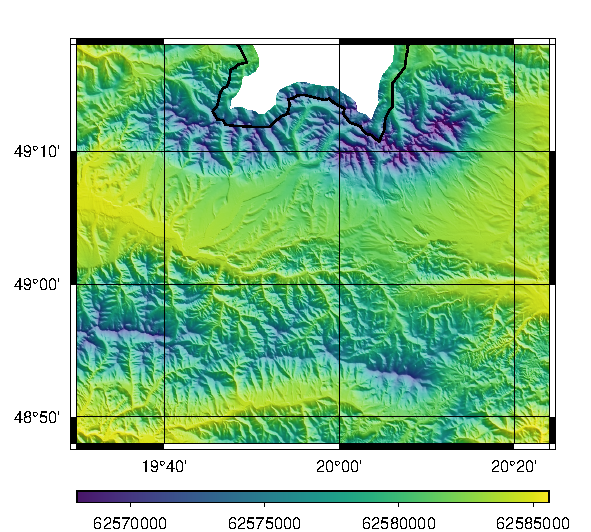
\includegraphics{./fig-vg-grav-sr-2arcsec.pdf}
\caption{Gravitačný potenciál~$V_\gidx$ na zemskom povrchu v~oblasti Vysokých
a~Nízkych Tatier (jednotky~$\mathrm{m}^2 \ \mathrm{s}^{-2}$).  Dáta sú prevzaté
z~modelu \texttt{grav-sr-2arcsec} \parencite{GravSR2arcsec}.}
\label{fig:vg_grav_sr_2arcsec}
\end{figure}






\section{Teória potenciálu}
\label{sec:potential_theory}

Rovnica~(\ref{eq:vg_body}) sa v~geovedách zvykne nazývať \emph{Newtonov
integrál}.  Hovorí, že gravitačný potenciál telesa môže byť vypočítaný, ak 
poznáme tvar telesa a~priestorové rozloženie hustoty v~jeho vnútri.  Newtonov
integrál má vo fyzikálnej geodézii kľúčový význam, nakoľko gravitačný potenciál 
obsahuje informáciu o~všetkých veličinách gravitačného poľa.

Newtonov integrál položil základy novej oblasti matematiky a~matematickej 
fyziky s~názvom \emph{teória potenciálu}.  Podľa \textcite{MacMillan1930} 
siahajú jej začiatky k~francúzskemu matematikovi, fyzikovi, astronómovi 
a~politikovi P.~S.~Laplaceovi (1749--1827).  Ten si uvedomil, že gravitačný 
potenciál každého všeobecného telesa má spoločné určité vlastnosti, čím vzniká 
zaujímavá množina funkcií hodná podrobnejšieho štúdia.  Významnosť teórie 
potenciálu iba potvrdzuje skutočnosť, ktorá je známa približne od čias 
C.~F.~Gaussa, a~síce že túto teóriu je možné aplikovať nielen na gravitačné 
pole, ale napríklad aj na magnetické či elektrostatické pole (spomeňme si na 
Coulombov zákon a~porovnajme ho s~Newtonovým gravitačným 
zákonom~\ref{eq:newton_law}).  Teória potenciálu teda študuje 
vzťah~(\ref{eq:vg_body}) vo všeobecnom zmysle, zaoberá sa rozličnými zdrojmi 
poľa (hmotný bod, hmotná priamka, nekonečne tenká vrstva, všeobecné teleso 
a~pod.) s~rôznym priestorovým rozložením hustôt (napríklad konštantná, 
premenlivá či dokonca i~záporná) a~neobmedzuje sa iba na gravitačné pole.  Táto 
úloha je nesmierne náročná.  Čo sa napríklad stane, ak sa 
v~rovniciach~(\ref{eq:gg_body}) a~(\ref{eq:vg_body}) nachádza výpočtový bod~$P$ 
vo vnútri telesa?  Za takýchto okolností musí nevyhnutne dôjsť k~situácii, 
v~ktorej sú súradnice bodu~$P$ identické so súradnicami jedného diferenciálneho 
hmotného elementu~$\diff m$.  Vzájomná vzdialenosť medzi bodom~$P$ 
a~elementom~$\diff m$, ktorá vystupuje v~menovateli, bude preto~$\ell = 0$.  
Konvergujú alebo divergujú v~takomto prípade integrály~(\ref{eq:gg_body}) 
a~(\ref{eq:vg_body})?  Jednou z~mnohých ďalších výziev sú gravitačné polia 
generované objektmi komplikovaných tvarov, napríklad Zemou, ktorej povrch 
obsahuje ostré hrany.  Je preto prirodzené, že teória potenciálu pritiahla 
záujem brilantných matematikov akými boli, okrem iných, J.~L.~Lagrange, 
A.--M.~Legendre (1752~-- 1833), P.~S.~Laplace, britský samouk G.~Green 
(1793--1841) či C.~F.~Gauss (pre diskusiu o~Gaussovom prínose pozri napríklad 
\cite{Freeden2018}).

V~nasledujúcich šiestich kapitolách (\ref{sec:regular_function}~až 
\ref{sec:poisson_equation}) sa budeme zaoberať niektorými základnými
vlastnosťami gravitačného potenciálu, ktoré vyplývajú z~teórie potenciálu.






\subsection{Podmienka regularity}
\label{sec:regular_function}

Gravitačný potenciál hmotného bodu a~gravitačný potenciál všeobecného telesa sú 
regulárne funkcie v~nekonečne.  Funkcia~$U$ je \emph{regulárna v~nekonečne}, ak 
platí \parencite{Kellogg1967,Pick1973}
%
\begin{equation}
\label{eq:regular_function}
\lim_{\ell \rightarrow \infty}\left| \ell \, U \right| < C{,} \quad \lim_{\ell 
\rightarrow \infty}\left| \ell^2 \, \frac{\partial U}{\partial x} \right| 
< C{,} \quad \lim_{\ell \rightarrow \infty}\left| \ell^2 \, \frac{\partial 
U}{\partial y} \right| < C{,} \quad \lim_{\ell \rightarrow \infty}\left| \ell^2 
\, \frac{\partial U}{\partial z} \right| < C{,}
\end{equation}
%
kde~$\ell$ je vzdialenosť od ľubovoľného pevného bodu a~$C$ je konštanta.

V~tejto práci sa obmedzíme iba na dôkaz, že prvá 
limita~(\ref{eq:regular_function}) pre gravitačný potenciál hmotného 
bodu~(\ref{eq:vg_point_mass}) je konečná.  Vzdialenosť~$\ell$ 
v~nerovnostiach~(\ref{eq:regular_function}) môže byť uvažovaná od ľubovoľného 
pevného bodu v~priestore.  Ak za tento pevný bod zvolíme polohu hmotného bodu 
s~hmotnosťou~$m$, potom~$\ell$ v~rovnici~(\ref{eq:vg_point_mass}) 
a~v~nerovnostiach~(\ref{eq:regular_function}) predstavuje tú istú vzdialenosť, 
teda
%
\begin{equation}
\lim_{\ell \rightarrow \infty} \left| \ell \, V_\gidx \right| = \lim_{\ell 
\rightarrow \infty} \left| \ell \, \frac{G \, m}{\ell} \right| = \lim_{\ell 
\rightarrow \infty} \left| G \, m \right| = G \, m{.}
\end{equation}

Pre gravitačný potenciál všeobecného telesa~(\ref{eq:vg_body}) uvedieme bez 
dôkazu nasledovnú rovnosť,
%
\begin{equation}
\label{eq:vg_regular}
\lim_{\ell \rightarrow \infty} \left| \ell \, V_\gidx \right| = G \, M{,}
\end{equation}
%
kde~$M$ je hmotnosť všeobecného telesa.  Pre dôkaz, že gravitačný potenciál 
všeobecného telesa~(\ref{eq:vg_body}) vyhovuje 
nerovnostiam~(\ref{eq:regular_function}) pozri napríklad~\textcite{Pick1973}.





\subsection{Laplaceova rovnica v~karteziánskych súradniciach}
\label{sec:laplace_equation_cart}

Pierre-Simon Laplace zistil, že gravitačný potenciál každého všeobecného telesa
spĺňa v~priestore \emph{mimo} hmôt rovnicu
%
\begin{equation}
\label{eq:vg_laplace_cart}
\nabla^2 V_\gidx = \Delta V_\gidx = \frac{\partial^2 V_\gidx}{\partial x^2}
+ \frac{\partial^2 V_\gidx}{\partial y^2} + \frac{\partial^2 V_\gidx}{\partial
z^2} = 0{.}
\end{equation}
%
Operátor~$\nabla^2 = \Delta$ sa nazýva \emph{Laplaceov operátor} 
a rovnica~(\ref{eq:vg_laplace_cart}) sa nazýva \emph{Laplaceova rovnica} pre
gravitačný potenciál.

Aplikáciu Laplaceovho operátora na dvakrát diferencovateľnú funkciu~$f$ môžeme 
zapísať pomocou už známeho operátora gradient~(\ref{eq:gradient}) 
\parencite{SansoGeoidDetermination},
%
\begin{equation}
\label{eq:laplace_cart_grad_grad_notation}
\begin{split}
\nabla^2 f &= \nabla \cdot \left( \nabla f \right) = \left( \vec e_1 \, 
\frac{\partial}{\partial x} + \vec e_2 \, \frac{\partial}{\partial y} + \vec 
e_3 \, \frac{\partial}{\partial z} \right) \cdot \left( \vec e_1 \, 
\frac{\partial f}{\partial x} + \vec e_2 \, \frac{\partial f}{\partial y} 
+ \vec e_3 \, \frac{\partial f}{\partial z} \right)\\
%
&= \vec e_1 \cdot \frac{\partial \vec e_1}{\partial x} \, \frac{\partial 
f}{\partial x} + \vec e_1 \cdot \vec e_1 \frac{\partial^2 f}{\partial x^2} 
+ \vec e_1 \cdot \frac{\partial \vec e_2}{\partial x} \, \frac{\partial 
f}{\partial y} + \vec e_1 \cdot \vec e_2 \frac{\partial^2 f}{\partial x \, 
\partial y} + \dots + \vec e_3 \cdot \vec e_3 \frac{\partial^2 f}{\partial 
z^2}\\
%
&=\frac{\partial^2 f}{\partial x^2} + \frac{\partial^2 f}{\partial y^2} 
+ \frac{\partial^2 f}{\partial z^2}{,}
\end{split}
\end{equation}
%
kde symbol $\cdot$ označuje \emph{skalárny súčin dvoch vektorov}.\footnote{Oblé 
zátvorky v~rovnici~(\ref{eq:laplace_cart_grad_grad_notation}) sú použité na 
určenie priority algebrických operácií násobenia a~sčítania, nie na označenie 
prvkov vektorov.  Prvky vektorov a~matíc udávame vždy v~hranatých zátvorkách.} 
Na získanie posledného výrazu 
v~rovnici~(\ref{eq:laplace_cart_grad_grad_notation}) sme využili nasledovné 
vlastnosti jednotkových vektorov a~skalárneho súčinu vektorov,
%
\begin{align}
\label{eq:ei_orthogonality}
\vec e_i \cdot \vec e_j &= \| \vec e_i \| \, \| \vec e_j \| \, \cos(90^\circ) 
= 0{,} \quad i \neq j{,}\\
%
\label{eq:ei_unit_length}
\vec e_i \cdot \vec e_i &= \| \vec e_i \| \, \| \vec e_i \| \, \cos(0^\circ) 
= 1{,}\\
%
\label{eq:ei_derivatives}
\frac{\partial \vec e_i}{\partial x} &= \frac{\partial \vec e_i}{\partial y} 
= \frac{\partial \vec e_i}{\partial z} = \vec 0{.}
\end{align}
%
Rovnica~(\ref{eq:ei_orthogonality}) vyplýva z~\emph{ortogonálnosti} 
jednotkových vektorov~$\vec e_i$ a~$\vec e_j$ pre~$i \neq j$ (pozri 
Obrázok~\ref{fig:3d_coord_system}).  Rovnica~(\ref{eq:ei_unit_length}) je 
dôsledkom vzťahu~(\ref{eq:unit_vectors_unit_length}).  
Vzťahy~(\ref{eq:ei_derivatives}) vyplývajú z~definície jednotkových 
vektorov~(\ref{eq:unit_vectors}).

Laplaceov operátor je \emph{lineárny}, teda pre dvakrát diferencovateľné 
funkcie $f$ a~$g$ a~konštantu~$c$ platí
%
\begin{align}
\label{eq:laplace_additivity}
\nabla^2 \left(f + g \right) &= \nabla^2 f + \nabla^2 g{,}\\
%
\label{eq:laplace_homogenity}
\nabla^2 (c \, f) &= c \, \nabla^2 f{.}
\end{align}

Overme, či gravitačný potenciál hmotného bodu~(\ref{eq:vg_point_mass}) vyhovuje 
Laplaceovej rovnici~(\ref{eq:vg_laplace_cart}).  Budeme uvažovať 
vzdialenosť~$\ell > 0$, pretože gravitačný potenciál hmotného bodu nie je 
definovaný pre~$\ell = 0$.  S~využitím~(\ref{eq:vg_point_mass}) 
a~(\ref{eq:laplace_homogenity}) dostaneme vzťah
%
\begin{equation}
\nabla^2 V_\gidx = \nabla^2 \left( \frac{G \, m}{\ell} \right) = G \, m \, 
\nabla^2 \left( \frac{1}{\ell} \right){,}
\end{equation}
%
keďže~$G \, m$ je konštanta.  Postačuje preto dokázať rovnosť
%
\begin{equation}
\label{eq:nabla_l}
\nabla^2 \left( \frac{1}{\ell} \right) = \frac{\partial^2}{\partial x^2}\left( 
\frac{1}{\ell} \right) + \frac{\partial^2}{\partial y^2}\left( \frac{1}{\ell} 
\right) + \frac{\partial^2}{\partial z^2}\left( \frac{1}{\ell} \right) = 0{.}
\end{equation}
%
Vypočítajme druhé parciálne derivácie funkcie~$1 \slash \ell$ v~smere 
súradnicových osí s~využitím rovnice~(\ref{eq:l}),
%
\begin{equation}
\label{eq:l_2nd_derivatives}
\begin{split}
\frac{\partial^2}{\partial x^2} \left( \frac{1}{\ell} \right) &=
\frac{\partial}{\partial x} \left( -\frac{x - x'}{\ell^3} \right) = \left(3
\frac{(x - x')^2}{\ell^5} - \frac{1}{\ell^3} \right){,}\\
%
\frac{\partial^2}{\partial y^2} \left( \frac{1}{\ell} \right) &=
\frac{\partial}{\partial y} \left( -\frac{y - y'}{\ell^3} \right) = \left(3
\frac{(y - y')^2}{\ell^5} - \frac{1}{\ell^3} \right){,}\\
%
\frac{\partial^2}{\partial z^2} \left( \frac{1}{\ell} \right) &=
\frac{\partial}{\partial z} \left( -\frac{z - z'}{\ell^3} \right) = \left(3
\frac{(z - z')^2}{\ell^5} - \frac{1}{\ell^3} \right){.}
\end{split}
\end{equation}
%
Súčet členov na pravej strane rovníc~(\ref{eq:l_2nd_derivatives}) je nulový, čo 
dokazuje rovnosť~(\ref{eq:nabla_l}).  Gravitačný potenciál hmotného 
bodu~(\ref{eq:vg_point_mass}) teda vyhovuje Laplaceovej diferenciálnej 
rovnici~(\ref{eq:vg_laplace_cart}) pre~$\ell > 0$.

Pomocou vzťahov~(\ref{eq:vg_N_point_masses}), (\ref{eq:laplace_additivity}), 
(\ref{eq:laplace_homogenity}) a~(\ref{eq:l_2nd_derivatives}) je možné 
presvedčiť sa, že Laplaceovej rovnici vyhovuje i~gravitačný potenciál, ktorý je 
generovaný sústavou~$N$ hmotných bodov,
%
\begin{equation}
\label{eq:gg_N_point_masses_laplace}
\nabla^2 \left( \sum_{i = 1}^N V_{\gidx,i} \right) = \sum_{i = 1}^N \nabla^2
V_{\gidx,i} = G \, \sum_{i = 1}^N m_i \nabla^2 \left( \frac{1}{\ell_i} \right) 
= 0{.}
\end{equation}
%
Rovnica~(\ref{eq:gg_N_point_masses_laplace}) platí opäť iba za predpokladu, 
že~$\ell_i > 0$ pre~$i = 1, 2, \dots, N$.  Táto podmienka je splnená, ak poloha 
bodu, v~ktorom je Laplaceova rovnica počítaná, je rozdielna od polôh 
všetkých~$N$ hmotných bodov.

Podobne je možné ukázať, že Laplaceova rovnica pre gravitačný potenciál 
všeobecného telesa platí vo všetkých bodoch \emph{mimo} telesa,
%
\begin{equation}
\nabla^2 V_\gidx = G\, \iiint\limits_\tau \rho \, \left[ 
\frac{\partial^2}{\partial
x^2}\left(\frac{1}{\ell}\right) + \frac{\partial^2}{\partial
y^2}\left(\frac{1}{\ell}\right) + \frac{\partial^2}{\partial
z^2}\left(\frac{1}{\ell}\right) \right] \diff\tau = 0{.}
\end{equation}


\subsection{Laplaceova rovnica vo sférických súradniciach}
\label{sec:laplace_equation_sph}

Kvôli približne sférickému tvaru Zeme je často výhodnejšie popisovať zemské 
gravitačné pole v~krivočiarych sférických súradniciach než v~karteziánskych 
súradniciach.  Je preto potrebné nájsť tvar operátora gradient 
(rovnica~\ref{eq:gradient}) a~Laplaceovho operátora 
(rovnica~\ref{eq:laplace_cart_grad_grad_notation}) aj vo sférických 
súradniciach.  Zaujímavosťou je, že Laplace v~skutočnosti prvýkrát publikoval 
rovnicu~(\ref{eq:vg_laplace_cart}) práve v~krivočiarych sférických 
súradniciach, a~nie v~karteziánskych súradniciach \parencite{MacMillan1930}.

Sférické súradnice budeme označovať symbolmi~$r, \varphi, \lambda$, pričom~$r$ 
predstavuje sprievodič, $\varphi$ je sférická šírka a~$\lambda$ je sférická 
dĺžka (Obrázok~\ref{fig:cart_sph}).  Medzi sférickými a~karteziánskym 
súradnicami platia vzťahy (pozri Obrázok~\ref{fig:cart_sph})
%
\begin{equation}
\label{eq:sph2cart}
\begin{split}
x &= r \, \cos\varphi \, \cos\lambda{,}\\
y &= r \, \cos\varphi \, \sin\lambda{,}\\
z &= r \, \sin\varphi\\
\end{split}
\end{equation}
%
a
%
\begin{equation}
\label{eq:cart2sph}
\begin{split}
r &= \sqrt{x^2 + y^2 + z^2}{,}\\
\varphi &= \arctan \frac{z}{\sqrt{x^2 + y^2}}{,}\\
\lambda &= \arctan \frac{y}{x}{.}\\
\end{split}
\end{equation}

\begin{figure}
\centering
\input{./fig-cart-sph.pdf_tex}
\caption{Karteziánske súradnice~$x, y, z$ a~sférické súradnice~$r, \varphi, 
\lambda$ bodu~$P$.  Symboly~$\vec{e}_1^\mathrm{s}, \vec{e}_2^\mathrm{s}, 
\vec{e}_3^\mathrm{s}$ označujú jednotkové vektory lokálneho karteziánskeho 
súradnicového systému~$x^\mathrm{s}, y^\mathrm{s}, z^\mathrm{s}$ s~pohyblivým 
začiatkom v~bode~$P$.}
\label{fig:cart_sph}
\end{figure}

Operátor gradient má vo sférických súradniciach tvar (pozri 
Prílohu~\ref{app:gradient_in_orthogonal_systems})
%
\begin{equation}
\label{eq:gradient_sph}
\nabla f = \grad f = \vec e_1^\mathrm{s} \, \frac{1}{r} \, \frac{\partial 
f}{\partial \varphi} + \vec e_2^\mathrm{s} \, \frac{1}{r \, \cos\varphi} \, 
\frac{\partial f}{\partial \lambda} + \vec e_3^\mathrm{s} \, \frac{\partial 
f}{\partial r}\\
%
=
%
\begin{bmatrix}
\dfrac{1}{r} \, \dfrac{\partial f}{\partial \varphi} \\[2ex]
\dfrac{1}{r \, \cos\varphi} \, \dfrac{\partial f}{\partial \lambda}\\[2ex]
\dfrac{\partial f}{\partial r}
\end{bmatrix}
{.}
\end{equation}
%
Symboly~$\vec{e}_1^\mathrm{s}, \vec{e}_2^{\mathrm{s}}, \vec{e}_3^\mathrm{s}$ 
označujú jednotkové vektory súradnicových osí~$x^\mathrm{s}, y^\mathrm{s}, 
z^\mathrm{s}$ lokálneho karteziánskeho súradnicového systému orientovaného na 
sever s~pohyblivým začiatkom v~bode~$P$~(Obrázok~\ref{fig:cart_sph}).  
Os~$z^\mathrm{s}$ je daná smerom sprievodiča prechádzajúceho bodom~$P$ a~je 
orientovaná kladne vo vonkajšom smere.  Os~$x^\mathrm{s}$ leží v~rovine 
meridiánu a~je orientovaná kladne na sever.  Os~$y^\mathrm{s}$ dotvára 
pravouhlý \emph{ľavotočivý} súradnicový systém.  Aplikovaním operátora 
gradient~(\ref{eq:gradient_sph}) na gravitačný potenciál~$V_\gidx(r, \varphi, 
\lambda)$ získame gravitačné zrýchlenie~$\vec g_\gidx(r, \varphi, \lambda)$, 
ktorého prvky popisujú zmenu gravitačného potenciálu v~bode~$P$ v~smere 
súradnicových osí~$x^\mathrm{s}, y^\mathrm{s}, z^\mathrm{s}$.

Laplaceova rovnica pre gravitačný potenciál má vo sférických súradniciach tvar 
(Príloha~\ref{app:laplace_in_spherical_coordinates})
%
\begin{equation}
\label{eq:vg_laplace_sph}
\nabla^2 V_\gidx = \frac{1}{r^2} \frac{\partial}{\partial r} \left( r^2 
\frac{\partial V_\gidx}{\partial r} \right) + \frac{1}{r^2 \, \cos\varphi} 
\frac{\partial}{\partial \varphi} \left( \cos\varphi \frac{\partial 
V_\gidx}{\partial \varphi} \right) + \frac{1}{r^2 \, 
\cos^2\varphi}\frac{\partial^2 V_\gidx}{\partial \lambda^2} = 0{.}
\end{equation}
%
Deriváciou oboch členov v~zátvorkách môžeme zapísať Laplaceovu rovnicu aj 
v~tvare
%
\begin{equation}
\label{eq:vg_laplace_sph2}
\nabla^2 V_\gidx = \frac{\partial^2 V_\gidx}{\partial r^2} + \frac{2}{r} \, 
\frac{\partial V_\gidx}{\partial r} + \frac{1}{r^2} \, \frac{\partial^2 
V_\gidx}{\partial \varphi^2} - \frac{\tan\varphi}{r^2} \, \frac{\partial 
V_\gidx}{\partial \varphi} + \frac{1}{r^2 \,
\cos^2\varphi}\frac{\partial^2 V_\gidx}{\partial \lambda^2} = 0{.}
\end{equation}
%
V~niektorých situáciách je výhodné vynásobiť ešte 
rovnicu~(\ref{eq:vg_laplace_sph2}) členom~$r^2$,
%
\begin{equation}
\label{eq:vg_laplace_sph3}
r^2 \, \frac{\partial^2 V_\gidx}{\partial r^2} + 2r \, \frac{\partial 
V_\gidx}{\partial r} + \frac{\partial^2 V_\gidx}{\partial \varphi^2} 
- \tan\varphi \, \frac{\partial V_\gidx}{\partial \varphi} 
+ \frac{1}{\cos^2\varphi}\frac{\partial^2 V_\gidx}{\partial \lambda^2} = 0{.}
\end{equation}



\subsection{Praktický význam Laplaceovej rovnice}
\label{sec:meaning_of_laplace_equation_in_practice}

Jedným z~cieľov fyzikálnej geodézie je určiť vonkajšie gravitačné pole Zeme 
z odmeraných veličín gravitačného poľa.  Z~praktických dôvodov je ale možné 
vykonávať merania iba v~malej časti priestoru mimo Zeme, napríklad 
v~bezprostrednej blízkosti zemského povrchu či na dráhe umelej družice Zeme.  
Preto ak chceme určiť gravitačné pole aj v~iných častiach priestoru mimo Zeme, 
bolo by vhodné porozumieť tomu, ako sa gravitačný potenciál v~tomto priestore 
mení.  Ak by nejaký princíp existoval a~bol by objavený, znamenalo by to, že 
hoci naše merania sú dostupné iba v~malej časti vonkajšieho priestoru Zeme, 
gravitačný potenciál mimo Zeme môže byť z~týchto meraní vypočítaný aj v~nových 
oblastiach, ktoré nie sú pokryté meraniami.

Tento princíp bol objavený a~je ním práve Laplaceova rovnica.  
V~Kapitole~\ref{sec:newton_law} sme ukázali, ako Newtonov gravitačný 
zákon~(\ref{eq:newton_law}) vysvetľuje \emph{princíp} (mechanizmus) pohybu 
planéty okolo Slnka.  Vďaka tomuto princípu postačuje poznať niekoľko vstupných 
údajov v~čase~$t_0$ (polohu planéty, vektor rýchlosti planéty a~vektor 
gravitačnej sily, ktorá pôsobí medzi Slnkom a~planétou) a~poloha planéty môže 
byť vypočítaná v~ľubovoľnom čase v~budúcnosti či v~minulosti.  Situácia je síce 
výrazne komplikovanejšia, ak uvážime prítomnosť ďalších nebeských telies, no aj 
táto úloha je riešiteľná v~princípe rovnakým spôsobom.  V~prípade Laplaceovej 
rovnice je situácia veľmi podobná.  Ak poznáme napríklad gravitačný potenciál 
či gravitačné zrýchlenie na celom povrchu Zeme a~ak poznáme aj tvar zemského 
povrchu, potom znalosť \emph{princípu} zmeny gravitačného 
potenciálu\footnote{Presnejšie by azda bolo hovoriť o~\textit{zmene zmeny} 
gravitačného potenciálu, keďže Laplaceova rovnica~(\ref{eq:vg_laplace_cart}) 
obsahuje druhé derivácie.} mimo Zeme v~podobe Laplaceovej rovnice umožňuje 
zistiť hodnotu gravitačného potenciálu v~ľubovoľnom bode tejto oblasti.  
Laplaceova rovnica má preto kľúčový význam pre určovanie vonkajšieho 
gravitačného poľa Zeme.  Dodajme, že Laplaceova rovnica platí mimo Zeme až po 
matematickom odstránení alebo zanedbaní hmôt zemskej atmosféry \parencite[pozri 
napríklad][]{Janak2006}.



\subsection{Harmonická funkcia}
\label{sec:harmonic_function}

Laplaceovej rovnici vyhovuje nielen gravitačný potenciál mimo telesa, ale
nekonečné množstvo funkcií.  Zaveďme preto pojem \emph{harmonická funkcia}.
Funkcia je harmonická v~oblasti~$\Omega$ trojrozmerného priestoru, ak vyhovuje 
Laplaceovej rovnici v~každom bode oblasti~$\Omega$ 
\parencite{MoritzPhysicalGeodesy}.  Ak oblasť~$\Omega$ je vonkajším priestorom 
uzavretej plochy, potom musí navyše spĺňať podmienku regularity 
\parencite[pozri 
nerovnosti~\ref{eq:regular_function};][]{MoritzPhysicalGeodesy}.

Harmonické funkcie majú niekoľko zaujímavých a~dôležitých vlastností 
\parencite[pozri napríklad][]{Kellogg1967,Pick1973,Janak2006}.  Na tomto mieste 
spomeňme aspoň jednu z~nich.  Každá harmonická funkcia je \emph{analytická} 
v~oblasti, v~ktorej vyhovuje Laplaceovej rovnici.  To znamená, že každá 
harmonická funkcia je spojitá, má spojité všetky derivácie a~v~okolí každého 
bodu oblasti~$\Omega$ ju možno rozvinúť do Taylorovho radu 
\parencite{MoritzPhysicalGeodesy}.  Táto vlastnosť je dôležitá, preto sa pri 
nej na chvíľku pristavme.

Nech~$f(x)$ je analytická funkcia, ktorá je nekonečne diferencovateľná 
v~bode~$x_0$.  \emph{Taylorov rozvoj} funkcie~$f(x)$ v~okolí bodu~$x_0$ má tvar
%
\begin{equation}
\label{eq:f_taylor}
f(x) = \sum_{n = 0}^\infty \frac{1}{n!} \, \left.\frac{\diff^n f(x)}{\diff x^n} 
\right|_{x = x_0} \, (x - x_0)^n{.}
\end{equation}
%
Zápis $\left.\frac{\diff^n f(x)}{\diff x^n} \right|_{x = x_0}$ označuje hodnotu 
$n$-tej derivácie funkcie~$f$ podľa~$x$ v~bode~$x_0$.  Pripomeňme, že~$0!  = 1$ 
a~ďalej že nultá derivácia funkcie~$f$ je rovná samotnej funkcii~$f$, 
teda~$\left.\frac{\diff^0 f(x)}{\diff x^0}\right|_{x = x_0} = f(x_0)$.

Uvažujme teraz všeobecné teleso.  Nech sú dané dva body,
$P_1(r, \varphi, \lambda)$ a~$P_2(r + \Delta r, \varphi, \lambda)$, $\Delta
r > 0$, nachádzajúce sa mimo tohto telesa a~na tej istej spojnici so začiatkom
súradnicového systému, ktorý sa nachádza v~ťažisku telesa
(Obrázok~\ref{fig:analytical_continuation}).  Keďže gravitačný potenciál je 
v~oblasti mimo hmôt harmonická, a~teda analytická funkcia, môžeme ho v~okolí 
bodu~$P_1$ rozvinúť do Taylorovho radu,
%
\begin{equation}
\label{eq:vg_analytical_continuation}
V_\gidx(P_2) = \sum_{n = 0}^\infty \frac{1}{n!} \, \left.\frac{\partial^n
V_\gidx}{\partial r^n}\right|_{P_1} \, \Delta r^n{.}
\end{equation}
%
Rovnica~(\ref{eq:vg_analytical_continuation}) hovorí, že z~lokálnych vlastností 
gravitačného potenciálu, ktoré sú obsiahnuté v~deriváciách~$\partial^n V_\gidx 
\slash \partial r^n$ v~bode~$P_1$, dokážeme určiť hodnotu gravitačného 
potenciálu v~ľubovoľnom bode v~radiálnom smere pre~$\Delta r > 0$.  Tento 
proces sa nazýva \emph{analytické pokračovanie} gravitačného potenciálu nahor.  
Čím je vzdialenosť~$\Delta r$ väčšia, tým pomalšie 
rad~(\ref{eq:vg_analytical_continuation}) spravidla konverguje a~naopak.  
Analyticky pokračovať je možné aj v~iných smeroch.  V~takom prípade je potrebné 
derivovať gravitačný potenciál v~príslušnom smere.  Rovnako tak je možné 
analyticky pokračovať aj iné veličiny gravitačného poľa, napríklad gravitačné 
zrýchlenie,
%
\begin{equation}
\label{eq:gg_analytical_continuation}
\vec g_\gidx(P_2) = \sum_{n = 0}^{\infty} \frac{1}{n!} \, 
\left.\frac{\partial^n \vec
g_\gidx}{\partial r^n}\right|_{P_1} \, \Delta r^n{.}
\end{equation}

\begin{figure}
\centering
\input{./fig-analytical-continuation.pdf_tex}
\caption{Analytické pokračovanie gravitačného poľa z~bodu~$P_1$ do bodu~$P_2$.}
\label{fig:analytical_continuation}
\end{figure}

Na záver dodajme, že situácia je výrazne komplikovanejšia, ak analyticky 
pokračujeme nadol z~bodu~$P_2$ do bodu~$P_1$.  Táto úloha je zle podmienená 
a numericky nestabilná \parencite{SansoGeodeticBoundaryValueProblem}.  
V~praktických aplikáciách to znamená, že i~malá zmena vo vstupných údajoch 
spôsobuje veľké zmeny vo výsledkoch.






\subsection{Poissonova rovnica}
\label{sec:poisson_equation}

Z~Kapitoly~\ref{sec:laplace_equation_cart} vieme, že Laplaceova rovnica pre
gravitačný potenciál platí v~každom bode mimo telesa.  \emph{Vo vnútri} telesa
platí \emph{Poissonova rovnica},
%
\begin{equation}
\label{eq:vg_poisson_equation}
\nabla^2 V_\gidx(P) = -4 \pi \, G \, \rho(P){,}
\end{equation}
%
kde~$\rho(P)$ je hustota v~bode~$P$.  Odvodenie Poissonovej rovnice je možné 
nájsť napríklad v~\textcite{MacMillan1930}, \textcite{Kellogg1967} či 
\textcite{SansoGeoidDetermination}.  Poissonovu rovnicu je možné vnímať ako 
zovšeobecnenie Laplaceovej rovnice.  Ak sa bod~$P$ vo 
vzťahu~(\ref{eq:vg_poisson_equation}) nachádza mimo hmôt, potom~$\rho(P) = 0$, 
čím dostávame Laplaceovu rovnicu~(\ref{eq:vg_laplace_cart}).  S.~D.~Poisson 
(1781~-- 1840) bol francúzsky matematik a~fyzik.  
Rovnicu~(\ref{eq:vg_poisson_equation}) publikoval v~roku 1813 v~práci 
\textit{Bulletin de la société philomatique}.

Posledná oblasť, v~ktorej sa môže bod~$P$ nachádzať, no nie je pokrytá ani 
Laplaceovou, ani Poissonovou rovnicou, je \emph{povrch} telesa.  Druhé 
derivácie gravitačného potenciálu vystupujúce v~operátore $\nabla^2$ (pozri 
rovnice~\ref{eq:vg_laplace_cart} a~\ref{eq:vg_laplace_sph}) nie sú vo 
všeobecnosti v~takom prípade definované \parencite{Kellogg1967}.  Dôvodom je 
nespojitosť hustoty~$\rho$, ktorá sa na povrchu telesa mení z~$\rho > 0$ na 0, 
resp. naopak, v~závislosti od smeru prechodu.






\section{Odstredivé pole a~tiažové pole}
\label{sec:centrifugal_gravity_field}

Newtonov gravitačný zákon~(\ref{eq:newton_law}) platí v~súradnicovom systéme,
ktorý je v~pokoji alebo je v~stave rovnomerného priamočiareho pohybu.  Takýto
súradnicový systém sa nazýva \emph{inerciálny súradnicový systém}.

Uvažujme trojrozmerný karteziánsky súradnicový systém so začiatkom v~ťažisku 
Zeme a~s~osou~$z$, ktorá je totožná s~rotačnou osou Zeme.  Os~$x$ nech leží 
v~priesečníku rovín rovníka a~Greenwichského meridiánu a~os~$y$ nech dotvára 
pravotočivý súradnicový systém.  Nech je tento súradnicový systém pevne spojený 
so Zemou.  Takýto súradnicový systém nie je inerciálny, pretože vzhľadom na 
inerciálny súradnicový systém v~ňom dochádza prinajmenšom k~dvom nelineárnym 
pohybom \parencite{SansoGeoidDetermination}.  Prvý vzniká v~dôsledku rotácie 
Zeme okolo vlastnej osi, druhý je spôsobený obehom Zeme okolo Slnka.  Aby sme 
mohli študovať sily pôsobiace na Zemi pomocou druhého Newtonovho pohybového 
zákona v~takomto neinerciálnom súradnicovom systéme, uvážiť musíme nielen 
gravitačnú silu, ale aj~ďalšie sily.  Na objekt, ktorý sa nachádza na rotujúcej 
Zemi, pôsobí okrem gravitačnej sily aj \emph{odstredivá sila}.  Ak je takýto 
objekt v~pohybe, pôsobí naň aj \emph{Coriolisova sila} 
\parencite{Torge1989,Jekeli2000,MoritzPhysicalGeodesy,SansoGeoidDetermination}.  
Azda väčšina geodetických meracích zariadení je počas merania vzhľadom k~Zemi 
v~pokoji, preto Coriolisovu silu nebudeme uvažovať.  Ak sa uhlová rýchlosť 
rotácie mení v~čase, je potrebné uvážiť~\emph{Eulerovu silu} 
\parencite{Torge1989,SansoGeoidDetermination}.  V~tejto práci predpokladáme, že 
uhlová rýchlosť rotácie Zeme je konštantná, preto nebudeme ďalej uvažovať ani 
Eulerovu silu.  Tieto tri sily, odstredivá, Coriolisova a~Eulerova, sa zaraďujú 
medzi \emph{zotrvačné sily}, niekedy tiež nazývané fiktívne sily.  Zotrvačné 
sily sú zdanlivé sily, ktoré sú spôsobené neinerciálnosťou vzťažnej sústavy 
pozorovateľa, a~teda nevznikajú vzájomným silovým pôsobením medzi objektmi.

Najvýznamnejšia zotrvačná sila vo fyzikálnej geodézii je spôsobená rotáciou 
Zeme a~nazýva sa \emph{odstredivá sila}
$\vec F_\cidx$.  Pole spôsobené rotáciou Zeme budeme nazývať \emph{odstredivé 
pole}.  Zatiaľ čo gravitačné pole Zeme je v~zmysle Newtonovho gravitačného 
zákona~(\ref{eq:newton_law}) dôsledkom hmôt, ktoré tvoria zemské teleso, 
odstredivé pole Zeme je spôsobené neinerciálnosťou vyššie opísaného 
súradnicového systému.  Uvážením spoločného pôsobenia gravitačného 
a~odstredivého poľa získame \emph{tiažové pole}.  Formálne teda môžeme napísať 
vzťah
%
\begin{equation*}
\textrm{Gravitačné pole} + \textrm{Odstredivé pole} = \textrm{Tiažové pole}{.}
\end{equation*}

Tiažové pole má pre fyzikálnu geodéziu fundamentálny význam.  Jedna z~veličín 
tiažového poľa, tiažové zrýchlenie, je totiž jedným z~prostredníkov, vďaka 
ktorým vieme získať a~matematicky uchopiť informáciu o~skutočnom tiažovom poli 
našej Zeme.  Ďalšia z~veličín tiažového poľa, tiažový potenciál, sa používa 
napríklad na definíciu fyzikálneho tvaru Zeme, teda geoidu (pozri úvodnú 
kapitolu).

V~nasledujúcich dvoch kapitolách popíšeme veličiny odstredivého a~tiažového 
poľa.






\subsection{Odstredivé a~tiažové zrýchlenie}
\label{sec:centrifugal_and_gravity_acceleration}

Uvažujme neinerciálny súradnicový systém~$x, y, z$ v~zmysle 
Kapitoly~\ref{sec:centrifugal_gravity_field}.  Odteraz však budeme navyše 
predpokladať, že uhlová rýchlosť rotácie Zeme~$\omega$ je konštantná a~tiež že 
rotačná os Zeme nemení svoju polohu voči súradnicovej osi~$z$.  Nech je daný 
hmotný bod~$P(x, y, z)$ s~hmotnosťou~$1\ \mathrm{kg}$ kdekoľvek na Zemi alebo 
v~jej vnútri.  V~dôsledku rotácie Zeme a~súradnicového systému, v~ktorom 
vyjadrujeme polohu, je hmotnému bodu~$P$ udeľované \emph{odstredivé 
zrýchlenie}~$\vec g_\cidx(P)$,
%
\begin{equation}
\label{eq:gc}
\vec g_\cidx(P) = \omega^2 \, \vec p =
%
\omega^2 \, \begin{bmatrix}
x\\
y\\
0
\end{bmatrix}
%
{.}
\end{equation}
%
Veľkosť odstredivého zrýchlenia~$\vec g_\cidx(P)$ sa mení iba so 
vzdialenosťou~$p = \| \vec p \|$ od rotačnej osi 
(Obrázok~\ref{fig:gravity_vector}),
%
\begin{equation}
\label{eq:gc_magnitude}
\| \vec g_\cidx \| = \omega^2 \, p = \omega^2 \, \sqrt{x^2 + y^2} = \omega^2 \, 
r \, \cos\varphi{.}
\end{equation}
%
Čím je vzdialenosť~$p$ väčšia, tým je väčšie i~odstredivé zrýchlenie a~naopak.
Smer vektora~$\vec g_\cidx(P)$ je kolmý na os
rotácie (pozri vzťah~\ref{eq:gc} a~Obrázok~\ref{fig:gravity_vector}).  Uhlová 
rýchlosť rotácie Zeme je približne
rovná~$\omega = 7\, 292\, 115 \times 10^{-11} \ \mathrm{rad} \ \mathrm{s}^{-1}$ 
\parencite{GRS80}{.}

\begin{figure}
\centering
\input{./fig-gravity-vector.pdf_tex}
\caption{Gravitačné zrýchlenie~$\vec g_\gidx$, odstredivé zrýchlenie~$\vec 
g_\cidx$ a~tiažové zrýchlenie~$\vec g$ v~bode~$P$ na povrchu idealizovanej 
rotujúcej Zeme sférického tvaru a~konštantnej hustoty.}
\label{fig:gravity_vector}
\end{figure}

V~neinerciálnom súradnicovom systéme je výsledné zrýchlenie pôsobiace na hmotný 
bod s~hmotnosťou~$1 \ \mathrm{kg}$ dané vektorovým súčtom gravitačného 
zrýchlenia~$\vec g_\gidx(P)$ a~odstredivého zrýchlenia~$\vec 
g_\cidx(P)$.\footnote{Ostatné zrýchlenia (pozri 
Kapitolu~\ref{sec:centrifugal_gravity_field}) sme pre účely tejto práce 
s~prijateľnou mierou aproximácie zanedbali.}  Toto zrýchlenie sa nazýva 
\emph{tiažové zrýchlenie} a~označovať ho budeme symbolom~$\vec g(P)$ 
(Obrázok~\ref{fig:gravity_vector}),
%
\begin{equation}
\label{eq:g}
\vec g(P) = \vec g_\gidx(P) + \vec g_\cidx(P){.}
\end{equation}


\subsubsection{Meranie tiažového zrýchlenia}
\label{sec:gravity_measurements}

Tiažové zrýchlenie je možné odmerať, a~tak predstavuje ústrednú veličinu 
v~procese určovania tvaru Zeme.  Prístroj na meranie \emph{veľkosti} tiažového 
zrýchlenia~$\| \vec g(P) \|$ sa nazýva \emph{absolútny gravimeter}.  Merania 
absolútnymi gravimetrami sú časovo aj finančne náročné, preto sa využívajú aj 
\emph{relatívne gravimetre}.  Týmito prístrojmi je ale možné určiť iba rozdiel 
veľkostí tiažového zrýchlenia, či už medzi dvoma bodmi alebo na jednom bode, no 
v~inom čase.  V~súčasnosti bežná presnosť určenia~$\| \vec g(P) \|$ dosahuje 
hodnotu niekoľkých mikroGalov.  \emph{Smer} vektora~$\vec g(P)$ je daný 
astronomickou šírkou a~astronomickou dĺžkou bodu~$P$, a~tak je možné odmerať ho 
astronomickým určením polohy bodu~$P$ \parencite{MoritzPhysicalGeodesy}.  
Presnosť určenia astronomických súradníc sa v~súčasnosti pohybuje približne 
v~desatinách uhlovej sekundy.    Vedný odbor zaoberajúci sa meraním tiažového 
zrýchlenia sa nazýva \emph{gravimetria} (pozri napríklad 
\cite{Torge1989,Rozimant1994} či \cite{Janak2010}).  






\subsection{Odstredivý a~tiažový potenciál}
\label{sec:centrifugal_and_gravity_potential}

Podobne ako gravitačné zrýchlenie, i~odstredivé a~tiažové zrýchlenie je
možné definovať pomocou skalárnych veličín.  Tieto skalárne veličiny sa
nazývajú \emph{odstredivý potenciál},
%
\begin{equation}
\label{eq:vc}
V_c(P) = \frac{1}{2} \, \omega^2 \, (x^2 + y^2) = \frac{1}{2} \, \omega^2 \, 
r^2 \, \cos^2\varphi{,}
\end{equation}
%
a~\emph{tiažový potenciál},
%
\begin{equation}
\label{eq:w}
W(P) = V_\gidx(P) + V_\cidx(P){.}
\end{equation}
%
Príslušné zrýchlenia~(\ref{eq:gc}) a~(\ref{eq:g}) získame aplikovaním operátora
gradient na tieto rovnice,
%
\begin{equation}
\label{eq:gc_vc}
\vec g_\cidx(P) = \nabla V_c(P)
\end{equation}
%
a
%
\begin{equation}
\label{eq:g_gradW}
\vec g(P) = \nabla W(P) = \nabla V_\gidx(P) + \nabla V_\cidx(P) = \vec
g_\gidx(P) + \vec g_\cidx(P){.}
\end{equation}
%
V~zmysle vlastností operátora gradient (Kapitola~\ref{sec:gradient}) udávajú 
vektory~$\vec g_\cidx(P)$ a~$\vec g(P)$ veľkosť a~smer najväčšieho nárastu
odstredivého a~tiažového potenciálu~$V_\cidx(P)$ a~$W(P)$ v~bode~$P$.  Platnosť
rovnice~(\ref{eq:gc_vc}) možno overiť pomocou~(\ref{eq:gradient})
a~(\ref{eq:vc}), čím získame~(\ref{eq:gc}).  V~rovnici~(\ref{eq:g_gradW}) bola
využitá lineárnosť operátora gradient (rovnice~\ref{eq:gradient_additivity} 
a~\ref{eq:gradient_homogenity}).

Odstredivý ani tiažový potenciál nedokážeme priamo odmerať.  V~sústave SI 
prislúcha obom veličinám jednotka~$\mathrm{m}^2 \ \mathrm{s}^{-2}$.

\subsubsection{Ekvipotenciálna plocha}
\label{sec:equipotential_surface}

Plocha, na ktorej je tiažový potenciál~$W$ konštantný, sa nazýva 
\emph{ekvipotenciálna plocha} alebo tiež \emph{hladinová plocha} 
(Obrázok~\ref{fig:equipotential_surfaces}).  V~úvodnej kapitole jeden 
z~prístupov definuje tvar Zeme ako geoid, teda tú ekvipotenciálnu plochu, ktorá 
sa najlepšie približuje strednej hladine morí a~oceánov.  Pre fyzikálnu 
geodéziu majú preto ekvipotenciálne plochy veľký význam.  Zamerajme sa na 
niektoré ich vlastnosti.

\begin{figure}
\centering
\input{./fig-equipotential-surfaces.pdf_tex}
\caption{Ekvipotenciálne plochy s~konštantným krokom tiažového 
potenciálu~$\delta W$.}
\label{fig:equipotential_surfaces}
\end{figure}

\begin{itemize}
\item Ekvipotenciálne plochy sú spojité.  Táto vlastnosť vyplýva zo
skutočnosti, že tiažový potenciál všeobecného telesa~(rovnica~\ref{eq:w}) je 
spojitá funkcia v~celom priestore \parencite{MoritzPhysicalGeodesy}.

\item Ekvipotenciálne plochy sú uzavreté \parencite{VanicekGeodesy}.

\item Ak sa celá ekvipotenciálna plocha nachádza mimo telesa, potom je táto 
plocha analytická.  Ekvipotenciálne plochy nachádzajúce sa vo vnútri telesa 
alebo teleso pretínajúce nie sú vo všeobecnosti analytické, pretože ich krivosť 
sa môže nespojito meniť v~závislosti od hustoty 
\parencite{MoritzPhysicalGeodesy}.

\item Všetky ekvipotenciálne plochy sú hladké a~neobsahujú hrany
\parencite{MoritzPhysicalGeodesy}.

\item Ekvipotenciálne plochy sa nepretínajú.  Tiažový potenciál~$W$ má v~každom 
bode definované práve jednu hodnotu (skalárna veličina), preto sa 
ekvipotenciálne plochy nemôžu pretnúť \parencite{MacMillan1930}.

\item Smer tiažového zrýchlenia je v~každom bode kolmý na ekvipotenciálnu
plochu prechádzajúcu týmto bodom \parencite{MoritzPhysicalGeodesy}.  Toto 
tvrdenie vyplýva priamo z~rovnice~(\ref{eq:g_gradW}).
\end{itemize}

Matematický popis tvaru ekvipotenciálnych plôch reálnych telies je náročný.  
Z~Newtonovho integrálu~(\ref{eq:vg_body}) vieme (pozri tiež 
Kapitolu~\ref{sec:potential_theory}), že gravitačné pole je dané tvarom 
a~hustotou telesa.  Zložité nepravidelné tvary či rozloženia hustoty spôsobujú 
lokálne zvlnenia ekvipotenciálnych plôch.  Z~globálneho pohľadu je tvar 
ekvipotenciálnych plôch daný celkovou geometriou telesa (napríklad sploštením 
Zeme) či rozsiahlymi hustotnými zmenami v~jeho vnútri.  Na regionálnej úrovni 
je zvlnenie ekvipotenciálnych plôch do veľkej miery spôsobené lokálnymi 
nepravidelnosťami v~tvare telesa (napríklad pohoriami).  Práve tieto 
skutočnosti výrazne komplikujú presný výpočet geoidu.  Podrobnejší popis 
niektorých dôležitých vlastností ekvipotenciálnych plôch, napríklad ich 
krivostí, je možné nájsť napríklad v~prácach \textcite{MoritzPhysicalGeodesy} 
a~\textcite{Janak2006}.

Obrázok~\ref{fig:equipotential_surfaces} schematicky znázorňuje ekvipotenciálne 
plochy tiažového poľa Zeme s~konštantným krokom tiažového potenciálu~$\delta 
W$.  Možno si všimnúť, že priestorový rozostup ekvipotenciálnych plôch je väčší 
v~rovníkových oblastiach ako v~polárnych oblastiach.  Malý rozostup 
ekvipotenciálnych plôch znamená veľkú zmenu tiažového poľa, teda veľké tiažové 
zrýchlenie, a~naopak.  Veľkosť tiažového zrýchlenia~$\| \vec g \|$ je tak 
väčšia v~polárnych oblastiach ako v~okolí rovníka.

Horizontovaním geodetického prístroja zabezpečujeme, že jeho horizontálna os 
leží v~rovine lokálneho horizontu, ktorý je dotykovou rovinou 
k~ekvipotenciálnej ploche prechádzajúcej stredom libely.  Z~dôvodu približne 
sférického tvaru Zeme a~kvôli zvlneniu ekvipotenciálnych plôch nemožno vo 
všeobecnosti predpokladať rovnobežnosť lokálnych horizontov na dvoch rôznych 
stanoviskách.  V~rovine lokálneho horizontu sú merané napríklad vodorovné 
smery.  Preto ak je vyžadovaná presnosť vysoká alebo ak je záujmová lokalita 
rozsiahla alebo má zložitú topografiu, niektoré geodetické merania môže byť 
potrebné korigovať o~vplyv nerovnobežnosti lokálnych horizontov.  Vzájomné 
vzťahy medzi lokálnymi horizontmi je možné popísať pomocou tiažového poľa 
(pozri napríklad \cite{VanicekGeodesy} alebo \cite{MoritzPhysicalGeodesy}).  
V~širšom zmysle môžeme povedať, že hoci mnohé geodetické merania sú postavené 
na geometrických princípoch, uskutočňované sú v~tiažovom poli, ktoré ich 
ovplyvňuje.  V~geodézii preto polohu bodov nemožno presne určovať bez znalosti 
tiažového poľa.  Na druhú stranu, informácie o~tiažovom poli získavame z~meraní 
v~bodoch, ktorých presnú polohu potrebujeme poznať.  Táto poloha musí byť preto 
určená geodeticky.  Medzi geodetickými meraniami a~tiažovým poľom teda existuje 
obojstranný vzájomne úzko prepojený vzťah.

\subsubsection{Tiažnica}
\label{sec:plumbline}

Siločiara tiažového poľa sa nazýva \emph{tiažnica}.  Tiažnica je priestorová 
krivka, ktorá je kolmá na všetky ekvipotenciálne plochy 
(Obrázok~\ref{fig:equipotential_surfaces}).  Dotyčnica k~tiažnici sa nazýva 
\emph{zvislica}.  Smer zvislice je totožný so smerom tiažového zrýchlenia (smer 
zavesenej olovnice).

Z~pohľadu geodetických meraní je nutné, aby zvislá os prístroja (napríklad 
teodolitu) bola totožná s~lokálnou zvislicou.  Táto podmienka je splnená po 
zhorizontovaní prístroja za predpokladu, že vertikálna os prístroja je kolmá na 
horizontálnu os prístroja.  K~lokálnej zvislici sa vzťahujú napríklad merané 
vertikálne uhly.  Približne sférický tvar Zeme a~zvlnenie ekvipotenciálnych 
plôch spôsobujú, že vertikálne osi zhorizontovaných prístrojov nie sú medzi 
stanoviskami vo všeobecnosti rovnobežné.  V~úlohách, ktoré vyžadujú vysokú 
presnosť, môže byť preto potrebné korigovať geodetické merania o~vplyv 
nerovnobežnosti lokálnych zvislíc.

V~geodézii sa tiažnice využívajú napríklad na definovanie fyzikálnych 
(nadmorských) výšok (Kapitola~\ref{sec:heights}).

\section{Homogénna rotujúca guľa}
\label{sec:homogeneous_ball}

\emph{Homogénna guľa} je teleso sférického tvaru s~polomerom~$R$ a~konštantnou 
hustotu~$\rho$.  Je to jedna z~najjednoduchších aproximácií zemského telesa, 
preto ju využijeme na získanie hrubej predstavy o~gravitačnom a~tiažovom poli 
v~okolí skutočnej Zeme.

Gravitačné pole budeme študovať pomocou Newtonovho 
integrálu~(\ref{eq:vg_body}).  Ten sme až doposiaľ zapisovali všeobecne 
s~využitím integračného elementu~$\diff \tau$ a~objemu telesa~$\tau$.  
V~karteziánskom súradnicovom systéme možno objem diferenciálneho 
elementu~$\diff \tau$ (Obrázok~\ref{fig:gravitating_body}) vyjadriť jednoducho 
vzťahom
%
\begin{equation}
\label{eq:dtau_cart}
\diff \tau(Q) = \diff x' \, \diff y' \, \diff z'{.}
\end{equation}
% 
V~tejto kapitole ale chceme analyzovať gravitačné pole v~okolí telesa 
sférického tvaru, preto bude výrazne jednoduchšie riešiť Newtonov integrál vo 
sférických súradniciach.  
V~Kapitole~\ref{sec:newton_integral_in_spherical_coordinates} tak najprv 
vyjadríme diferenciálny objem~$\diff \tau(Q)$ a~Newtonov 
integrál~(\ref{eq:vg_body}) v~krivočiarych sférických súradniciach a~následne 
v~Kapitolách~\ref{sec:homogeneous_ball_gravitational_field} 
a~\ref{sec:homogeneous_ball_gravity_field} popíšeme gravitačné a~tiažové pole 
v~okolí homogénnej gule.

\subsection{Newtonov integrál vo sférických súradniciach}
\label{sec:newton_integral_in_spherical_coordinates}

Transformácia Newtonovho integrálu zo sférických súradníc~$r, \varphi, \lambda$ 
do karteziánskych súradníc~$x, y, z$ nie je triviálna, pretože sférické 
súradnice~$r, \varphi, \lambda$ závisia od viac ako jednej karteziánskej 
súradnice, teda $r(x, y, z)$, $\varphi(x, y, z)$ a~$\lambda(x, y)$ (pozri 
vzťahy~\ref{eq:cart2sph}).  Túto úlohu vyriešime zámenou integračných 
premenných.

Zámenu troch integračných premenných možno formulovať nasledovne.  Nech sú dané 
súradnicové systémy~$x_1, x_2, x_3$ a~$u_1(x_1, x_2, x_3), u_2(x_1, x_2, x_3), 
u_3(x_1, x_2, x_3)$.  Integrál funkcie~$f$ transformujeme zo súradnicového 
systému~$u_1, u_2, u_3$ do súradnicového systému~$x_1, x_2, x_3$ vzťahom 
\parencite[napríklad][]{Arfken2005,Olver2010}
%
\begin{equation}
\label{eq:iiint_change_of_variable}
\begin{split}
\iiint\limits_{\Omega} f(x_1, x_2, x_3) \, \diff x_1 \, \diff x_2 \, \diff x_3 
 =& \iiint\limits_{\Omega'} f[x_1(u_1, u_2, u_3), x_2(u_1, u_2, u_3), x_3(u_1, 
 u_2, u_3)] \\
& \times | \det(\mathbf{J}) | \, \diff u_1 \, \diff u_2 \, \diff u_3{,}
\end{split}
\end{equation}
%
kde $| \det(\mathbf{J}) |$ je absolútna hodnota determinantu matice
%
\begin{equation}
\label{eq:jacobi}
\mathbf{J} = 
\begin{bmatrix}
\dfrac{\partial x_1}{\partial{u_1}} & \dfrac{\partial x_1}{\partial{u_2}} 
& \dfrac{\partial x_1}{\partial{u_3}}\\[2ex]
%
\dfrac{\partial x_2}{\partial{u_1}} & \dfrac{\partial x_2}{\partial{u_2}} 
& \dfrac{\partial x_2}{\partial{u_3}}\\[2ex]
%
\dfrac{\partial x_3}{\partial{u_1}} & \dfrac{\partial x_3}{\partial{u_2}} 
& \dfrac{\partial x_3}{\partial{u_3}}
\end{bmatrix}
%
{.}
\end{equation}
%
Maticu~$\vec J$ budeme nazývať \emph{Jacobiho matica}.  Symbol~$\Omega$ 
označuje zobrazenie oblasti~$\Omega'$ v~zmysle transformácie~$(u_1, u_2, u_3) 
\rightarrow (x_1, x_2, x_3)$.

Vráťme sa teraz k~Newtonovmu integrálu~(\ref{eq:vg_body_sph}).  Na vyjadrenie 
diferenciálneho elementu~$\diff \tau(Q)$ (rovnica~\ref{eq:dtau_cart}) vo 
sférických súradniciach potrebujeme najprv vyjadriť Jacobiho maticu.  Tú 
získame pomocou rovníc~(\ref{eq:sph2cart}) a~(\ref{eq:jacobi}),
%
\begin{equation}
\label{eq:j_cart_sph}
\mathbf{J} =
\begin{bmatrix}
\dfrac{\partial x'}{\partial{r'}} & \dfrac{\partial x'}{\partial \varphi'} 
& \dfrac{\partial x'}{\partial \lambda'}\\[2ex]
%
\dfrac{\partial y'}{\partial{r'}} & \dfrac{\partial y'}{\partial{\varphi'}} 
& \dfrac{\partial y'}{\partial \lambda'}\\[2ex]
%
\dfrac{\partial z'}{\partial{r'}} & \dfrac{\partial z'}{\partial{\varphi'}} 
& \dfrac{\partial z'}{\partial \lambda'}
\end{bmatrix}
%
=
%
\begin{bmatrix}
\cos\varphi' \, \cos\lambda' & -r' \, \sin\varphi' \, \cos\lambda' & -r' \, 
\cos\varphi' \, \sin\lambda'
\\[2ex]
\cos\varphi' \, \sin\lambda' & -r' \, \sin\varphi' \, \sin\lambda' &  r' \, 
\cos\varphi' \, \cos\lambda'
\\[2ex]
 \sin\varphi'                & r' \, \cos\varphi'                  & 0
\end{bmatrix}
%
{.}
%
\end{equation}
%
Determinant Jacobiho matice~(\ref{eq:j_cart_sph}) vypočítame napríklad 
Sarrusovým pravidlom,
%
\begin{equation}
\det (\mathbf{J}) = -(r')^2 \, \cos\varphi'{.}
\end{equation}
%
Pre diferenciál~$\diff \tau(Q)$ teda platí (pozri 
rovnicu~\ref{eq:iiint_change_of_variable})
%
\begin{equation}
\label{eq:dtau_sph}
\diff \tau(Q) = \diff x' \, \diff y' \, \diff z' = | \det (\mathbf{J}) | \, 
\diff r' \, \diff \varphi' \, \diff \lambda' = (r')^2 \, \cos\varphi' \, \diff 
r' \, \diff \varphi' \, \diff \lambda'{.}
\end{equation}
%
Všimnime si, že vo sférických súradniciach závisí diferenciál objemu~$\diff 
\tau(Q)$ od polohy integračného elementu.  Je to spôsobené tým, že v~poslednom 
výraze rovnice~(\ref{eq:dtau_sph}) sa nachádza člen~$(r')^2 \, \cos\varphi'$, 
ktorý obsahuje súradnice~$r'$ a~$\varphi'$ bodu~$Q$ (pozri 
Obrázok~\ref{fig:gravitating_body}).  V~karteziánskych súradniciach 
(rovnica~\ref{eq:dtau_cart}) takáto závislosť neexistuje.

Newtonov integrál~(\ref{eq:vg_body}) vyjadríme vo sférických súradniciach 
pomocou vzťahov~(\ref{eq:iiint_change_of_variable}) a~(\ref{eq:dtau_sph}),
%
\begin{equation}
\label{eq:vg_body_sph}
V = G \, \iiint\limits_{\tau'} \frac{\rho}{\ell} \, (r')^2 \, \cos\varphi' \, 
\diff r' \, \diff \varphi' \, \diff \lambda'{,}
\end{equation}
%
kde~$\rho = \rho(r', \varphi', \lambda')$ je hustota diferenciálneho 
elementu~$\diff\tau(Q)$, ďalej~$\ell = \ell(r, \psi, r')$ je vzdialenosť medzi 
výpočtovým bodom~$P(r, \varphi, \lambda)$ a~bodom~$Q(r', \varphi', \lambda')$ 
(Obrázok~\ref{fig:gravitating_body}),
%
\begin{equation}
\label{eq:l_sph}
\ell = \sqrt{r^2 + (r')^2 - 2 \, r \, r' \, \cos\psi}{,}
\end{equation}
%
a~napokon~$\psi = \psi(\varphi, \lambda, \varphi', \lambda')$ je uhol 
v~rovinnom trojuholníku~$OPQ$ medzi spojnicami~$OQ$ a~$OP$ 
(Obrázok~\ref{fig:distance_l}),
%
\begin{equation}
\label{eq:cospsi}
\cos\psi = \sin\varphi \, \sin\varphi' + \cos\varphi \, \cos\varphi' \,
\cos(\lambda - \lambda'){.}
\end{equation}

\begin{figure}
\centering
\input{./fig-distance-l.pdf_tex}
\caption{Rovinný trojuholník~$OPQ$ z~Obrázku~\ref{fig:gravitating_body}.}
\label{fig:distance_l}
\end{figure}

\subsection{Gravitačné pole homogénnej gule}
\label{sec:homogeneous_ball_gravitational_field}

V~tejto kapitole popíšeme gravitačný potenciál a~gravitačné zrýchlenie 
homogénnej gule v~celom priestore.

Nech je daná homogénna guľa s~polomerom~$R$ a~konštantnou hustotu~$\rho$ 
(Obrázok~\ref{fig:homogeneous_ball_out}).  Polohu bodov budeme vyjadrovať 
v~trojrozmernom karteziánskom súradnicovom systéme~$x, y, z$.  Začiatok 
súradnicového systému~$O$ nech je v~geometrickom strede gule, ktorý je z~dôvodu 
konštantnej hustoty súčasne aj ťažiskom gule.  Homogénna guľa je rotačne 
symetrické teleso, preto jej gravitačné pole nezávisí ani od sférickej šírky, 
ani od sférickej dĺžky výpočtového bodu.  Sférickú šírku a~sférickú dĺžku 
výpočtového bodu preto môžeme zvoliť tak, aby nám umožnili čo najjednoduchší 
výpočet Newtonovho integrálu~(\ref{eq:vg_body_sph}).  Vhodnou voľbou sa javia 
byť body ležiace na osi~$z$.  V~celej tejto podkapitole budeme teda 
predpokladať, že výpočtové body ležia na osi~$z$, pokiaľ nebude uvedené inak.  
Vzťahy budeme hľadať pomocou Newtonovho integrálu~(\ref{eq:vg_body_sph}) zvlášť 
v~bodoch mimo gule ($r > R$), na povrchu gule ($r = R$) a~na záver vo vnútri 
gule ($r < R$).

\begin{figure}
\centering
\input{./fig-homogeneous-ball-out.pdf_tex}
\caption{Výpočtový bod~$P$ mimo homogénnej gule s~polomerom~$R$.}
\label{fig:homogeneous_ball_out}
\end{figure}

\subsubsection{Gravitačné pole mimo homogénnej gule}

Nech~$P$ je výpočtový bod nachádzajúci sa mimo homogénnej gule~($r > R$).  
Vzdialenosť medzi~$P$ a~$Q$ (Obrázok~\ref{fig:homogeneous_ball_out}) vyjadríme 
z~rovnice~(\ref{eq:l_sph}),
%
\begin{equation}
\label{eq:l_sph_ball}
\ell = \sqrt{r^2 + (r')^2 - 2 \, r \, r' \cos(90^{\circ} - \varphi')} 
= \sqrt{r^2 + (r')^2 - 2 \, r \, r' \sin(\varphi')}{.}
\end{equation}
%
Vzdialenosť~$\ell$ nezávisí od sférickej dĺžky~$\lambda'$.  Po jej dosadení do 
Newtonovho integrálu~(\ref{eq:vg_body_sph}) môžeme teda ihneď vypočítať 
integrál cez sférickú dĺžku~$\lambda'$.  Po uvážení konštantnej hustoty~$\rho$ 
získame vzťah
%
\begin{equation}
\label{eq:vg_ball_sph}
\begin{split}
V_\gidx(P) &= G \, \rho \, \int\limits_{r' = 0}^{R} \int\limits_{\varphi' 
= -\frac{\pi}{2}}^{\frac{\pi}{2}} \int\limits_{\lambda' = 0}^{2\pi} 
\frac{1}{\ell} \, (r')^2 \, \cos\varphi' \, \diff \lambda' \, \diff \varphi' \, 
\diff r'\\
%
&=\, G \, \rho \, \big[ \lambda' \big]_{0}^{2\pi} \, \int\limits_{r' = 0}^{R} 
\int\limits_{\varphi' = -\frac{\pi}{2}}^{\frac{\pi}{2}} \frac{1}{\ell} \, 
(r')^2 \, \cos\varphi' \, \diff \varphi' \, \diff r'\\
%
&=2\pi \, G \, \rho \, \int\limits_{r' = 0}^{R} \int\limits_{\varphi' 
= -\frac{\pi}{2}}^{\frac{\pi}{2}} \frac{1}{\ell} \, (r')^2 \, \cos\varphi' \, 
\diff \varphi' \, \diff r'{.}
\end{split}
\end{equation}

Integrand v~poslednom výraze predošlej rovnice má pomerne zložitý tvar, pretože 
vzdialenosť~$\ell$, ktorá sa nachádza v~menovateli, závisí od oboch 
integračných premenných v~zmysle rovnice~(\ref{eq:l_sph_ball}).  Trik, ktorým 
si výrazne zjednodušíme integráciu, spočíva v~zámene integračnej 
premennej~$\varphi'$ za premennú~$\ell$.  Na vykonanie takejto zámeny 
potrebujeme nájsť vzťah medzi~$\diff \varphi'$ a~$\diff \ell$ a~následne určiť 
hranice integrálu z~pohľadu novej integračnej premennej~$\ell$.  Derivujme 
vzťah~(\ref{eq:l_sph_ball}) podľa sférickej šírky~$\varphi'$, pričom 
premenné~$r$ a~$r'$ budeme považovať za konštanty,
%
\begin{equation}
\frac{\diff \ell}{\diff \varphi'} = -\frac{r \, r' \, \cos\varphi'}{\ell}{.}
\end{equation}
%
Po úprave dostaneme vzťah
%
\begin{equation}
\cos\varphi' \, \diff \varphi' = -\frac{\ell \, \diff \ell}{r \, r'}{.}
\end{equation}
%
Dosadením poslednej rovnice do~(\ref{eq:vg_ball_sph}) získame integrál
%
\begin{equation}
\label{eq:vg_ball_sph_tmp}
V_\gidx(P) = -\frac{2\pi \, G \, \rho}{r} \int\limits_{r' = 0}^R 
\int\limits_{\ell = \ell_1}^{\ell_2} \diff \ell \, r' \, \diff r'{,}
\end{equation}
%
ktorý už môže byť vyriešený pomocou základných tabuľkových integrálov.  Zámenou 
integračnej premennej je teda niekedy možné jednoduchým spôsobom vyriešiť 
integrály, ktoré majú inak komplikovaný tvar.

Teraz ostáva už len určiť integračné hranice~$\ell_1$ a~$\ell_2$.  Tie získame 
dosadením pôvodných integračných hraníc~$-\frac{\pi}{2}$ a~$\frac{\pi}{2}$ 
pre~$\varphi'$ z~rovnice~(\ref{eq:vg_ball_sph}) do 
vzťahu~(\ref{eq:l_sph_ball}).  Dosaďme do~(\ref{eq:l_sph_ball}) najprv spodnú 
hranicu~$-\frac{\pi}{2}$,
%
\begin{equation}
\label{eq:vg_ball_l1}
\ell_1 = \sqrt{r^2 + (r')^2 - 2 \, r \, r' \, \sin\left(-\frac{\pi}{2}\right)} 
= \sqrt{r^2 + (r')^2 + 2 \, r \, r'} = \sqrt{(r + r')^2} = r + r'{.}
\end{equation}
%
Pre hornú hranicu~$\frac{\pi}{2}$ získame dve riešenia,
%
\begin{align}
\label{eq:vg_ball_l21}
\ell_{2,1} = \sqrt{r^2 + (r')^2 - 2 \, r \, r' \, 
\sin\left(\frac{\pi}{2}\right)} = \sqrt{r^2 + (r')^2 - 2 \, r \, r'} = \sqrt{(r 
- r')^2} = r - r'{,}\\
%
\label{eq:vg_ball_l22}
\ell_{2,2} = \sqrt{r^2 + (r')^2 - 2 \, r \, r' \, 
\sin\left(\frac{\pi}{2}\right)} = \sqrt{r^2 + (r')^2 - 2 \, r \, r'} 
= \sqrt{(r' - r)^2} = r' - r{.}
\end{align}
%
O~vzdialenosti~$\ell$ z~rovnice~(\ref{eq:l_sph_ball}) vieme povedať, že musí 
byť nezáporná.  Zo vzťahov~(\ref{eq:vg_ball_l21})~a~(\ref{eq:vg_ball_l22}) 
preto ponúka správne riešenie rovnica~(\ref{eq:vg_ball_l21}), pretože iba tá 
dáva kladnú vzdialenosť pre~$r > R = \max(r')$ (predpoklad zo začiatku 
podkapitoly) a~všetky~diferenciálne elementy~$\diff \tau(Q)$ so sférickým 
sprievodičom~$r'$.  Teda~$\ell_2 = \ell_{2,1}$.

Dosaďme vzťahy pre~$\ell_1$ a~$\ell_{2,1}$ do~(\ref{eq:vg_ball_sph_tmp}) 
a~vypočítajme oba integrály,
%
\begin{equation}
\label{eq:vg_ball_sph_tmp2}
\begin{split}
V_\gidx(P) &= -\frac{2\pi \, G \, \rho}{r} \int\limits_{r' = 0}^R 
\int\limits_{\ell = r + r'}^{r - r'} \diff \ell \, r' \, \diff r'
%
= \frac{2\pi \, G \, \rho}{r} \int\limits_{r' = 0}^R \int\limits_{\ell 
= r - r'}^{r + r'} \diff \ell \, r' \, \diff r'\\
%
&= \frac{2\pi \, G \, \rho}{r} \,  \int\limits_{0}^R \big[ l \big]_{r - r'}^{r 
+ r'} \, r'  \, \diff r'
%
= \frac{4\pi \, G \, \rho}{r} \, \int\limits_{0}^R (r')^2 \, \diff r'\\
%
&=  \frac{4\pi \, G \, \rho}{r} \left[ \frac{(r')^3}{3} \right]_{0}^{R} 
= \frac{4}{3}\pi \, G \, \rho \, \frac{R^3}{r}{.}
\end{split}
\end{equation}
%
Posledný výraz predošlej rovnice môžeme ďalej upraviť, keď si uvedomíme, že 
člen~$\frac{4}{3} \, \pi \, R^3$ predstavuje objem gule s~polomerom~$R$.  
Výraz~$\frac{4}{3} \, \pi \, R^3 \, \rho$ tak udáva hmotnosť homogénnej gule 
s~polomerom~$R$ a~konštantnou hustotou~$\rho$,
%
\begin{equation}
\label{eq:ball_mass}
M = \frac{4}{3} \, \pi \, R^3 \, \rho{.}
\end{equation}
%
Dosadením~(\ref{eq:ball_mass}) do~(\ref{eq:vg_ball_sph_tmp2}) získame výsledný 
vzťah pre gravitačný potenciál homogénnej gule v~bodoch \emph{mimo} gule,
%
\begin{equation}
\label{eq:vg_ball_out}
V_\gidx(P) = \frac{GM}{r}{.}
\end{equation}

Všimnime si, že rovnica~(\ref{eq:vg_ball_out}) je totožná so vzťahom pre 
gravitačný potenciál hmotného bodu~(\ref{eq:vg_point_mass}).  Dodajme tiež, že 
ak~$M$ predstavuje hmotnosť Zeme, potom súčin~$GM$ 
z~rovnice~(\ref{eq:vg_ball_out}) sa nazýva \emph{geocentrická gravitačná 
konštanta}.  Vo fyzikálnej geodézii sa častejšie stretávame s~geocentrickou 
gravitačnou konštantou~$GM$ než so samotnou hmotnosťou~$M$.  Dôvod je ten, že 
z~meraní je možné získať súčin~konštánt~$G$ a~$M$ presnejšie ako konštantu~$M$ 
\parencite{Pick2000}.

Overme, či gravitačný potenciál~(\ref{eq:vg_ball_out}) vyhovuje Laplaceovej 
rovnici~(\ref{eq:vg_laplace_cart}) v~bodoch mimo gule ($r > R$).  Nech~$x, y, 
z$ sú súradnice výpočtového bodu, ktorý tentokrát nemusí ležať iba na 
súradnicovej osi~$z$.  Vzdialenosť~$r$ zo vzťahu~(\ref{eq:vg_ball_out}) 
vypočítame vzťahom
%
\begin{equation}
\label{eq:spherical_radius}
r = \sqrt{x^2 + y^2 + z^2}.
\end{equation}
%
Ak v~rovnici~(\ref{eq:l}) pre~$\ell$ platí~$x' = y' = z' = 0$, potom~$r 
= \ell$.  Platnosť Laplaceovej rovnice~(\ref{eq:vg_laplace_cart}) tak dokážeme 
vzťahmi~(\ref{eq:nabla_l}) a~(\ref{eq:l_2nd_derivatives}) rovnako ako v~prípade 
hmotného bodu.  Presvedčme sa teraz o~platnosti Laplaceovej rovnice v~lokálnom 
súradnicovom systéme~$x^\mathrm{s}, y^\mathrm{s}, z^\mathrm{s}$ s~pohyblivým 
začiatkom vo výpočtovom bode~$P$ (Obrázok~\ref{fig:cart_sph}).  Aplikujme 
Laplaceov operátor vo sférických súradniciach~(\ref{eq:laplace_sph}) na 
gravitačný potenciál~(\ref{eq:vg_ball_out}),
%
\begin{equation}
\begin{split}
\nabla^2 V_\gidx &= \frac{1}{r^2} \frac{\partial}{\partial r} \left( r^2 
\frac{\partial V_\gidx}{\partial r} \right) + \frac{1}{r^2 \, \cos\varphi} 
\frac{\partial}{\partial \varphi} \left( \cos\varphi \frac{\partial 
V_\gidx}{\partial \varphi} \right) + \frac{1}{r^2 \, 
\cos^2\varphi}\frac{\partial^2 V_\gidx}{\partial \lambda^2}\\
%
&= \frac{1}{r^2} \frac{\partial}{\partial r} \left( r^2 \frac{\partial 
V_\gidx}{\partial r} \right) = -\frac{1}{r^2} \frac{\partial GM}{\partial r} 
= 0{.}
\end{split}
\end{equation}
%
Gravitačný potenciál homogénnej gule~(\ref{eq:vg_ball_out}) teda vyhovuje 
Laplaceovej rovnici~(\ref{eq:vg_laplace_sph}) v~bodoch mimo gule.

Predtým, než budeme hľadať vzťahy pre gravitačné zrýchlenie~$\vec g_\gidx$ je 
potrebné uvedomiť si, že gravitačné zrýchlenie je vektorová 
veličina~(Kapitola~\ref{sec:gg}).  Prvky vektora~$\vec g_\gidx$ preto závisia 
od súradnicového systému, v~ktorom ich vyjadrujeme.  Uvažujme lokálny 
karteziánsky súradnicový systém~$x^\mathrm{s}, y^\mathrm{s}, z^\mathrm{s}$ 
s~pohyblivým začiatkom v~bode~$P$ (Obrázok~\ref{fig:cart_sph}).  Aplikáciou 
operátora gradient~(\ref{eq:gradient_sph}) na gravitačný 
potenciál~(\ref{eq:vg_ball_out}) získame vzťah
%
\begin{equation}
\label{eq:gg_ball}
\begin{split}
\vec g_\gidx(P) &= \nabla V_\gidx(P) = \vec e_1^\mathrm{s} \, \frac{1}{r} \, 
\frac{\partial V_\gidx}{\partial \varphi} + \vec e_2^\mathrm{s} \, \frac{1}{r 
\, \cos\varphi} \, \frac{\partial V_\gidx}{\partial \lambda} + \vec 
e_3^\mathrm{s} \, \frac{\partial V_\gidx}{\partial r} =\\
%
&=\vec e_3^\mathrm{s} \, \frac{\partial V_\gidx}{\partial r} = \vec 
e_3^\mathrm{s} \, \frac{\partial}{\partial r}\left( \frac{GM}{r} \right) 
= -\vec e_3^\mathrm{s} \, \frac{GM}{r^2}
%
=
%
\begin{bmatrix}
0\\
0\\
-\dfrac{GM}{r^2}
\end{bmatrix}
%
{.}
\end{split}
\end{equation}
%
Nulové prvky v~smere osí~$x^\mathrm{s}$ a~$y^\mathrm{s}$ znamenajú, že 
vektor~$\vec g_\gidx(P)$ leží na osi~$z^\mathrm{s}$.  Záporná hodnota tretieho 
prvku znamená, že smer vektora je opačný ako smer narastania 
súradnice~$z^\mathrm{s}$ (pozri Obrázok~\ref{fig:cart_sph}).  Vektor~$\vec 
g_\gidx(P)$ teda smeruje do ťažiska homogénnej gule 
(Obrázok~\ref{fig:gravity_vector}).  Pre veľkosť vektora~$\vec g_\gidx(P)$ 
platí vzťah
%
\begin{equation}
\label{eq:gg_ball_out_magnitude}
\| \vec g_\gidx(P) \| = \frac{GM}{r^2}{,}
\end{equation}
%
pretože~$\vec e_3^\mathrm{s}$ je jednotkový vektor (pozri 
vzťahy~\ref{eq:er_elat_elon_unit})
%
\begin{equation}
\| \vec e_3^\mathrm{s} \| = \sqrt{\cos^2\varphi \, \cos^2\lambda 
+ \cos^2\varphi \, \sin^2\lambda + \sin^2\varphi} = \sqrt{\cos^2\varphi 
+ \sin^2\varphi} = 1{.}
\end{equation}

Vzťah~(\ref{eq:gg_ball_out_magnitude}) je totožný so vzťahom na výpočet 
veľkosti gravitačného zrýchlenia hmotného bodu.  Overme toto tvrdenie.  Nech je 
daný hmotný bod s~hmotnosťou~$m$.  Nech polohu výpočtového bodu~$P$ voči 
hmotnému bodu udáva polohový vektor~$\vec r$ s~veľkosťou~$r = \| \vec r \|$.  
Z~rovnice pre gravitačné zrýchlenie hmotného bodu~(\ref{eq:gg_point_mass}) 
potom vyplýva
%
\begin{equation}
\label{eq:gg_point_mass_magnitude}
\| \vec g_\gidx(P) \| = \left\lVert -G \frac{m}{r^3} \, \vec r \right\rVert 
= \frac{G \, m}{r^3} \| \vec r \| = \frac{G \, m}{r^2}{.}
\end{equation}
%
Získaný vzťah je totožný so vzťahom~(\ref{eq:gg_ball_out_magnitude}).

\subsubsection{Gravitačné pole na povrchu homogénnej gule}

Nech~$P$ je bod nachádzajúci sa na povrchu homogénnej gule~($r = R$).  Obdobným 
odvodením ako v~predošlej časti získame nasledovné vzťahy,
%
\begin{align}
\label{eq:vg_ball_on}
V_\gidx(P) &= \frac{GM}{R}{,}\\
%
\label{eq:gg_ball_on}
\vec g_\gidx(P) &= -\vec e_3^\mathrm{s} \, \frac{GM}{R^2} =
%
\begin{bmatrix}
0\\
0\\
-\dfrac{GM}{R^2}
\end{bmatrix}
{,}\\
%
\label{eq:gg_ball_on_magnitude}
\| \vec g_\gidx(P) \| &= \frac{GM}{R^2}{.}
\end{align}

\subsubsection{Gravitačné pole vo vnútri homogénnej gule}

Uvažujme teraz výpočtový bod~$P$ vo vnútri homogénnej gule~($r < R$).  Rozdeľme 
homogénnu guľu s~polomerom~$R$ na dve telesá nasledovným spôsobom 
(Obrázok~\ref{fig:homogeneous_ball_in}).  Prvé teleso bude homogénna guľa 
s~polomerom, ktorý je rovný sprievodiču výpočtového bodu, teda~$r$.  Druhé 
teleso bude \emph{homogénna sférická vrstva}, ktorá je zo spodnej časti 
ohraničená sférou s~polomerom~$r$ a~z~vrchnej časti je ohraničená sférou 
s~polomerom~$R$.  Takéto rozdelenie je možné na základe princípu superpozície 
(Kapitola~\ref{sec:gg}).  Gravitačný potenciál homogénnej gule s~polomerom~$r$ 
označme symbolom~$V_{\gidx,1}(P)$ a~gravitačný potenciál homogénnej sférickej 
vrstvy označme~$V_{\gidx,2}(P)$.  Môžeme teda napísať vzťah
%
\begin{equation}
\label{eq:vg_ball_in_split}
V_\gidx(P) = V_{\gidx,1}(P) + V_{\gidx,2}(P){,}
\end{equation}
%
pričom
%
\begin{equation}
V_{\gidx,1}(P) = G \, \rho \, \int\limits_{r' = 0}^{r} \int\limits_{\varphi' 
= -\frac{\pi}{2}}^{\frac{\pi}{2}} \int\limits_{\lambda' = 0}^{2\pi} 
\frac{1}{\ell} \, (r')^2 \, \cos\varphi' \, \diff \lambda' \, \diff \varphi' \, 
\diff r'
\end{equation}
%
a
%
\begin{equation}
\label{eq:vg_ball_in_2}
V_{\gidx,2}(P) = G \, \rho \, \int\limits_{r' = r}^{R} \int\limits_{\varphi' 
= -\frac{\pi}{2}}^{\frac{\pi}{2}} \int\limits_{\lambda' = 0}^{2\pi} 
\frac{1}{\ell} \, (r')^2 \, \cos\varphi' \, \diff \lambda' \, \diff \varphi' \, 
\diff r'{.}
\end{equation}

\begin{figure}
\centering
\input{./fig-homogeneous-ball-in.pdf_tex}
\caption{Výpočtový bod~$P$ so sprievodičom~$r$ vo vnútri homogénnej gule 
s~polomerom~$R > r$.  Gravitačný účinok v~bode~$P$ je daný súčtom gravitačného 
účinku homogénnej gule s~polomerom~$r$ (tmavosivá oblasť) a~gravitačného účinku 
homogénnej sférickej vrstvy (svetlosivá oblasť).}
\label{fig:homogeneous_ball_in}
\end{figure}

Rovnicu pre~$V_{\gidx,1}(P)$ už poznáme z~predchádzajúcej časti 
(rovnica~\ref{eq:vg_ball_sph_tmp2}).  V~tomto prípade je polomer gule rovný 
sprievodiču výpočtového bodu, $R = r$, teda
%
\begin{equation}
\label{eq:vg_ball_in_1_final}
V_{\gidx,1}(P) = \frac{4}{3} \pi \, G \, \rho \, r^2{.}
\end{equation}

Gravitačný potenciál homogénnej sférickej vrstvy~$V_{\gidx,2}(P)$ vypočítame 
pomocou rovnice~(\ref{eq:vg_ball_sph_tmp}).  Za hornú hranicu 
integrácie~$\ell_2$ použijeme tú z~rovníc~(\ref{eq:vg_ball_l21}) 
a~(\ref{eq:vg_ball_l22}), ktorá dáva nezápornú vzdialenosť pre uvažovaný 
výpočtový bod.  V~rovnici~(\ref{eq:vg_ball_in_2}) uvažujeme diferenciálne 
elementy so sprievodičom~$r \leq r' \leq R$, preto nezápornú vzdialenosť pre 
všetky diferenciálne elementy dáva iba rovnica~(\ref{eq:vg_ball_l22}).  
Dosadením integračných hraníc~$\ell_1$ a~$\ell_{2,2}$ tak dostaneme vzťah
%
\begin{equation}
\label{eq:vg_ball_in_2_final}
\begin{split}
V_{\gidx,2}(P) &= -\frac{2\pi \, G \, \rho}{r} \int\limits_{r' = r}^R 
\int\limits_{\ell = r' + r}^{r' - r} \diff \ell \, r' \, \diff r' = \frac{2\pi 
\, G \, \rho}{r} \int\limits_{r' = r}^R \int\limits_{\ell = r' - r}^{r' + r} 
\diff \ell \, r' \, \diff r'\\
%
&= \frac{2\pi \, G \, \rho}{r} \,  \int\limits_{r}^R \big[ l \big]_{r' - r}^{r' 
+ r} \, r'  \, \diff r' = 4\pi \, G \, \rho \,  \int\limits_{r}^R r'  \, \diff 
r' = 4\pi \, G \, \rho \,  \left[ \frac{(r')^2}{2} \right]_{r}^R\\
%
&= 2\pi \, G \, \rho \,  (R^2 - r^2){.}
\end{split}
\end{equation}

Kombináciou rovníc~(\ref{eq:vg_ball_in_split}), (\ref{eq:vg_ball_in_1_final}) 
a~(\ref{eq:vg_ball_in_2_final}) získame výsledný vzťah pre gravitačný potenciál 
\emph{vo vnútri} homogénnej gule,
%
\begin{equation}
\label{eq:vg_ball_in}
V_\gidx(P) = \frac{2}{3} \, \pi \, G \, \rho \, (3 R^2 - r^2) = \frac{GM}{2} 
\left( \frac{3}{R} - \frac{r^2}{R^3} \right){.}
\end{equation}

Presvedčme sa, či gravitačný potenciál~(\ref{eq:vg_ball_in}) vyhovuje 
Poissonovej rovnici~(\ref{eq:vg_poisson_equation}).  Nech výpočtový bod~$P$ 
leží kdekoľvek vo vnútri gule ($r < R$), teda napríklad aj mimo súradnicovej 
osi~$z$.  Uvažujme najprv súradnicový systém~$x, y, z$.  
Kombináciou~(\ref{eq:spherical_radius}) a~(\ref{eq:vg_ball_in}) získame vzťah
%
\begin{equation}
V_\gidx(P) = \frac{2}{3} \, \pi \, G \, \rho \, \left(3 R^2 - (x^2 + y^2 
+ z^2)\right){.}
\end{equation}
%
Aplikáciou Laplaceovho operátora~(\ref{eq:laplace_cart_grad_grad_notation}) na 
posledný výraz dostaneme
%
\begin{equation}
\label{eq:vg_homogeneous_ball_poisson}
\begin{split}
\nabla^2 V_\gidx &= \frac{\partial^2 V_\gidx}{\partial x^2} + \frac{\partial^2 
V_\gidx}{\partial y^2} + \frac{\partial^2 V_\gidx}{\partial z^2}\\
%
&= \frac{\partial}{\partial x} \left( -\frac{4}{3} \pi \, G \, \rho \, 
x \right) + \frac{\partial}{\partial y} \left( -\frac{4}{3} \pi \, G \, \rho \, 
y \right) + \frac{\partial}{\partial z} \left( -\frac{4}{3} \pi \, G \, \rho \, 
z \right)\\
%
&= -\frac{4}{3} \pi \, G \, \rho - \frac{4}{3} \pi \, G \, \rho - \frac{4}{3} 
\pi \, G \, \rho = -4 \pi \, G \, \rho{.}
\end{split}
\end{equation}
%
Gravitačný potenciál vo vnútri gule teda vyhovuje Poissonovej 
rovnici~(\ref{eq:vg_poisson_equation}).  Zopakujme teraz výpočet v~súradnicovom 
systéme~$x^\mathrm{s}, y^\mathrm{s}, z^\mathrm{s}$ 
(Obrázok~\ref{fig:cart_sph}).  S~využitím Laplaceovho 
operátora~(\ref{eq:laplace_sph}) dostaneme rovnaký výraz,
%
\begin{equation}
\begin{split}
\nabla^2 V_\gidx &= \frac{1}{r^2} \frac{\partial}{\partial r} \left( r^2 
\frac{\partial V_\gidx}{\partial r} \right) + \frac{1}{r^2 \, \cos\varphi} 
\frac{\partial}{\partial \varphi} \left( \cos\varphi \frac{\partial 
V_\gidx}{\partial \varphi} \right) + \frac{1}{r^2 \, 
\cos^2\varphi}\frac{\partial^2 V_\gidx}{\partial \lambda^2}\\
%
&= \frac{1}{r^2} \frac{\partial}{\partial r} \left( r^2 \frac{\partial 
V_\gidx}{\partial r} \right) = \frac{1}{r^2} \frac{\partial}{\partial r} \left( 
-\frac{4}{3} \pi \, G \, \rho \, r^3 \right) = -4 \pi \, G \, \rho{.}
\end{split}
\end{equation}

Gravitačné zrýchlenie \emph{vo vnútri} homogénnej gule v~súradnicovom 
systéme~$x^\mathrm{s}, y^\mathrm{s}, z^\mathrm{s}$ získame aplikovaním 
operátora gradient~(\ref{eq:gradient_sph}) na rovnicu~(\ref{eq:vg_ball_in}),
%
\begin{equation}
\begin{split}
\vec g_\gidx(P) &= \nabla V_\gidx(P) = \vec e_1^\mathrm{s} \, \frac{1}{r} \, 
\frac{\partial V_\gidx}{\partial \varphi} + \vec e_2^\mathrm{s} \, \frac{1}{r 
\, \cos\varphi} \, \frac{\partial V_\gidx}{\partial \lambda} + \vec 
e_3^\mathrm{s} \, \frac{\partial V_\gidx}{\partial r} =\\
%
&=\vec e_3^\mathrm{s} \, \frac{\partial V_\gidx}{\partial r} = \vec 
e_3^\mathrm{s} \, \frac{\partial}{\partial r}\left[ \frac{GM}{2} \left( 
\frac{3}{R} - \frac{r^2}{R^3} \right) \right] = -\vec e_3^\mathrm{s} \, 
\frac{GM}{R^3} \, r
%
=
%
\begin{bmatrix}
0\\
0\\
-\dfrac{GM}{R^3} \, r
\end{bmatrix}
%
{.}
\end{split}
\end{equation}
%
Pre veľkosť vektora~$\vec g_\gidx(P)$ platí
%
\begin{equation}
\| \vec g_\gidx(P) \| = \frac{GM}{R^3} \, r{.}
\end{equation}

\subsubsection{Grafické zobrazenie~$V_\gidx$ a~$\| \vec g_\gidx \|$ v~okolí 
homogénnej gule}

Obrázok~\ref{fig:homogeneous_ball_plot} znázorňuje gravitačný potenciál (modrá 
krivka) a~veľkosť gravitačného zrýchlenia (oranžová krivka) vo vnútri, na 
povrchu a~mimo homogénnej nerotujúcej gule.  Vidíme, že gravitačný potenciál 
klesá s~narastajúcou vzdialenosťou~$r$ od ťažiska gule a~limitne sa blíži 
k~nule (pozri rovnicu~\ref{eq:vg_at_infty}).  V~bode~$r = R$ má inflexný bod, 
pretože~funkcia sa mení z~konkávnej~($r < R$) na konvexnú~($r > R$).  Veľkosť 
gravitačného zrýchlenia nadobúda nulovú hodnotu v~ťažisku homogénnej gule 
a~následne lineárne narastá až po povrch gule, kde dosahuje maximum.  Mimo 
homogénnej gule veľkosť tiažového zrýchlenia klesá s~druhou mocninou 
vzdialenosti od ťažiska gule a~limitne sa blíži k~nule.

\begin{figure}[bt]
\centering
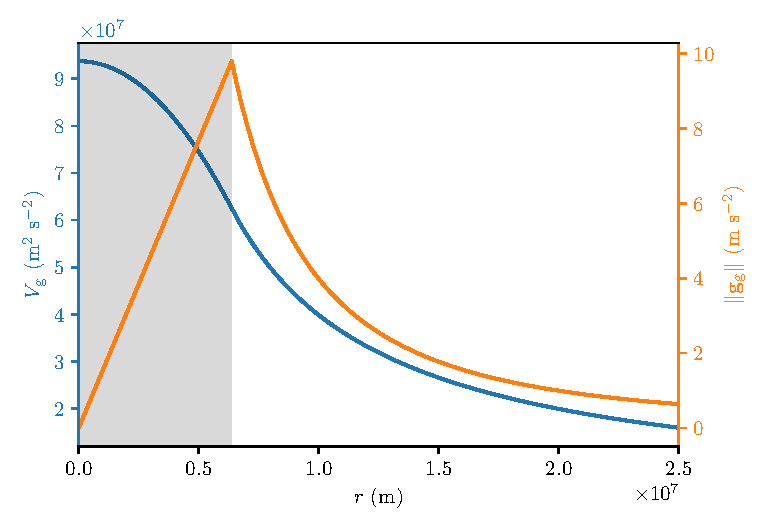
\includegraphics{./fig-homogeneous-ball-vg-gg.pdf}
\caption{Závislosť gravitačného potenciálu~$V_\gidx$ a~veľkosti gravitačného 
zrýchlenia~$\| \vec g_\gidx \|$ homogénnej gule od vzdialenosti~$r$ od ťažiska 
gule.  Hmotnosť gule je rovná hmotnosti Zeme, $M = 5.9722 \times 10^{24} 
\ \mathrm{kg}$, a~polomer gule je odvodený z~rovníkového polomeru Zeme, $R 
= 6\,378\,137\ \mathrm{m}$.  Tmavosivá plocha označuje oblasť vo vnútri gule.  
Obe veličiny majú samostatnú vertikálnu os.  Obrázok bol pripravený Zdrojovým 
kódom~\ref{src:ball} z~Prílohy~\ref{app:ball}.}
\label{fig:homogeneous_ball_plot}
\end{figure}

Obrázok~\ref{fig:homogeneous_ball_plot} možno vnímať ako najjednoduchšiu 
aproximáciu gravitačného potenciálu a~veľkosti gravitačného zrýchlenia v~okolí 
Zeme.  Presnejšou aproximáciou je model radiálne symetrickej Zeme, v~ktorom je 
hustota funkciou vzdialenosti od ťažiska Zeme.  Takýmto modelom je napríklad 
model PREM (angl. \emph{Preliminary Reference Earth Model}; 
\cite{Dziewonski1981}).  Ten ukazuje, že najväčšia veľkosť gravitačného 
zrýchlenia nie je na povrchu Zeme, ale v~hĺbke približne~$3000\ \mathrm{km}$ 
pod povrchom Zeme na rozhraní vonkajšieho jadra a~plášťa \parencite[pozri 
napríklad][]{TorgeGeodesy,Lowrie2007}.

\subsection{Tiažové pole homogénnej rotujúcej gule}
\label{sec:homogeneous_ball_gravity_field}

V~tejto časti stručne popíšeme tiažový potenciál a~tiažové zrýchlenie na 
povrchu homogénnej rotujúcej gule.  Budeme predpokladať, že homogénna guľa 
s~polomerom~$R$ rotuje okolo osi~$z$ konštantnou uhlovou rýchlosťou 
rotácie~$\omega$.  Na rozdiel od 
Kapitoly~\ref{sec:homogeneous_ball_gravitational_field}, tentokrát budeme 
uvažovať, že výpočtový bod sa môže nachádzať kdekoľvek \emph{na povrchu} gule.

Tiažový potenciál na povrchu homogénnej gule získame vzťahmi~(\ref{eq:vc}), 
(\ref{eq:w}) a~(\ref{eq:vg_ball_on}),
%
\begin{equation}
\label{eq:w_ball_on}
W(P) = \frac{GM}{R} + \frac{1}{2} \, \omega^2 \, R^2 \, \cos^2\varphi{.}
\end{equation}
%
Predošlý vzťah je funkciou sférickej šírky~$\varphi$, preto povrch homogénnej 
rotujúcej gule nie je ekvipotenciálna plocha.  Najväčší tiažový potenciál je na 
rovníku a~najmenší na póloch.

Tiažové zrýchlenie na povrchu gule získame \emph{vektorovým} súčtom 
(\ref{eq:g}) (Obrázok~\ref{fig:gravity_vector}).  Upozornime ale, že gravitačné 
zrýchlenie na povrchu gule zo vzťahu~(\ref{eq:gg_ball_on}) je vyjadrené 
v~súradnicovom systéme~$x^\mathrm{s}, y^\mathrm{s}, z^\mathrm{s}$, zatiaľ čo 
odstredivé zrýchlenie~(\ref{eq:gc}) je vyjadrené v~systéme~$x, y, z$.  Na 
výpočet tiažového zrýchlenia~$\vec g$ vektorovým súčtom~(\ref{eq:g}) je preto 
potrebné najprv vyjadriť oba vektory v~rovnakom súradnicovom systéme.  Ak 
postačuje vypočítať veľkosť tiažového zrýchlenia~$\| \vec g \|$, potom môžu byť 
použité vzťahy~(\ref{eq:gc_magnitude}) a~(\ref{eq:gg_ball_on_magnitude}).  Je 
potrebné však vziať do úvahy skutočnosť, že vektory~$\vec g_\gidx$ a~$\vec 
g_\cidx$ majú rozdielny smer a~tiež že tento smer závisí od sférickej 
šírky~$\varphi$ výpočtového bodu.  Veľkosť tiažového zrýchlenia je najväčšia na 
póloch, pretože na póloch je odstredivé zrýchlenie nulové.  Naopak, najmenšiu 
hodnotu dosahuje na rovníku, pretože odstredivé zrýchlenie je na rovníku 
najväčšie a~súčasne má opačný smer ako gravitačné zrýchlenie (pozri 
Obrázok~\ref{fig:gravity_vector}).

\section{Výšky}
\label{sec:heights}

Výšky prepájajú geometrický aspekt geodetického určovania polohy s~tiažovým 
poľom a~naopak.  Ak by sme o~výškach uvažovali iba z~pohľadu geometrie alebo 
iba z~pohľadu tiažového poľa, v~oboch prípadoch by sme získali výšky s~výrazne 
obmedzeným praktickým využitím.

V~Kapitole~\ref{sec:potential_differences} najprv vysvetlíme princíp určovania 
rozdielu tiažového potenciálu, ktorý priamo súvisí s~teóriou výšok, a~následne 
v~Kapitolách~\ref{sec:orthometric_height} až~\ref{sec:ellipsoidal_height} 
popíšeme vybrané typy výšok.  Pre rozsiahlosť problematiky však nepôjde 
o~vyčerpávajúce podanie, ale skôr o~poskytnutie základných informácií, ktoré sú 
potrebné pre pochopenie širšieho kontextu práce.  Podrobnosti a~ďalšie typy 
výšok je možné nájsť napríklad v~prácach \textcite{Jekeli2000a}, 
\textcite{MoritzPhysicalGeodesy} a~\textcite{SansoGeodeticHeights}.

\subsection{Určovanie rozdielu tiažového potenciálu}
\label{sec:potential_differences}

Hoci tiažový potenciál priamo odmerať nedokážeme 
(Kapitola~\ref{sec:centrifugal_and_gravity_potential}), \emph{rozdiel} 
tiažového potenciálu dokážeme určiť nepriamo kombináciou nivelácie 
a~gravimetrie.  Popis tejto metódy začneme vysvetlením pojmu totálny 
diferenciál.

\subsubsection{Totálny diferenciál}
\label{sec:total_diferential}

Ak sa poloha bodu~$P$ zmení o~vektor~$\delta \vec x$,
%
\begin{equation}
\label{eq:deltax}
\delta \vec x =
\begin{bmatrix}
\delta x\\
\delta y\\
\delta z
\end{bmatrix}
{,}
\end{equation}
%
potom tiažový potenciál~$W(P)$ sa zmení o~hodnotu~$\delta W(P, \delta \vec x)$.  
\emph{Totálny diferenciál}~$\diff W(P, \diff \vec x)$ aproximuje skutočnú zmenu 
tiažového potenciálu~$\delta W(P, \delta \vec x)$ vzťahom
%
\begin{equation}
\label{eq:w_totdiff_scalar}
\begin{split}
\delta W(P, \delta \vec x) \approx \diff W(P, \diff \vec x) &= 
\left.\frac{\partial W}{\partial x}\right|_P \, \diff x + \, 
\left.\frac{\partial W}{\partial y}\right|_P \, \diff y + \left.\frac{\partial 
W}{\partial z}\right|_P \, \diff z\\
%
&= \nabla W(P) \cdot \diff \vec x = \vec g(P) \cdot \diff \vec x = \| \vec g(P) 
\| \, \| \diff \vec x \| \, \cos\alpha{,}
\end{split}
\end{equation}
%
kde
%
\begin{equation}
\label{eq:diffx}
\diff \vec x =
\begin{bmatrix}
\diff x\\
\diff y\\
\diff z
\end{bmatrix}
\end{equation}
%
a~$\alpha$ je uhol medzi vektormi~$\vec g(P)$ a~$\diff \vec x$.  Skracovaním 
vzdialenosti~$\diff \vec x$ je možné zmenšiť aproximačnú chybu 
v~rovnici~(\ref{eq:w_totdiff_scalar}) na ľubovoľne malú hodnotu.  Vo 
všeobecnosti môžeme povedať, že totálny diferenciál (diferencovateľnej) 
funkcie~$f$ v~bode~$P$ je najlepšia lineárna aproximácia funkcie~$f$ v~okolí 
bodu~$P$.

Ak k~diferenciálnej zmene polohy~$\diff \vec x$ dochádza pozdĺž 
ekvipotenciálnej plochy, potom totálny diferenciál~$\diff W$ je nulový (pozri 
vektory~$\diff \vec x_2$ a~$\diff \vec x_4$ na 
Obrázku~\ref{fig:total_differential}).  Toto tvrdenie môžeme vysvetliť tým, že 
vektor~$\vec g$ je kolmý na ekvipotenciálnu plochu (a~tým aj na vektor~$\diff 
\vec x$), preto $\diff W = \| \vec g \| \, \| \diff \vec x \| \, 
\cos(90^{\circ}) = 0$.  Naopak, k~najväčšej zmene tiažového potenciálu dochádza 
vtedy, keď vektory~$\vec g$ a~$\diff \vec x$ majú rovnaký smer, to znamená keď 
vektor~$\diff \vec x$ je kolmý na ekvipotenciálnu plochu (pozri vektor~$\diff 
\vec x_1$ na Obrázku~\ref{fig:total_differential}).  V~takom prípade~$\alpha 
= 0$, preto $\diff W = \| \vec g \| \, \| \diff \vec x \| \, \cos(0) = \| \vec 
g \| \, \| \diff \vec x \|$.

\begin{figure}
\centering
\input{./fig-total-differential.pdf_tex}
\caption{Totálny diferenciál~$\diff W(P, \diff \vec x)$ v~bode~$P$.  Skúmaná je 
zmena tiažového potenciálu~$W(P)$ po zmene súradníc bodu~$P$ o~hodnoty~$\diff 
\vec x_1$ až~$\diff \vec x_5$.  Vektory~$\diff \vec x_1$ a~$\diff \vec x_3$ sú 
kolmé na ekvipotenciálnu plochu~$W(P) = \textrm{kon\v{s}t.}$, vektory~$\diff 
\vec x_2$ a~$\diff \vec x_4$ ležia v~jej dotykovej rovine a~symbol~$\diff \vec 
x_5$ označuje vektor vo všeobecnom smere.}
\label{fig:total_differential}
\end{figure}

\subsubsection{Geopotenciálna kóta}
\label{sec:geopotential_number}

Vráťme sa teraz k~určovaniu rozdielu tiažového potenciálu.  Ak dochádza 
k~diferenciálnej zmene polohy~$\diff \vec x$ pozdĺž tiažnice v~smere vektora 
$-\vec g$ (pozri vektor~$\diff \vec x_3$ na 
Obrázku~\ref{fig:total_differential}), potom medzi vektormi~$\vec g$ a~$\diff 
\vec x$ je uhol~$180^{\circ}$ a~totálny diferenciál tiažového potenciálu je 
daný vzťahom
%
\begin{equation}
\label{eq:w_totdiff_plumb}
\diff W(P, \diff \vec x) = \vec g(P) \cdot \diff \vec x = g(P) \, \diff H \, 
\cos(180^{\circ}) = -g(P) \, \diff H{,}
\end{equation}
%
kde~$g(P) = \| \vec g(P) \|$ je veľkosť tiažového zrýchlenia v~bode~$P$ 
a~$\diff H = \| \diff \vec x \|$ je diferenciálna dĺžka tiažnice.  Integráciou 
rovnice~(\ref{eq:w_totdiff_plumb}) od bodu~$A$ po bod~$B$ (pozri 
Obrázok~\ref{fig:total_differential}) získame rozdiel tiažového potenciálu,
%
\begin{equation}
\label{eq:w_ab}
W(B) - W(A) = \int\limits_{W(A)}^{W(B)} \diff W = -\int\limits_{P = A}^{B} g(P) 
\, \diff H = -\int\limits_{A}^{B} g \, \diff H{,}
\end{equation}
%
kde symboly~$W(A)$ a~$W(B)$ označujú tiažový potenciál v~bodoch~$A$ a~$B$.  
Osobitný význam pre fyzikálnu geodéziu má rozdiel tiažového potenciálu~$W_0$ na 
geoide v~bode~$P_0$ a~tiažového potenciálu~$W = W(P)$ v~bode~$P$ 
(Obrázok~\ref{fig:total_differential}).  Táto veličina sa nazýva 
\emph{geopotenciálna kóta} a~je daná vzťahom
%
\begin{equation}
\label{eq:geopotential_number}
C = W_0 - W = \int\limits_0^H g \, \diff H{,}
\end{equation}
%
kde~$H$ je dĺžka tiažnice od bodu~$P_0$ po bod~$P$.

Geopotenciálnu kótu je možné určiť pomocou nivelácie~($\diff H$) 
a gravimetrie~($g$).  Namiesto jednotky~$\mathrm{m}^2\ \mathrm{s}^{-2}$ sa 
niekedy zvykne udávať v~geopotenciálnych jednotkách~gpu,
%
\begin{equation}
\label{eq:gpu_unit}
1\ \mathrm{gpu} = 1\ \mathrm{kGal} \ \mathrm{m} = 1000\ \mathrm{Gal}\ 
\mathrm{m} = 10\ \mathrm{m}^2 \ \mathrm{s}^{-2}{.}
\end{equation}
%
V~súčasnosti je možné určiť rozdiel tiažového potenciálu s~presnosťou približne 
$\pm 0.1\ \mathrm{Gal} \ \mathrm{m}$ na vzdialenosť jedného kilometra 
\parencite{MoritzPhysicalGeodesy}.

\subsection{Ortometrická výška}
\label{sec:orthometric_height}

Rovnice~(\ref{eq:w_totdiff_plumb}) a~(\ref{eq:w_ab}) a~ich rôzne obmeny sa 
spolu so~vzťahom~(\ref{eq:geopotential_number}) využívajú na definíciu 
rozličných typov výšok 
\parencite{Jekeli2000a,MoritzPhysicalGeodesy,SansoGeodeticHeights}.  Ak totiž 
z~rovnice~(\ref{eq:w_totdiff_plumb}) vyjadríme diferenciál~$\diff H$ a~získanú 
rovnicu zintegrujeme od~$W_0$ po~$W$, dostaneme vzťah na výpočet dĺžky tiažnice 
od bodu~$P_0$ na geoide po bod~$P$ (Obrázok~\ref{fig:total_differential}),
%
\begin{equation}
\label{eq:orthometric_height_1}
H = -\int\limits_{W_0}^{W} \frac{\diff W}{g} = \int\limits_{0}^{C} \frac{\diff 
C}{g}{.}
\end{equation}
%
Pre praktické aplikácie je výhodné upraviť túto rovnicu nasledovne.  Prepíšme 
najprv rovnicu~(\ref{eq:geopotential_number}) do tvaru 
\parencite{MoritzPhysicalGeodesy}
%
\begin{equation}
\label{eq:geopotential_number_2}
C = H \, \frac{1}{H} \, \int\limits_0^H g \, \diff H = H \, \bar{g}{,}
\end{equation}
%
kde
%
\begin{equation}
\label{eq:mean_g_plumbline}
\bar{g} = \frac{1}{H} \, \int\limits_0^H g \, \diff H
\end{equation}
%
je priemerná hodnota tiažového zrýchlenia pozdĺž tiažnice medzi bodmi~$P_0$ 
a~$P$.  Z~rovnice~(\ref{eq:geopotential_number_2}) potom získame vzťah
%
\begin{equation}
\label{eq:orthometric_height_2}
H = H^\mathrm{O} = \frac{C}{\bar{g}}{,}
\end{equation}
%
Výška~$H^\mathrm{O}$ definovaná rovnicou~(\ref{eq:orthometric_height_2}) sa 
nazýva \emph{ortometrická výška} a~udáva dĺžku tiažnice od geoidu po bod~$P$ 
(Obrázky~\ref{fig:equipotential_surfaces} a~\ref{fig:total_differential}).

Z~Kapitoly~\ref{sec:potential_differences} vieme, že geopotenciálnu kótu~$C$ je 
možné odmerať nepriamo pomocou nivelácie a~gravimetrie.  Na výpočet 
ortometrickej výšky vzťahom~(\ref{eq:orthometric_height_2}) by preto malo 
postačovať určiť už iba priemernú hodnotu tiažového zrýchlenia~$\bar{g}$ pozdĺž 
tiažnice od geoidu po bod, ktorého výšku chceme získať.  Exaktný výpočet 
člena~$\bar{g}$ vzťahom~(\ref{eq:mean_g_plumbline}) je však nemožný.  Dôvod je 
ten, že integrál~(\ref{eq:mean_g_plumbline}) musí byť počítaný v~hmotách, ktoré 
sa nachádzajú medzi geoidom a~daným bodom.  Na takýto výpočet je potrebné 
poznať hustotu pozdĺž integračnej cesty (pozri hustotu~$\rho$ vystupujúcu vo 
vzťahu na výpočet gravitačného zrýchlenia v~rovnici~\ref{eq:gg_body}).  
Hustotné modely, ktoré by mohli byť použité na tento účel, sú v~istej miere 
dostupné \parencite[napríklad][]{Sheng2019}, no ich presnosť sa zdá byť ešte 
stále nepostačujúca.  Praktická realizácia ortometrických výšok teda závisí od 
prijatého hustotného modelu.

Ďalšou nevýhodou ortometrických výšok je skutočnosť, že body na jednej 
ekvipotenciálnej ploche (za ideálnych podmienok napríklad na ustálenej vodnej 
hladine jazera) majú vo všeobecnosti \emph{rôznu} ortometrickú výšku.  
Ortometrické výšky teda nedostatočne reflektujú smer tečenia vody.  Tento 
problém majú všetky výšky okrem dynamických výšok 
(Kapitola~\ref{sec:dynamic_height}).

\subsubsection{Helmertova ortometrická výška}
\label{sec:helmert_height}

\emph{Helmertova ortometrická výška} je jedna z~približných realizácií 
ortometrickej výšky.  Definovaná je vzťahom
%
\begin{equation}
\label{eq:helmert_height}
H^\mathrm{HO} = \frac{C}{g + 0.0424\ \mathrm{mGal} \, \mathrm{m}^{-1} 
\ H^\mathrm{HO}}{.}
\end{equation}
%
Vzťah~$g + 0.0424\ \mathrm{mGal} \, \mathrm{m}^{-1}$ sa nazýva 
\emph{Poincarého--Preyova} redukcia tiažového zrýchlenia a~približne modeluje 
skutočné tiažové zrýchlenie \emph{v~hmotách}.  Symbol~$g$ označuje tiažové 
zrýchlenie na povrchu Zeme.  Konštanta~$0.0424\ \mathrm{mGal} \, 
\mathrm{m}^{-1}$ bola vypočítaná pre strednú hustotu hmôt nad geoidom 
s~použitím hustoty~$2670\ \mathrm{kg} \ \mathrm{m}^{-3}$ \parencite[pre 
odvodenie pozri 
napríklad][]{Jekeli2000a,MoritzPhysicalGeodesy,SansoGeodeticHeights}.  
F.~R.~Helmert~(1843~-- 1917) bol nemecký geodet a~štatistik.  Je autorom 
napríklad 7-prvkovej podobnostnej transformácie medzi trojrozmernými 
karteziánskymi súradnicovými systémami.

\subsection{Dynamická výška}
\label{sec:dynamic_height}

\emph{Dynamická výška} je definovaná ako podiel geopotenciálnej kóty bodu, 
ktorého výšku určujeme, a~\emph{zvolenej konštantnej} hodnoty tiažového 
zrýchlenia,
%
\begin{equation}
\label{eq:dynamic_height}
H^\mathrm{D} = \frac{C}{g_\textrm{kon\v{s}t.}}{.}
\end{equation}

Po uvážení vzťahov~$C = W_0 - W$ (rovnica~\ref{eq:geopotential_number}) 
a~(\ref{eq:dynamic_height}) je zrejmé, že body na tej istej ekvipotenciálnej 
ploche majú \emph{konštantnú} dynamickú výšku.  Mohlo by sa teda zdať, že 
dynamická výška rieši problém, ktorým sú zaťažené všetky ostatné typy výšok 
(pozri Kapitolu~\ref{sec:orthometric_height}).  V~skutočnosti je však azda 
najmenej praktická.  Kvôli konštantnej hodnote~$g_{\textrm{konšt.}}$ je 
dynamická výška iba akýmsi preškálovaním geopotenciálnej kóty z~fyzikálnych 
jednotiek~$\mathrm{m}^2 \ \mathrm{s}^{-2}$ do jednotky dĺžky~$\mathrm{m}$.  
Neberie tak do úvahy skutočnosť, že body na dvoch rozdielnych ekvipotenciálnych 
plochách môžu byť od seba rozlične geometricky vzdialené (porovnaj vzdialenosti 
medzi ekvipotenciálnymi plochami v~oblasti rovníka a~v~oblastiach pólov na 
Obrázku~\ref{fig:equipotential_surfaces}).  Dynamická výška je teda výhradne 
fyzikálna veličina, ktorá nemá geometrickú interpretáciu 
\parencite{Jekeli2000a}.

Vidíme, že koncept výšky bez uváženia geometrie je nepraktický.  Takéto výšky 
sú použiteľné nanajvýš na regionálnej úrovni, kde tieto nedostatky dosahujú 
zanedbateľné vplyvy voči presnosti geodetických meraní.  V~nasledujúcej 
kapitole sa presvedčíme, že to isté platí aj o~výškach, ktoré neberú do úvahy 
tiažové pole.

\subsection{Elipsoidická výška}
\label{sec:ellipsoidal_height}

Nech je daný referenčný elipsoid s~hlavnou polosou~$a$ a~vedľajšou polosou~$b$.  
Polohu bodu~$P$ voči tomuto referenčnému elipsoidu môžeme vyjadriť pomocou 
elipsoidických súradníc.  Tieto súradnice budeme označovať symbolmi $\phi, 
\lambda, h$, pričom~$\phi$ je elipsoidická šírka, $\lambda$~je elipsoidická 
dĺžka~a~$h$ je elipsoidická výška (Obrázok~\ref{fig:ell_coords}).  
\emph{Elipsoidická výška} je vzdialenosť bodu~$P$ od referenčného elipsoidu 
meraná po normále k~tomuto elipsoidu.

\begin{figure}[bt]
\centering
\input{./fig-ell-coords.pdf_tex}
\caption{Elipsoidická šírka~$\phi$ a~elipsoidická výška~$h$ bodu~$P$.  
Elipsoidická dĺžka~$\lambda$ je totožná so sférickou dĺžkou (pozri 
Obrázok~\ref{fig:cart_sph}), pretože referenčný elipsoid je dvojosový.}
\label{fig:ell_coords}
\end{figure}

Elipsoidickú výšku je možné jednoducho vypočítať z~meraní, ktoré využívajú 
globálne navigačné družicové systémy (GNSS).  Zatiaľ čo dynamická výška má 
výhradne fyzikálny význam, elipsoidická výška má výhradne geometrický význam.  
Pre aplikácie, ktoré vyžadujú uvážiť aspoň do určitej miery smer tečenia vody 
(resp. vplyv tiažového poľa), je elipsoidická výška nevhodná.  Lepším riešením 
je použiť napríklad ortometrickú výšku (Kapitola~\ref{sec:orthometric_height}).  
Rozdiel medzi elipsoidickou výškou a~ortometrickou výškou môže dosahovať až 
desiatky metrov a~výrazne varíruje s~polohou, dokonca i~na regionálnej úrovni.  
V~praktických aplikáciách sa elipsoidická výška vypočítaná z~GNSS meraní často 
zvykne transformovať na inú výšku, napríklad na ortometrickú výšku.  Vzťah 
medzi ortometrickou a~elipsoidickou výškou bude diskutovaný neskôr 
v~Kapitole~\ref{sec:geoid}.

Na záver doplňme transformáciu elipsoidických súradníc na karteziánske 
súradnice \parencite{MoritzPhysicalGeodesy}
%
\begin{equation}
\begin{split}
x &= (N + h) \, \cos\phi \, \cos\lambda{,}\\
y &= (N + h) \, \cos\phi \, \sin\lambda{,}\\
z &= \left[ N \, (1 - e^2) + h \right] \, \sin\phi{,}\\
\end{split}
\end{equation}
%
kde
%
\begin{equation}
\label{eq:curvature_N}
N = \frac{a}{\sqrt{1 - e^2 \, \sin^2\phi}}
\end{equation}
%
je \emph{priečny polomer krivosti} a
%
\begin{equation}
\label{eq:1st_eccentricity}
e = \frac{\sqrt{a^2 - b^2}}{a}
\end{equation}
%
je \emph{prvá numerická excentricita}.  Presná a~efektívna inverzná 
transformácia je predmetom geodetického záujmu niekoľko dekád.  Prehľad metód 
a~príslušné vzťahy je možné nájsť napríklad 
v~publikáciách~\textcite{Fukushima2006} a~\textcite{Claessens2019}.



\section{Časové variácie}
\label{sec:time_variable_gravity}

Z~Newtonovho integrálu~(\ref{eq:vg_body}) vyplýva, že gravitačné pole závisí od 
tvaru telesa, rozloženia hustoty v~jeho vnútri a~od polohy bodu vzhľadom 
k~telesu.  Zmenou tvaru telesa, a~tým aj polohy výpočtového bodu voči telesu, 
alebo zmenou hustoty telesa v~čase dochádza k~zmene gravitačného poľa v~čase.  
Ak navyše teleso rotuje a~polohu vyjadrujeme v~neinerciálnom súradnicovom 
systéme, ktorý rotuje spolu s~telesom, potom vzniká aj odstredivé pole.  Časová 
zmena odstredivého poľa, spôsobená napríklad premenlivou uhlovou rýchlosťou 
rotácie, potom spôsobuje časovú zmenu tiažového poľa.  V~tejto kapitole 
spomenieme niektoré príčiny, ktoré spôsobujú časovú variáciu gravitačného 
a~tiažového poľa v~okolí Zeme.

V~tiažovom zrýchlení odmeranom gravimetrickými metódami (pozri 
Kapitolu~\ref{sec:gravity_measurements} a~najmä~\cite{Janak2010}) je obsiahnutý 
gravitačný účinok všetkých hmotných objektov vo vesmíre.  Okrem samotnej Zeme 
majú merateľný gravitačný vplyv predovšetkým Mesiac a~Slnko a~v~oveľa menšej 
miere aj Venuša, Jupiter a~Mars.  Gravitačný vplyv týchto objektov budeme 
nazývať \emph{slapové zrýchlenie} alebo tiež \emph{priame slapy}.  Na výpočet 
slapového zrýchlenia je potrebné poznať polohu bodu merania a~polohu nebeských 
telies v~okamihu merania.  Podľa \textcite{Torge1989} dosahuje slapové 
zrýchlenie spôsobené Mesiacom a~Slnkom na povrchu Zeme maximálne hodnoty 
približne~$0.165\ \mathrm{mGal}$ a~$0.075\ \mathrm{mGal}$.  Vzhľadom na súčasnú 
mikroGalovú presnosť gravimetrických meraní tak ide nezanedbateľný vplyv.

V~predošlom odseku sme uvažovali, že Zem je dokonale tuhé teleso, ktoré nie je 
deformované slapovými silami.  V~presnejšom priblížení je Zem pružné teleso, 
ktoré vplyvom slapových síl mení svoj tvar.  V~dôsledku zmeny tvaru pevnej 
a~oceánskej časti zemského povrchu tak vznikajú \emph{zemské} a~\emph{oceánske 
slapy}.  Tento jav sa tiež nazýva \emph{nepriame slapy}.  Oceánske slapy 
vysvetlil I.~Newton \parencite{Torge1989}.  Na zemské slapy poukázal William 
Thomson, známy skôr pod šľachtickým menom Lord Kelvin~(1824~-- 1907) (tamtiež).  
V~dôsledku zemských slapov je potrebné navýšiť súčet slapových efektov 
z~predošlého odseku približne~o~16~\%, čím získame maximálny súhrnný 
efekt~$0.280\ \mathrm{mGal}$ \parencite{Torge1989}.  V~závislosti od lokality 
dosahujú oceánske slapy hodnoty približne~$0.010\ \mathrm{mGal}$ až~$0.001\ 
\mathrm{mGal}$ \parencite{Torge1989}.

Rotačná os Zeme neustále mení svoju polohu voči Zemi.  Jedným z~dôsledkov je 
\emph{pohyb pólu}, ktorý na povrchu Zeme dosahuje niekoľko metrov (desatín 
uhlovej sekundy) za rok \parencite{MoritzPhysicalGeodesy}.  Pohyb rotačnej osi 
tak spôsobuje zmenu súradníc bodov na povrchu Zeme ako aj~zmenu odstredivého 
(rovnica~\ref{eq:gc}) a~tiažového zrýchlenia (rovnica~\ref{eq:g}).  Pohyb pólu 
má najväčší vplyv na tiažové zrýchlenie v~oblastiach so zemepisnou 
šírkou~$45^{\circ}$, kde nadobúda maximálnu hodnotu približne~$0.008\ 
\mathrm{mGal}$ \parencite{Torge1989}.  Okrem polohy rotačnej osi sa mení aj 
uhlová rýchlosť rotácie Zeme.  Jej vplyv na zmenu tiažového zrýchlenia však nie 
je väčší ako zhruba~$0.0007\ \mathrm{mGal}$ \parencite{Torge1989}.

Zmeny gravitačného a~tiažového poľa v~okolí Zeme môžu byť spôsobené aj mnohými 
ďalšími faktormi, vymenujme aspoň pohyb magmy v~zemskom plášti, postglaciálny 
zdvih, seizmické vlny, hydrologické zmeny, roztápanie ľadovcov a pod.  
V~literatúre sa niekedy diskutuje aj o~časovej variácii Newtonovej gravitačnej 
konštanty~$G$.  Tento jav však doposiaľ nebol experimentálne potvrdený 
\parencite{Torge1989}.






% -----------------------------------------------------------------------------

\chapter{Sférický harmonický rozvoj}
\label{sec:spherical_harmonic_expansion}

Newtonov integrál~(\ref{eq:vg_body}) nie je vhodný na priamy praktický výpočet 
gravitačného poľa Zeme.  Predpokladá totiž, že poznáme dve matematické funkcie: 
jednu, ktorá definuje tvar Zeme a~druhú, ktorá opisuje jej hustotu.  
Problematická je obzvlášť hustota.  Hoci približné hustotné modely zemského 
telesa existujú \parencite[napríklad][]{Dziewonski1981}, pre ich nízku presnosť 
nedokážeme vzťahom~(\ref{eq:vg_body}) naplniť súčasné nároky na modelovanie 
gravitačného poľa Zeme.  Postačujúce nie sú ani regionálne hustotné modely, 
a~to napriek tomu, že sú presnejšie ako globálne modely.  V~tejto kapitole 
popíšeme jeden z~praktických spôsobov modelovania gravitačného poľa Zeme 
\emph{bez potreby priamej znalosti hustoty}.






\section{Motivácia}
\label{sec:sh_motivation}

Nech je daný trojrozmerný karteziánsky súradnicový systém so začiatkom 
v~bode~$O$ a~so súradnicovými osami~$x, y, z$ (Obrázok~\ref{fig:unit_vectors}).  
Symbolmi~$\vec e_1, \vec e_2, \vec e_3$ označme jednotkové vektory v~smere 
súradnicových osí (rovnica~\ref{eq:unit_vectors}).  Nech~$\vec r$ je ľubovoľný 
vektor v~tomto priestore,
%
\begin{figure}
\centering
\input{./fig-vector-in-3d.pdf_tex}
\caption{Polohový vektor~$\vec r$ bodu~$P$ v~trojrozmernom karteziánskom 
súradnicovom systéme.}
\label{fig:unit_vectors}
\end{figure}

\begin{equation}
\vec r =
\begin{bmatrix}
r_1\\
r_2\\
r_3
\end{bmatrix}
{.}
\end{equation}

Jednotkové vektory majú tú vlastnosť, že umožňujú vyjadriť ľubovoľný vektor
$\vec r$ vzťahom
%
\begin{equation}
\label{eq:r_synthesis}
\vec r = \sum_{i = 1}^3 r_i \, \vec e_i{.}
\end{equation}
%
Koeficient~$r_i$ predstavuje váhu, ktorou sa jednotkový vektor~$\vec e_i$ 
podieľa na lineárnej kombinácii~(\ref{eq:r_synthesis}).  Môžeme tiež povedať, 
že koeficienty~$r_i$ sú súradnice koncového bodu vektora~$\vec r$.  Takýmto 
bodom môže byť napríklad bod na povrchu Zeme v~geocentrickom karteziánskom 
súradnicovom systéme.  Nie je náročné presvedčiť sa, že koeficient~$r_i$ je 
daný skalárnym súčinom vektora~$\vec r$ a~príslušného jednotkového 
vektora~$\vec e_i$,
%
\begin{equation}
\label{eq:r_analysis}
r_i = \vec r \cdot \vec e_i{.}
\end{equation}

Povedané slovne, vzťah~(\ref{eq:r_synthesis}) hovorí, že ak poznáme koeficienty 
$r_i$, poznáme vektor~$\vec r$.  Vzťah~(\ref{eq:r_analysis}) hovorí, ako tieto 
koeficienty vypočítať z~vektora~$\vec r$.  Bolo by výhodné, ak by sme obdobným 
spôsobom dokázali vyjadriť aj gravitačný potenciál~$V_\gidx$, teda istým 
spôsobom ho rozložiť na súradnice a~následne ho z~týchto súradníc 
zrekonštruovať.  Samozrejme, gravitačný potenciál nepatrí do vyššie opísaného 
trojrozmerného priestoru vektorov~$\vec r$.  V~abstraktnejšom chápaní slova 
priestor je však aj gravitačný potenciál súčasťou nejakého priestoru, napríklad 
priestoru funkcií, ktoré sú harmonické mimo Zeme.  Vieme už, že medzi takéto 
funkcie patrí okrem gravitačného potenciálu napríklad aj funkcia~$1 \slash 
\ell$, pričom~$\ell$ je v~tomto prípade vzdialenosť bodu nachádzajúceho sa mimo 
Zeme od diferenciálneho hmotného elementu Zeme (pozri 
Obrázok~\ref{fig:gravitating_body} a~rovnice~\ref{eq:nabla_l} 
a~\ref{eq:l_2nd_derivatives}).  Takýchto funkcií je nespočetné množstvo 
a~v~matematickom zmysle tvoria istý priestor.  Podobne ako v~trojrozmernom 
priestore vektorov~$\vec r$, i~v tomto priestore možno nájsť matematické 
objekty, ktorými môžeme každý prvok patriaci do tohto priestoru, napríklad 
gravitačný potenciál, rozložiť na súradnice,
%
\begin{equation}
\label{eq:vg_analysis}
v_{nk} = \frac{N^2_{nk}}{4\pi} \, \iint\limits_{\sigma} V_\gidx(r, \varphi, 
\lambda) \, Y_{nk}(\varphi, \lambda) \, \diff \sigma{,}
\end{equation}
%
a~následne ho spätne zrekonštruovať,
%
\begin{equation}
\label{eq:vg_synthesis}
V_\gidx(r, \varphi, \lambda) = \sum_{n = 0}^{\infty} \sum_{k = -n}^{n} v_{nk}
\, Y_{nk}(\varphi, \lambda){.}
\end{equation}
%
Koeficienty~$v_{nk}$ vo vzťahu~(\ref{eq:vg_analysis}) predstavujú súradnice
gravitačného potenciálu~$V_\gidx(r, \varphi, \lambda)$ vo vyššie opísanom
abstraktom priestore harmonických funkcií mimo Zeme a~symbol~$Y_{nk}(\varphi, 
\lambda)$
označuje \emph{sférické harmonické funkcie}.  Koeficienty~$N_{nk}$ závisia
iba od~$n$ a~$k$ a~budú diskutované neskôr.  Vzťah~(\ref{eq:vg_analysis}) je
tak obdobou vzťahu (\ref{eq:r_analysis}), súradnice~$v_{nk}$ možno prirovnať
k~súradniciam~$r_i$ a~sférické harmonické funkcie~$Y_{nk}(\varphi, \lambda)$
možno prirovnať k~jednotkovým vektorom~$\vec e_i$.  Samotný integrál na
jednotkovej sfére~$\sigma$ možno chápať ako skalárny súčin funkcií~$V_\gidx$
a~$Y_{nk}$, ktorý je obdobou skalárneho súčinu vektorov~$\vec r \cdot \vec
e_i$.  Pokiaľ ide o~vzťah~(\ref{eq:vg_synthesis}), ten plní podobnú úlohu ako
rovnica~(\ref{eq:r_synthesis}), teda umožňuje zrekonštruovať gravitačný
potenciál z~jeho súradníc~$v_{nk}$.

Je zrejmé, že v~prípade gravitačného potenciálu (rovnice \ref{eq:vg_analysis}
a~\ref{eq:vg_synthesis}) je situácia komplikovanejšia ako v~prípade polohových
vektorov (rovnice \ref{eq:r_synthesis} a~\ref{eq:r_analysis}).  Súradníc
$v_{nk}$ je nekonečne veľa (pozri limity prvej sumácie vo
vzťahu~\ref{eq:vg_synthesis}), sumácia je dvojitá a~sférické harmonické funkcie
$Y_{nk}(\varphi, \lambda)$ závisia od sférickej šírky~$\varphi$ a~sférickej
dĺžky~$\lambda$.  Napriek tomu, samotný princíp zostáva rovnaký a~demonštruje, 
že ak poznáme súradnice~$v_{nk}$, potom
integrály~(\ref{eq:gg_body}) a~(\ref{eq:vg_body}) vieme vypočítať aj bez
priameho použitia hustoty.  Hustota Zeme je pritom obsiahnutá 
v~súradniciach~$v_{nk}$.  Cieľom nasledujúcich strán je ukázať, akým spôsobom 
sa v~nich táto hustota nachádza, ako je možné prejsť od 
vzťahu~(\ref{eq:vg_body}) až k~formálne veľmi odlišnému 
vzťahu~(\ref{eq:vg_synthesis}) a~tiež ukázať, ako je možné vypočítať 
súradnice~$v_{nk}$.



\section{Rozvoj gravitačného potenciálu do radu sférických harmonických
funkcií}
\label{sec:vg_sh_expansion}

V~tejto kapitole odvodíme vzťah~(\ref{eq:vg_synthesis})
z~rovnice~(\ref{eq:vg_body}).  Zavedených bude niekoľko nových pojmov, no aby 
sme pričasto neprerušovali prirodzený myšlienkový postup odvodenia, nové pojmy
predstavíme len vo forme nevyhnutnej na pochopenie samotného odvodenia.
Vrátime sa k~nim v~nasledujúcich kapitolách, podobne ako sa čitateľ môže neskôr 
vrátiť k~tejto kapitole.

Nech je dané všeobecné teleso s~objemom~$\tau$ a~hustotou~$\rho$
(Obrázok~\ref{fig:gravitating_body}).  Hustota~$\rho$ sa v~telese môže meniť,
no budeme predpokladať, že v~každom diferenciálnom elemente~$\diff \tau(Q)$ je
konečná.  Nech je ďalej daný bod~$P$, ktorý sa nachádza \emph{mimo} všeobecného
telesa, teda v~tej časti priestoru, v~ktorom je gravitačný potenciál harmonický
(Kapitola~\ref{sec:harmonic_function}).  Trojicu sférických súradníc 
(Obrázok~\ref{fig:cart_sph}) bodov~$P$ a~$Q$ označme symbolmi~$r, \varphi,
\lambda$~a~$r', \varphi', \lambda'$.  Symbolom~$\ell$ budeme označovať 
vzdialenosť medzi bodmi~$P$~a~$Q$ (rovnica~\ref{eq:l_sph} 
a~Obrázok~\ref{fig:distance_l}).

Upravme člen~$1 \slash \ell$ z~rovnice~(\ref{eq:vg_body}) pomocou 
vzťahu~(\ref{eq:l_sph}),
%
\begin{equation}
\label{eq:1l}
\begin{split}
\frac{1}{\ell} &= \frac{1}{\sqrt{ r^2 + (r')^2 - 2 \, r \, r' \, \cos\psi
}} = \frac{1}{r \, \sqrt{1 + \left( \dfrac{r'}{r}
\right)^2 - 2 \dfrac{r'}{r} \cos\psi}}\\
%
&=\frac{1}{r} \, \left[1 + \left( \dfrac{r'}{r}
\right)^2 - 2 \dfrac{r'}{r} \cos\psi \right]^{-\frac{1}{2}}{.}
\end{split}
\end{equation}
%
Ak by sme dosadili túto rovnicu do vzťahu~(\ref{eq:vg_body}), ďalšie 
matematické úpravy by sa vykonávali pomerne zložito, pretože hranatá zátvorka 
obsahuje tri sčítance umocnené na exponent~$-\frac{1}{2}$.  Výhodnejšie je 
rozvinúť tento člen do mocninového radu.  Jeden zo spôsobov rozvinutia funkcie 
do mocninového radu je pomocou Taylorovho, resp. Maclaurinovho radu.  
\emph{Maclaurinov rad} získame z~Taylorovho radu~(\ref{eq:f_taylor}), keď~$x_0 
= 0$,
%
\begin{equation}
\label{eq:f_maclaurin}
f(x) = \sum_{n = 0}^\infty \frac{1}{n!} \, \frac{\diff^n f(x)}{\diff x^n} 
\bigg\lvert_{x = 0} \, x^n{.}
\end{equation}
%
Zaveďme nasledovné substitúcie pre niektoré členy z~rovnice~(\ref{eq:1l}),
%
\begin{align}
\label{eq:alpha}
\alpha &= \frac{r'}{r}{,}\\
%
\label{eq:t}
t &= \cos\psi{,}\\
%
\label{eq:generic_function_for_lps}
H(\alpha, t) &= \left(1 + \alpha^2 - 2 \, \alpha\, t \right)^{-\frac{1}{2}}{.}
\end{align}
%
Ak
%
\begin{equation}
\label{eq:alpha_lt_1}
\alpha < 1{,}
\end{equation}
%
potom funkcia~$H(\alpha, t)$ môže byť rozvinutá do Maclaurinovho 
radu~(\ref{eq:f_maclaurin}),
%
\begin{equation}
\label{eq:maclaurin_series_of_generic_function}
H(\alpha, t) = \sum_{n = 0}^\infty \frac{1}{n!} \, \frac{\partial^n H(\alpha,
t)}{\partial \alpha^n} \bigg\lvert_{\alpha = 0} \, \alpha^n = \sum_{n 
= 0}^\infty P_n(t) \, \alpha^n{,}
\end{equation}
%
kde
%
\begin{equation}
\label{eq:pn}
P_n(t) = \frac{1}{n!} \, \frac{\partial^n H(\alpha, t)}{\partial \alpha^n} 
\bigg\lvert_{\alpha = 0}{.}
\end{equation}

Funkcie~$P_n(t)$ definované vzťahom~(\ref{eq:pn}) dostali názov podľa ich 
objaviteľa, francúzskeho matematika A.--M.~Legendrea, a~nazývajú sa 
\emph{Legendreove polynómy stupňa~$n$}.  Funkcia~$H(\alpha, t)$ sa nazýva 
\emph{generická funkcia pre Legendreove polynómy}.  Dosadením~(\ref{eq:pn}), 
(\ref{eq:maclaurin_series_of_generic_function}) 
a~(\ref{eq:generic_function_for_lps}) do~(\ref{eq:1l}) a~po uvážením 
substitúcií~(\ref{eq:alpha}) a~(\ref{eq:t}) získame rozvoj funkcie~$1 \slash 
\ell$ do radu Legendreových polynómov pre~$r > r'$ (pozri 
nerovnosť~\ref{eq:alpha_lt_1}),
%
\begin{equation}
\label{eq:1l_legpol}
\frac{1}{\ell} = \frac{1}{r} \, \sum_{n = 0}^\infty \left( \frac{r'}{r} 
\right)^{n} \, P_n(\cos\psi) = \frac{1}{r'} \, \sum_{n = 0}^\infty \left( 
\frac{r'}{r} \right)^{n + 1} \, P_n(\cos\psi){.}
\end{equation}
%
Dosadením prostredného výrazu z~poslednej rovnice do~(\ref{eq:vg_body}) 
dostaneme vzťah
%
\begin{equation}
\label{eq:vg_legpol}
V_\gidx(P) = \frac{G}{r} \, \iiint\limits_{\tau} \rho(r', \varphi', \lambda') 
\, \sum_{n = 0}^{\infty} \left( \frac{r'}{r} \right)^n \, P_n(\cos\psi) \, 
\diff\tau(Q){.}
\end{equation}

Z~pohľadu sférických súradníc je Legendreov polynóm~$P_n(\cos\psi)$ vo 
vzťahu~(\ref{eq:vg_legpol}) zložená funkcia, pretože je funkciou~$\cos\psi$, 
pričom samotná funkcia~$\cos\psi$ závisí od uhlovej časti sférických súradníc 
bodov~$P$ a~$Q$ (pozri rovnicu~\ref{eq:cospsi}).  Bolo by preto vhodné nájsť 
taký vzťah pre Legendreov polynóm~$P_n(\cos\psi)$,
v~ktorom by každá prípadná funkcia závisela iba od jednej z~premenných
$\varphi,  \lambda, \varphi', \lambda'$, a~nie od viacerých
premenných ako je tomu po dosadení~(\ref{eq:cospsi})
do~(\ref{eq:vg_legpol}).  Na tento účel slúži \emph{dekompozičný vzorec pre
Legendreove polynómy}, niekedy tiež nazývaný aj \emph{adičný teorém} či 
\emph{súčtová veta}.  Podľa \textcite{Hobson} bol adičný teorém po prvýkrát 
odvodený A.--M.~Legendreom v~roku~1782.  Odvodenie kvôli zložitosti vynecháme, 
no je možné nájsť ho napríklad v~sekcii~90 Kapitoly~IV knihy \textcite{Hobson}.

Dekompozičný vzorec pre Legendreove polynómy možno zapísať vo viacerých
ekvivalentných formách, napríklad
\parencite{Hobson,MoritzPhysicalGeodesy,SansoGeoidDetermination}
%
\begin{equation}
\label{eq:pn_decomposition_formula}
\begin{split}
P_n(\cos\psi) &= P_n(\sin\varphi) \, P_n(\sin\varphi')\\
%
&\phantom{={}} +2 \sum_{m = 1}^{n} \frac{(n - m)!}{(n + m)!} \,
P_{nm}(\sin\varphi) \, P_{nm}(\sin\varphi') \, \cos\left[m (\lambda
- \lambda') \right]\\
%
&= \sum_{m = 0}^{n} (2 - \delta_{m0}) \, \frac{(n - m)!}{(n + m)!} \, \left[
P_{nm}(\sin\varphi) \, \cos(m\lambda) \, P_{nm}(\sin\varphi') \,
\cos(m\lambda')\right.\\
%
&\phantom{={}}+\left. P_{nm}(\sin\varphi) \, \sin(m\lambda) \,
P_{nm}(\sin\varphi') \, \sin(m\lambda')\right]{.}
\end{split}
\end{equation}
%
Novozavedený člen~$P_{nm}(t)$, $t \in [-1, 1]$, sa nazýva \emph{pridružená 
Legendreova funkcia prvého druhu}
a~je daný vzťahom
%
\begin{equation}
\label{eq:pnm_def}
P_{nm}(t) = (1 - t^2)^{m \slash 2} \, \frac{\diff^m P_n(t)}{\diff t^m}{.}
\end{equation}
%
Symbol~$m$ sa nazýva \emph{rád} a~môže nadobúdať hodnoty $m = 0, 1, \dots, n$ 
(pozri druhú sumáciu vo vzťahu~\ref{eq:pn_decomposition_formula}).  Zo 
vzťahu~(\ref{eq:pnm_def}) vidíme, že Legendreova funkcia stupňa~$n$ a~rádu~$m$ 
súvisí s~$m$-tou deriváciou Legendreoveho polynómu stupňa $n$ podľa 
premennej~$t$.  Všimnime si, že Legendreova funkcia stupňa~$n$ a~rádu~$m = 0$ 
je totožná s~Legendreovým polynómom stupňa~$n$, $P_{n0}(t) = P_n(t)$.   Vo 
vzťahu~(\ref{eq:pn_decomposition_formula}) pribudol ešte člen~$\delta_{m0}$, 
ktorý má názov Kroneckerovo delta.  Všeobecná definícia pre~$m$ a~$\ell$ má 
tvar
%
\begin{equation}
\delta_{ml} =
%
\begin{cases}
1{,} \quad \mathrm{ak} \quad m = \ell{,}\\
0{,} \quad \mathrm{ak} \quad m \neq \ell{.}
\end{cases}
\end{equation}

Dosadením~(\ref{eq:pn_decomposition_formula}) do~(\ref{eq:vg_legpol})
získame výsledný vzťah
%
\begin{equation}
\label{eq:vg_sh_no_norm}
V_\gidx(P) = G \sum_{n = 0}^\infty \frac{1}{r^{n + 1}} \sum_{m = 0}^{n} \left(
C_{nm} \, \cos(m\lambda) + S_{nm} \, \sin(m\lambda)\right) \,
P_{nm}(\sin\varphi){,}
\end{equation}
%
kde
%
\begin{equation}
\label{eq:vg_shc_no_norm}
\begin{rcases}
C_{nm}\\
S_{nm}
\end{rcases}
= (2 - \delta_{m0}) \frac{(n - m)!}{(n + m)!} \iiint\limits_{\tau} \rho(r',
\varphi', \lambda') \, (r')^n \, P_{nm}(\sin\varphi')
%
\begin{Bmatrix}
\cos(m\lambda')\\
\sin(m\lambda')
\end{Bmatrix}
%
\diff\tau(Q){.}
\end{equation}
%
Všimnime si, že vo vzťahu~(\ref{eq:vg_sh_no_norm}) sú premennými iba súradnice 
$r, \varphi, \lambda$ výpočtového bodu~$P$, v~ktorom určujeme gravitačný 
potenciál (pozri Obrázok~\ref{fig:gravitating_body}).  Naproti tomu, vo 
vzťahu~(\ref{eq:vg_shc_no_norm}) sú premenné iba súradnice $r',\varphi', 
\lambda'$ diferenciálneho elementu~$\diff\tau(Q)$ 
(Obrázok~\ref{fig:gravitating_body}).  Ďalej vidíme, že koeficienty~$C_{nm}$ 
a~$S_{nm}$ sú pre dané teleso \emph{konštantné}.  Ak teda poznáme 
koeficienty~$C_{nm}$ a~$S_{nm}$, potom vďaka vzťahu~(\ref{eq:vg_sh_no_norm}) 
poznáme gravitačný potenciál~$V_\gidx$ v~(takmer) ľubovoľnom bode~$P$ mimo 
daného telesa.  Nepripomína to situáciu z~Kapitoly~\ref{sec:sh_motivation}, 
v~ktorej sme tvrdili, že ak poznáme súradnice~$r_i$ vektora~$\vec r$, potom 
poznáme vektor~$\vec r$?  Hoci to ešte nemusí byť na prvý pohľad zrejmé, 
koeficienty $C_{nm}$ a~$S_{nm}$ sú v~skutočnosti veľmi úzko spojené so 
súradnicami~$v_{nm}$ z~rovnice~(\ref{eq:vg_synthesis}).

Po nahradení nekonečna nezáporným celým číslom~$N$ je možné 
vzťah~(\ref{eq:vg_sh_no_norm}) i~prakticky vypočítať.  V~geovedách je takýto
výpočet veľmi rozšírený a~azda by sme mohli povedať, že patrí medzi základné  
metódy modelovania vonkajšieho
gravitačného poľa Zeme a~nebeských telies.  Členy $P_{nm}(\sin\varphi) \,
\cos(m\lambda)$ a~$ P_{nm}(\sin\varphi) \, \sin(m\lambda)$
z~rovnice~(\ref{eq:vg_sh_no_norm}) sa nazývajú \emph{plošné sférické harmonické
funkcie stupňa~$n$ a~rádu~$m$} a~členy~$C_{nm}$ a~$S_{nm}$ sa nazývajú sférické
harmonické koeficienty.  Vzťah~(\ref{eq:vg_sh_no_norm}) predstavuje
\emph{rozvoj gravitačného potenciálu do radu sférických harmonických funkcií}.

Na záver dodajme, že vzťah~(\ref{eq:vg_sh_no_norm}) možno odvodiť aj inými 
spôsobmi, napríklad riešením Laplaceovej diferenciálnej 
rovnice~(\ref{eq:vg_laplace_sph}) metódou separácie premenných 
\parencite{MoritzPhysicalGeodesy,Janak2006}.

Na nasledujúcich stranách sa budeme podrobnejšie zaoberať 
vzťahom~(\ref{eq:vg_sh_no_norm}).  Kapitoly~\ref{sec:legendre_polynomials}, 
\ref{sec:legendre_functions} a~\ref{sec:spherical_harmonics} budú venované 
Legendreovým polynómom, Legendreovým funkciám a~sférickým harmonickým funkciám.  
Cieľom je nielen popísať základné vlastnosti týchto nových funkcií, ale 
i~predstaviť ich v~širšom kontexte.  V~Kapitolách~\ref{sec:normalization}, 
\ref{sec:physical_meaning_of_spherical_harmonic_coefficients} 
a~\ref{sec:spherical_harmonics_applications} následne popíšeme normovanie 
sférických harmonických funkcií a~sférických harmonických koeficientov, 
fyzikálny význam niektorých sférických harmonických koeficientov a~praktické 
aplikácie rovnice~(\ref{eq:vg_sh_no_norm}).






\section{Legendreove polynómy}
\label{sec:legendre_polynomials}

Legendreove polynómy nízkych stupňov možno vypočítať priamo
rovnicou~(\ref{eq:pn}), prípadne \emph{Rodriguesovým vzorcom}
\parencite{SansoGeoidDetermination}
%
\begin{equation}
\label{eq:pn_rodrigues}
P_n(t) = \frac{1}{2^n \, n!} \, \frac{\diff^n (t^2 - 1)^n}{\diff t^n}
\end{equation}
%
či explicitným vzťahom \parencite{Freeden2009}
%
\begin{equation}
P_n(t) = \frac{1}{2^n} \, \sum_{s = 0}^{\left\lfloor \frac{n}{2} \right\rfloor}
(-1)^s \frac{(2n - 2s)!}{s!  \, (n - s)! \, (n - 2s)!} \, t^{n - 2s}{,}
\end{equation}
%
kde symbol~$\left\lfloor \cdot \right\rfloor$ označuje zaokrúhlenie na
najbližšie celé číslo smerom nadol.  Pre $n = 0, \dots, 5$ dostaneme nasledovné
výrazy,
%
\begin{equation}
\label{eq:p0_to_p5}
\begin{split}
P_0(t) & = 1{,}\\
P_1(t) & = t{,}\\
P_2(t) & = \frac{1}{2} \left( 3t^2  - 1 \right){,}\\
P_3(t) & = \frac{1}{2} (5t^3 - 3t){,}\\
P_4(t) & = \frac{1}{8}(35t^4 - 30t^2 + 3){,}\\
P_5(t) & = \frac{1}{8}(63t^5 - 70t^3 + 15t){.}\\
\end{split}
\end{equation}
%
V~numerických aplikáciách je väčšinou najvýhodnejšie počítať Legendreove 
polynómy rekurentnými vzorcami.  Jeden z~najznámejších vzťahov je 
\emph{Bonnetov rekurentný vzorec}
%
\begin{equation}
\label{eq:pn_bonnet}
P_n(t) = \frac{2n - 1}{n} \, t \, P_{n - 1}(t) - \frac{n - 1}{n} \, P_{n
- 2}(t){,} \quad n \geq 2{,} \quad t \in [-1, 1]{,}
\end{equation}
%
so začiatočnými hodnotami~$P_0(t) = 1$ a~$P_1(t) = t$ (pozri
rovnicu~\ref{eq:p0_to_p5}).

Grafické znázornenie Legendreových polynómov stupňov $n =0, \dots, 5$ je 
uvedené na Obrázku~\ref{fig:lp}.  Z~rovnice~(\ref{eq:pn_bonnet}) je zrejmé, že 
Legendreove polynómy párnych stupňov $n = 0, 2, 4, \dots$ sú párne funkcie 
a~Legendreove polynómy nepárnych stupňov $n = 1, 3, 5, \dots$ sú nepárne 
funkcie (pozri tiež Obrázok~\ref{fig:lp} a~vzťahy~\ref{eq:p0_to_p5}).

\begin{figure}[bt]
\centering
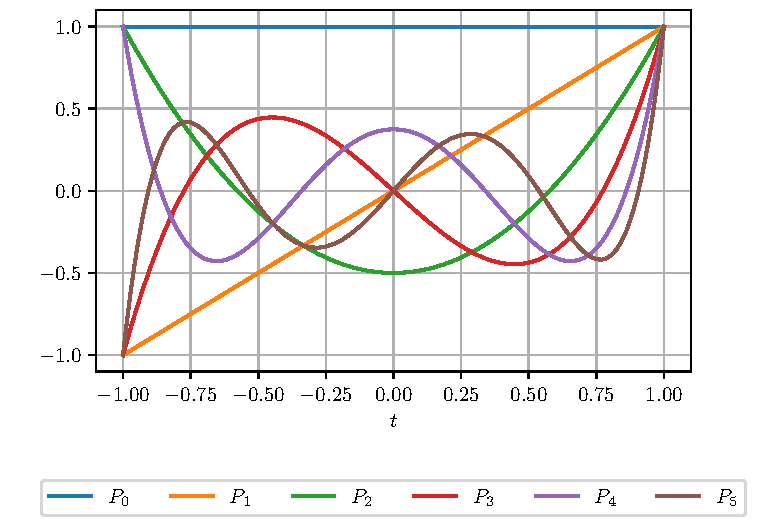
\includegraphics{./fig-legendre-polynomials.pdf}
\caption{Legendreove polynómy~$P_n(t)$ argumentu~$t \in [-1, 1]$ pre~$n = 0, 1, 
\dots, 5$.  V~úlohách súvisiacich s~tiažovým poľom zvykne parameter~$t$ 
reprezentovať napríklad funkciu~$\sin\varphi$ 
(rovnica~\ref{eq:pn_decomposition_formula} alebo vzťah~\ref{eq:vg_sh_no_norm} 
pre~$m = 0$) alebo funkciu~$\cos\psi$ (rovnica~\ref{eq:1l_legpol}).  Obrázok 
bol pripravený Zdrojovým
kódom~\ref{src:lp} z~Prílohy~\ref{app:lp}.}
\label{fig:lp}
\end{figure}

V~Kapitole~\ref{sec:sh_motivation} sme ukázali, že ľubovoľný vektor~$\vec r$
z~trojrozmerného karteziánskeho súradnicového systému je možné popísať pomocou
jednotkových vektorov~$\vec e_i$, $i = 1, 2, 3$.  Obdobne je možné pomocou
niektorých systémov funkcií popísať každú spojitú funkciu~$f(t)$ na intervale
$t \in [-1, 1]$.  Jeden z~takýchto systémov funkcií predstavujú práve
Legendreove polynómy~$P_n(t)$, $n = 0, 1, 2, \dots$  Rovnica
%
\begin{equation}
\label{eq:f_synthesis}
f(t) = \sum_{n = 0}^\infty \frac{2n + 1}{2} \, f_n \, P_n(t){,} \quad t \in 
[-1, 1]{,}
\end{equation}
%
umožňuje rozvinúť každú spojitú funkciu~$f(t)$ definovanú na intervale~$t \in 
[-1, 1]$ do radu Legendreových polynómov
pre ľubovoľné $t \in [-1, 1]$.  Vzťah~(\ref{eq:f_synthesis}) je možné vnímať aj
ako analógiu vzťahu~(\ref{eq:r_synthesis}), pričom~$f_n$ sú súradnice funkcie
$f(t)$ a~Legendreove polynómy~$P_n(t)$ plnia podobnú úlohu ako jednotkové
vektory~$\vec e_i$.  Koeficienty~$f_n$ sú dané skalárnym súčinom funkcií~$f(t)$
a~$P_n(t)$ (porovnaj so skalárnym súčinom~\ref{eq:r_analysis}),
%
\begin{equation}
\label{eq:f_analysis}
f_n = \int\limits_{-1}^1 f(t) \, P_n(t) \, \diff t{.}
\end{equation}
%
Dôkaz platnosti rovníc~(\ref{eq:f_synthesis}) a~(\ref{eq:f_analysis}) je možné 
nájsť napríklad vo \textcite{Freeden2009} 
a~v~\textcite{SansoGeoidDetermination}.

Pokračujme ďalej v~analógii s~jednotkovými vektormi.  Podobne ako skalárny 
súčin dvoch rôznych jednotkových vektorov je nulový 
(rovnica~\ref{eq:ei_orthogonality}), nulový je i~skalárny súčin dvoch rôznych 
Legendreovych polynómov,
%
\begin{equation}
\label{eq:lp_orthogonality}
\int\limits_{-1}^1 P_n(t) \, P_\ell(t) \, \diff t = 0{,} \quad n \neq \ell{.}
\end{equation}
%
Hovoríme preto, podobne ako v~súvislosti s~jednotkovými vektormi, že
\emph{Legendreove polynómy sú ortogonálne} na intervale $t \in [-1, 1].$
Rovnicu~(\ref{eq:lp_orthogonality}) možno zovšeobecniť doplnením prípadu~$n
= \ell$ \parencite[napríklad][]{Hobson},
%
\begin{equation}
\label{eq:lp_orthogonality_2}
\int\limits_{-1}^1 P_n(t) \, P_\ell(t) \, \diff t = \frac{2}{2n + 1} \, 
\delta_{n\ell}{.}
\end{equation}

Vo fyzikálnej geodézii sú rovnice~(\ref{eq:f_synthesis}) 
a~(\ref{eq:f_analysis}) využívané veľmi často a~v~istej miere sme sa s~nimi 
stretli už v~predchádzajúcej kapitole.  Nech~$f(t)$ je funkcia~$1 \slash \ell$ 
z~rovnice~(\ref{eq:1l_legpol}), $f(t) = 1 \slash \ell(t)$, $t = \cos\psi$, 
pričom~$r$ a~$r'$ sú konštanty, pre ktoré platí~$r > r'$ (pozri 
nerovnosť~\ref{eq:alpha_lt_1}).  Koeficienty~$f_n$ 
z~rovnice~(\ref{eq:f_analysis}) potom získame vzťahmi~(\ref{eq:1l_legpol}) 
a~(\ref{eq:lp_orthogonality_2}),
%
\begin{equation}
f_n = \frac{2}{2n + 1} \, \frac{1}{r'} \, \left( \frac{r'}{r} \right)^{n
+ 1}{.}
\end{equation}
%
Dosadením týchto koeficientov do vzťahu~(\ref{eq:f_synthesis}) získame pôvodný 
vzťah~(\ref{eq:1l_legpol}).  Hoci ide o~triviálny príklad, demonštruje 
rozvinutie funkcie do radu Legendreových polynómov.  Takéto rozvinutie je 
v~istom zmysle obdobné vyjadreniu vektora~$\vec r$ pomocou jednotkových 
vektorov~$\vec e_i$ z~Kapitoly~\ref{sec:sh_motivation}.  Tento rozvoj je 
v~mnohých situáciách výhodný, pretože môže napríklad zjednodušiť odvodenie.  
Napokon, najlepšie to demonštruje azda samotná 
Kapitola~\ref{sec:vg_sh_expansion}, v~ktorej sme funkciu~$1 \slash \ell$ 
rozvinuli do radu Legendreových polynómov (rovnica~\ref{eq:1l_legpol}) 
a~následne do radu Legendreových funkcií, čím sme získali 
vzťah~(\ref{eq:vg_sh_no_norm}).

V~niektorých aplikáciách fyzikálnej geodézie (napríklad 
Kapitola~\ref{sec:normal_gravity_in_sph_coords}) sa stretávame aj s~deriváciami 
Legendreových polynómov.  Deriváciu
%
\begin{equation}
P'_n(t) = \frac{\diff P_n(t)}{\diff t}
\end{equation}
%
môžeme vypočítať napríklad rekurentným vzťahom \parencite{Freeden2009}
%
\begin{equation}
P'_n(t) = n \, P_{n - 1}(t) + t \, P'_{n - 1}(t){.}
\end{equation}
%
Začiatočné hodnoty~$P'_0(t) = 0$ a $P'_1(t) = 1$ je možné získať deriváciou 
rovníc~(\ref{eq:p0_to_p5}) podľa premennej~$t$.  Častejšie než derivácie~$\diff 
P_n(t) \slash \diff t$ však potrebujeme poznať derivácie zložených 
funkcií~$\diff P_n(\sin\varphi) \slash \diff \varphi$ alebo~$\diff 
P_n(\cos\psi) \slash \diff \psi$.  Tie môžeme získať použitím nasledovných 
rekurentných vzťahov \parencite{Tscherning1976b},
%
\begin{align}
\label{eq:dlpsinphi_dphi}
\frac{\diff P_n(\sin\varphi)}{\diff \varphi} &= (2n - 1) \, \cos\varphi \, P_{n 
- 1}(\sin\varphi) + \frac{\diff P_{n - 2}(\sin\varphi)}{\diff \varphi}{,}\\
%
\label{eq:dlpcospsi_dpsi}
\frac{\diff P_n(\cos\psi)}{\diff \psi} &= -(2n - 1) \, \sin\psi \, P_{n 
- 1}(\cos\psi) + \frac{\diff P_{n - 2}(\cos\psi)}{\diff \psi}{.}
\end{align}
%
Začiatočné hodnoty získame opäť z~rovníc~(\ref{eq:p0_to_p5}) po uvážení~$t 
= \sin\varphi$ alebo~$t = \cos\psi$,
%
\begin{alignat}{2}
\frac{\diff P_0(\sin\varphi)}{\diff \varphi} &= 0{,} \quad \frac{\diff 
P_1(\sin\varphi)}{\diff \varphi} &&= \cos\varphi{,}\\
%
\frac{\diff P_0(\cos\psi)}{\diff \psi} &= 0{,} \quad \frac{\diff 
P_1(\cos\psi)}{\diff \psi} &&= -\sin\psi{.}
\end{alignat}

Legendreove polynómy majú mnoho zaujímavých a~užitočných vlastností.  Uveďme 
aspoň niektoré z~nich \parencite{Freeden2009},
%
\begin{alignat}{2}
\label{eq:pn_property1}
P_n(1) &= 1{,} && \quad n \geq 0{,}\\
%
\label{eq:pn_property2}
P_n(-t) &= (-1)^n \, P_n(t){,} && \quad n \geq 0{,}\\
%
\label{eq:pn_property3}
|P_n(t)| \leq P_n(1) &= 1{,} && \quad n \geq 0{,}\\
%
\int\limits_{-1}^{1} P_n(t) \, \diff t &= 0{,} && \quad n \geq 1{,}\\
%
\label{eq:pn_property4}
P_n'(1) &= \frac{n \, (n + 1)}{2}{,} && \quad n \geq 0{.}
\end{alignat}
%
Širokú škálu ďalších vlastností Legendreovych polynómov, ich derivácií či 
integrálov je možné nájsť napríklad v~prácach \textcite{Gradshteyn2007}, 
\textcite{Freeden2009} a~\textcite{Olver2010}.

Na záver pre úplnosť dodajme, že vzťahy~(\ref{eq:f_synthesis}) 
a~(\ref{eq:f_analysis}) možno aplikovať nielen na spojité funkcie, ale i~na 
širšiu množinu funkcií.  Podrobnosti možno nájsť napríklad v~prácach 
\textcite{Freeden2009} a~\textcite{Arfken2005}.






\section{Legendreove funkcie}
\label{sec:legendre_functions}

Dosadením Rodriguesovho vzorca~(\ref{eq:pn_rodrigues}) do~(\ref{eq:pnm_def})
získame vzťah pre Legendreove funkcie,
%
\begin{equation}
\label{eq:pnm_ferrer}
P_{nm}(t) = \frac{1}{2^n \, n!} (1 - t^2)^{ m \slash 2} \, \frac{\diff^{n + m}
(t^2 - 1)^n}{\diff t^{n + m}}{,}
\end{equation}
%
kde~$n = 0, 1, \dots$ a~$m = 0, 1, \dots n$.  Existuje tiež explicitný vzťah 
\parencite{Freeden2009}
%
\begin{equation}
P_{nm}(t) = \frac{1}{2^n}(1 - t^2)^{m \slash 2} \sum_{s = 0}^{\left\lfloor
\frac{n - m}{2} \right\rfloor} (-1)^s \, \frac{(2n - 2s)!}{s! \, (n - s)! \, (n
- m - 2s)!} \, t^{n - m - 2s}
\end{equation}
%
či mnoho rekurentných vzorcov, napríklad \parencite{Freeden2009}
%
\begin{equation}
\label{eq:pnm_recurrence}
P_{nm}(t) = \frac{2n - 1}{n - m} \, t \, P_{n - 1, m}(t) - \frac{n + m - 1}{n
- m} \, P_{n - 2, m}(t){,} \quad n \geq 2{.}
\end{equation}
%
Niekoľko prvých Legendreových funkcií má nasledovný tvar
(Obrázok~\ref{fig:lf}),
%
\begin{equation}
\label{eq:lf00_to_lf22}
\begin{split}
P_{0,0}(t) & = 1{,}\\
P_{1,0}(t) & = t{,}\\
P_{1,1}(t) & = \sqrt{1 - t^2}{,}\\
P_{2,0}(t) & = \frac{1}{2}(3t^2 - 1){,}\\
P_{2,1}(t) & = 3t \, \sqrt{1 - t^2}{,}\\
P_{2,2}(t) & = 3(1 - t^2){.}\\
\end{split}
\end{equation}

\begin{figure}[bt]
\centering
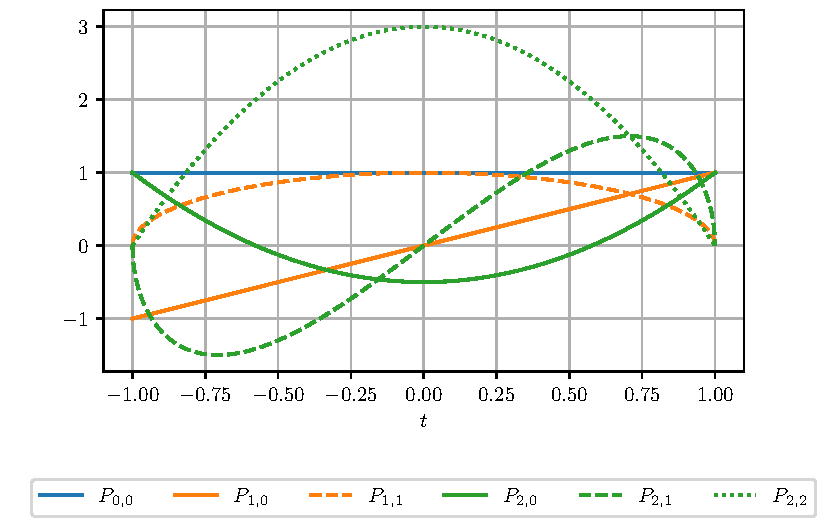
\includegraphics{./fig-legendre-functions.pdf}
\caption{Legendreove funkcie~$P_{nm}(t)$ argumentu~$t \in [-1, 1]$ pre~$n = 0, 
1, 2$ a~$m = 0, \dots, n$.  Symbol~$t$ môže označovať napríklad 
funkciu~$\sin\varphi$ (rovnica~\ref{eq:vg_sh_no_norm}).}
\label{fig:lf}
\end{figure}

Legendreove funkcie rôznych stupňov~$n$, $\ell$ a~rovnakého rádu~$m$ sú
ortogonálne \parencite{Freeden2009},
%
\begin{equation}
\label{eq:pnm_orthogonality}
\int\limits_{-1}^{1} P_{nm}(t) \, P_{\ell m}(t) \, \diff t = 0{,} \quad n \neq 
\ell{.}
\end{equation}
%
Pre dve Legendreove funkcie rovnakého stupňa a~rádu platí
%
\begin{equation}
\label{eq:pnm_times_pnm}
\int\limits_{-1}^{1} \left( P_{nm}(t) \right)^2 \, \diff t = \frac{2}{2n + 1} 
\, \frac{(n + m)!}{(n - m)!}{.}
\end{equation}

Legendreove funkcie vyhovujú diferenciálnej rovnici druhého rádu 
\parencite{SansoGeoidDetermination}
%
\begin{equation}
\label{eq:legfunc1_differential_equation}
(1 - t^2) \, \frac{\diff^2 P_{nm}(t)}{\diff t^2} - 2 \, t \, \frac{\diff 
P_{nm}(t)}{\diff t} + \left[ n \, (n + 1) - \frac{m^2}{1 - t^2} \right] \, 
P_{nm}(t) = 0{.}
\end{equation}
%
Rovnica~(\ref{eq:legfunc1_differential_equation}) sa nazýva \emph{Legendreova 
diferenciálna rovnica}.  Dosadením~$m = 0$ 
do~(\ref{eq:legfunc1_differential_equation}) získame diferenciálnu rovnicu 
druhého rádu pre Legendreove polynómy,
%
\begin{equation}
\label{eq:legpol_differential_equation}
(1 - t^2) \, \frac{\diff^2 P_n(t)}{\diff t^2} - 2 \, t \, \frac{\diff 
P_n(t)}{\diff t} + n \, (n + 1) \, P_n(t) = 0{.}
\end{equation}

Z~ďalších vlastností Legendreových funkcií spomeňme aspoň dve,
%
\begin{align}
\label{eq:pnm_symmetry}
P_{nm}(-t) &= (-1)^{n + m} \, P_{nm}(t){,}\\
%
P_{nm}(\pm1) &= 0{,} \quad m \neq 0{.}
\end{align}

Na numerický výpočet Legendreových funkcií sa zvyčajne používajú rekurentné 
vzťahy.  Ide však o~netriviálnu úlohu, obzvlášť pre vysoké stupne a~rády 
\parencite{Holmes2002a,Fukushima2012a,Ishioka2018}.  
Vlastnosť~(\ref{eq:pnm_symmetry}) je preto výhodná; ak potrebujeme vypočítať 
$P_{nm}(\sin\varphi)$ a~$P_{nm}(\sin(-\varphi))$, rekurentné vzťahy môžeme 
aplikovať iba na získanie jedného z~týchto členov a~druhý člen dopočítame 
vzťahom~(\ref{eq:pnm_symmetry}).  Rekurentné vzťahy pre derivácie Legendreových 
funkcií je možné nájsť napríklad v~prácach~\textcite{Tscherning1976b}, 
\textcite{Bosch2000}, \textcite{Holmes2002a}, \textcite{Freeden2009} 
a~\textcite{Fukushima2012b}.

Na záver dodajme, že v~niektorých vedných odboroch, napríklad vo fyzike či 
v~seizmológii, sa používa definícia Legendreových funkcií, ktorá obsahuje aj 
člen~$(-1)^m$ \parencite{Wieczorek2015,Olver2010},
%
\begin{equation}
\label{eq:pnm_cs_phase_factor}
\begin{split}
P_n^m(t) &= (-1)^m \, (1 - t^2)^{m \slash 2} \, \frac{\diff^m P_n(t)}{\diff 
t^m}\\
%
&= \frac{(-1)^m}{2^n \, n!} (1 - t^2)^{ m \slash 2} \, \frac{\diff^{n + m}
(t^2 - 1)^n}{\diff t^{n + m}}{.}
\end{split}
\end{equation}
%
Rád Legendreovej funkcie~$m$ sa v~takom prípade zvykne zapisovať do horného 
indexu.  Člen $(-1)^{m}$ sa nazýva \emph{Condonov--Shortleyho fázový faktor}.  
Medzi $P_{nm}(t)$ (rovnica~\ref{eq:pnm_ferrer}) a~$P_n^m(t)$ 
(rovnica~\ref{eq:pnm_cs_phase_factor}) platí vzťah
%
\begin{equation}
P_{nm}(t) = (-1)^m \, P_n^m(t){.}
\end{equation}
%
Ďalej budeme používať iba Legendreove funkcie $P_{nm}(t)$ definované 
vzťahom~(\ref{eq:pnm_ferrer}).




\section{Sférické harmonické funkcie}
\label{sec:spherical_harmonics}

Zaveďme v~rovnici~(\ref{eq:vg_sh_no_norm}) substitúciu pre členy, ktoré závisia
iba od uhlovej časti sférických súradníc,
%
\begin{equation}
\label{eq:ynk_no_norm}
Y_{nk}(\varphi, \lambda) = P_{n|k|}(\sin\varphi)
%
\begin{cases}
\cos(k\lambda){,}    &\text{ak} \quad k \geq 0{,}\\
\sin(|k|\lambda){,}  &\text{ak} \quad k < 0{,}\\
\end{cases}
\end{equation}
%
pričom $n = 0, 1, 2, \dots$ a~$k = -n, \dots, n$.  Funkcia $Y_{nk}(\varphi,
\lambda)$ sa nazýva \emph{plošná sférická harmonická funkcia stupňa $n$ a~rádu
$k$}.\footnote{Znamienko parametra~$k$ určuje, či plošná sférická harmonická 
funkcia~$Y_{nk}(\varphi, \lambda)$ obsahuje trigonometrickú 
funkciu~$\cos(k\lambda)$ alebo~$\sin(|k|\lambda)$.  Všimnime si, že 
v~rovnici~(\ref{eq:ynk_no_norm}) je rád Legendreovej 
funkcie~$P_{n|k|}(\sin\varphi)$ vždy nezáporný v~súlade s~definíciou 
Legendreových funkcií z~rovnice~(\ref{eq:pnm_def}).  V~ďalších častiach práce 
je potrebné rozlišovať medzi indexmi~$m = 0, 1, \dots, n$ (napríklad 
rovnica~\ref{eq:vg_sh_no_norm}) a~$k = -n, \dots, n$ (napríklad 
rovnica~\ref{eq:ynk_no_norm}).}

\begin{figure}[bt]
\centering
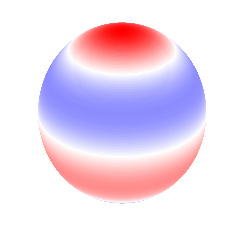
\includegraphics{./fig-spherical-harmonic-n3-k0.pdf}
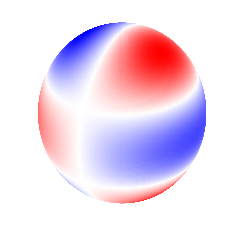
\includegraphics{./fig-spherical-harmonic-n3-k1.pdf}
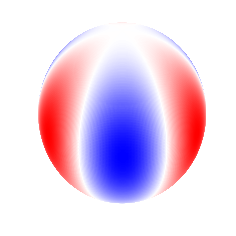
\includegraphics{./fig-spherical-harmonic-n3-k3.pdf}
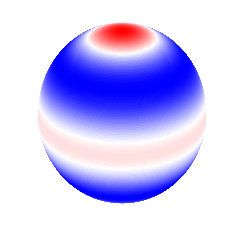
\includegraphics{./fig-spherical-harmonic-n4-k0.pdf}
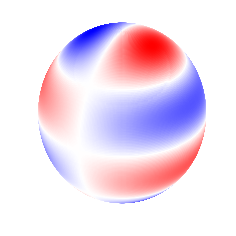
\includegraphics{./fig-spherical-harmonic-n4-k1.pdf}
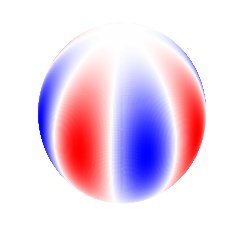
\includegraphics{./fig-spherical-harmonic-n4-k4.pdf}
\caption{Plošné sférické harmonické funkcie $Y_{nk}(\varphi, \lambda)$.
Záporné hodnoty sú zobrazené odtieňmi modrej farby, kladné hodnoty odtieňmi
červenej farby.  \textit{Vrchný rad} (zľava): $Y_{3,0}(\varphi, \lambda)$,
$Y_{3,1}(\varphi, \lambda)$, $Y_{3,3}(\varphi, \lambda)$.  \textit{Spodný rad}
(zľava): $Y_{4,0}(\varphi, \lambda)$, $Y_{4,1}(\varphi, \lambda)$,
$Y_{4,4}(\varphi, \lambda)$.  Obrázok bol pripravený Zdrojovým
kódom~\ref{src:ynk} z~Prílohy~\ref{app:sh}.}
\label{fig:sh}
\end{figure}

\begin{figure}[bt]
\centering
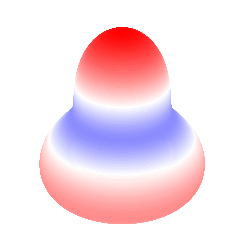
\includegraphics{./fig-spherical-harmonic-n3-k0-3d.pdf}
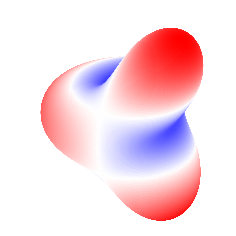
\includegraphics{./fig-spherical-harmonic-n3-k1-3d.pdf}
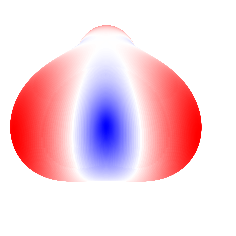
\includegraphics{./fig-spherical-harmonic-n3-k3-3d.pdf}
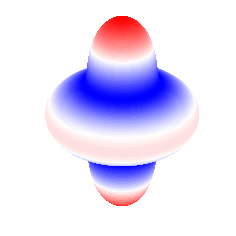
\includegraphics{./fig-spherical-harmonic-n4-k0-3d.pdf}
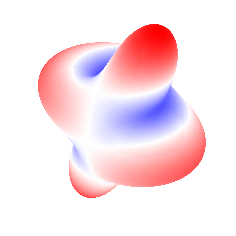
\includegraphics{./fig-spherical-harmonic-n4-k1-3d.pdf}
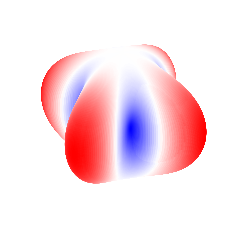
\includegraphics{./fig-spherical-harmonic-n4-k4-3d.pdf}
\caption{Plošné sférické harmonické funkcie $Y_{nk}(\varphi, \lambda)$
z~Obrázku~\ref{fig:sh} zobrazené odľahlosťou nadobúdanej hodnoty od jednotkovej
sféry.  Obrázok bol pripravený Zdrojovým kódom~\ref{src:ynk}
z~Prílohy~\ref{app:sh}.}
\label{fig:sh3d}
\end{figure}

Grafická reprezentácia sférických harmonických funkcií je uvedená na 
Obrázkoch~\ref{fig:sh} a~\ref{fig:sh3d}.  Z~obrázkov možno vypozorovať niekoľko 
vlastností sférických harmonických funkcií.
%
\begin{itemize}
\item Ak $k = 0$ (ľavý stĺpec na obrázkoch), sférické harmonické funkcie menia 
$n$-krát znamienko v~smere sférickej šírky a~nezávisia od sférickej dĺžky.  Obe 
vlastnosti môžu byť overené dosadením~$k = 0$ do rovnice~(\ref{eq:ynk_no_norm}) 
(pozri tiež Kapitolu~\ref{sec:legendre_polynomials} a~Obrázok~\ref{fig:lp}),
%
\begin{equation}
\label{eq:yn0}
Y_{n0}(\varphi, \lambda) = P_n(\sin\varphi){.}
\end{equation}
%
Funkcia~$Y_{n0}(\varphi, \lambda)$ je symetrická voči rovine rovníka, ak $n 
= 0, 2, 4, \dots$ a~nesymetrická, ak $n = 1, 3, 5, \dots$ (pozri 
rovnicu~\ref{eq:yn0} a~vlastnosti Legendreových polynómov 
v~Kapitole~\ref{sec:legendre_polynomials}). Funkcie~$Y_{n0}(\varphi, \lambda)$ 
sa nazývajú \emph{zonálne sférické harmonické funkcie}.

\item Ak $0 < |k| < n$ (prostredný stĺpec na obrázkoch), sférická harmonická 
funkcia mení znamienko s~oboma súradnicami.  V~smere sférickej šírky dochádza 
k~$n - |k|$ zmenám znamienka.  Počet $n - |k|$ vyplýva z~$|k|$-tej derivácie 
Legendreovho polynómu $P_n(\sin\varphi)$ (pozri rovnice~\ref{eq:pnm_def} 
a~\ref{eq:pnm_ferrer}).  Deriváciou polynómu sa znižuje jeho stupeň, a~teda aj 
počet možností meniť znamienko.  V~smere sférickej dĺžky sa znamienko mení 
$2|k|$-krát, čo vyplýva z~vlastností trigonometrických funkcií $\cos(k\lambda)$ 
a~$\sin(|k|\lambda)$.  Sférická harmonická funkcia rádu $0 < |k| < n$ má 
prívlastok \emph{teserálna}.

\item Ak $|k| = n$ (pravý stĺpec na obrázkoch), sférická harmonická funkcia 
mení znamienko $0$-krát v~smere sférickej šírky, pretože $n - |k| = n - n = 0$, 
a~$2|k|$-krát v~smere sférickej dĺžky.  Takáto funkcia sa nazýva 
\emph{sektorálna sférická harmonická funkcia}.
\end{itemize}

Podobne ako jednotkové vektory, Legendreove polynómy či Legendreove funkcie 
rovnakého rádu, i~sférické harmonické funkcie sú ortogonálne.  Táto vlastnosť 
vyplýva z~nulového skalárneho súčinu dvoch rôznych sférických harmonických 
funkcií,
%
\begin{equation}
\label{eq:ynk_no_norm_orthogonality}
\iint\limits_{\sigma} Y_{nk}(\varphi, \lambda) \, Y_{rs}(\varphi, \lambda) \, 
\diff \sigma = 0{,}
\end{equation}
%
pričom buď $n \neq r$ alebo $k \neq s$ alebo platia obe podmienky súčasne.  Pre
skalárny súčin dvoch rovnakých sférických harmonických funkcií platí vzťah
%
\begin{equation}
\label{eq:ynk_times_ynk}
\iint\limits_{\sigma} \left( Y_{nk}(\varphi, \lambda) \right)^2 \, \diff \sigma 
=
%
\dfrac{4\pi}{(2 - \delta_{k0}) \, (2n + 1)} \, \dfrac{(n + |k|)!}{(n
- |k|)!}{.}
\end{equation}
%
Overenie vzťahov~(\ref{eq:ynk_no_norm_orthogonality})
a~(\ref{eq:ynk_times_ynk}) ponecháme na čitateľa.  Je potrebné použiť
rovnice~(\ref{eq:pnm_orthogonality}), (\ref{eq:pnm_times_pnm}),
(\ref{eq:ynk_no_norm}) a~vypočítať integrály
%
\begin{equation}
\int\limits_{0}^{2\pi} \cos(k \lambda) \, \diff\lambda \quad \text{a} \quad
\int\limits_{0}^{2\pi} \sin(|k| \lambda) \, \diff\lambda{.}
\end{equation}
%
Vo vzťahoch~(\ref{eq:pnm_orthogonality}) a~(\ref{eq:pnm_times_pnm}) je potrebné
aplikovať zámenu integračnej premennej
%
\begin{equation}
\int\limits_{-1}^{1} P_{nm}(t) \, P_{rs}(t) \, \diff
t~= \int\limits_{-\frac{\pi}{2}}^{\frac{\pi}{2}} P_{nm}(\sin\varphi) \,
P_{rs}(\sin\varphi) \, \cos\varphi \, \diff \varphi{.}
\end{equation}


Nech $f(\varphi, \lambda)$ je funkcia na jednotkovej sfére $\sigma$ vyhovujúca 
nerovnosti
%
\begin{equation}
\label{eq:f_l2}
\iint\limits_\sigma \left( f(\varphi, \lambda) \right)^2 \, \diff \sigma 
< \infty{.}
\end{equation}
%
Podmienku~(\ref{eq:f_l2}) spĺňa napríklad každá spojitá funkcia na jednotkovej
sfére.  Každú takúto funkciu $f(\varphi, \lambda)$ možno rozvinúť do radu
sférických harmonických funkcií \parencite[napríklad][]{MoritzPhysicalGeodesy},
%
\begin{equation}
\label{eq:f_shs_no_norm}
f(\varphi, \lambda) = \sum_{n = 0}^\infty \sum_{k = -n}^n f_{nk} \,
Y_{nk}(\varphi, \lambda){.}
\end{equation}
%
Koeficienty $f_{nk}$ je možné získať nasledovne.  Vynásobme 
rovnicu~(\ref{eq:f_shs_no_norm}) sférickou harmonickou funkciou 
$Y_{rs}(\varphi, \lambda)$ a~následne rovnicu zintegrujme na jednotkovej sfére 
$\sigma$.  Použitím vzťahov~(\ref{eq:ynk_no_norm_orthogonality}) 
a~(\ref{eq:ynk_times_ynk}) získame hľadané koeficienty
%
\begin{equation}
\label{eq:f_sha_no_norm}
f_{nk} = \frac{(2 - \delta_{k0}) \, (2n + 1)}{4\pi} \, \frac{(n - |k|)!}{(n 
+ |k|)!} \, \iint\limits_{\sigma} f(\varphi, \lambda) \, Y_{nk}(\varphi, 
\lambda) \, \diff \sigma{.}
\end{equation}

Vidíme teda, že ak je splnená podmienka~(\ref{eq:f_l2}), potom 
funkciu~$f(\varphi, \lambda)$ možno rozložiť pomocou sférických harmonických 
funkcií na súradnice $f_{nk}$ (rovnica~\ref{eq:f_sha_no_norm}) a~následne ju 
spätne zrekonštruovať (vzťah~\ref{eq:f_shs_no_norm}).  V~priestore funkcií 
$f(\varphi, \lambda)$, ktoré sú definované na sfére a~spĺňajú 
podmienku~($\ref{eq:f_l2}$), plnia sférické harmonické funkcie $Y_{nk}(\varphi, 
\lambda)$ podobnú úlohu ako plnia jednotkové vektory $\vec e_i$ v~priestore 
trojrozmerných vektorov $\vec r$.  Funkcia $f(\varphi,\lambda)$ môže byť 
napríklad gravitačný či magnetický potenciál telesa na sfére, ktorá obopína 
celé teleso, topografia Zeme či inej planéty a~mnoho ďalších funkcií.  Každú 
takúto funkciu možno rozvinúť do vlastného radu sférických harmonických funkcií 
(vzťah~\ref{eq:f_shs_no_norm}), pričom každá funkcia bude mať vlastné súradnice 
$f_{nk}$, podobne ako každý vektor $\vec r$ má vlastné súradnice $r_i$.  
Všimnime si, že ak označíme
%
\begin{equation}
\label{eq:sh_norm}
N_{nk} = \sqrt{(2 - \delta_{k0}) (2n + 1) \, \frac{(n - |k|)!}{(n
+ |k|)!}}{,}
\end{equation}
%
potom vzťahy~(\ref{eq:f_sha_no_norm}) a~(\ref{eq:f_shs_no_norm}) sú totožné so
vzťahmi~(\ref{eq:vg_analysis}) a~(\ref{eq:vg_synthesis}) pre $r = 1$.



\section{Normovanie}
\label{sec:normalization}

V~praktických aplikáciách sa sférické harmonické funkcie zvyknú definovať tak, 
že sú vynásobené členom, ktorý závisí od sférického harmonického stupňa a~rádu.  
Tento člen sa nazýva \emph{norma} a~jeho použitím dostaneme \emph{normované 
sférické harmonické funkcie}.  Normovaním získame niektoré vlastnosti, ktoré sú 
výhodne z~teoretického aj z~praktického hľadiska.  Tieto vlastnosti budú 
podrobnejšie diskutované v~Kapitolách~\ref{sec:leg_sh_norm} 
a~\ref{sec:shc_norm}.  Existuje niekoľko typov noriem, napríklad Schmidtova 
polovičná norma, ortonormálna norma či úplná norma \parencite{SHTOOLS}.  
V~geodézii sa používa takmer výhradne úplná norma, preto sa budeme venovať iba 
jej.

\subsection{Legendreove funkcie a~sférické harmonické funkcie}
\label{sec:leg_sh_norm}

Pre skalárny súčin dvoch rovnakých jednotkových vektorov $\vec e_i$ platí 
vzťah~(\ref{eq:ei_unit_length}).  Z~teoretického aj z~praktického hľadiska by 
bolo výhodné, aby aj skalárny súčin dvoch rovnakých sférických harmonických 
funkcií bol rovný~$1$.  Túto vlastnosť možno zabezpečiť vynásobením 
Legendreových funkcií $P_{nm}(\sin\varphi)$ členom $N_{nk}$ 
(rovnica~\ref{eq:sh_norm}), ktorý nazývame \emph{úplná norma}.  Získame tým 
\emph{úplne normované Legendreove funkcie},
%
\begin{equation}
\bar{P}_{nm}(\sin\varphi) = N_{nm} \, P_{nm}(\sin\varphi){,} \quad  n = 0, 1, 
\dots,
\quad m = 0, 1, \dots, n{,}
\end{equation}
%
a~\emph{úplne normované sférické harmonické funkcie},
%
\begin{equation}
\label{eq:ynk_norm}
\begin{split}
\bar{Y}_{nk}(\varphi, \lambda) = N_{nk} \, Y_{nk}(\varphi, \lambda)
= \bar{P}_{n|k|}(\sin\varphi)
%
\begin{cases}
\cos(k\lambda){,}    &\text{ak} \quad k \geq 0{,}\\
\sin(|k|\lambda){,}  &\text{ak} \quad k < 0{,}
\end{cases}
&
%
\\
n = 0, 1, \dots, \quad k = -n, \dots, n{.}&
\end{split}
\end{equation}
%
Podobne ako v~súvislosti s~rovnicou~(\ref{eq:ynk_no_norm_orthogonality}), 
použitím normy~(\ref{eq:sh_norm}) možno dokázať rovnosť
%
\begin{equation}
\label{eq:ynk_norm_orthogonality}
\frac{1}{4\pi} \, \iint\limits_{\sigma} \bar{Y}_{nk}(\varphi, \lambda) \,
\bar{Y}_{rs}(\varphi, \lambda) \, \diff \sigma = \delta_{nr} \, \delta_{ks}{.}
\end{equation}
%
Skalárny súčin~(\ref{eq:ynk_norm_orthogonality}) dvoch rôznych úplne
normovaných sférických harmonických funkcií je teda rovný 0, zatiaľ čo skalárny
súčin dvoch rovnakých úplne normovaných sférických harmonických funkcií je
rovný $1$.

Vzťahy~(\ref{eq:f_shs_no_norm}) a~(\ref{eq:f_sha_no_norm}) potom nadobudnú tvar
%
\begin{align}
\label{eq:f_shs}
f(\varphi, \lambda) &= \sum_{n = 0}^\infty \sum_{k = -n}^n \bar{f}_{nk} \,
\bar{Y}_{nk}(\varphi, \lambda){,}\\
%
\label{eq:f_sha}
\bar{f}_{nk} &= \frac{1}{4\pi} \, \iint\limits_{\sigma} f(\varphi, \lambda) \,
\bar{Y}_{nk}(\varphi, \lambda) \, \diff \sigma{.}
\end{align}
%
Úplne normované sférické harmonické funkcie tiež umožňujú zapísať dekompozičný
teorém~(\ref{eq:pn_decomposition_formula}) v~tvare
\parencite{MoritzPhysicalGeodesy}
%
\begin{equation}
P_n(\cos\psi) = \frac{1}{2n + 1} \, \sum_{k = -n}^n \bar{Y}_{nk}(\varphi,
\lambda) \, \bar{Y}_{nk}(\varphi', \lambda')
\end{equation}
%
a~prevrátenú hodnotu vzdialenosti $1 \slash \ell$ 
z~rovnice~(\ref{eq:1l_legpol}) v~tvare
%
\begin{equation}
\label{eq:1l_sh}
\frac{1}{\ell} = \frac{1}{r'} \, \sum_{n = 0}^{\infty} \frac{1}{2n + 1} \, 
\left( \frac{r'}{r} \right)^{n + 1} \, \sum_{k = -n}^n \bar{Y}_{nk}(\varphi,
\lambda) \, \bar{Y}_{nk}(\varphi', \lambda'){.}
\end{equation}

Z~numerického hľadiska je výpočet nenormovaných Legendreových funkcií 
problematický, a~to už i~pre stupne a~rády presahujúce niekoľko stoviek.  
Dôvodom je ich pomerne rýchlo narastajúca hodnota, ktorá dokonca prekročí 
rozsah dvojitej presnosti.  \emph{Dvojitá presnosť} je v~súčasnosti 
najčastejšie používaný štandard na počítačovú reprezentáciu čísel s~pohyblivou 
desatinnou čiarkou.  Číslo väčšie ako horný rozsah dvojitej presnosti je 
v~dvojitej presnosti reprezentované nekonečnom.  Z~tohto dôvodu je 
z~praktického hľadiska výhodnejšie pracovať s~úplne normovanými Legendreovými 
funkciami.  Kvôli opísaným numerickým problémom sa však nepočíta zvlášť norma 
$N_{nm}$ a~zvlášť nenormovaná Legendreova funkcia $P_{nm}(\sin\varphi)$, ale 
počítajú sa priamo úplne normované Legendreove funkcie 
$\bar{P}_{nm}(\sin\varphi)$ pomocou upravených rekurentných vzťahov (pozri 
napríklad \cite{Holmes2002a} či \cite{Fukushima2012a}).



\subsection{Sférické harmonické koeficienty}
\label{sec:shc_norm}

Sférické harmonické koeficienty $C_{nm}$ a~$S_{nm}$ zo
vzťahu~(\ref{eq:vg_sh_no_norm}) sú zvyčajne normované dvakrát.  Prvá norma
zabezpečuje ich bezrozmernosť, druhá norma je potrebná v~dôsledku normovania 
sférických harmonických funkcií~(Kapitola~\ref{sec:leg_sh_norm}).

Fyzikálna jednotka koeficientov $C_{nm}$ a~$S_{nm}$
z~rovnice~(\ref{eq:vg_shc_no_norm}) je $\mathrm{m}^n \, \mathrm{kg}$ a~závisí 
od stupňa~$n$.  Je preto výhodne koeficienty normovať tak, aby boli
bezrozmerné.  Norma zaužívaná v~geodézii má tvar
%
\begin{equation}
\label{eq:cnm_snm_1st_norm}
\begin{rcases}
\tilde{C}_{nm}\\
\tilde{S}_{nm}
\end{rcases}
= \frac{1}{M \, R^n}
\begin{cases}
C_{nm}{,}\\
S_{nm}{,}
\end{cases}
\end{equation}
%
kde $M$ je hmotnosť telesa, ktoré generuje gravitačný potenciál a~$R$ je
polomer najmenšej sféry, v~ktorej sa nachádza celé teleso.  
Vzťah~(\ref{eq:vg_sh_no_norm})
potom prejde do tvaru
%
\begin{equation}
\label{eq:vg_sh_1st_norm}
V_\gidx(P) = \frac{GM}{R} \sum_{n = 0}^\infty \left( \frac{R}{r} \right)^{n
+ 1} \sum_{m = 0}^{n} \left( \tilde{C}_{nm} \, \cos(m\lambda) + \tilde{S}_{nm}
\, \sin(m\lambda)\right) \, P_{nm}(\sin\varphi){.}
\end{equation}

Ak sú sférické harmonické funkcie normované členom $N_{nk}$ 
(rovnica~\ref{eq:ynk_norm}), potom sférické harmonické koeficienty musia byť 
normou $N_{nk}$ vydelené, aby sa zachovala rovnosť vo 
vzťahoch~(\ref{eq:vg_sh_no_norm}) a~(\ref{eq:vg_sh_1st_norm}).  Druhá norma 
sférických harmonických koeficientov je preto daná nasledovne,
%
\begin{equation}
\label{eq:cnm_snm_2nd_norm}
\begin{rcases}
\bar{C}_{nm}\\
\bar{S}_{nm}
\end{rcases}
= \frac{1}{N_{nm}}
\begin{cases}
\tilde{C}_{nm}{,}\\
\tilde{S}_{nm}{.}
\end{cases}
\end{equation}
%
Sférický harmonický rozvoj~(\ref{eq:vg_sh_1st_norm}) následne prejde do tvaru
%
\begin{equation}
\label{eq:vg_sh_2nd_norm}
V_\gidx(P) = \frac{GM}{R} \sum_{n = 0}^\infty \left( \frac{R}{r} \right)^{n
+ 1} \sum_{m = 0}^{n} \left( \bar{C}_{nm} \, \cos(m\lambda) + \bar{S}_{nm} \,
\sin(m\lambda)\right) \, \bar{P}_{nm}(\sin\varphi){.}
\end{equation}
%
Ekvivalentný, no úspornejší zápis dosiahneme použitím substitúcie
$\bar{Y}_{nk}(\varphi, \lambda)$,
%
\begin{equation}
\label{eq:vg_sh_2nd_norm_ynk}
V_\gidx(P) = \frac{GM}{R} \sum_{n = 0}^\infty \left( \frac{R}{r} \right)^{n
+ 1} \sum_{k = -n}^{n} \bar{v}_{nk} \, \bar{Y}_{nk}(\varphi, \lambda){,}
\end{equation}
kde
%
\begin{equation}
\bar{v}_{nk} =
%
\begin{cases}
\bar{C}_{nk}{,}    &\text{ak} \quad k \geq 0{,}\\
\bar{S}_{n|k|}{,}  &\text{ak} \quad k < 0{.}\\
\end{cases}
\end{equation}
%
Koeficienty $\bar{C}_{nm}$ a~$\bar{S}_{nm}$, resp. $\bar{v}_{nk}$, sa nazývajú
\emph{úplne normované sférické harmonické koeficienty}.

Podobne ako úplne normované Legendreove funkcie, ani sférické
harmonické koeficienty sa nezvyknú počítať samostatne od normy.  Namiesto toho
sa vypočítajú úplne normované sférické harmonické funkcie
$\bar{Y}_{nk}(\varphi, \lambda)$ a~následne sa napríklad
vzťahom~(\ref{eq:f_sha}) priamo získajú úplne normované sférické harmonické
koeficienty.





% -----------------------------------------------------------------------------

\section{Fyzikálny význam niektorých sférických harmonických koeficientov}
\label{sec:physical_meaning_of_spherical_harmonic_coefficients}

Dosaďme $P_{0,0}(\sin\varphi)$ z~rovnice~(\ref{eq:lf00_to_lf22})
do rovnice~(\ref{eq:vg_shc_no_norm}) pre $n = 0$ a~$m = 0$,
%
\begin{equation}
\label{eq:c00_mass}
C_{0,0} = \iiint\limits_{\tau} \rho(Q) \, \diff \tau(Q) = M{.}
\end{equation}
%
Nenormovaný koeficient $C_{0,0}$ má teda fyzikálny význam, je rovný hmotnosti 
telesa~$M$.  Ak obmedzíme nekonečné rady~(\ref{eq:vg_sh_no_norm}), 
(\ref{eq:vg_sh_1st_norm}), (\ref{eq:vg_sh_2nd_norm}) či 
(\ref{eq:vg_sh_2nd_norm_ynk}) na maximálny stupeň $N = 0$, získame vzťah
%
\begin{equation}
\label{eq:vg_sh_0degree}
V_\gidx(P) = \frac{GM}{r}{.}
\end{equation}
%
Tento vzťah je identický s~rovnicou pre gravitačný potenciál hmotného 
bodu~(\ref{eq:vg_point_mass}) a~s~rovnicou pre gravitačný potenciál homogénnej 
gule v~bodoch mimo gule~(\ref{eq:vg_ball_out}).  Jedna z~možných interpretácií 
obmedzenia nekonečných rozvojov~(\ref{eq:vg_sh_no_norm}), 
(\ref{eq:vg_sh_1st_norm}), (\ref{eq:vg_sh_2nd_norm}) 
a~(\ref{eq:vg_sh_2nd_norm_ynk}) na maximálny stupeň $N = 0$ je teda taká, že 
získame gravitačný potenciál homogénnej gule, ktorá nahrádza skutočné teleso.

Vydeľme rovnicu~(\ref{eq:vg_shc_no_norm}) hmotnosťou $M$ a~zopakujme uvedený 
postup pre stupeň $n = 1$ a~rády $m = 0, 1$.  Po uvážení~(\ref{eq:sph2cart}) 
získame
%
\begin{equation}
\begin{split}
\frac{C_{1,0}}{M} &= \frac{1}{M} \iiint\limits_{\tau} \rho(Q) \, z' \, \diff 
\tau(Q) = z_\mathrm{c}{,}\\
\frac{C_{1,1}}{M} &= \frac{1}{M} \iiint\limits_{\tau} \rho(Q) \, x' \, \diff 
\tau(Q) = x_\mathrm{c}{,}\\
\frac{S_{1,1}}{M} &= \frac{1}{M} \iiint\limits_{\tau} \rho(Q) \, y' \, \diff 
\tau(Q) = y_\mathrm{c}{.}
\end{split}
\end{equation}
%
Súradnice $x_\mathrm{c}, y_\mathrm{c}, z_\mathrm{c}$ predstavujú posun začiatku 
súradnicového systému, v~ktorom vyjadrujeme polohu bodu~$P$ 
v~rovniciach~(\ref{eq:vg_sh_no_norm}), (\ref{eq:vg_sh_1st_norm}), 
(\ref{eq:vg_sh_2nd_norm}) a~(\ref{eq:vg_sh_2nd_norm_ynk}), voči ťažisku telesa.  
V~praktických aplikáciách pracujeme veľmi často v~geocentrickom súradnicovom 
systéme so začiatkom v~ťažisku Zeme, preto všetky koeficienty stupňa $n = 1$ sú 
často nulové, $C_{1,0} = C_{1,1} = S_{1,1} = 0$.

Je možné ukázať \parencite[napríklad][]{MoritzPhysicalGeodesy}, že koeficienty 
stupňa $n = 2$ súvisia s~momentom zotrvačnosti.  Zdá sa, že koeficienty 
stupňov~$n \geq 3$ už nemajú priamočiaru fyzikálnu interpretáciu.






% -----------------------------------------------------------------------------

\section{Aplikácie sférického harmonického rozvoja}
\label{sec:spherical_harmonics_applications}

V~tejto kapitole ukážeme dve aplikácie sférických harmonických rozvojov vo 
fyzikálnej geodézii: modelovanie vonkajšieho gravitačného 
poľa~(Kapitola~\ref{sec:sh_applications_gravity_field})
a~modelovanie topografie približne sférických 
telies~(Kapitola~\ref{sec:sh_applications_topography}).

\subsection{Gravitačné pole}
\label{sec:sh_applications_gravity_field}

Koeficienty $\bar{C}_{nm}$ a~$\bar{S}_{nm}$ je možné vypočítať napríklad 
z~obežnej dráhy umelej družice Zeme.  Tak ako Slnko ovplyvňuje dráhu planéty 
v~príklade z~Kapitoly~\ref{sec:newton_law}, podobne i~Zem vplýva na dráhu 
družice prostredníctvom svojho gravitačného poľa.  Tentokrát je ale situácia 
zložitejšia ako na Obrázku~\ref{fig:orbital_motion}, pretože družica obieha 
okolo Zeme vo výške približne $250$~-- $500$~km nad jej povrchom.  V~takejto 
bezprostrednej blízkosti Zeme sú priestorové variácie zemského gravitačného 
poľa dostatočne silné na to, aby ovplyvnili dráhu družice inak v~oblasti so 
silným gravitačným poľom (napríklad nad masívnymi pohoriami) a~inak 
v~oblastiach so slabším gravitačným poľom.  Skutočná dráha družice je preto 
komplikovaná priestorová krivka, ktorá reflektuje gravitačné pole v~danej 
oblasti, a~elipsa je len jej priblížením 
(Obrázok~\ref{fig:orbital_motion_real}).  Ak by sme teda poznali skutočnú dráhu 
družice, mali by sme byť schopní inverzným spôsobom vypočítať to pole, ktoré je 
príčinou neeliptickej dráhy.  Inými slovami, zo skutočnej dráhy družice je 
možné vypočítať sférické harmonické 
koeficienty~$\bar{C}_{nm}$~a~$\bar{S}_{nm}$.  
Koeficienty~$\bar{C}_{nm}$~a~$\bar{S}_{nm}$ je možné vypočítať i~z mnohých 
iných geodetických meraní, či už družicových alebo pozemných.  Podrobnejšie 
informácie o~pohybe družíc v~gravitačnom poli Zeme a~o~družicových misiách 
a~technikách je možné nájsť napríklad v~prácach 
\textcite{SeeberSatelliteGeodesy}, \textcite{MoritzPhysicalGeodesy}, 
\textcite{Kostelecky2008}, \textcite{Melicher2009} a~\textcite{Husar2017}.

\begin{figure}
\centering
\input{./fig-orbital-motion-real.pdf_tex}
\caption{Pohyb umelej družice Zeme.}
\label{fig:orbital_motion_real}
\end{figure}

V~Kapitole~\ref{sec:potential_theory} sme uviedli, že gravitačný potenciál 
obsahuje informáciu o~všetkých veličinách gravitačného poľa.  Zo 
vzťahu~(\ref{eq:vg_sh_2nd_norm}) je preto možné vyťažiť oveľa viac ako len 
informáciu o~gravitačnom potenciáli.  Napríklad aplikovaním operátora 
gradient~(\ref{eq:gradient_sph}) na gravitačný 
potenciál~(\ref{eq:vg_sh_2nd_norm}) možno získať prvky gravitačného zrýchlenia 
v~lokálnom karteziánskom súradnicovom systéme s~pohyblivým začiatkom 
$x^\mathrm{s}, y^\mathrm{s}, z^\mathrm{s}$ (Obrázok~\ref{fig:cart_sph}),
%
\begin{align}
\label{eq:vgx_sh}
\left.\frac{\partial V_\gidx}{\partial x^\mathrm{s}}\right|_P &= \frac{1}{r} \, 
\left.\frac{\partial V_\gidx}{\partial \varphi}\right|_P\nonumber\\
%
&= \frac{GM}{R^2} \sum_{n = 0}^\infty \left( \frac{R}{r} \right)^{n + 2} 
\sum_{m = 0}^{n} \left(
\bar{C}_{nm} \, \cos(m\lambda) + \bar{S}_{nm} \, \sin(m\lambda)\right) \,
\frac{\diff \bar{P}_{nm}(\sin\varphi)}{\diff \varphi}{,}\displaybreak[2]\\
%
\label{eq:vgy_sh}
\left.\frac{\partial V_\gidx}{\partial y^\mathrm{s}}\right|_P &= \frac{1}{r \, 
\cos\varphi} \, \left.\frac{\partial V_\gidx}{\partial 
\lambda}\right|_P\nonumber\\
%
&= \frac{GM}{R^2 \, \cos\varphi} \sum_{n = 0}^\infty \left( \frac{R}{r} 
\right)^{n + 2} \sum_{m = 0}^{n}\left(
\bar{S}_{nm} \, \cos(m\lambda) - \bar{C}_{nm} \, \sin(m\lambda)\right) \, m \,
\bar{P}_{nm}(\sin\varphi){,}\displaybreak[2]\\
%
\label{eq:vgz_sh}
\left.\frac{\partial V_\gidx}{\partial z^\mathrm{s}}\right|_P &= 
\left.\frac{\partial V_\gidx}{\partial r}\right|_P\nonumber\\
%
&= - \frac{GM}{R^2} \sum_{n = 0}^\infty (n + 1) \, \left( \frac{R}{r} 
\right)^{n + 2} \sum_{m = 0}^{n}
\left( \bar{C}_{nm} \, \cos(m\lambda) + \bar{S}_{nm} \, \sin(m\lambda)\right)
\, \bar{P}_{nm}(\sin\varphi){.}
\end{align}
%
Sférickými harmonickými rozvojmi teda môžeme vypočítať prakticky akúkoľvek 
veličinu gravitačného či tiažového poľa, od gravitačného potenciálu, cez 
gravitačné zrýchlenie až po zvislicové odchýlky či geoid.  
Rovnice~(\ref{eq:vgx_sh}) až~(\ref{eq:vgz_sh}) tiež prakticky demonštrujú 
výhodnosť vyjadrenia operátora gradient vo sférických súradniciach 
(rovnica~\ref{eq:gradient_sph}).  Priamy výpočet derivácií $\partial V_\gidx 
\slash \partial x^\mathrm{s}, \partial V_\gidx \slash \partial y^\mathrm{s}, 
\partial V_\gidx \slash \partial z^\mathrm{s}$ vzťahu~(\ref{eq:vg_sh_2nd_norm}) 
by bol náročný.

ICGEM (angl. \emph{International Centre for Global Earth Models}) je služba 
zriadená Medzinárodnou geodetickou asociáciou (angl.~\emph{International 
Association of Geodesy}, IAG).  Okrem iného je jej cieľom zbierať, archivovať 
a~poskytovať globálne modely gravitačného poľa Zeme, najčastejšie práve vo 
forme sférických harmonických koeficientov~$\bar{C}_{nm}$~a~$\bar{S}_{nm}$.  Na 
jej domovskej 
stránke\footnote{\label{fn:icgem_link}\url{http://icgem.gfz-potsdam.de/home}} 
je možné nájsť desiatky sád sférických harmonických koeficientov, ktoré boli 
získané z~rôznych dát a~rozličnými metódami výpočtu.  Dostupné sú aj časovo 
premenlivé modely zemského gravitačného poľa (pozri 
Kapitolu~\ref{sec:time_variable_gravity}).  Tieto modely zachytávajú časové 
variácie gravitačného poľa, ktoré sú spôsobené napríklad hydrologickými zmenami 
na regionálnej úrovni (napríklad Amazonský prales), presunom vodných más 
v~oceánoch, úbytkom ľadovcov v~Grónsku a~v~Antarktíde či zmeny spôsobené 
zemetraseniami \parencite{Wahr2007}.  ICGEM tiež poskytuje službu na výpočet 
vzťahu~(\ref{eq:vg_sh_2nd_norm}) či modely gravitačného poľa nebeských telies 
(napríklad Mars, Venuša, Mesiac či asteroidy Slnečnej sústavy).

Služba ICGEM poskytuje modely v~štandardizovanom tvare v~textových súboroch 
s~príponou~\texttt{gfc}.  V~Prílohe~\ref{app:gfc_file} je uvedená ukážka~modelu 
s~názvom EIGEN-6C4 \parencite{EIGEN-6C4}.  Na začiatku \texttt{gfc} súborov sú 
spravidla uvedené stručné informácie o~poskytovanom modeli, najmä mená autorov 
modelu, dáta a~metódy použité na jeho výpočet a~odkazy na relevantnú odbornú 
literatúru.  Riadky s~kľúčovými slovami \texttt{earth\_gravity\_constant} 
a~\texttt{radius} v~hlavičke súboru udávajú hodnoty geocentrickej gravitačnej 
konštanty~$GM$ a~referenčného polomeru~$R$, ktoré sú spojené s~daným modelom.  
V~rovnici~(\ref{eq:vg_sh_2nd_norm_ynk}) a~jej rôznych podobách musia byť 
použité práve tieto hodnoty.  Všimnime si, že koeficient $\bar{C}_{0,0}$ modelu 
EIGEN-6C4 má hodnotu~$1$.  Je to spôsobené tým, že nenormovaný 
koeficient~$C_{0,0}$ je rovný hmotnosti Zeme (rovnica~\ref{eq:c00_mass}), avšak 
po aplikovaní prvej a~druhej normy~(rovnice~\ref{eq:cnm_snm_1st_norm} 
a~\ref{eq:cnm_snm_2nd_norm}) nadobudne hodnotu~$1$.  Môžeme si tiež všimnúť, že 
všetky koeficienty stupňa~$n = 1$ sú nulové, teda začiatok súradnicového 
systému modelu EIGEN-6C4 je vložený do ťažiska Zeme (pozri 
Kapitolu~\ref{sec:physical_meaning_of_spherical_harmonic_coefficients}).

Sférické harmonické koeficienty gravitačného poľa Zeme sú v~súčasnosti dostupné
približne do stupňa $2190$.  Získavané sú väčšinou kombináciou družicových
meraní (približne do stupňa $250$ až $300$) a~detailných pozemných
gravimetrických meraní (približne do stupňa $720$ až $2190$).  Existujú tiež 
modely, ktoré popisujú zemské gravitačné pole do vyšších stupňov ako $2190$.  
Tieto vysoké harmonické stupne však nie sú založené na meraniach zemského 
gravitačného poľa, ale na modelovaní gravitačného účinku topografických hmôt 
\parencite[napríklad][]{Ince2020}.  \emph{Topografické 
hmoty}\label{def:topographic_masses} sú hmoty, ktoré sa nachádzajú medzi 
geoidom a~fyzickým povrchom Zeme.




\subsection{Topografia}
\label{sec:sh_applications_topography}

V~Kapitole~\ref{sec:spherical_harmonics} sme uviedli, že do radu sférických
harmonických funkcií je možné rozvinúť nielen gravitačný potenciál, ale každú
funkciu, ktorá spĺňa podmienku~(\ref{eq:f_l2}).  Rozviňme preto do stupňa~$N$ 
napríklad zemskú topografiu $H(\varphi, \lambda)$,
%
\begin{equation}
\label{eq:h_shs}
H(\varphi, \lambda) = \sum_{n = 0}^{N} \sum_{k = -n}^n \bar{h}_{nk} \,
\bar{Y}_{nk}(\varphi, \lambda){.}
\end{equation}
%
Obrázok~\ref{fig:shs_h} znázorňuje vplyv parametra~$N$ na priestorové 
rozlíšenie funkcie $H(\varphi, \lambda)$.  Koeficienty~$\bar{h}_{nk}$ boli 
prevzaté z~modelu~DTM2006.0 \parencite{DTM2006}.  Hoci všetky tri mapy sú 
vypočítané s~rovnakým vzorkovaním ($0.25^{\circ}$ vo sférickej šírke a~dĺžke), 
miera detailu stúpa od vrchnej mapy smerom nadol.  Spôsobené je to tým, že 
maximálny stupeň~$N$, ktorý udáva priestorové rozlíšenie funkcie 
$H(\varphi,\lambda)$, narastá postupne od~$30$ cez~$90$ až do~$360$.  Odhad 
veľkosti najmenšieho priestorového prvku, ktorý môže byť reprezentovaný 
sférickým harmonickým rozvojom do stupňa~$N$, je možné získať vzťahom 
\parencite{Barthelmes2013}
%
\begin{equation}
l_{\min}(N) = \frac{\pi \, R}{N}{,}
\end{equation}
%
kde $l_{\min}$ je sférická vzdialenosť v~dĺžkových jednotkách na sfére 
s~polomerom $R$.  Zvyšovaním maximálneho stupňa $N$ teda zvyšujeme priestorovú 
podrobnosť (rozlíšenie) funkcie $H(\varphi, \lambda)$.

\begin{figure}
\centering
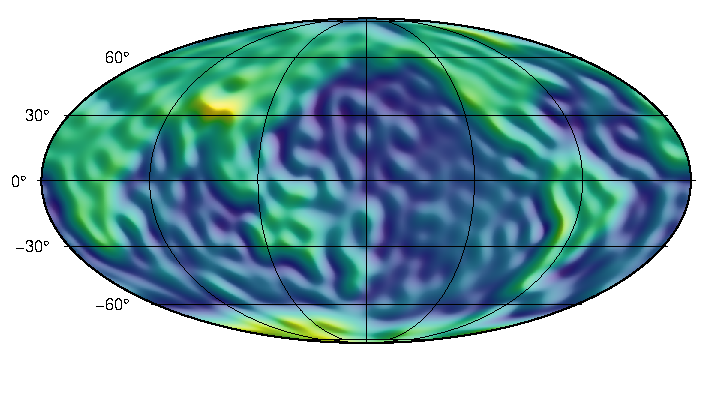
\includegraphics{./fig-h-shs-nmax30.pdf}
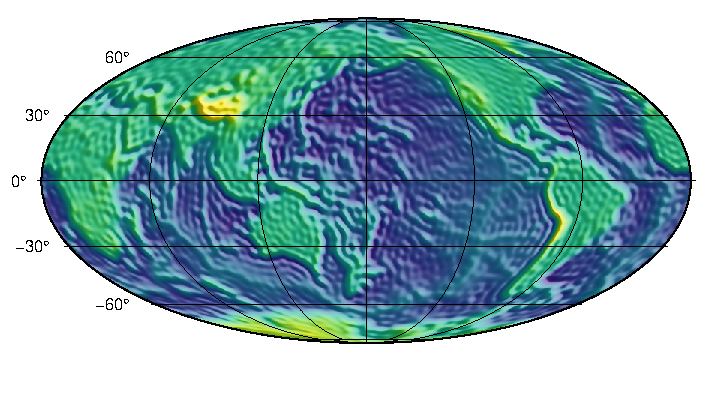
\includegraphics{./fig-h-shs-nmax90.pdf}
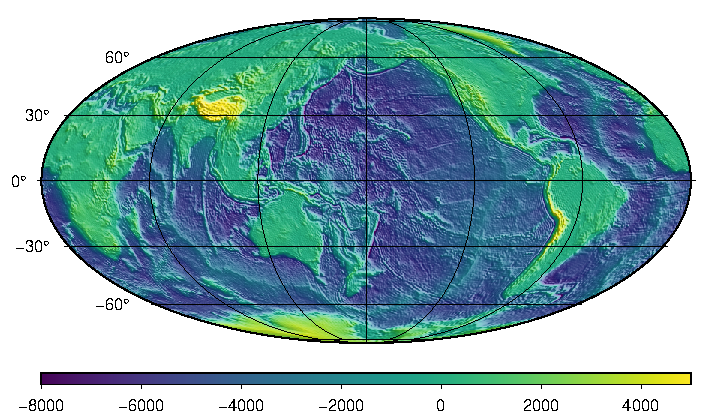
\includegraphics{./fig-h-shs-nmax360.pdf}
\caption{Sférický harmonický rozvoj zemskej topografie (jednotky~m) do 
stupňov~$N = 30$ (vrchná mapa), $90$~ (prostredná mapa) a~$360$~(spodná mapa).  
Výpočet bol uskutočnený Zdrojovým kódom~\ref{src:h_shs} 
z~Prílohy~\ref{app:shs_topography}.}
\label{fig:shs_h}
\end{figure}

Okrem modelu~DTM2006.0 je voľne prístupný aj model Earth2014 
\parencite{Hirt2015}.  Earth2014 je kolekcia modelov zemskej topografie 
v~rozličných variantoch, napríklad so zohľadnením výšky ľadovcov či s~uvážením 
alebo bez uváženia batymetrie.  Model DTM2006.0 je dostupný do stupňa~$2190$.  
Maximálny stupeň modelu Earth2014 je~$10\, 800$.

Zo sférických harmonických modelov topografie nebeských telies spomeňme aspoň 
model zemského Mesiaca do stupňa~2600 \parencite{Wieczorek2015} a~model 
asteroidu~Eros do stupňa~24 \parencite{Zuber2000}.





% -----------------------------------------------------------------------------

\section{Konvergencia sférického harmonického rozvoja na povrchu Zeme}
\label{sec:convergence_of_spherical_harmonics}

Pred rozvinutím generickej funkcie pre Legendreove polynómy do Maclaurinovho 
radu (vzťah~\ref{eq:maclaurin_series_of_generic_function}) sme vyslovili 
predpoklad $\frac{r'}{r} < 1$ (nerovnosť~\ref{eq:alpha_lt_1}).  Bez splnenia 
tejto podmienky rad~(\ref{eq:maclaurin_series_of_generic_function}) nemusí 
konvergovať.  V~takom prípade nie je možné pokračovať v~odvodení 
z~Kapitoly~\ref{sec:vg_sh_expansion}, pretože zámena poradia integrácie 
a~sumácie nie je možná.  Na získanie vzťahu~(\ref{eq:vg_sh_no_norm}) sme preto 
museli predpokladať, že podmienka $\frac{r'}{r} < 1$ je splnená.

\begin{figure}
\centering
\input{./fig-spherical-harmonics-convergence.pdf_tex}
\caption{Sférický harmonický rad~(\ref{eq:vg_sh_no_norm}) konverguje rovnomerne 
a~absolútne vo vonkajšom priestore sféry konvergencie.  Svetlosivá farba 
označuje oblasť, v~ktorej nie je zaručená konvergencia.  Tmavosivá farba 
predstavuje hmoty telesa, ktoré generuje gravitačné pole.  V~tejto oblasti 
rad~(\ref{eq:vg_sh_no_norm}) nepopisuje skutočný gravitačný potenciál.}
\label{fig:spherical_harmonics_convergence}
\end{figure}

Nerovnosť $\frac{r'}{r} < 1$ môžeme prepísať do tvaru $r > r'$.  Táto
nerovnosť je splnená pre \emph{všetky} diferenciálne elementy $\diff \tau(r',
\varphi', \lambda')$ iba vtedy, ak pre sprievodič $r$ výpočtového bodu $P(r,
\varphi, \lambda)$ platí
%
\begin{equation}
\label{eq:spherical_harmonic_convergence}
r > \max(r') = R{,}
\end{equation}
%
kde $R$ je sprievodič najvzdialenejšieho diferenciálneho elementu $\diff\tau$ 
od začiatku súradnicového systému.  Sféra s~polomerom $R$ sa nazýva sféra 
konvergencie \parencite{Hotine} 
(Obrázok~\ref{fig:spherical_harmonics_convergence}).  Vo vonkajšom priestore 
sféry konvergencie rad~(\ref{eq:vg_sh_no_norm}) konverguje rovnomerne 
a~absolútne.  Na tejto sfére ani v~jej vnútri konvergencia zaručená nie je.

Nanešťastie, celý povrch Zeme sa nachádza v~oblasti, v~ktorej sférický 
harmonický rozvoj gravitačného potenciálu nemusí konvergovať.  Našťastie, zdá 
sa, že otázka konvergencie, resp. divergencie radu~(\ref{eq:vg_sh_no_norm}) nie 
je v~súčasnosti z~praktického hľadiska relevantná pre nízke až stredné stupne 
a~svoju závažnosť nadobúda približne až od stupňa $10{,}800$ 
\parencite{Hirt2016,Rexer2017}.

Konvergencia radu sférických harmonických funkcií na povrchu Zeme je často 
diskutovanou témou geodetickej literatúry 
\parencite{Hotine,Borre_chapter4,MoritzAdvancedGeodesy,Sjoberg1980,Jekeli1983,SansoGeoidDetermination}.  
Dodajme, že funkcia~$1 \slash \ell$ môže byť rozvinutá do radu Legendreových 
polynómov a~do radu sférických harmonických funkcií aj pre~$r < r'$ 
\parencite[napríklad][]{Martinec1998,MoritzPhysicalGeodesy}.  Získame tým 
rozvoje, ktoré sú formálne podobné radom~(\ref{eq:1l_legpol}) 
a~(\ref{eq:1l_sh}).  Týmto spôsobom je možné odvodiť iný typ sférického 
harmonického rozvoja gravitačného potenciálu, ktorý je konvergentný aj pre~$r 
< R$, ak je v~tejto oblasti gravitačný potenciál harmonický.  V~literatúre sa 
preto rozlišuje medzi vonkajšími (podmienka~$r > R$) a~vnútornými priestorovými 
sférickými harmonickými funkciami ($r < R$).  Vonkajšie a~vnútorné rozvoje sa 
zvyknú aj kombinovať, vďaka čomu je možné získať konvergentný sférický 
harmonický rozvoj gravitačného potenciálu aj v~oblastiach so sprievodičom~$r 
< R$, a~to dokonca aj~vo vnútri Zeme 
\parencite[napríklad][]{Sjoberg1977,Jekeli1983,Grafarend1993,Wang1997,Martinec1998,Wang2013}.





% -----------------------------------------------------------------------------

\chapter{Sféroidický harmonický rozvoj}
\label{sec:spheroidal_harmonics_chapter}

Fyzikálna geodézia skúma gravitačné polia objektov rozmanitých tvarov.  Často 
pracujeme napríklad so sploštenými telesami, či už v~súvislosti so Zemou alebo 
s~mnohými asteroidmi Slnečnej sústavy (napríklad Eros, Castalia či Bennu; pozri 
\cite{Garmier2001}, \cite{Hu2015}, \cite{Sebera2016} či \cite{Reimond2016}).  
Ak by sme rozvinuli gravitačný potenciál týchto telies do sférického 
harmonického radu~(\ref{eq:vg_sh_no_norm}), oblasť možnej divergencie 
v~bezprostrednej blízkosti telesa môže byť rozsiahla (pozri 
Kapitolu~\ref{sec:convergence_of_spherical_harmonics}).  V~takýchto situáciách 
je výhodnejšie nerozvíjať gravitačný potenciál do radu harmonických funkcií vo 
sférických súradniciach, ale v~súradniciach, ktoré sú akýmsi spôsobom 
prirodzenejšie pre sploštené telesá.  Použité môžu byť napríklad 
\emph{redukované elipsoidické súradnice}, ktoré vedú ku \emph{sféroidickému 
harmonickému rozvoju} gravitačného potenciálu.  Prívlastok \emph{sféroidický} 
označuje, že harmonický rozvoj je vztiahnutý ku sféroidu, v~tomto prípade 
k~dvojosovému elipsoidu.  Hoci dvojosový elipsoid môže byť sploštený buď na 
póloch alebo na rovníku, pre modelovanie gravitačného poľa Zeme má praktické 
využitie takmer výlučne len prvý z~nich.  Ďalej sa preto budeme venovať iba 
elipsoidom, ktoré sú sploštené na póloch.  Výhodou sféroidického harmonického 
rozvoja je spravidla väčšia oblasť konvergencie harmonického radu v~porovnaní 
so sférickým rozvojom (pozri 
Obrázok~\ref{fig:spheroidal_harmonics_convergence}).

V~tejto kapitole popíšeme redukované elipsoidické súradnice 
(Kapitola~\ref{sec:reduced_ell_coords}), vyjadríme v~nich Laplaceovu rovnicu 
(Kapitola~\ref{sec:laplace_in_reduced_ell_coords}), predstavíme sféroidické 
harmonické funkcie (Kapitola~\ref{sec:spheroidal_harmonics}) a~na záver 
rozvinieme gravitačný potenciál do sféroidického harmonického radu 
(Kapitola~\ref{sec:spheroidal_harmonic_expansion}).  Kvôli náročnosti nebudeme 
odvádzať sféroidické harmonické funkcie tak podrobne ako sme odvodili sférické 
harmonické funkcie v~Kapitole~\ref{sec:spherical_harmonic_expansion}.  Namiesto 
toho sa budeme snažiť prirovnávať diskutované témy k~problematike známej už 
z~Kapitoly~\ref{sec:spherical_harmonic_expansion}.  Získané poznatky potom 
využijeme v~Kapitole~\ref{sec:normal_gravity_field}, v~ktorej je študované 
gravitačné a~tiažové pole s~konštantným tiažovým potenciálom na povrchu 
dvojosového elipsoidu.

\begin{figure}
\centering
\input{./fig-spheroidal-harmonics-convergence.pdf_tex}
\caption{Sféra a~dvojosový elipsoid konvergencie harmonických 
radov~(\ref{eq:vg_sh_no_norm}) a~(\ref{eq:vg_spheroidalh_2nd_norm_ynk}).  Oba 
rady konvergujú vo vonkajšom priestore svojej plochy konvergencie, no v~jej 
vnútri ich konvergencia zaručená nie je.  Oblasť konvergencie sféroidického 
harmonického radu je tak väčšia o~vyšrafovanú oblasť.}
\label{fig:spheroidal_harmonics_convergence}
\end{figure}


\section{Redukované elipsoidické súradnice}
\label{sec:reduced_ell_coords}

Nech je daný dvojosový referenčný elipsoid s~dĺžkou hlavnej polosi $a$ 
a~s~dĺžkou vedľajšej polosi $b$.  Parametre~$a$ a~$b$ sú volené tak, aby vhodne 
aproximovali tvar telesa, napríklad v~zmysle metódy najmenších štvorcov.  
Zaveďme ďalej pojem \emph{lineárna excentricita}~$E$.  Parameter~$E$ označuje 
vzdialenosť medzi stredom elipsy, ktorá vznikne meridiánovým rezom elipsoidu, 
a jedným z~jej ohnísk (Obrázok~\ref{fig:reduced_ell_coords}).  Z~definície 
elipsy vyplýva, že lineárna excentricita je daná vzťahom
%
\begin{equation}
\label{eq:linear_eccentricity}
E = \sqrt{a^2 - b^2}{.}
\end{equation}

Polohu ľubovoľného bodu~$P$, ktorý sa nachádza na referenčnom elipsoide alebo 
nad ním, možno vyjadriť pomocou redukovaných elipsoidických súradníc $u, \beta, 
\lambda$ (Obrázok~\ref{fig:reduced_ell_coords}).  Symbol $u$ označuje malú 
polos konfokálneho elipsoidu, ktorý prechádza bodom~$P$.  \emph{Konfokálny 
elipsoid} je taký elipsoid, ktorý má rovnakú lineárnu excentricitu~$E$ ako 
referenčný elipsoid.  Ak sa bod~$P$ nachádza na referenčnom elipsoide, potom~$u 
= b$.  Symbol $\beta$ predstavuje redukovanú elipsoidickú šírku.  Redukovaná 
elipsoidická dĺžka $\lambda$ je definovaná rovnako ako sférická dĺžka~$\lambda$ 
(pozri Obrázok~\ref{fig:cart_sph}).

\begin{figure}
\centering
\input{./fig-reduced-ell-coords.pdf_tex}
\caption{Redukované elipsoidické súradnice $u$ a~$\beta$ bodu $P$ vyjadrené 
pomocou referenčného elipsoidu s~hlavnou polosou~$a$ a~vedľajšou polosou~$b$.}
\label{fig:reduced_ell_coords}
\end{figure}

Jednoduchým spôsobom možno overiť, že medzi redukovanými elipsoidickými 
súradnicami a~karteziánskymi súradnicami platia nasledovné vzťahy,
%
\begin{equation}
\label{eq:ellred2cart}
\begin{split}
x &= \sqrt{u^2 + E^2} \, \cos\beta \, \cos\lambda{,}\\
y &= \sqrt{u^2 + E^2} \, \cos\beta \, \sin\lambda{,}\\
z &= u \, \sin\beta{,}
\end{split}
\end{equation}
%
kde $\sqrt{u^2 + E^2}$ je dĺžka hlavnej polosi konfokálneho elipsoidu.  Ak $E 
= 0$, teda ak referenčný elipsoid nie je sploštený, potom 
vzťahy~(\ref{eq:ellred2cart}) majú rovnaký tvar ako transformácia sférických 
súradníc na karteziánske súradnice~(\ref{eq:sph2cart}).  Pre transformáciu 
karteziánskych súradníc~$x, y, z$ na redukované elipsoidické súradnice~$u, 
\beta, \lambda$ pozri napríklad \textcite{MoritzPhysicalGeodesy}.



\section{Laplaceova rovnica v~redukovaných elipsoidických súradniciach}
\label{sec:laplace_in_reduced_ell_coords}

Z~podobných dôvodov ako v~Kapitole~\ref{sec:laplace_equation_sph} potrebujeme 
vyjadriť operátor gradient a~Laplaceov operátor aj v~systéme redukovaných 
elipsoidických súradníc.  Príslušné vzťahy nájdeme postupom uvedeným 
v~Prílohách~\ref{app:gradient_in_orthogonal_coordinates} 
a~\ref{app:laplace_in_orthogonal_coordinates}.

V~súlade s~Prílohou~\ref{app:gradient_in_orthogonal_coordinates} definujme 
vektory (pozri vzťah~\ref{eq:xi1xi2xi3_vectors})
%
\begin{equation}
\label{eq:eu_ebeta_elon}
\hat{\vec e}_1^\mathrm{r} = \frac{\partial \vec r(\beta, \lambda, u)}{\partial 
\beta}{,}
%
\quad
%
\hat{\vec e}_2^\mathrm{r} = \frac{\partial \vec r(\beta, \lambda, u)}{\partial 
\lambda}{,}
%
\quad
%
\hat{\vec e}_3^\mathrm{r} = \frac{\partial \vec r(\beta, \lambda, u)}{\partial 
u}{,}
%
\end{equation}
%
kde
%
\begin{equation}
\vec r =
%
\begin{bmatrix}
x(\beta, \lambda, u)\\
y(\beta, \lambda, u)\\
z(\beta, u)
\end{bmatrix}
{.}
%
\end{equation}
%
Funkcie $x(\beta, \lambda, u)$, $y(\beta, \lambda, u)$, $z(\beta, u)$ sú dané 
vzťahmi~(\ref{eq:ellred2cart}).  Začiatok a~smery vektorov~$\hat{\vec 
e}_i^\mathrm{r}$, $i = 1, 2, 3$, definujú lokálny karteziánsky súradnicový 
systém~$x^\mathrm{r}, y^\mathrm{r}, z^\mathrm{r}$ s~pohyblivým 
začiatkom~v~bode~$P$.  Os~$z^\mathrm{r}$ je daná smerom vonkajšej normály ku 
konfokálnemu elipsoidu v~bode~$P$.  Os~$x^\mathrm{r}$ leží v~dotykovej rovine 
ku konfokálnemu elipsoidu a~smeruje na sever.  Os~$y^\mathrm{r}$ dotvára 
pravouhlý \emph{ľavotočivý} súradnicový systém.
%
Pomocou rovníc~(\ref{eq:ellred2cart}) a~(\ref{eq:eu_ebeta_elon}) možno 
jednoducho ukázať, že pre $\| \hat{\vec e}_i^\mathrm{r} \|$, $i = 1, 2, 3$, 
platí
%
\begin{equation}
\label{eq:ei_reduced_ell_magnitudes}
\begin{split}
\| \hat{\vec e}_1^\mathrm{r} \| &= \sqrt{u^2 + E^2 \, \sin^2\beta}{,}\\
%
\| \hat{\vec e}_2^\mathrm{r} \| &= \sqrt{ u^2 + E^2} \, \cos\beta{,}\\
%
\| \hat{\vec e}_3^\mathrm{r} \| &= \sqrt{\frac{u^2 + E^2 \, \sin^2\beta}{u^2 
+ E^2}}{.}
\end{split}
\end{equation}

Kombináciou rovníc~(\ref{eq:grad_orthogonal_system}) 
a~(\ref{eq:ei_reduced_ell_magnitudes}) získame operátor gradient v~redukovaných 
elipsoidických súradniciach,
%
\begin{align}
\label{eq:gradient_red_ell}
\nabla f = \grad f &= \vec e_1^\mathrm{r} \, \frac{1}{\sqrt{u^2 + E^2 \, 
\sin^2\beta}} \, \frac{\partial f}{\partial \beta} + \vec e_2^\mathrm{r} \, 
\frac{1}{\sqrt{u^2 + E^2} \, \cos\beta} \, \frac{\partial f}{\partial \lambda} 
+ \vec e_3^\mathrm{r} \, \sqrt{\frac{u^2 + E^2}{u^2 + E^2 \, \sin^2\beta}} \, 
\frac{\partial f}{\partial u}\nonumber\displaybreak[2]\\
%
&=
%
\begin{bmatrix}
\dfrac{1}{\sqrt{u^2 + E^2 \, \sin^2\beta}} \, \dfrac{\partial f}{\partial 
\beta}\\[2ex]
\dfrac{1}{\sqrt{u^2 + E^2} \, \cos\beta} \, \dfrac{\partial f}{\partial 
\lambda}\\[2ex]
\sqrt{\dfrac{u^2 + E^2}{u^2 + E^2 \, \sin^2\beta}} \, \dfrac{\partial 
f}{\partial u}
\end{bmatrix}
{,}
\end{align}
%
kde
%
\begin{equation}
\vec e_i^\mathrm{r} = \frac{\hat{\vec e}_i^\mathrm{r}}{\| \hat{\vec 
e}_i^\mathrm{r} \|}{,} \quad i = 1, 2, 3{,}
\end{equation}
%
sú jednotkové vektory v~smere osí~$x^\mathrm{r}, y^\mathrm{r}, z^\mathrm{r}$.

Laplaceovu rovnicu pre gravitačný potenciál dostaneme 
vzťahmi~(\ref{eq:ei_reduced_ell_magnitudes}) 
a~(\ref{eq:laplace_orthogonal_system_final_2})
\parencite{MoritzPhysicalGeodesy},
%
\begin{equation}
\label{eq:vg_laplace_ellred}
(u^2 + E^2) \, \frac{\partial^2 V_\gidx}{\partial u^2} + 2u \, \frac{\partial 
V_\gidx}{\partial u} +  \frac{\partial^2 V_\gidx}{\partial\beta^2} - \tan\beta 
\, \frac{\partial V_\gidx}{\partial \beta} + \frac{u^2 + E^2 \, 
\sin^2\beta}{(u^2 + E^2) \, \cos^2\beta} \, \frac{\partial^2 V_\gidx}{\partial 
\lambda^2} = 0{.}
\end{equation}



\section{Sféroidické harmonické funkcie}
\label{sec:spheroidal_harmonics}

V~Kapitole~\ref{sec:vg_sh_expansion} sme uviedli, že rozvoj gravitačného 
potenciálu do radu sférických harmonických funkcií~(rovnica 
\ref{eq:vg_sh_no_norm}) môžeme získať aj riešením Laplaceovej diferenciálnej 
rovnice vo sférických súradniciach~(rovnica~\ref{eq:vg_laplace_sph}) metódou 
separácie premenných.  Cieľom takéhoto prístupu je nájsť tri funkcie, 
$f_{\mathrm{s}}(r)$, $g_{\mathrm{s}}(\varphi)$ a $h_{\mathrm{s}}(\lambda)$.  Je 
možne ukázať, že tieto funkcie majú tvar (porovnaj 
s~rovnicou~\ref{eq:vg_sh_no_norm})
%
\begin{align}
\label{eq:fs}
f_{\mathrm{s}}(r) &= \dfrac{1}{r^{n + 1}}{,}\\
%
\label{eq:gs}
g_{\mathrm{s}}(\varphi) &= P_{nm}(\sin\varphi){,}\\
%
\label{eq:hs}
h_{\mathrm{s}}(\lambda) &=
%
\begin{cases}
\cos(m\,\lambda){,}\\
\sin(m\,\lambda){,}
\end{cases}
\end{align}
%
kde $n = 0, 1, 2, \dots$ a~$m = 0, 1, \dots, n$.\footnote{Funkcia 
$f_{\mathrm{s}}(r)$ môže mať aj tvar $f_{\mathrm{s}}(r) = r^n$.  Toto riešenie 
sa využíva na rozvoj \emph{harmonickej} funkcie vo vnútri sféry 
\parencite{MoritzPhysicalGeodesy}.  Takáto situácia ale nie je predmetom tejto 
práce.  Takisto funkcia~$g_\mathrm{s}(\varphi)$ môže mať aj ďalší 
tvar~$Q_{nm}(\sin\varphi)$, ktorý bude diskutovaný neskôr v~tejto kapitole.}

Jeden z~možných spôsobov získania sféroidických harmonických funkcií je práve 
riešením Laplaceovej diferenciálnej rovnice v~redukovaných elipsoidických 
súradniciach~(\ref{eq:vg_laplace_ellred}) metódou separácie premenných.  
Získame tým funkcie \parencite{MoritzPhysicalGeodesy}
%
\begin{align}
\label{eq:fr}
f_{\mathrm{r}}(u) &=
Q_{nm}\left( i \dfrac{u}{E} \right){,}\\
%
\label{eq:gr}
g_{\mathrm{r}}(\beta) &= P_{nm}(\sin\beta){,}\\
%
\label{eq:hr}
h_{\mathrm{r}}(\lambda) &=
%
\begin{cases}
\cos(m\,\lambda){,}\\
\sin(m\,\lambda){,}
\end{cases}
\end{align}
%
kde $i^2 = -1$ je imaginárna jednotka.\footnote{Podobne ako 
v~rovnici~(\ref{eq:fs}), funkcia~$f_{\mathrm{r}}(u)$ môže mať ďalší tvar 
$f_{\mathrm{r}}(u) = P_{nm}\left( i \frac{u}{E} \right)$, ktorý sa využíva na 
rozvoj \emph{harmonickej} funkcie vo vnútri referenčného elipsoidu.  Druhý 
možný tvar funkcie~$g_\mathrm{r}(\beta)$ z~rovnice~(\ref{eq:gr}) 
je~$Q_{nm}(\sin\beta)$.}

Člen $Q_{nm}\left( i \frac{u}{E} \right)$ v~rovnici~(\ref{eq:fr}) sa nazýva 
\emph{pridružená Legendreova funkcia druhého druhu}.  Pre komplexný argument $z 
= i \frac{u}{E}$ je definovaná vzťahom \parencite{MoritzTheFigureOfTheEarth}
%
\begin{equation}
\label{eq:qnm_imag_def}
Q_{nm}(z) = (z^2 - 1)^{m \slash 2} \, \frac{\diff^m Q_n(z)}{\diff z^m}{,}
\end{equation}
%
kde
%
\begin{equation}
\label{eq:qn0_imag_def}
Q_{n}(z) = Q_{n0}(z) = \frac{1}{2} \, P_n(z) \, \ln\frac{z + 1}{z - 1} 
- \sum_{s = 1}^n \frac{1}{s} \, P_{s - 1}(z) \, P_{n - s}(z){.}
\end{equation}
%
Pre reálny argument $t$ je definovaná vzťahom\footnote{V~niektorej literatúre 
sú Legendreove funkcie druhého druhu reálneho argumentu definované aj 
s~použitím Condonovho--Shortleyho fázového faktora $(-1)^m$ (pozri 
Kapitolu~\ref{sec:legendre_functions} a~napríklad \cite{Olver2010}).}
\parencite{MoritzPhysicalGeodesy}
%
\begin{equation}
\label{eq:qnm_real_def}
Q_{nm}(t) = (1 - t^2)^{m \slash 2} \, \frac{\diff^m Q_n(t)}{\diff t^m}{,}
\end{equation}
%
kde
%
\begin{equation}
\label{eq:qn0_real_def}
Q_{n}(t) = Q_{n0}(t) = \frac{1}{2} \, P_n(t) \, \ln\frac{1 + t}{1 - t} 
- \sum_{s = 1}^n \frac{1}{s} \, P_{s - 1}(t) \, P_{n - s}(t){.}
\end{equation}

\begin{figure}
\centering
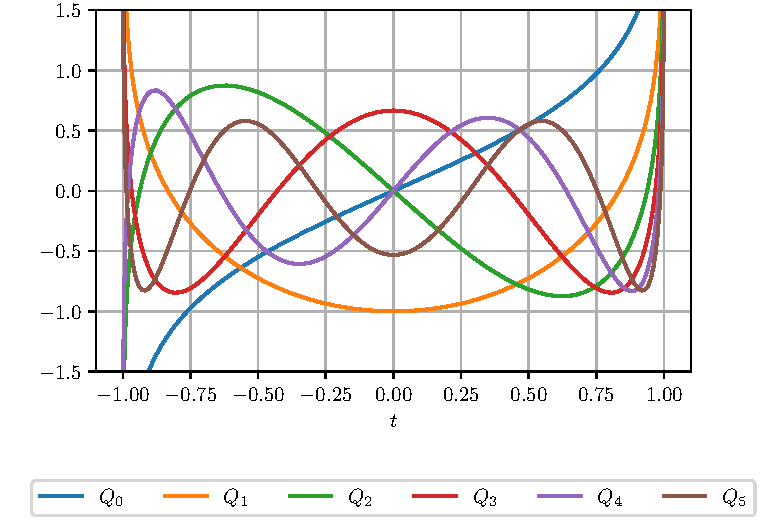
\includegraphics{./fig-legendre-polynomials-qn.pdf}
\caption{Legendreove polynómy~$Q_n(t)$ druhého druhu reálneho argumentu $t \in 
(-1, 1)$ pre~$n = 0, 1, \dots, 5$.  Z~dôvodu singularity nie sú Legendreove 
polynómy vypočítané pre~$t = -1$ a~$t = 1$.}
\label{fig:lp_2nd}
\end{figure}

\begin{figure}
\centering
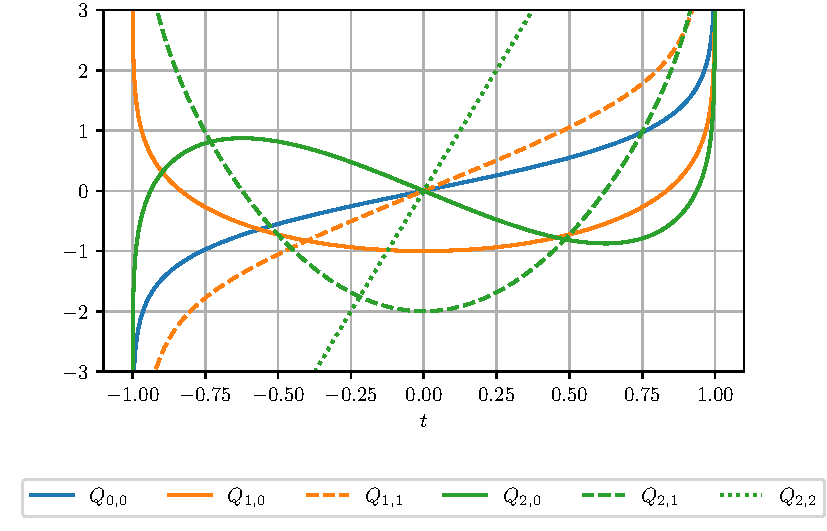
\includegraphics{./fig-legendre-functions-qnm.pdf}
\caption{Legendreove funkcie druhého druhu~$Q_{nm}(t)$ reálneho argumentu $t 
\in (-1, 1)$ pre~$n = 0, 1, 2$ a~$m = 0, \dots, n$.  Pre singularitu nie sú 
funkcie~$Q_{nm}(t)$ vypočítané v~koncových bodoch~$t = -1$ a~$t = 1$.}
\label{fig:lf_2nd}
\end{figure}

Rovnica~(\ref{eq:qnm_real_def}) je formálne podobná rovnici~(\ref{eq:pnm_def}).  
Napriek tomu, v~dôsledku rozdielnej definície derivovaných členov~$Q_n(t)$ ide 
o~funkcie s~odlišným priebehom ako~$P_{nm}(t)$.  Uveďme pre názornosť 
explicitné vzťahy na výpočet funkcií~$Q_0\left( t \right)$, $Q_1\left( 
t \right)$ a~$Q_2\left( t \right)$ reálneho argumentu~$t$ a~porovnajme ich 
s~rovnicami~(\ref{eq:p0_to_p5})
\parencite{MoritzPhysicalGeodesy},
%
\begin{align}
\label{eq:q0t}
Q_0(t) &= \frac{1}{2} \, \ln\frac{1 + t}{1 - t} = \mathrm{arctanh}(t){,}\\
%
\label{eq:q1t}
Q_1(t) &= \frac{t}{2} \, \ln\frac{1 + t}{1 - t} - 1 = t \, \mathrm{arctanh}(t)- 
 1{,}\\
%
\label{eq:q2t}
Q_2(t) &= \left( \frac{3}{4} t^2 - \frac{1}{4} \right) \, \ln\frac{1 + t}{1 
- t} - \frac{3}{2}t = \left( \frac{3}{2} t^2 - \frac{1}{2} \right) \, 
\mathrm{arctanh}(t) - \frac{3}{2}t{,}
\end{align}
%
kde
%
\begin{equation}
\label{eq:tanh}
\frac{1}{2} \, \ln \frac{1 + t}{1 - t} = \mathrm{arctanh} \, (t){.}
\end{equation}
%
Zápis $\mathrm{arctanh}$ označuje inverznú funkciu k~hyperbolickému 
tangensu~$\tanh$, ktorý je daný vzťahom \parencite{Gradshteyn2007}
%
\begin{equation}
\tanh t = \frac{e^t - e^{-t}}{e^t + e^{-t}}{.}
\end{equation}
%
Funkcie $Q_{nm}(t)$ pre niekoľko prvých stupňov~$n$ a~rádov~$m$ sú znázornené 
na Obrázkoch~\ref{fig:lp_2nd} a~\ref{fig:lf_2nd} (porovnaj 
s Obrázkami~\ref{fig:lp} a~\ref{fig:lf}).

Funkcie~$Q_0\left( z \right)$, $Q_1\left( z \right)$ a~$Q_2\left( z \right)$ 
komplexného argumentu~$z$ majú tvar
%
\begin{align}
\label{eq:q0z}
Q_0(z) &= \frac{1}{2} \, \ln\frac{z + 1}{z - 1} = \mathrm{arccoth}(z){,}\\
%
\label{eq:q1z}
Q_1(z) &= \frac{z}{2} \, \ln\frac{z + 1}{z - 1} - 1 = z \, \mathrm{arccoth}(z)- 
 1{,}\\
%
\label{eq:q2z}
Q_2(z) &= \left( \frac{3}{4} z^2 - \frac{1}{4} \right) \, \ln\frac{z + 1}{z 
- 1} - \frac{3}{2}z = \left( \frac{3}{2} z^2 - \frac{1}{2} \right) \, 
\mathrm{arccoth}(z) - \frac{3}{2}z{,}
\end{align}
%
pričom~$\mathrm{arccoth}$ je inverzná funkcia k hyperbolickému 
kotangensu~$\coth$ \parencite{Gradshteyn2007},
%
\begin{equation}
\coth z = \frac{1}{\tanh z} =  \frac{e^z + e^{-z}}{e^z - e^{-z}}{.}
\end{equation}

Pre~$Q_n(t)$ platia rovnaké rekurentné vzťahy ako pre~$P_n(t)$ 
\parencite{MoritzPhysicalGeodesy}.  Podobne ako funkcie $P_{nm}(t)$, i~funkcie 
$Q_{nm}(t)$ vyhovujú Legendreovej diferenciálnej rovnici druhého rádu 
\parencite[pozri rovnicu
\ref{eq:legfunc1_differential_equation};][]{MoritzPhysicalGeodesy}.  Všimnime 
si tiež, že pre $t \rightarrow \pm 1$, teda pre $\beta \rightarrow \pm 
\frac{\pi}{2}$, sa Legendreove funkcie druhého druhu blížia k~$\pm \infty$ 
(pozri rovnice~\ref{eq:qn0_imag_def} a~\ref{eq:qn0_real_def} 
a Obrázky~\ref{fig:lp_2nd} a~\ref{fig:lf_2nd}).  Túto vlastnosť budeme nazývať 
\emph{singularita}.  Práve kvôli singularite sa Legendreove funkcie druhého 
druhu nepoužívajú v~praktických aplikáciách ako riešenie pre funkcie 
$g_\mathrm{s}(\varphi)$ a~$g_\mathrm{r}(\beta)$ (rovnice~\ref{eq:gs} 
a~\ref{eq:gr}), a~to napriek tomu, že sú taktiež riešením Legendreovej 
diferenciálnej rovnice \parencite{MoritzPhysicalGeodesy}.

Presný a~efektívny numerický výpočet funkcií $Q_{nm}\left( i \frac{u}{E} 
\right)$ je náročný, obzvlášť pre vysoké stupne a~rády.  Z~dôvodov, ktoré budú 
ozrejmené neskôr v~Kapitole~\ref{sec:spheroidal_harmonic_expansion}, sa 
v~praktických geodetických aplikáciách nezvyknú počítať členy $Q_{nm}\left( 
i \frac{u}{E} \right)$, ale iba podiely $Q_{nm}\left( i \frac{u}{E} \right) 
\slash Q_{nm}\left( i \frac{b}{E} \right)$.  Samotný výpočet, či už funkcií 
$Q_{nm}\left( i \frac{u}{E} \right)$ alebo podielov $Q_{nm}\left( i \frac{u}{E} 
\right) \slash Q_{nm}\left( i \frac{b}{E} \right)$, je zvyčajne uskutočňovaný 
rekurentnými vzťahmi alebo rozvojmi do nekonečných radov \parencite[pozri 
napríklad][]{Sebera2012,Fukushima2013,Wang2013,Sprlak2020}.



\section{Rozvoj gravitačného potenciálu do radu sféroidických harmonických 
funkcií}
\label{sec:spheroidal_harmonic_expansion}

Gravitačný potenciál v~bodoch mimo telesa môže byť rozvinutý do radu 
sféroidických harmonických funkcií vzťahom \parencite{MoritzPhysicalGeodesy}
%
\begin{equation}
\label{eq:vg_spheroidalh_2nd_norm_ynk}
V_\gidx(u, \beta, \lambda) = \frac{GM}{R} \, \sum_{n = 0}^\infty \sum_{k 
= -n}^n \frac{Q_{n|k|}\left( i \dfrac{u}{E} \right)}{Q_{n|k|}\left( 
i \dfrac{b}{E} \right)} \, \bar{v}^{\mathrm{r}}_{nk} \, \bar{Y}_{nk}(\beta, 
\lambda){,}
\end{equation}
%
kde $\bar{v}_{nk}^\mathrm{r}$ sú \emph{úplne normované sféroidické harmonické 
koeficienty} gravitačného potenciálu.  
Rovnica~(\ref{eq:vg_spheroidalh_2nd_norm_ynk}) je lineárnou kombináciou funkcií 
(\ref{eq:fr}), (\ref{eq:gr}) a~(\ref{eq:hr}) (pozri tiež 
vzťah~\ref{eq:ynk_norm}), ktoré boli získané riešením Laplaceovej 
diferenciálnej rovnice v~redukovaných elipsoidických súradniciach metódou 
separácie premenných.  Rovnica~(\ref{eq:vg_spheroidalh_2nd_norm_ynk}) je 
formálne podobná vzťahu~(\ref{eq:vg_sh_2nd_norm_ynk}).  Môže byť tiež 
jednoducho prepísaná do tvaru, ktorý využíva index~$m = 0, 1, \dots, n$ 
(porovnaj rovnice~\ref{eq:vg_sh_2nd_norm} a~\ref{eq:vg_sh_2nd_norm_ynk}) či do 
radu nenormovaných sféroidických harmonických funkcií, podobne ako je tomu 
v~rovniciach~(\ref{eq:vg_sh_no_norm}) a~(\ref{eq:vg_sh_1st_norm}),
%
\begin{equation}
\label{eq:vg_spheroidalh_no_norm}
V_\gidx(u, \beta, \lambda) = \sum_{n = 0}^\infty \sum_{m = 0}^n 
\frac{Q_{nm}\left( i \dfrac{u}{E} \right)}{Q_{nm}\left( i \dfrac{b}{E} \right)} 
\, \left( C^{\mathrm{r}}_{nm} \, \cos(m\lambda) + S^{\mathrm{r}}_{nm} \, 
\sin(m\lambda) \right) \, P_{nm}(\sin\beta){.}
\end{equation}

Funkcia $Q_{n|k|}\left( i \frac{u}{E} \right)$ zo vzťahu~(\ref{eq:fr}) je 
komplexná funkcia.  Vo sféroidických harmonických 
rozvojoch~(\ref{eq:vg_spheroidalh_2nd_norm_ynk}) 
a~(\ref{eq:vg_spheroidalh_no_norm}) je preto vydelená funkciou $Q_{n|k|}\left( 
i \frac{b}{E} \right)$ tak, aby výsledný podiel bol reálne číslo.  Tým je 
zabezpečené, že i~sféroidické harmonické koeficienty sú reálne čísla.  Všimnime 
si tiež, že pred prvou sumáciou vo vzťahu~(\ref{eq:vg_spheroidalh_no_norm}) sa 
nenachádza Newtonova gravitačná konštanta~$G$ tak, ako je tomu vo 
vzťahu~(\ref{eq:vg_sh_no_norm}).  Ide len o~konvenciu, konštanta~$G$ je tým 
pádom obsiahnutá vo sféroidických harmonických 
koeficientoch~$C_{nm}^\mathrm{r}$~a~$S_{nm}^\mathrm{r}$.  
Rovnice~(\ref{eq:vg_spheroidalh_2nd_norm_ynk}) 
a~(\ref{eq:vg_spheroidalh_no_norm}) konvergujú vo vonkajšom priestore elipsoidu 
konvergencie (pozri Obrázok~\ref{fig:spheroidal_harmonics_convergence}).  Na 
povrchu elipsoidu konvergencie a/alebo v~jeho vnútri konvergencia zaručená nie 
je.

Podiel $Q_{n|k|}\left( i \frac{u}{E} \right) \slash Q_{n|k|}\left( 
i \frac{b}{E} \right)$ v~rovnici~(\ref{eq:vg_spheroidalh_2nd_norm_ynk}) má 
podobnú úlohu, akú má člen $\left( \frac{R}{r} \right)^{n + 1}$ 
vo~vzťahu~(\ref{eq:vg_sh_2nd_norm_ynk}), teda umožniť výpočet gravitačného 
potenciálu aj nad referenčným elipsoidom (v~prípade sférického harmonického 
rozvoja nad referenčnou sférou s~polomerom~$R$).  V~súvislosti 
s~rovnicou~(\ref{eq:ellred2cart}) sme uviedli, že pre~$E = 0$ sú redukované 
elipsoidické súradnice $u, \beta, \lambda$ totožné so sférickými súradnicami 
$r, \varphi, \lambda$.  Pre $E \rightarrow 0$ tiež platí vzťah 
\parencite{MoritzPhysicalGeodesy}
%
\begin{equation}
\lim_{E \rightarrow 0} \frac{Q_{n|k|}\left( i \dfrac{u}{E} 
\right)}{Q_{n|k|}\left( i \dfrac{b}{E} \right)} = \left( \frac{R}{r} \right)^{n 
+ 1}{.}
\end{equation}
%
Sférický harmonický rozvoj~(\ref{eq:vg_sh_2nd_norm_ynk}) preto možno považovať 
za špeciálny prípad zovšeobecneného sféroidického harmonického 
rozvoja~(\ref{eq:vg_spheroidalh_2nd_norm_ynk}).

Na záver dodajme, že Laplaceovu rovnicu možno riešiť aj v~súradnicovom systéme, 
ktorý je vztiahnutý k~trojosovému elipsoidu s~polosami $a$, $b$, $c$.  Získame 
tým rozvoj gravitačného potenciálu do radu elipsoidických harmonických funkcií 
\parencite[napríklad][]{Garmier2001,Hu2015,Reimond2016}.  Tento prístup je 
zložitejší ako sférické a~sféroidické harmonické rozvoje a~vo fyzikálnej 
geodézii sa využíva zriedkavo.  Uplatnenie má najmä v~modelovaní gravitačného 
poľa v~blízkosti asteroidov, ktoré majú komplikovaný tvar.








% -----------------------------------------------------------------------------


\chapter{Normálne tiažové pole}
\label{sec:normal_gravity_field}

Tvar Zeme v~podobe \emph{geometrickej} výšky nad zvolenou referenčnou plochou 
možno určiť geometrickými metódami, napríklad fotogrametriou, družicovou 
radarovou interferometriou či leteckým laserovým skenovaním \parencite[pozri 
napríklad][]{Hirt2014c}.  Na určenie \emph{fyzikálnych} výšok je potrebné 
uvážiť nielen geometrickú, ale aj fyzikálnu časť výšky 
(Kapitola~\ref{sec:heights}).  Fyzikálna geodézia preto určuje tvar Zeme 
z~informácie o~jej tiažovom poli, napríklad z~tiažového potenciálu 
a~z~tiažového zrýchlenia na povrchu Zeme.

Určenie tvaru Zeme z~jej tiažového poľa je neľahké, pretože vzťah medzi 
tiažovým poľom a~hľadaným zemským povrchom je nelineárny.  Spravidla sa preto 
pristupuje k~linearizácii pomocou rozvoja do Taylorovho radu, pričom členy 
druhého a~vyšších rádov sa zanedbajú.  \emph{Normálne tiažové pole Zeme} je 
jednoduchý a~súčasne dostatočne presný model skutočného tiažového poľa Zeme 
a~slúži práve na výpočet približných hodnôt v~linearizovaných úlohách 
fyzikálnej geodézie.  Požiadavka jednoduchosti je odôvodnená potrebou 
prijateľne náročných výpočtov v~normálnom poli, napríklad pomocou uzavretých 
vzťahov pre \emph{normálne tiažové zrýchlenie} $\boldsymbol{\gamma}$ či 
\emph{normálny tiažový potenciál} $U$.  Dostatočná presnosť je potrebná nato, 
aby nelineárne členy Taylorovho rozvoja mohli byť s~rozumnou mierou aproximácie 
zanedbané.  Požiadavky jednoduchosti a~presnosti si vzájomne odporujú, preto je 
potrebné nájsť medzi nimi vhodný kompromis.

Povedané inak, normálne tiažové pole Zeme umožňuje redukciu veličín skutočného 
tiažového poľa Zeme o~približné hodnoty (napríklad skutočné tiažové 
zrýchlenie~$\vec g$ zredukujeme o~normálne tiažové 
zrýchlenie~$\boldsymbol{\gamma}$).  Získame tým rozličné reziduálne veličiny, 
ktoré majú praktické využitie nielen v~geodézii, ale aj v~mnohých iných 
geovedných disciplínach.  Príkladom je geofyzika, ktorá využíva normálne 
tiažové pole Zeme okrem iného na štúdium hustotných kontrastov pod zemským 
povrchom.  Veličiny, ktoré získame po redukcii skutočného tiažového poľa 
o~normálne tiažové pole, budú popísané 
v~Kapitole~\ref{sec:disturbing_field_deflections}.  V~tejto kapitole 
predstavíme koncept normálneho poľa.

\section{Voľba normálneho tiažového poľa}
\label{sec:choice_of_normal_gravity_field}

\subsection{Homogénna rotujúca guľa}
\label{sec:normal_field_ball}

Homogénna rotujúca guľa (Kapitola~\ref{sec:homogeneous_ball}) je jedno 
z~najjednoduchších telies, ktoré by mohlo generovať normálne tiažové pole Zeme.  
Táto voľba je však nevhodná z~dvoch dôvodov.  Prvým je sférický tvar gule, 
ktorý nereprezentuje dostatočne presne sploštený tvar Zeme.  Druhý dôvod je 
ten, že tiažový potenciál na povrchu homogénnej rotujúcej gule nie je 
konštantný (Kapitola~\ref{sec:homogeneous_ball_gravity_field}).  Homogénna guľa 
je tu považovaná za tuhé teleso, ktoré v~dôsledku vlastnej gravitácie 
a~odstredivej sily nemení svoj tvar \parencite{SansoGeoidDetermination}.  Zem 
ale nie je tuhé teleso (Kapitola~\ref{sec:time_variable_gravity}), a~tak pod 
vplyvom spomenutých síl mení svoj tvar, pričom sa snaží ustáliť v~rovnovážnej 
polohe.  Zmena tvaru zemského telesa v~dôsledku vlastnej gravitácie 
a~odstredivej sily je jednoducho predstaviteľná pre~tekutú časť zemského 
povrchu.  Tá má tendenciu ustáliť sa v~rovnovážnej polohe, ktorou je plocha 
s~konštantnou hodnotou skutočného tiažového potenciálu, teda geoid.  Je preto 
vhodné požadovať od normálneho tiažového poľa, aby jeho referenčná plocha, 
ktorá aproximuje geoid nielen geometricky, ale aj fyzikálne, bola súčasne aj 
ekvipotenciálnou plochou.

Dodajme ale, že v~niektorých úlohách fyzikálnej geodézie je vplyv normálneho 
tiažového poľa dostatočné malý na to, aby bolo možné použiť \emph{gravitačné} 
pole \emph{nerotujúcej} homogénnej gule \parencite{SansoGeoidDetermination}, 
ktorá má na svojom povrchu konštantný \emph{gravitačný} potenciál 
(Kapitola~\ref{sec:homogeneous_ball_gravitational_field}).

\subsection{Ekvipotenciálny elipsoid}
\label{sec:normal_field_equipotential_ellipsoid}

\emph{Ekvipotenciálny elipsoid} je dvojosový rotačný elipsoid, ktorý má na 
svojom povrchu konštantný normálny tiažový potenciál.  V~súčasnosti je 
najčastejšou voľbou pre definíciu normálneho tiažového poľa Zeme.

Ekvipotenciálny elipsoid je vhodným praktickým riešením oboch problémov, ktoré 
sú spojené s~normálnym tiažovým poľom homogénnej rotujúcej gule.  V~prvom rade, 
dvojosový rotačný elipsoid je vernejšou geometrickou aproximáciou sploštenej 
Zeme ako sféra, čím ponúka uspokojivejšie riešenie problému tvaru referenčnej 
plochy.  Druhá požiadavka spojená s~konštantnou hodnotou normálneho tiažového 
potenciálu na referenčnej ploche bola vyriešená jednoducho tým, že referenčný 
elipsoid sme vyhlásili za ekvipotenciálny.  Nepotrebovali sme pritom vysloviť 
žiadny predpoklad o~priestorovom rozložení hustôt v~ekvipotenciálnom elipsoide.  
Je to preto, lebo fyzikálna geodézia sa zaoberá určovaním tvaru 
a~\emph{vonkajšieho} tiažového poľa Zeme a~normálne tiažové pole využíva 
predovšetkým na účely linearizácie.  Zdá sa byť preto kľúčové najmä to, aby 
normálna ekvipotenciálna plocha s~normálnym tiažovým potenciálom~$U_0$ bola 
geometricky blízka geoidu, ďalej aby normálny tiažový potenciál~$U_0$ bol 
blízky skutočnému tiažovému potenciálu~$W_0$ na geoide, a~nakoniec aby 
geometrická aj fyzikálna časť normálneho poľa boli jednoducho matematicky 
opísateľné.  Vhodne definovaný ekvipotenciálny elipsoid spĺňa všetky tieto 
požiadavky.  Pre niektoré príbuzné vedné odbory, napríklad pre geofyziku, je 
však znalosť hustoty v~normálnom telese potrebná \parencite{Karcol2017}.  
V~takýchto situáciách nemusí byť voľba ekvipotenciálneho elipsoidu tá 
najvýhodnejšia.  Diskusiu k~možnostiam priestorového rozloženia hustoty vo 
vnútri ekvipotenciálneho elipsoidu je možné nájsť napríklad v~prácach 
\textcite{MoritzTheFigureOfTheEarth}, \textcite{Conway2000}, 
\textcite{TorgeGeodesy} a~\textcite{Karcol2017}.

Inými slovami, tak ako homogénna rotujúca guľa, ani ekvipotenciálny elipsoid 
nie je ideálne riešenie, ktoré by bolo fyzikálne odôvodniteľné.  Z~hľadiska 
fyzikálnej geodézie je ale jeho veľkou prednosťou skutočnosť, že ponúka 
dostatočne dobré praktické riešenie pre v~zásade všetky súčasné problémy, ktoré 
sú spojené s~linearizovanými úlohami určovania tvaru Zeme a~jej vonkajšieho 
tiažového poľa.  V~konečnom dôsledku, aj Newtonov gravitačný zákon je nesprávny 
a~je iba priblížením skutočnosti (pozri úvodnú kapitolu).  Napriek tomu ho ale 
používame, pretože umožňuje riešiť mnohé úlohy fyzikálnej geodézie dostatočne 
presne a~relatívne jednoducho.

Ekvipotenciálny elipsoid má navyše ďalšiu silnú stránku.  Pre mnohé úlohy 
geodézie (napríklad určovanie polohy GNSS metódami) môže vďaka svojmu 
sploštenému tvaru súčasne plniť aj úlohu geometrického referenčného systému.  
Tým sú opäť prepojené geometrická a~fyzikálna zložka geodézie, ktoré sú 
potrebné pre určovanie polohy aj pre určovanie tiažového poľa (pozri 
Kapitolu~\ref{sec:equipotential_surface}).

\subsection{Sféroid}
\label{sec:normal_field_spheroid}

Ďalšou možnosťou voľby normálneho tiažového poľa je sférický harmonický rozvoj 
gravitačného potenciálu do vopred zvoleného konečného harmonického stupňa 
(rovnice~\ref{eq:vg_sh_no_norm}, \ref{eq:vg_sh_1st_norm}, 
\ref{eq:vg_sh_2nd_norm} a~\ref{eq:vg_sh_2nd_norm_ynk}).  Plocha, na ktorej je 
takto definovaný normálny tiažový potenciál konštantný, sa nazýva 
\emph{sféroid}.\footnote{V~Kapitole~\ref{sec:spheroidal_harmonics_chapter} sme 
za sféroid považovali dvojosový elipsoid.  Ten je špeciálnym prípadom 
všeobecnejšie chápaného pojmu \emph{sféroid} z~tejto kapitoly.}  Obmedzením 
rozvoja potenciálu na stupeň~2 získame \emph{Brunsov sféroid} a~obmedzením na 
stupeň~4 získame \emph{Helmertov sféroid} \parencite{Moritz1967}.  Oba sféroidy 
majú koeficienty stupňa~1 nulové, pretože začiatok súradnicového systému je 
vložený do geometrického stredu ekvipotenciálneho elipsoidu 
(pozri~Kapitolu~\ref{sec:physical_meaning_of_spherical_harmonic_coefficients}).  
Helmertov sféroid má nulové navyše aj koeficienty stupňa~3, aby bola 
zabezpečená symetria normálneho poľa voči rovine rovníka (pozri geometrickú 
interpretáciu sférických harmonických funkcií 
v~Kapitole~\ref{sec:spherical_harmonics}).   V~súčasnosti sa Brunsov ani 
Helmertov sféroid nezvyknú používať.  Obe plochy sú totiž veľmi blízke 
dvojosovému rotačnému elipsoidu a~dodatočná presnosť je získaná za cenu výrazne 
náročnejšieho matematického popisu oboch plôch.  To odporuje požiadavke 
jednoduchosti z~Kapitoly~\ref{sec:normal_gravity_field}.  Navyše, dodatočná 
presnosť, ktorú získame použitím Brunsovho alebo Helmertovho sféroidu, zväčša 
nie je významná \parencite{Moritz1967}.



\section{Ekvipotenciálny elipsoid}
\label{sec:equipotential_ellipsoid}

Nech teleso s~hmotnosťou~$M$ rotuje okolo pevnej osi konštantnou uhlovou 
rýchlosťou rotácie~$\omega$.  Nech $S$ je ekvipotenciálna plocha jeho tiažového 
poľa, ktorá obklopuje celé teleso.  \emph{Stokesov--Poincarého} teorém hovorí, 
že tiažový potenciál vo vonkajšom priestore plochy~$S$ je jednoznačne určený 
konštantami $M$ a~$\omega$ a~parametrami, ktoré definujú plochu~$S$ 
\parencite{TorgeGeodesy}.  G.~G.~Stokes (1819~-- 1903) bol írsko--anglický 
matematik a fyzik, ktorý významne prispel do viacerých vedných odvetví, 
napríklad do mechaniky tekutín (Navierova--Stokesova rovnica) či do optiky 
(polarizácia svetla).  H.~Poincaré (1854~-- 1912) bol francúzsky matematik 
a~teoretický fyzik.  V~geodézii je známy napríklad pre redukciu tiažového 
zrýchlenia z~povrchu Zeme dovnútra Zeme (pozri 
Kapitolu~\ref{sec:helmert_height}).

Na jednoznačné definovanie ekvipotenciálneho elipsoidu a~jeho vonkajšieho 
tiažového poľa teda postačuje definovať štyri nezávislé \emph{základné 
parametre}.  Dva z~týchto parametrov sú geometrické, resp. veľmi úzko súvisia 
s~geometriou elipsoidu (napríklad hlavná polos a~sploštenie elipsoidu), a~dva 
parametre sú fyzikálne (hmotnosť a~uhlová rýchlosť rotácie).  Zo základných 
parametrov je možné vypočítať všetky ostatné veličiny normálneho tiažového 
poľa, či už ide o~geometrické parametre (napríklad vedľajšia polos či lineárna 
excentricita elipsoidu) alebo o~fyzikálne parametre (normálny tiažový 
potenciál, normálne tiažové zrýchlenie a pod.).  Parametre, ktoré sú vypočítané 
zo základných parametrov, budeme nazývať \emph{odvodené parametre}.  Teóriu 
ekvipotenciálneho elipsoidu rozpracovali taliansky geodet, astronóm, geofyzik 
a~matematik P.~Pizzetti (1860--1918) a~taliansky matematik a~matematický fyzik 
C.~Somigliana (1860--1955) v~prácach \textcite{Pizzetti1984} 
a~\textcite{Somigliana1929}.

Základné parametre ekvipotenciálnych elipsoidov sú v~súčasnosti určované 
spravidla družicovými technikami a~astronomickými meraniami.  Historický 
prehľad geodetických referenčných systémov a~spôsobov ich určenia je dostupný 
napríklad v~prácach \textcite{TorgeGeodesy} a~\textcite{MoritzPhysicalGeodesy}.  
Na nasledujúcich stranách popíšeme dva najpoužívanejšie ekvipotenciálne 
elipsoidy (Kapitoly~\ref{sec:grs80} a~\ref{sec:wgs84}).  Následne odvodíme 
vzťahy na výpočet normálneho tiažového potenciálu pomocou rozvoja do radu 
sféroidických a~sférických harmonických 
funkcií~(Kapitola~\ref{sec:normal_gravity_potential}).  Na záver opíšeme spôsob 
výpočtu normálneho tiažového zrýchlenia (Kapitola~\ref{sec:normal_gravity}).  
Tieto poznatky budú dôležité neskôr v~Kapitole~\ref{sec:geoid}, ktorá sa 
zaoberá určovaním geoidu.  Po celý čas je pritom vhodné mať na pamäti, že 
normálne tiažové pole Zeme je matematicko-fyzikálny model, ktorý je definovaný 
niekoľkými základnými parametrami.  Všetky ostatné parametre, či už geometrické 
alebo fyzikálne, sú odvodené zo základných parametrov.  S~výnimkou základných 
parametrov sa teda všetky veličiny normálneho tiažového poľa získavajú 
výpočtom, nie meraním ako je tomu v~prípade \emph{skutočného} tiažového poľa 
Zeme.





\subsection{Ekvipotenciálny elipsoid GRS80}
\label{sec:grs80}

Jednu z~možných štvoríc základných parametrov ekvipotenciálneho elipsoidu tvorí
%
\begin{itemize}
\item hlavná polos~$a$,
%
\item dynamický koeficient~$J_{2,0}$,
%
\item geocentrická gravitačná konštanta~$GM$~a
%
\item uhlová rýchlosť rotácie $\omega$.
\end{itemize}
%
Týmito základnými parametrami je definovaný ekvipotenciálny elipsoid 
\emph{GRS80} \parencite[angl. \textit{Geodetic Reference 
System~1980};][]{GRS80}.  Základné parametre GRS80 
(Tabuľka~\ref{tab:grs80_fundamental}) boli prijaté Medzinárodnou úniou geodézie 
a geofyziky (angl.~\textit{International Union of Geodesy and Geophysics}, 
IUGG) a~Medzinárodnou asociáciou geodézie IAG na 17.~generálnom zasadnutí IUGG 
v Canberra v~decembri 1979.

\begin{table*}
\begin{center}
\caption{Základné parametre ekvipotenciálneho elipsoidu GRS80 
\parencite{GRS80}.}
\label{tab:grs80_fundamental}
\small
\begin{tabular}{l l l l}
\hline
Označenie & Hodnota & Jednotka & Popis\\
\hline
$a$       & $6\,378\,137$ & m & Hlavná polos\\
$J_{2,0}$ & $108\,263 \times 10^{-8}$ & Bezrozmerné & Dynamický faktor\\
$GM$ & $3\,986\,005 \times 10^8$ & $\mathrm{m}^3 \ \mathrm{s}^{-2}$ 
& Geocentrická gravitačná konštanta\\
$\omega$ & $7\,292\,115 \times 10^{-11}$ & $\mathrm{rad} \ \mathrm{s}^{-1}$ 
& Uhlová rýchlosť rotácie\\
\hline
\end{tabular}
\end{center}
\end{table*}

Všimnime si, že medzi základnými parametrami sa nachádza geocentrická 
gravitačná konštanta $GM$ a~nie hmotnosť Zeme~$M$, ktorá je podľa 
Stokesovho--Poincarého teorému postačujúca na jednoznačné definovanie tiažového 
potenciálu vo vonkajšom priestore ekvipotenciálneho elipsoidu 
(Kapitola~\ref{sec:equipotential_ellipsoid}).  Dôvod je ten, že konštantu~$GM$ 
dokážeme určiť presnejšie ako konštantu~$M$ (pozri 
Kapitolu~\ref{sec:homogeneous_ball_gravitational_field}).  Spomeňme tiež, že 
hodnota konštanty~$GM$ z~Tabuľky~\ref{tab:grs80_fundamental} zahŕňa hmotnosť 
Zeme aj hmotnosť zemskej atmosféry a~koeficient~$J_{2,0}$ nezahŕňa účinok 
permanentnej slapovej deformácie Zeme.  Medzi koeficientmi~$J_{2,0}$ 
(Tabuľka~\ref{tab:grs80_fundamental}), $C_{2,0}$ 
(rovnica~\ref{eq:vg_sh_no_norm}) a~$\bar{C}_{2,0}$ 
(rovnica~\ref{eq:vg_sh_2nd_norm}) platia nasledovné vzťahy 
\parencite{Moritz1967,MoritzPhysicalGeodesy},
%
\begin{align}
\label{eq:c20_j20}
C_{2,0} &= -J_{2,0}{,}\\
%
\label{eq:c20_j20_2}
\bar{C}_{2,0} &= \frac{C_{2,0}}{\sqrt{5}} = -\frac{J_{2,0}}{\sqrt{5}}{.}
\end{align}

Tabuľka~\ref{tab:grs80_derived} uvádza číselné hodnoty niektorých odvodených 
geometrických a fyzikálnych parametrov ekvipotenciálneho elipsoidu~GRS80.  
Medzi geometrické parametre sme zahrnuli, okrem iných, prvú numerickú 
excentricitu (vzťah~\ref{eq:1st_eccentricity}), \emph{druhú numerickú 
excentricitu}
%
\begin{equation}
\label{eq:2nd_eccentricity}
e' = \frac{\sqrt{a^2 - b^2}}{b}{,}
\end{equation}
%
a \emph{sploštenie}
%
\begin{equation}
\label{eq:flattening}
f = \frac{a - b}{a}{.}
\end{equation}
%
Vzťahy na výpočet odvodených fyzikálnych parametrov 
z~Tabuľky~\ref{tab:grs80_derived} budú uvedené neskôr.

\begin{table*}
\begin{center}
\caption{Niektoré odvodené parametre ekvipotenciálneho elipsoidu GRS80 
\parencite{MoritzPhysicalGeodesy}.}
\label{tab:grs80_derived}
\small
\begin{tabular}{l l l l l}
\hline
Typ parametra & Symbol & Hodnota & Jednotka & Popis\\
\hline
Geometrický & $b$       & $6 \, 356 \, 752.3141$ & m & Vedľajšia polos\\
            & $E$       & $521 \, 854.0097$ & m & Lineárna excentricita\\
            & $e^2$     & $0.00669438002290$ & Bezrozmerné & Druhá mocnina 
            prvej\\
            &           &     &             & numerickej excentricity\\
            & $(e')^2$  & $0.00673949677548$ & Bezrozmerné & Druhá mocnina 
            druhej\\
            &           &     &             & numerickej excentricity\\
            & $f$       & $0.00335281068118$ & Bezrozmerné & Sploštenie\\
\hline
Fyzikálny & $U_0$       & $ 62 \, 636 \, 860.850$ & $\mathrm{m}^2 \, 
          \mathrm{s}^{-2}$ & Normálny tiažový\\
          &            &     &   & potenciál na elipsoide\\
          & $\gamma_a$ & $9.7803267715$ & $\mathrm{m} \, \mathrm{s}^{-2}$ 
& Normálne tiažové\\
          &            &     &   & zrýchlenie na rovníku\\
          & $\gamma_b$ & $9.8321863685$ & $\mathrm{m} \, \mathrm{s}^{-2}$ 
& Normálne tiažové\\
          &            &     &   & zrýchlenie na póle\\
          & $m$ & $0.00344978600308$ & Bezrozmerné & Pomocná konštanta,\\
          &     &                    &             & $m = \omega^2 \, a^2 \, 
b \slash (GM)$\\
\hline
\end{tabular}
\end{center}
\end{table*}

Elipsoid GRS80 je oficiálny referenčný systém Medzinárodnej asociácie geodézie.






\subsection{Ekvipotenciálny elipsoid WGS84}
\label{sec:wgs84}

\begin{table*}
\begin{center}
\caption{Základné parametre ekvipotenciálneho elipsoidu WGS84 
\parencite{WGS84}.}
\label{tab:wgs84_fundamental}
\small
\begin{tabular}{l l l l}
\hline
Označenie & Hodnota & Jednotka & Popis\\
\hline
$a$       & $6\,378\,137$ & m & Hlavná polos\\
$1 \slash f$ & $298.257223563$ & Bezrozmerné & Prevrátená hodnota sploštenia\\
$GM$ & $3\,986\,004.418 \times 10^8$ & $\mathrm{m}^3 \ \mathrm{s}^{-2}$ 
& Geocentrická gravitačná konštanta\\
$\omega$ & $7\,292\,115 \times 10^{-11}$ & $\mathrm{rad} \ \mathrm{s}^{-1}$ 
& Uhlová rýchlosť rotácie\\
\hline
\end{tabular}
\end{center}
\end{table*}

Ďalšou možnosťou definície ekvipotenciálneho elipsoidu je použiť sploštenie~$f$ 
(rovnica~\ref{eq:flattening}) namiesto koeficientu~$J_{2,0}$.  Týmto spôsobom 
je definovaný ekvipotenciálny elipsoid \emph{WGS4} 
\parencite[angl. \textit{World Geodetic System~1984};][]{WGS84}, ktorý vychádza 
z~elipsoidu GRS80 (Tabuľka~\ref{tab:wgs84_fundamental}).  Vybraté odvodené 
parametre elipsoidu WGS84 sú uvedené v~Tabuľke~\ref{tab:wgs84_derived}.  
Z hľadiska tvaru sú oba elipsoidy podobné; dĺžka ich hlavnej polosi je $6\, 
378\, 137\ \mathrm{m}$ a~dĺžka vedľajšej polosi, vypočítaná zo základných 
parametrov, sa odlišuje iba o~desatinu milimetra (porovnaj 
Tabuľky~\ref{tab:grs80_derived} a~\ref{tab:wgs84_derived}).  Z~fyzikálneho 
hľadiska je už medzi elipsoidmi väčší rozdiel.  Uhlová rýchlosť rotácie oboch 
elipsoidov je síce rovnaká, no odlišné hodnoty geocentrických gravitačných 
konštánt spôsobujú rozdielny normálny tiažový potenciál na elipsoide.  Rozdiel 
medzi hodnotami normálneho tiažového potenciálu na elipsoide je približne o~5 
rádov väčší ako v~súčasnosti dosiahnuteľná presnosť určenia rozdielu skutočného 
tiažového potenciálu medzi dvoma bodmi, ktoré sú od seba vzdialené niekoľko 
kilometrov (pozri Kapitolu~\ref{sec:potential_differences}).

\begin{table*}
\begin{center}
\caption{Niektoré odvodené parametre ekvipotenciálneho elipsoidu WGS84 
\parencite{MoritzPhysicalGeodesy}.}
\label{tab:wgs84_derived}
\small
\begin{tabular}{l l l l l}
\hline
Typ parametra & Symbol & Hodnota & Jednotka & Popis\\
\hline
Geometrický & $b$       & $6 \, 356 \, 752.3142$ & m & Vedľajšia polos\\
            & $E$       & $521 \, 854.0084$ & m & Lineárna excentricita\\
            & $e^2$     & $0.00669437999014$ & Bezrozmerné & Druhá mocnina 
            prvej\\
            &           &     &             & numerickej excentricity\\
            & $(e')^2$  & $0.00673949674228$ & Bezrozmerné & Druhá mocnina 
            druhej\\
            &           &     &             & numerickej excentricity\\
            & $J_{2,0}$       & $108262.982131 \times 10^{-8}$ & Bezrozmerné 
& Dynamický faktor\\
\hline
Fyzikálny & $U_0$       & $ 62 \, 636 \, 851.715$ & $\mathrm{m}^2 \, 
          \mathrm{s}^{-2}$ & Normálny tiažový\\
          &            &     &   & potenciál na elipsoide\\
          & $\gamma_a$ & $9.7803253359$ & $\mathrm{m} \, \mathrm{s}^{-2}$ 
& Normálne tiažové\\
          &            &     &   & zrýchlenie na rovníku\\
          & $\gamma_b$ & $9.8321849378$ & $\mathrm{m} \, \mathrm{s}^{-2}$ 
& Normálne tiažové\\
          &            &     &   & zrýchlenie na póle\\
          & $m$ & $0.00344978650684$ & Bezrozmerné & Pomocná konštanta,\\
          &     &                    &             & $m = \omega^2 \, a^2 \, 
b \slash (GM)$\\
\hline
\end{tabular}
\end{center}
\end{table*}






\section{Normálny tiažový potenciál}
\label{sec:normal_gravity_potential}

V~mnohých situáciách, hoci rozhodne nie v~každej situácii, sú 
preferované~uzavreté matematické vzťahy pred nekonečnými rozvojmi.  Uzavretý 
vzťah je taký vzťah, ktorý má konečný počet členov.  Často umožňuje presnejší 
a rýchlejší číselný výpočet v~porovnaní s~jeho nekonečným náprotivkom, pretože 
ten musí byť vždy obmedzený na vhodne zvolený konečný počet členov.  
V~Kapitole~\ref{sec:normal_gravity_potential_in_reduced_ell_coords} budeme 
preto hľadať uzavretý vzťah na výpočet normálneho tiažového potenciálu~$U$ 
v~bodoch na povrchu ekvipotenciálneho elipsoidu a~nad ním.  Pracovať budeme 
v~redukovaných elipsoidických súradniciach, ktoré sa prirodzene ponúkajú 
v~súvislosti so splošteným rotačným elipsoidom.  Následne 
v~Kapitole~\ref{sec:normal_gravity_potential_in_spherical_coords} vyjadríme 
normálny tiažový potenciál vo sférických súradniciach, tentokrát už ale pomocou 
nekonečného rozvoja.  
Kapitola~\ref{sec:normal_gravity_potential_in_reduced_ell_coords} je spracovaná 
podľa~\textcite{MoritzTheFigureOfTheEarth}.



\subsection{Normálny tiažový potenciál v~redukovaných elipsoidických 
súradniciach}
\label{sec:normal_gravity_potential_in_reduced_ell_coords}

Vzťah~(\ref{eq:vg_spheroidalh_no_norm}) popisuje vonkajší gravitačný potenciál 
všeobecného telesa.  Ak k nemu pripočítame odstredivý potenciál, získame vzťah 
pre tiažový potenciál $W$ všeobecného telesa (pozri rovnicu~\ref{eq:w}).  
Normálny tiažový potenciál~$U$ ekvipotenciálneho elipsoidu je ale opísateľný 
jednoduchším spôsobom ako tiažový potenciál všeobecného telesa.  Dôvodom sú dve 
symetrie normálneho poľa, jedna voči osi rotácie a~druhá voči rovine rovníka.  
Prvá symetria spôsobuje, že všetky nezonálne sféroidické harmonické 
funkcie~v~rovnici~(\ref{eq:vg_spheroidalh_no_norm}) musia byť nulové, pretože 
závisia od dĺžky~$\lambda$.  Vďaka druhej symetrii sú nenulové iba párne 
zonálne sféroidické harmonické funkcie (pozri vlastnosti sférických 
harmonických funkcií v~Kapitole~\ref{sec:spherical_harmonics}).  Normálny 
tiažový potenciál ekvipotenciálneho elipsoidu teda môžeme zapísať v~tvare
%
\begin{equation}
\label{eq:u_sph}
U(u, \beta) = U_\gidx(u, \beta) + U_\cidx(u, \beta){,}
\end{equation}
%
pričom normálny gravitačný potenciál~$U_\gidx(u, \beta)$ je daný vzťahom (pozri 
rovnicu~\ref{eq:vg_spheroidalh_no_norm})
%
\begin{equation}
\label{eq:ug_sph}
U_\gidx(u, \beta) = \sum_{n = 0}^\infty \frac{Q_n\left( i \dfrac{u}{E} 
\right)}{Q_n\left( i \dfrac{b}{E} \right)} \,  C^{\mathrm{r}}_n \, 
P_n(\sin\beta)
\end{equation}
%
a~normálny odstredivý potenciál~$U_\cidx(u, \beta)$ je daný vzťahom (pozri 
rovnice~\ref{eq:vc} a~\ref{eq:ellred2cart})
%
\begin{equation}
\label{eq:uc_sph}
U_\cidx(u, \beta) = \frac{1}{2} \, \omega^2 \, (u^2 + E^2) \, \cos^2\beta{.}
\end{equation}
%
Pre lepšiu názornosť nasledujúcich krokov sme do vzťahu~(\ref{eq:ug_sph}) 
zahrnuli aj nepárne zonálne koeficienty~$C^{\mathrm{r}}_n$ hoci sú nulové.  
Dodajme, že normálny gravitačný potenciál vyhovuje Laplaceovej rovnici vo 
vonkajšom priestore elipsoidu,
%
\begin{equation}
\label{eq:ug_laplace_cart}
\nabla^2 U_\gidx = \frac{\partial^2 U_\gidx}{\partial x^2} + \frac{\partial^2 
U_\gidx}{\partial y^2} + \frac{\partial^2 U_\gidx}{\partial z^2} = 0{.}
\end{equation}

Z Kapitoly~\ref{sec:spherical_harmonic_expansion} vieme, že ak chceme poznať 
$U(u,\beta)$ z~rovnice~(\ref{eq:u_sph}), potom potrebujeme poznať 
koeficienty~$C_n^\mathrm{r}$.  Zatiaľ čo v~prípade skutočného poľa Zeme je 
potrebné koeficienty~$C_{nm}$ a~$S_{nm}$ (rovnica~\ref{eq:vg_sh_no_norm}) 
vypočítať z~meraní skutočného poľa 
(Kapitola~\ref{sec:sh_applications_gravity_field}), koeficienty normálneho poľa 
$C_n^\mathrm{r}$ je možné vypočítať zo základných parametrov ekvipotenciálneho 
elipsoidu.  Hľadajme preto vzťah medzi sféroidickými harmonickými koeficientmi 
$C_n^\mathrm{r}$ a~základnými parametrami ekvipotenciálneho elipsoidu.

Nech sa výpočtový bod nachádza na povrchu ekvipotenciálneho elipsoidu, teda $u 
= b$.  Potom
%
\begin{equation}
\frac{Q_n\left( i \dfrac{u}{E} \right)}{Q_n\left( i \dfrac{b}{E} \right)} 
= 1{,} \quad u = b{,}
\end{equation}
%
a rovnica~(\ref{eq:u_sph}) prejde do tvaru
%
\begin{equation}
\label{eq:u_sph_on_ell}
U(b, \beta) = \sum_{n = 0}^\infty C^{\mathrm{r}}_n \, P_n(\sin\beta) 
+ \frac{1}{2} \, \omega^2 \, (b^2 + E^2) \, \cos^2\beta = U_0{.}
\end{equation}

Rovnica~(\ref{eq:u_sph_on_ell}) je formálne podobná 
vzťahu~(\ref{eq:f_synthesis}) avšak s~dvoma rozdielmi.  Po prvé, na ľavej 
strane rovnice nie je funkcia $f(t)$, ktorá by závisela od $t = \sin\beta$, ale 
konštanta $U(b, \beta) = U_0$ (normálny tiažový potenciál na ekvipotenciálnom 
elipsoide je z~definície konštantný, pozri 
Kapitolu~\ref{sec:equipotential_ellipsoid}).  Po druhé, prostredná časť rovnice 
obsahuje člen~$\cos^2\beta$, ktorý, podobne ako Legendreove 
polynómy~$P_n(\sin\beta)$, závisí od $\sin\beta$, pretože $\cos^2\beta 
= 1 - \sin^2\beta$.  Pomocou vzťahov (rovnica~\ref{eq:linear_eccentricity})
%
\begin{equation}
a^2 = b^2 + E^2
\end{equation}
%
a (rovnica~\ref{eq:p0_to_p5})
%
\begin{equation}
P_2(\sin\beta) = \frac{3}{2} \, \sin^2\beta - \frac{1}{2}
\end{equation}
%
preto prepíšme rovnicu~(\ref{eq:u_sph_on_ell}) do tvaru
%
\begin{equation}
\label{eq:cnr}
\sum_{n = 0}^\infty C^{\mathrm{r}}_n \, P_n(\sin\beta) + \frac{1}{3} \, 
\omega^2 \, a^2  - \frac{1}{3} \, \omega^2 \, a^2 \, P_2(\sin\beta) - U_0 
= 0{.}
\end{equation}

Keďže $P_0(\sin\beta) = 1$ (rovnica~\ref{eq:p0_to_p5}), vzťah~(\ref{eq:cnr}) 
môžeme ďalej upraviť nasledovne,
%
\begin{equation}
\label{eq:cnr2}
\begin{split}
&\left( C_0^\mathrm{r} + \frac{1}{3} \, \omega^2 \, a^2 - U_0 \right) \, 
P_0(\sin\beta) + C_1^\mathrm{r} \, P_1(\sin\beta) + \left(C_2^\mathrm{r} 
- \frac{1}{3} \, \omega^2 \, a^2 \right) \, P_2(\sin\beta)\\
%
&+ \sum_{n = 3}^\infty C^{\mathrm{r}}_n \, P_n(\sin\beta) = 0{.}
\end{split}
\end{equation}
%
Tento vzťah predstavuje rozvoj podobný vzťahu~(\ref{eq:f_synthesis}), pričom 
členy pred jednotlivými Legendreovými polynómami sú súradnice konštantnej 
funkcie~$0$, ktorá sa nachádza na pravej strane rovnice (pozri diskusiu 
o~súradniciach ku vzťahom~\ref{eq:r_synthesis}, \ref{eq:f_synthesis} 
a \ref{eq:f_sha_no_norm}).  Podobne ako rovnosť (pozri 
vzťah~\ref{eq:r_synthesis})
%
\begin{equation}
\sum_{i = 1}^3 r_i \, \vec{e}_i = \vec{0}
\end{equation}
%
platí vtedy a~iba vtedy, ak $r_i = 0$ pre všetky $i$, podobne aj 
vzťah~(\ref{eq:cnr2}) platí vtedy a~iba vtedy, ak
%
\begin{equation}
\begin{split}
C_0^\mathrm{r} + \frac{1}{3} \, \omega^2 \, a^2 - U_0 &= 0{,}\\
C_1^\mathrm{r}                                        &= 0{,}\\
C_2^\mathrm{r} - \frac{1}{3} \, \omega^2 \, a^2       &= 0{,}\\
C_n^\mathrm{r}                                        &= 0 \quad \textrm{pre} 
\quad n \geq 3{.}
\end{split}
\end{equation}
%
Z toho ale vyplýva, že
%
\begin{equation}
\label{eq:cnr3}
\begin{split}
C_0^\mathrm{r} &= U_0 - \frac{1}{3} \, \omega^2 \, a^2{,}\\
C_1^\mathrm{r} &= 0{,}\\
C_2^\mathrm{r} &= \frac{1}{3} \, \omega^2 \, a^2{,}\\
C_n^\mathrm{r} &= 0 \quad \textrm{pre} \quad n \geq 3{.}
\end{split}
\end{equation}
%
Dosadením~(\ref{eq:cnr3}) do~(\ref{eq:ug_sph}) tak získame vzťah pre normálny 
gravitačný potenciál,
%
\begin{equation}
\label{eq:ug_spheroidal}
U_\gidx(u, \beta) = \left( U_0 - \frac{1}{3} \, \omega^2 \, a^2 \right) \, 
\frac{Q_0\left( i \dfrac{u}{E} \right)}{Q_0\left( i \dfrac{b}{E} \right)} 
+ \frac{1}{3} \, \omega^2 \, a^2  \, \frac{Q_2\left( i \dfrac{u}{E} 
\right)}{Q_2\left( i \dfrac{b}{E} \right)} \, P_2(\sin\beta){.}
\end{equation}
%
Všimnime si niektoré dôležité vlastnosti rovnice~(\ref{eq:ug_spheroidal}).  
Vzťahy pre~$Q_0(z)$ a~$Q_2(z)$ komplexného argumentu $z$ sú konečné (pozri 
Kapitolu~\ref{sec:spheroidal_harmonics}).  Dosadením~(\ref{eq:ug_spheroidal}) 
do~(\ref{eq:u_sph}) preto získame normálny tiažový potenciál vyjadrený pomocou 
konečného počtu členov, čo bol cieľ vytýčený na začiatku kapitoly.  Ďalšia 
dôležitá vlastnosť je tá, že vzťah~(\ref{eq:ug_spheroidal}) platí nielen na 
elipsoide pre $u = b$, ale kdekoľvek na povrchu ekvipotenciálneho elipsoidu 
a~v~jeho vonkajšom priestore pre $u \geq b$.

Pokúsme sa teraz vyjadriť normálny gravitačný potenciál~$U_\gidx$ 
z~rovnice~(\ref{eq:ug_spheroidal}) pomocou základných parametrov 
ekvipotenciálneho elipsoidu~$a$, $b$, $GM$ a~$\omega$.  
V~rovnici~(\ref{eq:ug_spheroidal}) totiž vystupuje normálny tiažový potenciál 
na elipsoide $U_0$, ktorý zvyčajne nepatrí medzi základne parametre 
ekvipotenciálneho elipsoidu (hoci aj takýto prístup existuje, pozri napríklad 
\cite{TorgeGeodesy}).

Z~Kapitoly~\ref{sec:spheroidal_harmonic_expansion} vieme, že podiely 
Legendreových funkcií druhého druhu sú reálne čísla.  Vyjadrime preto 
vzťah~(\ref{eq:ug_spheroidal}) v~obore reálnych čísel.  Keď uvážime vzťah 
\parencite{Moritz1967}
%
\begin{equation}
\mathrm{arccoth} (i \, x) = \frac{1}{i} \, \mathrm{arccot} \, x = -i \, 
\arctan\frac{1}{x}{,}
\end{equation}
%
potom $Q_0$ a~$Q_2$ komplexného argumentu $i \frac{u}{E}$ 
z rovnice~(\ref{eq:ug_spheroidal}) môžeme prepísať do tvaru (pozri 
rovnice~\ref{eq:q0z} a~\ref{eq:q2z})
%
\begin{align}
Q_0\left( i \, \frac{u}{E} \right) &= -i \, \arctan\frac{E}{u}{,}\\
%
Q_2\left( i \, \frac{u}{E} \right) &= \frac{i}{2} \left[ \left( 
1 + 3 \frac{u^2}{E^2} \right) \, \arctan\frac{E}{u} - 3 \, \frac{u}{E} 
\right]{.}
\end{align}
%
Rovnicu~(\ref{eq:ug_spheroidal}) môžeme preto zapísať v~obore reálnych čísel 
nasledovne,
%
\begin{equation}
\label{eq:ug_spheroidal_2}
U_\gidx(u, \beta) = \left( U_0 - \frac{1}{3} \, \omega^2 \, a^2 \right) \, 
\frac{\arctan\dfrac{E}{u}}{\arctan\dfrac{E}{b}} + \frac{1}{3} \, \omega^2 \, 
a^2 \, \frac{q}{q_0} \, P_2(\sin\beta){,}
\end{equation}
%
kde
%
\begin{align}
\label{eq:u_q}
q &= \frac{1}{2} \left[ \left( 1 + 3 \frac{u^2}{E^2} \right) \, 
\arctan\frac{E}{u} - 3 \, \frac{u}{E} \right]{,}\\
%
q_0 &= \frac{1}{2} \left[ \left( 1 + 3 \frac{b^2}{E^2} \right) \, 
\arctan\frac{E}{b} - 3 \, \frac{b}{E} \right]{.}
\end{align}

Nech bod so súradnicami $(u, \beta)$ sa nachádza vo veľkej vzdialenosti od 
ekvipotenciálneho elipsoidu.  Vo vzťahoch~(\ref{eq:ug_spheroidal_2}) 
a~(\ref{eq:u_q}) vystupuje funkcia $\arctan$, ktorej argument závisí od 
súradnice~$u$.  Pre ďalšie úpravy je výhodné rozvinúť tieto funkcie do 
mocninového radu \parencite{Gradshteyn2007},
%
\begin{equation}
\label{eq:arctan_series}
\arctan x = x - \frac{x^3}{3} + \frac{x^5}{5} - \frac{x^7}{7} + \dots{,} \quad 
x^2 \leq 1{.}
\end{equation}
%
Keďže hodnota $u$ je podľa nášho predpokladu veľmi veľká, po dosadení $x 
= \frac{E}{u}$ do~(\ref{eq:arctan_series}) dostaneme vzťah
%
\begin{equation}
\label{eq:eu_atan}
\arctan\frac{E}{u} = \frac{E}{u} + O\left( \frac{1}{u^3} \right){.}
\end{equation}
%
Zápis $O\left( \frac{1}{u^3} \right)$ predstavuje členy tretieho a~vyšších 
rádov rozvoja~(\ref{eq:arctan_series}).

Pre zjednodušenie ďalšieho odvodenia je dobré uvedomiť si, že ak~$u$ 
v~rovnici~(\ref{eq:eu_atan}) nadobúda veľké hodnoty, potom jeho hodnota je 
približne rovná sprievodiču~$r$.  Toto tvrdenie dokážeme nasledovne.  
Z~rovníc~(\ref{eq:ellred2cart}) vieme, že
%
\begin{equation}
r^2 = x^2 + y^2 + z^2 = u^2 + E^2 \, \cos^2\beta{,}
\end{equation}
%
a teda
%
\begin{equation}
\label{eq:u_r}
\frac{1}{u} = \frac{1}{r} \, \left( 1 - \frac{E^2}{r^2} \, \cos^2\beta 
\right)^{-\frac{1}{2}}{.}
\end{equation}
%
Rozvinutím zátvorky na pravej strane rovnice~(\ref{eq:u_r}) spolu s~jej 
exponentom do binomického rozvoja \parencite[pozri napríklad][]{Gradshteyn2007}
%
\begin{equation}
(1 + x)^q = 1 + q \, x + \frac{q \, (q - 1)}{2!} \, x^2 + \dots = \sum_{k 
= 0}^{\infty} \, \binom{q}{k} \, x^k{,} \quad | x | < 1{,}
\end{equation}
%
získame vzťah
%
\begin{equation}
\label{eq:u_binom}
\left[ 1 + \left( - \frac{E^2}{r^2} \, \cos^2\beta \right) 
\right]^{-\frac{1}{2}} = 1 + \frac{1}{2} \, \frac{E^2}{r^2} \, \cos^2\beta 
+ \frac{3}{8} \, \frac{E^4}{r^4} \, \cos^4\beta + \dots{,} \quad \bigg\lvert 
-\frac{E^2}{r^2} \, \cos^2\beta \bigg\rvert < 1{.}
\end{equation}
%
Z~rovníc~(\ref{eq:u_binom}) a~(\ref{eq:u_r}) vidíme, že pre veľké hodnoty $u$ 
a~$r$ platí
%
\begin{equation}
\label{eq:1u}
\frac{1}{u} = \frac{1}{r} + O\left( \frac{1}{r^3} \right){,}
\end{equation}
%
a teda (rovnice~\ref{eq:eu_atan} a~\ref{eq:1u})
%
\begin{equation}
\label{eq:arctan_eu_r}
\arctan\frac{E}{u} = \frac{E}{r} + O\left( \frac{1}{r^3} \right){.}
\end{equation}

Skúsme teraz zistiť, či niektorý z~dvoch sčítancov 
v~rovnici~(\ref{eq:ug_spheroidal_2}) dominuje pre veľké hodnoty~$u$, resp.~$r$,  
a ak áno, tak ktorý člen je ten dominantný.  Dosadením~rozvoja 
(\ref{eq:arctan_series}) pre $x = \frac{E}{u}$ do prvého sčítanca 
rovnice~(\ref{eq:ug_spheroidal_2}) ihneď vidíme v~kombinácii so 
vzťahom~(\ref{eq:1u}), že prvý člen je rádu $O\left( \frac{1}{r} \right)$.  
V~druhom sčítanci rovnice~(\ref{eq:ug_spheroidal_2}) vystupuje premenná~$u$ iba 
vo funkcii~$q$, preto postačuje vyšetriť funkciu~$q$.  Pomocou 
rozvoja~(\ref{eq:arctan_series}) a~rovníc~(\ref{eq:u_q}) a~(\ref{eq:1u}) sa 
môžeme jednoducho presvedčiť, že druhý člen 
v~rovnici~(\ref{eq:ug_spheroidal_2}) je rádu $O\left( \frac{1}{r^3} \right)$,
%
\begin{equation}
\begin{split}
q &= \frac{1}{2} \left[ \arctan\frac{E}{u} + 3\frac{u^2}{E^2} \left( 
\frac{E}{u} - \frac{1}{3} \, \frac{E^3}{u^3} + \frac{1}{5} \, \frac{E^5}{u^5} 
- \dots
\right) - 3\frac{u}{E} \right]\\
%
&= \frac{1}{2} \left[ \arctan\frac{E}{u} + \left( - \frac{E}{u} + \frac{3}{5} 
\, \frac{E^3}{u^3} - \dots \right) \right]\\
%
&= \frac{1}{2} \left[ \left(\cancel{\frac{E}{u}} - \frac{1}{3} \, 
\frac{E^3}{u^3} + \frac{1}{5} \, \frac{E^5}{u^5} - \dots \right) + \left( 
\cancel{- \frac{E}{u}} + \frac{3}{5} \, \frac{E^3}{u^3} - \dots \right) 
\right]\\
%
&=O\left( \frac{1}{u^3} \right) = O\left( \frac{1}{r^3} \right){.}
\end{split}
\end{equation}

V~rovnici~(\ref{eq:ug_spheroidal_2}) preto dominuje prvý člen, a~tak ju môžeme 
prepísať do tvaru
%
\begin{equation}
\label{eq:ug_spheroidal_3}
U_\gidx(r) = \left( U_0 - \frac{1}{3} \, \omega^2 \, a^2 \right) \, 
\frac{E}{\arctan\dfrac{E}{b}} \, \frac{1}{r} + O\left( \frac{1}{r^3} \right){.}
\end{equation}
%
Pre veľkú hodnotu~$r$ platí aj vzťah
%
\begin{equation}
\label{eq:ug_far_far_away}
U_g(r) = \frac{GM}{r} + O\left( \frac{1}{r^3}\right){.}
\end{equation}
%
Rovnica~(\ref{eq:ug_far_far_away}) by nemala byť prekvapivá.  Už 
v~Kapitole~\ref{sec:gg} sme spomenuli, že ak sa výpočtový bod nachádza veľmi 
ďaleko od zdroja gravitačného poľa, nedopustíme sa veľkej chyby, ak hmotnosť 
zdroja koncentrujeme do jeho ťažiska a~zanedbáme tvar zdroja.  V~takom prípade 
môžeme gravitačný potenciál modelovať vzťahom~(\ref{eq:vg_point_mass}), ktorý 
platí pre hmotný bod.  Práve táto skutočnosť je vyjadrená 
rovnicou~(\ref{eq:ug_far_far_away}).  Možno jej tiež porozumieť pomocou 
rovnice~(\ref{eq:vg_sh_no_norm}).  Ak je začiatok súradnicového systému 
v~ťažisku telesa, potom koeficienty $C_{1,0}$, $C_{1,1}$ a~$S_{1,1}$ sú nulové 
(Kapitola~\ref{sec:physical_meaning_of_spherical_harmonic_coefficients}) 
a v~rozvoji~(\ref{eq:vg_sh_no_norm}) dominuje vplyv koeficientu $C_{0,0} = M$.  
Členy tretieho a~vyšších rádov (teda harmonické stupne $2$, $3$, \dots) 
nadobúdajú pre veľké $r$ zanedbateľné hodnoty v~porovnaní s~členom prvého rádu, 
čím sa opäť dostávame k~rovnici~(\ref{eq:ug_far_far_away}).  
Z rovnice~(\ref{eq:ug_far_far_away}) tiež vyplýva vzťah (pozri 
aj~\ref{eq:vg_regular})
%
\begin{equation}
\lim_{r \rightarrow \infty} (r \, U_\gidx) = GM{,}
\end{equation}
%
pretože $r \, O \left( \frac{1}{r^3} \right) = O\left( \frac{1}{r^2} \right)$ 
sa limitne blíži k~nule pre $r \rightarrow \infty$.

Vynásobme ďalej rovnice~(\ref{eq:ug_spheroidal_3}) a~(\ref{eq:ug_far_far_away}) 
sprievodičom $r$.  Kombináciou oboch rovníc a~výpočtom limity pre $r 
\rightarrow \infty$ získame rovnicu
%
\begin{equation}
\label{eq:gm_rug_lim}
GM = \lim_{r \rightarrow \infty} (r \, U_g(r)) = \left( U_0 - \frac{1}{3} \, 
\omega^2 \, a^2 \right) \, \frac{E}{\arctan\frac{E}{b}}{.}
\end{equation}
%
Z rovnice~(\ref{eq:gm_rug_lim}) získame hľadaný vzťah pre normálny tiažový 
potenciál na povrchu ekvipotenciálneho elipsoidu
%
\begin{equation}
\label{eq:u0_four_parameters}
U_0 = \frac{GM}{E} \, \arctan\frac{E}{b} + \frac{1}{3} \, \omega^2 a^2{,}
\end{equation}
%
ktorý je vyjadrený pomocou štyroch základných parametrov ekvipotenciálneho 
elipsoidu~$a$, $b$ (pretože $E = \sqrt{a^2 - b^2}$), $GM$, $\omega$.  Je 
dôležité spomenúť, že vzťah~(\ref{eq:u0_four_parameters}) je exaktný.  Členy 
$O\left( \frac{1}{r^2} \right)$ neboli zanedbané, avšak pre $r \rightarrow 
\infty$ sa limitne blížia k~nule.

Dosadením~(\ref{eq:u0_four_parameters}) spolu zo vzťahom pre $P_2(\sin\beta)$ 
(pozri rovnicu~\ref{eq:p0_to_p5}) do~(\ref{eq:ug_spheroidal_2}) získame rovnicu
%
\begin{equation}
\label{eq:u_sph_final}
U(u, \beta) = \frac{GM}{E} \arctan\frac{E}{u} + \frac{1}{2} \, \omega^2 \, a^2 
\, \frac{q}{q_0} \, \left( \sin^2\beta - \frac{1}{3} \right) + \frac{1}{2} \, 
\omega^2 (u^2 + E^2) \, \cos^2\beta{.}
\end{equation}
%
Rovnica~(\ref{eq:u_sph_final}) predstavuje hľadaný uzavretý vzťah na výpočet 
normálneho tiažového potenciálu v~bodoch na povrchu ekvipotenciálneho elipsoidu 
a~nad ním pomocou štyroch základných parametrov ekvipotenciálneho elipsoidu.



\subsubsection{Okrajová úloha}
\label{sec:u_boundary_value_problem}

Na problematiku tejto kapitoly sa môžeme pozrieť aj zo širšieho uhla pohľadu.  
Najprv sme definovali trojrozmernú uzavretú plochu, ktorú tvorí dvojosový 
rotačný elipsoid.  Tento elipsoid sme 
v~Kapitole~\ref{sec:equipotential_ellipsoid} vyhlásili za ekvipotenciálny, čím 
sme každému bodu na jeho povrchu priradili hodnotu normálneho tiažového 
potenciálu~$U_0$.  Na základe známej geometrie ekvipotenciálnej plochy 
a hodnoty normálneho tiažového potenciálu na nej sme následne v~súlade so 
Stokesovým teorémom~(Kapitola~\ref{sec:equipotential_ellipsoid}) dokázali 
zistiť, čomu je rovný normálny tiažový potenciál v~celom vonkajšom priestore 
tejto plochy (rovnica~\ref{eq:u_sph_final}).  Toto by nebolo možné bez znalosti 
\emph{princípu} zmeny gravitačného potenciálu v~priestore.  Tento princíp je 
zachytený v~Laplaceovej rovnici (pozri 
Kapitolu~\ref{sec:meaning_of_laplace_equation_in_practice}), ktorej riešením 
v~redukovaných elipsoidických súradniciach sú pravé sféroidické harmonické 
funkcie nachádzajúce sa v~rovnici~(\ref{eq:ug_spheroidal}).  Preto 
riešenie~(\ref{eq:ug_spheroidal}), ktoré je ich lineárnou kombináciou 
s~konečným počtom členov, je taktiež harmonická funkcia, keďže Laplaceov 
operátor je lineárny (pozri rovnice~\ref{eq:laplace_additivity} 
a \ref{eq:laplace_homogenity}).

Povedané inými slovami, našli sme riešenie Laplaceovej diferenciálnej rovnice 
vo vonkajšom priestore ekvipotenciálneho elipsoidu so zadanou podmienkou~$U_0 
= \textrm{konšt.}$ na jeho povrchu.  Hľadanie takého riešenia diferenciálnej 
rovnice, ktoré vyhovuje zadanej podmienke, sa nazýva \emph{okrajová úloha}.  
Okrajová úloha bola vyriešená už vzťahom~(\ref{eq:ug_spheroidal}).  Úpravy, 
ktoré po nej nasledovali, boli vykonané iba kvôli zámeru vyjadriť normálny 
tiažový potenciál pomocou štyroch základných parametrov ekvipotenciálneho 
elipsoidu.





\subsection{Normálny tiažový potenciál vo sférických súradniciach}
\label{sec:normal_gravity_potential_in_spherical_coords}

V~praktických aplikáciách je dôležité dokázať vyjadriť normálny gravitačný 
potenciál~$U_\gidx$ a~normálny tiažový potenciál~$U$ aj vo sférických 
súradniciach.  Jeden z~dôvodov je ten, že normálny gravitačný 
potenciál~$U_\gidx$ budeme potrebovať odčítať od skutočného gravitačného 
potenciálu~$V_\gidx$, ktorý býva často aproximovaný sférickým harmonickým 
rozvojom~(\ref{eq:vg_sh_2nd_norm_ynk}) (pozri 
Kapitolu~\ref{sec:spherical_harmonics_applications}).  Sférický harmonický 
rozvoj potenciálu~$U_\gidx$ by teda umožnil odčítavať a~porovnávať oba rady 
člen po člene, nielen ich výsledné súčty.

Podobne ako v~prípade sféroidických harmonických funkcií, i~tentokrát budú 
nenulové iba párne zonálne sférické harmonické koeficienty.  Rozdiel voči 
sféroidickému harmonickému rozvoju je ten, že sférický rozvoj bude nekonečný.  
Táto situácia demonštruje ako veľmi môže voľba súradnicového systému ovplyvniť 
tvar výslednej rovnice.  Rozvoj normálneho gravitačného potenciálu do radu 
sférických harmonických funkcií má tvar \parencite{Moritz1967}
%
\begin{equation}
\label{eq:ug_spherical}
U_\gidx(r, \varphi) = \frac{GM}{r} \left[ 1 - \sum_{n = 1}^{\infty} J_{2n,0} \, 
\left( \frac{a}{r} \right)^{2n} \, P_{2n}(\sin\varphi) \right]{,}
\end{equation}
%
kde
%
\begin{equation}
\label{eq:j2n0}
J_{2n,0} = (-1)^{n + 1} \, \frac{3e^{2n}}{(2n + 1) \, (2n + 3)} \left( 
1 - n + 5n \, \frac{J_{2,0}}{e^2} \right){.}
\end{equation}
%
Vzťah~(\ref{eq:ug_spherical}) môže byť získaný rozvojom 
člena~$\arctan\frac{u}{E}$ v~rovniciach~(\ref{eq:u_sph_final}) a~(\ref{eq:u_q}) 
do mocninového radu~(\ref{eq:arctan_series}) a~ďalšími úpravami.  Podrobné 
odvodenie je možné nájsť v~práci~\textcite{Moritz1967}.

Rad~(\ref{eq:ug_spherical}) konverguje pre $r > E$ 
\parencite{MoritzAdvancedGeodesy}, to znamená v~bodoch nachádzajúcich sa vo 
vonkajšom priestore sféry, ktorá ma stred v~bode~$O$ a~prechádza ohniskami 
$F_1$ a~$F_2$ (pozri Obrázok~\ref{fig:reduced_ell_coords}).  Pre zemské 
referenčné elipsoidy (napríklad GRS80 a~WGS84) to znamená, že 
rad~(\ref{eq:ug_spherical}) konverguje dokonca aj v~niektorých oblastiach vo 
vnútri ekvipotenciálneho elipsoidu.  Je ale dôležité spomenúť, že v~takom 
prípade získame veličinu, ktorá predstavuje analytické (v~tomto prípade 
harmonické) pokračovanie vonkajšieho normálneho gravitačného potenciálu 
dovnútra elipsoidu (pozri Kapitolu~\ref{sec:harmonic_function}).  Táto veličina 
vyhovuje Laplaceovej rovnici~(\ref{eq:vg_laplace_cart}) a~je harmonickou 
funkciou.  \emph{Nereprezentuje} preto vnútorný normálny gravitačný potenciál 
v~hmotách elipsoidu, keďže v~tejto oblasti platí pre~$U_\gidx$ Poissonova 
rovnica~(\ref{eq:vg_poisson_equation}).  V~praktických aplikáciách postačuje 
počítať rad~(\ref{eq:ug_spherical}) do $n = 5$, nanajvýš $n = 10$, teda do 
sférických harmonických stupňov~$10$, resp.~$20$.  Vyššie hodnoty parametra~$n$ 
už nezvyšujú numerickú presnosť výsledku, pokiaľ je na výpočet použitá dvojitá 
presnosť (pre vysvetlenie pojmu dvojitá presnosť pozri 
Kapitolu~\ref{sec:leg_sh_norm}).

Normálny odstredivý potenciál vo sférických súradniciach je daný 
vzťahom~(\ref{eq:vc}),
%
\begin{equation}
\label{eq:uc_spherical}
U_\cidx(r, \varphi) = \frac{1}{2} \, \omega^2 \, r^2 \, \cos^2\varphi{.}
\end{equation}
%
Dosadením~(\ref{eq:ug_spherical}) a~(\ref{eq:uc_spherical}) do~(\ref{eq:u_sph}) 
získame výsledný vzťah pre normálny tiažový potenciál vo sférických 
súradniciach.  Všimnime si, že v~rovniciach~(\ref{eq:ug_spherical}) 
a~(\ref{eq:uc_spherical}) sú konštantami opäť iba základné parametre 
ekvipotenciálneho elipsoidu: $a$, $J_{2,0}$, $GM$ a~$\omega$.  Ide tak o~ďalší 
výpočet odvodeného fyzikálneho parametra ekvipotenciálneho elipsoidu 
zo~základných parametrov ekvipotenciálneho elipsoidu.



\section{Normálne tiažové zrýchlenie}
\label{sec:normal_gravity}

Tiažové zrýchlenie je jedna z~veličín fyzikálnej geodézie, ktorú je možné 
odmerať (Kapitola~\ref{sec:gravity_measurements}).  V~mnohých úlohách je preto 
výhodné či dokonca potrebné modelovať ho jednoduchým a~súčasne dostatočne 
presným spôsobom, napríklad kvôli výpočtu geoidu.  Na tento účel slúži normálne 
tiažové zrýchlenie~$\boldsymbol\gamma$.  Vo fyzikálnej geodézii patrí normálne 
tiažové zrýchlenie medzi najčastejšie používané odvodené fyzikálne parametre 
ekvipotenciálneho elipsoidu.

V~nasledujúcej kapitole ukážeme exaktný spôsob výpočtu normálneho tiažového 
zrýchlenia v~redukovaných elipsoidických súradniciach 
(Kapitola~\ref{sec:normal_gravity_in_reduced_ell_coords}).  Táto metóda je 
v~praktických aplikáciách využívaná zriedkavo.  Jeden z~dôvodov je zrejme ten, 
že poloha bodu, v~ktorom je merané skutočné tiažové zrýchlenie, nie je v~praxi 
zväčša vyjadrovaná v~redukovaných elipsoidických súradniciach (hoci do týchto 
súradníc môže byť jednoducho transformovaná; pre transformačné vzťahy pozri 
napríklad \cite{MoritzPhysicalGeodesy}).  Tento prístup je ale dôležitý 
obzvlášť z~teoretického hľadiska a~z~pohľadu numerických simulácií, lebo 
využíva uzavreté matematické vzťahy.  
V~Kapitole~\ref{sec:normal_gravity_taylor} je následne uvedený najpoužívanejší 
spôsob výpočtu pomocou Taylorovho rozvoja v~elipsoidických súradniciach.  Hoci 
táto metóda je iba približná, pretože nekonečný Taylorov rozvoj musí byť 
v~číselných výpočtoch obmedzený na konečný počet členov, rýchla konvergencia 
radu umožňuje dosiahnuť vyžadovanú presnosť pomerne jednoducho.  Na záver 
uvedieme v~Kapitole~\ref{sec:normal_gravity_in_sph_coords} výpočet pomocou 
rozvoja do radu sférických harmonických funkcií.  Podobne ako sférický 
harmonický rozvoj normálneho tiažového 
potenciálu~(Kapitola~\ref{sec:normal_gravity_potential_in_spherical_coords}), 
i~tento rozvoj je nekonečný.  Po obmedzení na konečný počet členov je preto aj
tento prístup iba približný.  Numerické chyby však možno opäť jednoduchým 
spôsobom eliminovať na spoľahlivo zanedbateľné hodnoty.  Podobne ako v~prípade 
normálneho tiažového potenciálu 
(Kapitola~\ref{sec:normal_gravity_potential_in_spherical_coords}), výhodou je 
opäť možnosť kombinácie so sférickým harmonickým rozvojom skutočného 
gravitačného zrýchlenia (Kapitola~\ref{sec:sh_applications_gravity_field}).  
Porovnanie niekoľkých metód výpočtu normálneho tiažového zrýchlenia na území 
Slovenska je možné nájsť v~práci \textcite{Vajda2005}.



\subsection{Normálne tiažové zrýchlenie v~redukovaných elipsoidických 
súradniciach}
\label{sec:normal_gravity_in_reduced_ell_coords}

Normálne tiažové zrýchlenie v~bode~$P(u, \beta, \lambda)$ vyjadrené 
v~súradnicovom systéme~$x^\mathrm{r}, y^\mathrm{r}, z^\mathrm{r}$~(pozri 
Kapitolu~\ref{sec:laplace_in_reduced_ell_coords}) získame aplikovaním operátora 
gradient~(\ref{eq:gradient_red_ell}) na normálny tiažový 
potenciál~(\ref{eq:u_sph_final}),
%
\begin{equation}
\label{eq:gamma_vec_general}
\boldsymbol \gamma(u, \beta) = \nabla U(u, \beta)
%
=
%
\begin{bmatrix}
\gamma_{x^\mathrm{r}}(u, \beta)\\
\gamma_{y^\mathrm{r}}(u, \beta)\\
\gamma_{z^\mathrm{r}}(u, \beta)
\end{bmatrix}
%
=
%
\begin{bmatrix}
\dfrac{1}{\sqrt{u^2 + E^2 \, \sin^2\beta}} \, \dfrac{\partial U(u, 
\beta)}{\partial \beta}\\[2ex]
\dfrac{1}{\sqrt{u^2 + E^2} \, \cos\beta} \, \dfrac{\partial U(u, 
\beta)}{\partial \lambda}\\[2ex]
\sqrt{\dfrac{u^2 + E^2}{u^2 + E^2 \, \sin^2\beta}} \, \dfrac{\partial U(u, 
\beta)}{\partial u}
\end{bmatrix}
%
{.}
\end{equation}

V~dôsledku symetrie ekvipotenciálneho elipsoidu voči osi rotácie je normálne 
pole nezávislé od dĺžky~$\lambda$ 
(Kapitola~\ref{sec:normal_gravity_potential_in_reduced_ell_coords}), 
preto~$\partial U \slash \partial \lambda = 0$, a~teda
%
\begin{equation}
\label{eq:gamma_lambda}
\gamma_{y^\mathrm{r}}(u, \beta) = 0{.}
\end{equation}
%
Člen $\gamma_{x^\mathrm{r}}(u, \beta)$ získame dosadením 
vzťahu~(\ref{eq:u_sph_final}) do~(\ref{eq:gamma_vec_general}),
%
\begin{equation}
\label{eq:gamma_beta}
\gamma_{x^\mathrm{r}}(u, \beta) = \frac{1}{\sqrt{u^2 + E^2 \, \sin^2\beta}} \, 
\left( \omega^2 \, a^2 \, \frac{q}{q_0} - \omega^2 \, (u^2 + E^2) \right) \, 
\cos\beta \, \sin\beta{.}
\end{equation}
%
Podobným spôsobom dostaneme aj člen~$\gamma_{z^\mathrm{r}}(u, \beta)$,
%
\begin{equation}
\label{eq:gamma_u}
\gamma_{z^\mathrm{r}}(u, \beta) = \sqrt{\dfrac{u^2 + E^2}{u^2 + E^2 \, 
\sin^2\beta}} \, \left[ -\frac{GM}{u^2 + E^2} - \frac{\omega^2 \, a^2 \, E}{u^2 
+ E^2} \, \frac{q'}{q_0} \, \left( \frac{1}{2} \, \sin^2\beta - \frac{1}{6} 
\right) + \omega^2 \, u \, \cos^2\beta \right]{,}
\end{equation}
%
kde \parencite{MoritzPhysicalGeodesy}
%
\begin{equation}
\label{eq:qprime}
q' = -\frac{u^2 + E^2}{E} \, \frac{\diff q}{\diff u} = 3 \, \left( 
1 + \frac{u^2}{E^2} \right) \, \left(  1 - \frac{u}{E} \, \arctan\frac{E}{u} 
\right) - 1{.}
\end{equation}
%
Dodajme, že vo vzťahu~(\ref{eq:qprime}) sme zaviedli člen~$q'$, v~ktorom je 
derivácia~$\diff q \slash \diff u$ vynásobená podielom~$-\frac{u^2 + E^2}{E}$, 
preto pre zachovanie rovnosti musí byť prostredný člen 
rovnice~(\ref{eq:gamma_u}) vynásobený podielom~$-\frac{E}{u^2 + E^2}$.  
Novozavedený člen $q'$ využijeme neskôr.  Rovnice~(\ref{eq:gamma_lambda}), 
(\ref{eq:gamma_beta}) a~(\ref{eq:gamma_u}) predstavujú uzavreté vzťahy pre 
hľadané prvky vektora~$\boldsymbol \gamma$ v~redukovaných elipsoidických 
súradniciach.  Podobne ako v~prípade normálneho tiažového 
potenciálu~(\ref{eq:u_sph_final}), ide o~sféroidické harmonické rozvoje 
s~konečným počtom členov.

Všimnime si, že na ekvipotenciálnom elipsoide ($u = b$) je nulový nielen 
prvok~$\gamma_{y^\mathrm{r}}(b, \beta)$ (rovnica~\ref{eq:gamma_lambda}), ale aj 
prvok~$\gamma_{x^\mathrm{r}}(b, \beta)$ (rovnica~\ref{eq:gamma_beta}).  Dôvod 
je ten, že vo~vzťahu~(\ref{eq:gamma_beta}) platia pre~$u = b$ rovnosti~$q 
\slash q_0 = 1$ a~$u^2 + E^2 = b^2 + E^2 = a^2$.  Nulové hodnoty 
prvkov~$\gamma_{x^\mathrm{r}}(b, \beta)$ a~$\gamma_{y^\mathrm{r}}(b, \beta)$ 
možno vysvetliť aj tým, že referenčný elipsoid je ekvipotenciálna plocha 
s~konštantnou hodnotou normálneho tiažového potenciálu~$U(b, \beta) = U_0 
= \textrm{kon\v{s}t.}$
(Kapitola~\ref{sec:equipotential_ellipsoid}).  V~bodoch na ekvipotenciálnom 
elipsoide musí byť preto vektor~$\boldsymbol \gamma(b, \beta) = \nabla U(b, 
\beta)$ kolmý na elipsoid (Kapitola~\ref{sec:equipotential_surface}).  
Z~Kapitoly~\ref{sec:laplace_in_reduced_ell_coords} súčasne vieme, že na 
elipsoid s~malou polosou~$u = b$ je kolmá aj os~$z^\mathrm{r}$ lokálneho 
súradnicového systému~$x^\mathrm{r}, y^\mathrm{r}, z^\mathrm{r}$ s~pohyblivým 
začiatkom ležiacim na elipsoide.  Smer vektora~$\boldsymbol \gamma(b, \beta)$ 
je teda totožný so smerom osi~$z^\mathrm{r}$.  Inými slovami, zložky 
$\gamma_{x^\mathrm{r}}(b, \beta)$ a~$\gamma_{y^\mathrm{r}}(b, \beta)$ ležiace 
v~dotykovej rovine k~ekvipotenciálnemu elipsoidu~$x^\mathrm{r} y^\mathrm{r}$ sú 
nulové, pretože diferenciálna zmena tiažového potenciálu v~dotykovej rovine 
k~ekvipotenciálnej ploche je nulová (Kapitola~\ref{sec:potential_differences}).  
Pre $u > b$ je člen $\gamma_{x^\mathrm{r}}(u, \beta)$ vo všeobecnosti nenulový, 
pretože konfokálne elipsoidy s~malou polosou~$u > b$ nie sú ekvipotenciálne 
plochy \parencite{MoritzPhysicalGeodesy}.



\subsection{Taylorov rozvoj normálneho tiažového zrýchlenia}
\label{sec:normal_gravity_taylor}

Poloha bodov gravimetrických meraní je v~súčasnosti určovaná spravidla GNSS 
metódami a~často býva vyjadrená v~elipsoidických súradniciach (pre definíciu 
elipsoidických súradníc pozri Kapitolu~\ref{sec:ellipsoidal_height}).  V~tejto 
kapitole odvodíme vzťahy na výpočet normálneho tiažového zrýchlenia na povrchu 
ekvipotenciálneho elipsoidu a~nad ním v~elipsoidických súradniciach.

\subsubsection{Somiglianov vzťah}
\label{sec:somigliana}

Najprv budeme hľadať vzťah pre veľkosť normálneho tiažového zrýchlenia na 
povrchu ekvipotenciálneho elipsoidu.  Kapitola je spracovaná podľa 
\textcite{MoritzPhysicalGeodesy}.

Z~predchádzajúcich častí vieme, že na povrchu ekvipotenciálneho elipsoidu 
platí~$\gamma_{x^\mathrm{r}} = \gamma_{y^\mathrm{r}} = 0$.  Na výpočet veľkosti 
normálneho tiažového zrýchlenia na elipsoide preto potrebujeme iba poslednú 
z~rovníc~(\ref{eq:gamma_lambda}) až~(\ref{eq:gamma_u}).  
S~využitím~(\ref{eq:linear_eccentricity}) a~$u = b$ upravme člen~$u^2 + E^2 \, 
\sin^2\beta$ z~rovnice~(\ref{eq:gamma_u}) nasledovne,
%
\begin{equation}
\begin{split}
b^2 + E^2 \, \sin^2\beta &= b^2 + (a^2 - b^2) \, \sin^2\beta = a^2 \, 
\sin^2\beta + b^2 \, (1 - \sin^2\beta)\\
%
&= a^2 \, \sin^2\beta + b^2 \, \cos^2\beta{.}
\end{split}
\end{equation}
%
Pre veľkosť normálneho tiažového zrýchlenia na elipsoide tak získame vzťah
%
\begin{equation}
\label{eq:gamma_ell_1}
\begin{split}
\gamma(b, \beta) &= \| \boldsymbol \gamma(b, \beta) \| 
= \sqrt{\gamma^2_{x^\mathrm{r}}(b, \beta) + \gamma^2_{y^\mathrm{r}}(b, \beta) 
+ \gamma^2_{z^\mathrm{r}}(b, \beta)} = | \gamma_{z^\mathrm{r}}(b, \beta) |\\
%
&= \frac{GM}{a \, \sqrt{a^2 \, \sin^2\beta + b^2 \, \cos^2\beta}} \, \left[ 
1 + \frac{\omega^2 \, a^2 \, E}{GM} \, \frac{q'_0}{q_0} \left( \frac{1}{2} \, 
\sin^2\beta - \frac{1}{6} \right) - \frac{\omega^2 \, a^2 \, b}{GM} \, 
\cos^2\beta \right]
{,}
\end{split}
\end{equation}
%
kde člen $q'_0$ je daný rovnicou~(\ref{eq:qprime}) pre $u = b$.  Zavedením 
substitúcie
%
\begin{equation}
m = \frac{\omega^2 \, a^2 \, b}{GM}
\end{equation}
%
a~s~využitím~(\ref{eq:2nd_eccentricity}) možno prepísať~(\ref{eq:gamma_ell_1}) 
do tvaru
%
\begin{equation}
\label{eq:gamma_ell_2}
\gamma(b, \beta) = \frac{GM}{a \, \sqrt{a^2 \, \sin^2\beta + b^2 \, 
\cos^2\beta}} \, \left[ \left( 1 + \frac{m}{3} \, \frac{e' \, q'_0}{q_0} 
\right) \, \sin^2\beta + \left( 1 - m - \frac{m}{6} \, \frac{e' \, q'_0}{q_0} 
\right) \, \cos^2\beta
\right]{.}
\end{equation}

Ak do rovnice~(\ref{eq:gamma_ell_2}) dosadíme redukovanú šírku $\beta = 0$, 
dostaneme vzťah na výpočet veľkosti normálneho tiažoveho zrýchlenia na rovníku,
%
\begin{equation}
\label{eq:gamma_a}
\gamma_a = \frac{GM}{ab} \, \left( 1 - m - \frac{m}{6} \, \frac{e' \, 
q'_0}{q_0} \right){.}
\end{equation}
%
Pre $\beta = \pm 90^\circ$ získame veľkosť normálneho tiažového zrýchlenia na 
póloch,
%
\begin{equation}
\label{eq:gamma_b}
\gamma_b = \frac{GM}{a^2} \, \left( 1 + \frac{m}{3} \, \frac{e' \, q'_0}{q_0} 
\right){.}
\end{equation}
%
Použitím substitúcií~(\ref{eq:gamma_a}) a~(\ref{eq:gamma_b}) môžeme upraviť 
vzťah~(\ref{eq:gamma_ell_2}) nasledovne,
%
\begin{equation}
\label{eq:gamma_ell_3}
\gamma(b, \beta) = \frac{a \, \gamma_b \, \sin^2\beta + b \, \gamma_a \, 
\cos^2\beta}{\sqrt{a^2 \, \sin^2\beta + b^2 \, \cos^2\beta}}{.}
\end{equation}
%
Hľadaný ekvivalent vzťahu~($\ref{eq:gamma_ell_3}$) v~elipsoidických 
súradniciach získame transformáciou redukovanej elipsoidickej šírky~$\beta$ na 
elipsoidickú šírku~$\phi$ \parencite[napríklad][]{MoritzPhysicalGeodesy},
%
\begin{equation}
\label{eq:beta2phi}
\tan \beta = \frac{b}{a} \, \tan\phi{.}
\end{equation}
%
S~využitím~(\ref{eq:beta2phi}) prejde~(\ref{eq:gamma_ell_3}) do konečného tvaru
%
\begin{equation}
\label{eq:somigliana}
\gamma(\phi, h = 0) = \gamma_0(\phi) = \frac{a \, \gamma_a \, \cos^2\phi + b \, 
\gamma_b \, \sin^2\phi}{\sqrt{a^2 \, \cos^2\phi + b^2 \, \sin^2\phi}}{.}
\end{equation}
%
Rovnica~(\ref{eq:somigliana}) sa nazýva \emph{Somiglianov vzťah} a~umožňuje 
vypočítať normálne tiažové zrýchlenie na povrchu ekvipotenciálneho elipsoidu zo 
základných parametrov ekvipotenciálneho elipsoidu.  Jedinou premennou vo 
vzťahu~(\ref{eq:somigliana}) je elipsoidická šírka~$\phi$.

Somiglianov vzťah~(\ref{eq:somigliana}) možno prepísať do tvaru 
\parencite{GRS80}
%
\begin{equation}
\label{eq:somigliana_k}
\gamma_0(\phi) = \gamma_a \, \frac{1 + k \, \sin^2\phi}{\sqrt{1 - e^2 \, 
\sin^2\phi}}{,}
\end{equation}
%
kde
%
\begin{equation}
k = \frac{b \, \gamma_b}{a \, \gamma_a} - 1{.}
\end{equation}
%
Hoci rovnice~(\ref{eq:somigliana}) a~(\ref{eq:somigliana_k}) sú ekvivalentné, 
v~číselných výpočtoch je spravidla presnejší vzťah~(\ref{eq:somigliana_k}).


\subsubsection{Taylorov rozvoj}
\label{sec:normal_gravity_taylor_expansion}

Na rozdiel od rovnice~(\ref{eq:gamma_vec_general}), ktorá umožňuje výpočet 
vektora~$\boldsymbol \gamma(u, \beta)$ na povrchu ekvipotenciálneho elipsoidu 
aj nad ním, Somiglianov vzťah~(\ref{eq:somigliana}) je možné použiť iba na 
ekvipotenciálnom elipsoide a~iba na výpočet veľkosti normálneho tiažového 
zrýchlenia~$\| \boldsymbol \gamma(\phi, h = 0) \|$ (smer vektora~$\boldsymbol 
\gamma(\phi, h = 0)$ je daný normálou k~elipsoidu).  Jeden zo spôsobov 
získania~$\| \boldsymbol \gamma(\phi, h > 0) \|$ v~priestore nad 
ekvipotenciálnym elipsoidom s~využitím elipsoidických súradníc je analytickým 
pokračovaním nahor (Kapitola~\ref{sec:harmonic_function}).  Tento prístup je 
založený na rozvoji normálneho tiažového zrýchlenia do Taylorovho radu, preto 
je potrebné určiť plochu, z~ktorej bude normálne tiažové zrýchlenie pokračované 
nahor.  Vhodnou plochou je ekvipotenciálny elipsoid, pretože na tejto ploche je 
možné relatívne jednoducho odvodiť a~následne vypočítať derivácie normálneho 
tiažového zrýchlenia, ktoré vystupujú v~Taylorovom rozvoji.  Normálne tiažové 
zrýchlenie vo výške~$h \geq 0$ (bod~$P$ na Obrázku~\ref{fig:ell_coords}) tak 
získame Taylorovým rozvojom (porovnaj 
s~rovnicou~\ref{eq:gg_analytical_continuation})
%
\begin{equation}
\label{eq:gamma_taylor}
\begin{split}
\gamma(\phi, h) = \| \boldsymbol \gamma(\phi, h) \| &= \sum_{i = 0}^{\infty} 
\frac{1}{i!} \, \frac{\partial^i \gamma(\phi, h)}{\partial h^i} \bigg\lvert_{h 
= 0} \, h^i\\
%
&= \gamma(\phi, 0) + \sum_{i = 1}^{\infty} \frac{1}{i!} \, \frac{\partial^i 
\gamma(\phi, h)}{\partial h^i} \bigg\lvert_{h = 0} \, h^i\\
%
&\approx \gamma_0(\phi) + \delta\gamma_h(\phi){,}
\end{split}
\end{equation}
%
kde jednotlivé derivácie normálneho tiažového zrýchlenia sú dané v~bodoch na 
ekvipotenciálnom elipsoide pre príslušnú elipsoidickú šírku~$\phi$ (bod~$Q_0$ 
na Obrázku~\ref{fig:ell_coords}).  Nultý člen Taylorovho 
rozvoja~$\gamma_0(\phi)$ je možné vypočítať Somiglianovým 
vzťahom~(\ref{eq:somigliana}).  Člen~$\delta\gamma_h(\phi)$ sa nazýva 
\emph{redukcia normálneho tiažového zrýchlenia z~výšky} a~v~číselných výpočtoch 
býva vypočítaný približne, zväčša uvážením členov sumácie po~$i = 1$, prípadne 
aj $i = 2$.

Bez podrobnejšieho odvodenia uvedieme často používaný tvar redukcie normálneho 
tiažového zrýchlenia z~výšky~$\delta\gamma_h(\phi)$ \parencite[pozri 
napríklad][]{MoritzPhysicalGeodesy},
%
\begin{equation}
\delta\gamma_h(\phi) = -\frac{2\gamma_0(\phi)}{a} \, (1 + f + m - 2f \, 
\sin^2\phi) \, h + \frac{3\gamma_0(\phi)}{a^2} \, h^2{.}
\end{equation}
%
Členy
%
\begin{align}
\frac{\partial \gamma_0(\phi)}{\partial h} &= -\frac{2\gamma_0(\phi)}{a} \, (1 
+ f + m - 2f \, \sin^2\phi){,}\\
%
%
\label{eq:ddgama_ddh}
\frac{\partial^2 \gamma_0(\phi)}{\partial h^2} &\approx 
\frac{6\gamma_0(\phi)}{a^2}
\end{align}
%
predstavujú prvú a~druhú deriváciu normálneho tiažového zrýchlenia na 
ekvipotenciálnom elipsoide.  Vzťah~(\ref{eq:ddgama_ddh}) je približný, no pre 
mnohé aplikácie postačuje.

Ak je vyžadovaná vysoká presnosť, Taylorov rozvoj~(\ref{eq:gamma_taylor}) môže 
byť vypočítaný až do~$i = 4$ podľa \textcite{Pick2000}.  Naopak, v~úlohách, 
ktoré nevyžadujú vysokú presnosť, je niekedy možné aproximovať 
člen~$\delta\gamma_h(\phi)$ aj pomocou približnej hodnoty derivácie $\partial 
\gamma_0(\phi) \slash \partial h$,
%
\begin{equation}
\label{eq:ddgama_ddh_approx}
\delta\gamma_h \approx \frac{\partial \gamma_0}{\partial h} \, h \approx 
-0.3086 \ \mathrm{mGal} \ \mathrm{m}^{-1} \, h{.}
\end{equation}
%
Tento vzťah je vhodné poznať, pretože normálne tiažové pole je volené tak, aby 
$\partial g \slash \partial h \approx \partial \gamma \slash \partial h$.  
Vzťah~(\ref{eq:ddgama_ddh_approx}) tak umožňuje vypočítať približnú zmenu 
skutočného tiažového zrýchlenia~$g$ s~výškou~$h$ na povrchu Zeme.  Pre 
názornosť uveďme, že podľa rovnice~(\ref{eq:ddgama_ddh_approx}) klesne skutočné 
tiažové zrýchlenie na povrchu Zeme s~narastajúcou výškou napríklad~$1 
\ \mathrm{cm}$ približne o~$3 \ \upmu\mathrm{Gal}$, čo je zhruba na úrovni 
presnosti súčasných terénnych relatívnych gravimetrov (pozri 
Kapitolu~\ref{sec:gravity_measurements}).  Spomeňme tiež ale, že veličina 
$\partial g \slash \partial h$, ktorá sa nazýva \emph{vertikálny gradient 
tiažového zrýchlenia}, môže v~teréne výrazne varírovať, obzvlášť v~oblastiach 
so zložitou topografiou \parencite{Zahorec2018}.  V~takýchto podmienkach môže 
aproximácia~$\partial g \slash \partial h \approx -0.3086 \ \mathrm{mGal} 
\ \mathrm{m}^{-1}$ spôsobovať relatívnu chybu až na úrovni~$80 \%$ z~hodnoty 
gradientu skutočného tiažového zrýchlenia \parencite{Vajda2020a}.

Výhodou Taylorovho rozvoja~(\ref{eq:gamma_taylor}) je jeho jednoduchosť a~veľké 
praktické vyžitie.  Za nevýhodu možno v~niektorých situáciách považovať to, že 
umožňuje vypočítať iba veľkosť vektora $\| \gamma(\phi, h) \|$, nie celý 
vektor~$\boldsymbol \gamma(\phi, h)$, resp. jeho jednotlivé prvky.







\subsection{Normálne tiažové zrýchlenie vo sférických súradniciach}
\label{sec:normal_gravity_in_sph_coords}

Aplikovaním operátora gradient vo sférických súradniciach 
(rovnica~\ref{eq:gradient_sph}) na normálny gravitačný a~odstredivý 
potenciál~(rovnice~\ref{eq:ug_spherical} a~\ref{eq:uc_spherical}) získame 
sférický harmonický rozvoj normálneho tiažového zrýchlenia v~lokálnom 
kareziánskom súradnicovom systéme~$x^\mathrm{s}, y^\mathrm{s}, z^\mathrm{s}$ 
s~pohyblivým začiatkom v~bode~$P(r, \varphi, \lambda)$ (pozri 
Obrázok~\ref{fig:cart_sph}),
%
\begin{equation}
\boldsymbol \gamma(r, \varphi) = \nabla U_\gidx(r, \varphi) + \nabla U_\cidx(r, 
\varphi) =
%
\begin{bmatrix}
\gamma_{x^\mathrm{s}}(r, \varphi)\\
\gamma_{y^\mathrm{s}}(r, \varphi)\\
\gamma_{z^\mathrm{s}}(r, \varphi)
\end{bmatrix}
%
{,}
\end{equation}
%
kde
%
\begin{equation}
\label{eq:gamma_rlatlon}
\begin{split}
\gamma_{x^\mathrm{s}}(r, \varphi) &= -\frac{GM}{r^2} \, \sum_{n = 1}^\infty 
J_{2n,0} \, \left( \frac{a}{r} \right)^{2n} \, \frac{\diff 
P_{2n}(\sin\varphi)}{\diff \varphi} -\omega^2 \, r \, \cos\varphi \, 
\sin\varphi{,}\\
\gamma_{y^\mathrm{s}}(r, \varphi) &= 0{,}\\
\gamma_{z^\mathrm{s}}(r, \varphi) &= -\frac{GM}{r^2} \, \left[ 1 - \sum_{n 
= 1}^{\infty} J_{2n,0} \, (2n + 1) \, \left( \frac{a}{r} \right)^{2n} \, 
P_{2n}(\sin\varphi) \right] + \omega^2 \, r \, \cos^2\varphi{.}
\end{split}
\end{equation}
%
Derivácie Legendreových polynómov~$\diff P_{2n}(\sin\varphi) \slash \diff 
\varphi$ môžeme vypočítať napríklad rekurentným 
vzťahom~(\ref{eq:dlpsinphi_dphi}).  Podobne ako 
v~Kapitole~\ref{sec:normal_gravity_potential_in_spherical_coords}, vo väčšine 
numerických aplikácií postačuje počítať rozvoje~(\ref{eq:gamma_rlatlon}) do $n 
= 5$, prípadne $n = 10$.









% -----------------------------------------------------------------------------

\chapter{Poruchové pole a~zvislicové odchýlky}
\label{sec:disturbing_field_deflections}

\emph{Poruchové (anomálne) pole} je rozdiel medzi skutočným tiažovým poľom 
a~normálnym tiažovým poľom.  V~procese určovania geoidu a~vonkajšieho tiažového 
poľa Zeme hrá poruchové pole kľúčovú úlohu, pretože v~praktických aplikáciách 
nie je spravidla vhodné pracovať priamo s~veličinami skutočného tiažového poľa.  
Dôvod je ten, že priamy výpočet tvaru Zeme a~jej tiažového poľa, napríklad 
z~tiažového zrýchlenia a~z~tiažového potenciálu na povrchu Zeme, je nesmierne 
náročný \parencite[pozri 
napríklad][]{Hormander1976,SansoGeodeticBoundaryValueProblem}.  Úlohy podobného 
typu môžu byť našťastie často vyriešené približne, napríklad iteráciami či 
linearizáciou rozvojom do Taylorovho radu.  Aby bolo možné týmito metódami 
dosiahnuť vyžadovanú presnosť, zvyčajne je potrebné poznať presné približné 
hodnoty, ktoré sa získavajú použitím normálneho tiažového poľa.  Veličiny 
poruchového poľa potom popisujú práve hľadané odchýlky skutočného poľa od 
normálneho poľa.

Príkladom linearizácie je určenie výšky geoidu nad ekvipotenciálnym elipsoidom 
(Obrázok~\ref{fig:geoid}).  Ekvipotenciálny elipsoid tu slúži ako verná 
aproximácia geoidu z~geometrického hľadiska (elipsoidický tvar) aj 
z~fyzikálneho hľadiska ($U_0 = W_0$) (pozri 
Kapitolu~\ref{sec:choice_of_normal_gravity_field}).  Keďže geometrickú aj 
fyzikálnu zložku ekvipotenciálneho elipsoidu 
poznáme~(Kapitola~\ref{sec:normal_gravity_field}), ostáva už len určiť malé 
geometrické prírastky~$N$ k~ekvipotenciálnemu elipsoidu.  Prírastok~$N$ sa 
nazýva \emph{výška geoidu nad ekvipotenciálnym elipsoidom} a~spravidla sa 
určuje práve z~veličín poruchového poľa.  Pohybuje sa v~rozsahu približne od 
$-100$ do $100\ \mathrm{m}$, teda nadobúda zhruba o~4~rády menšie hodnoty ako 
stredný polomer Zeme~$6\, 371 \, 000\ \mathrm{m}$, čo demonštruje efektívnosť 
linearizácie súčasnými ekvipotenciálnymi elipsoidmi 
(Kapitola~\ref{sec:equipotential_ellipsoid}).

\begin{figure}[bt]
\centering
\input{./fig-geoid.pdf_tex}
\caption{Výška geoidu~$N$ nad ekvipotenciálnym elipsoidom meraná od bodu~$Q_0$ 
po bod~$P_0$ po normálne k elipsoidu, ktorá prechádza bodom~$P$.}
\label{fig:geoid}
\end{figure}

V~tejto kapitole popíšeme najdôležitejšie veličiny poruchového poľa 
(Kapitoly~\ref{sec:disturbing_potential} a~\ref{sec:gravity_anomaly}) 
a~zvislicové odchýlky (Kapitola~\ref{sec:deflections}).  Po celý čas budeme 
pritom predpokladať, že hmoty zemskej atmosféry boli adekvátnym matematickým 
spôsobom odstránené \parencite[pozri napríklad][]{Janak2006}, teda že 
gravitačný potenciál Zeme spĺňa Laplaceovu rovnicu~(\ref{eq:vg_laplace_cart}) 
v~priestore mimo Zeme.






\section{Poruchový potenciál}
\label{sec:disturbing_potential}

Poruchový potenciál budeme označovať symbolom~$T$.  V~zmysle definície 
poruchového poľa je daný vzťahom
%
\begin{equation}
\label{eq:disturbing_potential}
\begin{split}
T(P) &= W(P) - U(P) = (V_\gidx(P) + V_\cidx(P)) - (U_\gidx(P) + U_\cidx(P))\\
%
&= V_\gidx(P) - U_\gidx(P){,}
\end{split}
\end{equation}
%
pričom~$P$ je bod na povrchu Zeme alebo mimo Zeme.  Na získanie 
vzťahu~(\ref{eq:disturbing_potential}) sme využili predpoklad
%
\begin{equation}
\label{eq:vg_eq_uc}
V_\cidx(P) = U_\cidx(P){.}
\end{equation}
%
Vzhľadom na súčasnú dosiahnuteľnú presnosť určenia poruchového potenciálu 
(približne $0.1\ \mathrm{m}^2 \ \mathrm{s}^{-2}$ podľa 
\cite{SansoGeoidDetermination}) môžeme spoľahlivo považovať 
rovnosť~(\ref{eq:vg_eq_uc}) za splnenú.  Malé rozdiely medzi $V_\cidx(P)$ 
a~$U_\cidx(P)$ sú dôsledkom faktorov, ktoré nie sú zahrnuté v~normálnom poli, 
napríklad premenlivá rýchlosť rotácie Zeme či pohyb zemského pólu.

Pomocou rovníc~(\ref{eq:vg_laplace_cart}), (\ref{eq:laplace_additivity}), 
(\ref{eq:ug_laplace_cart}) a~(\ref{eq:disturbing_potential}) je možné 
jednoducho ukázať, že poruchový potenciál je harmonická funkcia v~priestore 
mimo hmôt,
%
\begin{equation}
\label{eq:laplace_xyz_t}
\nabla^2 T = \frac{\partial^2 T}{\partial x^2} + \frac{\partial^2 T}{\partial 
y^2} + \frac{\partial^2 T}{\partial z^2} = 0{.}
\end{equation}
%
Poruchový potenciál je aj regulárna funkcia 
v~nekonečne~(Kapitola~\ref{sec:regular_function}).  
Z~nerovností~(\ref{eq:regular_function}) dokážeme iba prvú,
%
\begin{equation}
\label{eq:lim_rT}
\begin{split}
\lim_{r \rightarrow \infty} \left| r \, T \right| &= \lim_{r \rightarrow 
\infty} \left| r \,  \left( V_\gidx - U_\gidx \right) \right| = \lim_{r 
\rightarrow \infty} \left| r \, V_\gidx - r \, U_\gidx \right|\\
%
&\leq \lim_{r \rightarrow \infty} \left( \left| r \, V_\gidx \right| + \left| 
r \, U_\gidx \right| \right) = \lim_{r \rightarrow \infty} \left| r \, V_\gidx 
\right| + \lim_{r \rightarrow \infty} \left| r \, U_\gidx \right| = GM 
+ GM_\mathrm{e} < C{,}
\end{split}
\end{equation}
%
kde~$M$ je hmotnosť Zeme, $M_\mathrm{e}$ je~hmotnosť, ktorá je pripísaná 
ekvipotenciálnemu elipsoidu, a~$C$ je vhodne zvolená konštanta.  Vo 
vzťahu~(\ref{eq:lim_rT}) sme využili nerovnosť~$| a - b | \leq |a| + |b|$ 
a~rovnicu~(\ref{eq:vg_regular}).

Pre poruchový potenciál ďalej platí,
%
\begin{align}
\label{eq:t_infty}
&\lim_{P \rightarrow \infty} T(P) = \lim_{P \rightarrow \infty} (V_\gidx(P) 
- U_\gidx(P)) = \lim_{P \rightarrow \infty} V_\gidx(P) - \lim_{P \rightarrow 
\infty} U_\gidx(P) = 0{,}\\
%
\label{eq:t_regular}
&\lim_{r \rightarrow \infty} r \, T = \lim_{r \rightarrow \infty} r \, (V_\gidx 
 - U_\cidx) = \lim_{r \rightarrow \infty} r \, V_\gidx - \lim_{r \rightarrow 
 \infty} r \, U_\gidx = GM - GM_{\mathrm{e}} = G \, \delta M{,}
\end{align}
%
kde $\delta M = M - M_\mathrm{e}$.  Vo vzťahu~(\ref{eq:t_infty}) sme využili 
rovnicu~(\ref{eq:vg_at_infty}), ktorá platí aj pre~$U_\gidx$.  
V~rovnici~(\ref{eq:t_regular}) sme použili rovnicu~(\ref{eq:vg_regular}).  Ak 
$M = M_\mathrm{e}$, potom
%
\begin{equation}
\lim_{r \rightarrow \infty} r \, T = 0{.}
\end{equation}
%
Ak je navyše súradnicový systém geocentrický, potom \parencite{Pick1973}
%
\begin{equation}
\lim_{r \rightarrow \infty} r^2 \, T = 0{.}
\end{equation}

Poruchový potenciál možno definovať aj v~bode~$P_0$ na geoide 
(Obrázok~\ref{fig:geoid}),
%
\begin{equation}
T(P_0) = W(P_0) - U(P_0) = V_\gidx(P_0) - U_\gidx(P_0){,}
\end{equation}
%
ako aj v~celom priestore nad geoidom za predpokladu, že gravitačný účinok 
topografických a~atmosférických hmôt na gravitačný potenciál~$V_\gidx$ bol 
matematicky odstránený.\footnote{Pre definíciu topografických hmôt pozri 
stranu~\pageref{def:topographic_masses}.}  Odstránenie gravitačného účinku 
topografických a~atmosférických hmôt sa nazýva \emph{regularizácia zemského 
telesa}.  Tento postup je podrobne diskutovaný v~práci~\textcite{Janak2006}.


\subsection{Sférický harmonický rozvoj poruchového potenciálu}

V~praktických aplikáciách sa veľmi často stretneme so sférickým harmonickým 
rozvojom poruchového potenciálu.  Tento rozvoj získame použitím 
rovnice~(\ref{eq:disturbing_potential}) a~radov~(\ref{eq:vg_sh_2nd_norm_ynk}) 
a~(\ref{eq:ug_spherical}).  Aby sme mohli výhodne skombinovať oba rady do 
\emph{jedného} rozvoja, musíme vziať do úvahy dva aspekty.  
%
\begin{enumerate}
\item Rozvoj~(\ref{eq:vg_sh_2nd_norm_ynk}) je založený na úplne normovaných 
sférických harmonických funkciách, zatiaľ čo rovnica~(\ref{eq:ug_spherical}) 
predstavuje rad nenormovaných sférických harmonických funkcií.
%
\item Konštanty ekvipotenciálneho elipsoidu~$GM$ a~$a$ 
z~rovnice~(\ref{eq:ug_spherical}), ktoré budeme ďalej označovať 
symbolmi~$GM^\mathrm{e}$ a~$a^\mathrm{e}$, sa môžu líšiť od konštánt~$GM$ a~$R$ 
z~rovnice~(\ref{eq:vg_sh_2nd_norm_ynk}).
\end{enumerate}
%
Nekonzistenciu spôsobenú rozličnými normami odstránime normovaním sférických 
harmonických funkcií a~sférických harmonických koeficientov 
v~rovnici~(\ref{eq:ug_spherical}).  Druhú nekonzistenciu odstránime 
preškálovaním sférických harmonických koeficientov normálneho tiažového poľa 
z~pôvodných konštánt~$GM^\mathrm{e}$ a~$a^\mathrm{e}$ na konštanty~$GM$ a~$R$ 
\parencite[pozri napríklad][]{Barthelmes2013}.  Nie je zložité presvedčiť sa, 
že po týchto úpravách možno zapísať rozvoj poruchového potenciálu v~tvare
%
\begin{equation}
\label{eq:t_sh}
T(P) = \frac{GM}{R} \sum_{n = 0}^\infty \left( \frac{R}{r} \right)^{n
+ 1} \sum_{k = -n}^{n} \bar{t}_{nk} \, \bar{Y}_{nk}(\varphi, \lambda){,}
\end{equation}
%
kde
%
\begin{equation}
\label{eq:t_shc}
\bar{t}_{nk} =
%
\begin{cases}
\Delta \bar{C}_{nk}{,}   \quad &\textrm{ak} \quad k \geq 0{,}\\
\Delta \bar{S}_{n|k|}{,} \quad &\textrm{ak} \quad k < 0{,}\\
\end{cases}
\end{equation}
%
a
%
\begin{equation}
\label{eq:cell_sell}
\begin{split}
\Delta \bar{C}_{nk} &= \bar{C}_{nk} - \bar{C}_{nk}^\mathrm{e} \, 
\frac{GM^\mathrm{e}}{GM} \, \left( \frac{a^\mathrm{e}}{R} \right)^n{,}\\
\Delta \bar{S}_{n|k|} &= \bar{S}_{n|k|} - \bar{S}_{n|k|}^\mathrm{e} \, 
\frac{GM^\mathrm{e}}{GM} \, \left( \frac{a^\mathrm{e}}{R} \right)^n 
= \bar{S}_{n|k|}{.}
\end{split}
\end{equation}
%
Pre koeficienty normálneho poľa~$\bar{C}_{nk}^{\mathrm{e}}$, 
$\bar{S}_{n|k|}^{\mathrm{e}}$ platia vzťahy (pozri rovnice~\ref{eq:sh_norm}, 
\ref{eq:cnm_snm_2nd_norm}, \ref{eq:c20_j20}, \ref{eq:c20_j20_2} a~\ref{eq:j2n0} 
a~tiež Kapitoly~\ref{sec:normal_gravity_potential_in_reduced_ell_coords} 
a~\ref{sec:normal_gravity_potential_in_spherical_coords})
%
\begin{align}
\label{eq:cell_2n}
\bar{C}^\mathrm{e}_{2n',0} &= (-1)^{n'} \, \frac{3e^{2n'}}{(2n' + 1) \, (2n' 
+ 3) \, \sqrt{4n' + 1}} \left( 1 - n' - 5^{3 \slash 2} \, n' \, 
\frac{\bar{C}^\mathrm{e}_{2,0}}{e^2} \right){,} \quad n' = 0, 1, 2,\dots{,}\\
%
\bar{C}^\mathrm{e}_{2n', m} &= 0{,} \quad n' = 0, 1, 2,\dots{,} \quad 
m > 0{,}\\
%
\bar{C}^\mathrm{e}_{2n' + 1, m} &= 0{,} \quad n' = 0, 1, 2,\dots{,} \quad 
m = 0, 1, \dots, 2n' + 1{,}\\
%
\label{eq:sell}
\bar{S}^\mathrm{e}_{nm} &= 0{,} \quad n = 0, 1, 2,\dots, \quad m = 0, 1, \dots, 
n{.}
\end{align}
%
Z~koeficientov normálneho poľa sú teda nenulové iba párne zonálne sférické 
harmonické koeficienty~$\bar{C}^{\mathrm{e}}_{0,0}$, 
$\bar{C}^{\mathrm{e}}_{2,0}$, $\bar{C}^{\mathrm{e}}_{4,0}, \dots 
$ Koeficienty~$\bar{C}_{2,0}$ a~$\bar{C}_{2,0}^\mathrm{e}$ 
v~rovniciach~(\ref{eq:c20_j20_2}) a~(\ref{eq:cell_2n}) sú totožné.  Pripomeňme, 
že sférický harmonický rád koeficientov~$\bar{C}_{nm}^{\mathrm{e}}$, 
$\bar{S}_{nm}^{\mathrm{e}}$ vo vzťahoch~(\ref{eq:t_shc}) až~(\ref{eq:sell}) 
musí byť v~zmysle rovnice~(\ref{eq:vg_sh_2nd_norm}) nezáporný.

Kombináciou rovníc~(\ref{eq:vg_spheroidalh_2nd_norm_ynk}) 
a~(\ref{eq:ug_spheroidal}) je možné podobným spôsobom získať i~sféroidický 
harmonický rozvoj poruchového potenciálu.

Poruchový potenciál sa udáva vo fyzikálnej jednotke~$\mathrm{m}^2 
\ \mathrm{s}^{-2}$ a~nadobúda hodnoty približne od $-1000\ \mathrm{m}^2 
\ \mathrm{s}^{-2}$ do $1000 \ \mathrm{m}^2 \ \mathrm{s}^{-2}$.  V~porovnaní 
s~gravitačným potenciálom (napríklad Obrázok~\ref{fig:vg_grav_sr_2arcsec}) sú 
tieto hodnoty menšie zhruba o~4 rády.  
Obrázok~\ref{fig:disturbing_potential_on_grs80} znázorňuje poruchový potenciál 
na povrchu ekvipotenciálneho elipsoidu.  Pozorujeme jednak dlhovlnný trend, 
napríklad v~okolí minima v~Indickom oceáne a~maxima v~Indonézii, ale tiež 
krátkovlnné prvky, napríklad premenlivé pole v~oblasti tektonických zlomov 
v~Tichom oceáne na rozhraní Pacifickej platne a~okolitých platní 
(Severoamerická, Filipínska a~Austrálska platňa) či v~oblastí Himalájí a~Ánd.  
Obrázok tiež demonštruje, že odčítanie normálneho gravitačného potenciálu od 
skutočného gravitačného potenciálu výrazne eliminuje globálny trend.  Ten je 
spôsobený obzvlášť nultým členom~$GM \slash r$ rozvoja~(\ref{eq:t_sh}) 
a~šírkovou závislosťou, ktorá je dôsledkom sploštenia Zeme.  Odčítaním týchto 
vplyvov tak vystúpia do popredia jemné nepravidelnosti gravitačného poľa.

\begin{figure}
\centering
\includegraphics{./fig-disturbing-potential-on-grs80.pdf}
\caption{Poruchový potenciál zemského gravitačného poľa vypočítaný zo 
sférického harmonického modelu EIGEN-6C4 do stupňa~720 na povrchu 
elipsoidu~GRS80~(jednotky~$\mathrm{m}^2 \ \mathrm{s}^{-2}$).  Normálny 
gravitačný potenciál je generovaný ekvipotenciálnym elipsoidom~GRS80.}
\label{fig:disturbing_potential_on_grs80}
\end{figure}

Obrázok~\ref{fig:disturbing_potential_at_450km} znázorňuje poruchový potenciál 
vo výške 450~km nad elipsoidom~GRS80.  Hodnota~$450$~km približne zodpovedá 
výške obežnej dráhy niektorých nízko letiacich družíc nad zemským povrchom 
\parencite[pozri napríklad][]{MoritzPhysicalGeodesy}.  Z~porovnania 
Obrázkov~\ref{fig:disturbing_potential_on_grs80} 
a~\ref{fig:disturbing_potential_at_450km} je zrejmé, že poruchový potenciál 
klesá s~narastajúcou vzdialenosťou od Zeme (pozri rovnicu~\ref{eq:t_infty}) 
a súčasne sa~jeho priebeh vyhladzuje (pozri člen $\left( \frac{R}{r} \right)^{n 
+ 1}$ v~rovnici~\ref{eq:t_sh}).

\begin{figure}
\centering
\includegraphics{./fig-disturbing-potential-at-450km.pdf}
\caption{Poruchový potenciál získaný rovnakým spôsobom ako 
na~Obrázku~\ref{fig:disturbing_potential_on_grs80} avšak vo výške~$450\ 
\mathrm{km}$ nad elipsoidom~GRS80~(jednotky~$\mathrm{m}^2 \ \mathrm{s}^{-2}$).  
Na oboch obrázkoch je použitá rovnaká farebná škála.}
\label{fig:disturbing_potential_at_450km}
\end{figure}

Poruchový potenciál vystupuje vo fyzikálnej geodézii väčšinou ako neznáma 
funkcia, pretože gravitačný ani tiažový potenciál, a~teda v~širšom zmysle ani 
poruchový potenciál, nedokážeme jednoducho odmerať 
(Kapitola~\ref{sec:centrifugal_and_gravity_potential}).  Poruchový potenciál 
ale priamo súvisí s~výpočtom geoidu, preto sa ho snažíme určiť z~iných 
merateľných veličín.  V~nasledujúcich Kapitolách~\ref{sec:gravity_disturbance} 
až~\ref{sec:deflections} predstavíme veličiny poruchového poľa, ktoré dokážeme 
odmerať.





\section{Porucha tiažového zrýchlenia}
\label{sec:gravity_disturbance}

\emph{Vektorová porucha tiažového zrýchlenia} je vektorová veličina definovaná 
vzťahom
%
\begin{equation}
\label{eq:dg_vector}
\delta \vec g(P) = \vec g(P) - \boldsymbol \gamma(P) = \nabla W(P) - \nabla 
U(P) = \nabla T(P){,}
\end{equation}
%
kde~$P$ je bod na povrchu Zeme alebo mimo nej.  Vektorovú poruchu tiažového 
zrýchlenia~$\delta \vec g$ možno v~širšom zmysle považovať za merateľnú 
veličinu, pretože skutočné tiažové zrýchlenie~$\vec g$ je možné odmerať 
(Kapitola~\ref{sec:gravity_measurements}) a~normálne tiažové 
zrýchlenie~$\boldsymbol\gamma$ je možné vypočítať 
(Kapitola~\ref{sec:normal_gravity}).

\begin{figure}[bt]
\centering
\input{./fig-gravity-disturbance.pdf_tex}
\caption{Vektorová porucha tiažového zrýchlenia~$\delta \vec g(P) = \vec g(P) 
- \boldsymbol\gamma(P)$ na povrchu Zeme a~zvislicová odchýlka~$\Theta$ medzi 
vektormi~$\vec g(P)$ a~$\boldsymbol\gamma(P)$.  Symboly~$\vec n_W$ a~$\vec n_U$ 
označujú jednotkové vektory normál k~ekvipotenciálnym plochám~$W(P) 
= \textrm{kon\v{s}t.}$ a~$U(P) = \textrm{kon\v{s}t.}$}
\label{fig:gravity_disturbance}
\end{figure}

Z Kapitoly~\ref{sec:gravity_measurements} vieme, že veľkosť vektora~$\vec g(P)$ 
je možné získať gravimetrickými meraniami a~jeho smer astronomickým určením 
zemepisných súradníc bodu~$P$.  Astronomické merania sú ale spravidla náročné.  
Aj z~tohto dôvodu sa vo fyzikálnej geodézii často stretávame so \emph{skalárnou 
poruchou tiažového zrýchlenia},
%
\begin{equation}
\label{eq:dg_scalar}
\delta g(P) = \| \vec g(P) \| - \| \boldsymbol \gamma(P) \| = g(P) 
- \gamma(P){,}
\end{equation}
%
ktorá zanedbáva rozdielny smer vektorov~$\vec g(P)$ a~$\boldsymbol 
\gamma(P)$.\footnote{Ak majú dva vektory rozdielny smer (v~tomto prípade 
vektory~$\vec g(P)$ a~$\boldsymbol \gamma(P)$), veľkosť vektora, ktorý vznikne 
ich rozdielom ($\| \delta \vec g(P) \|$), nie je možné získať rozdielom 
veľkostí týchto vektorov ($\| \vec g(P) \| - \| \boldsymbol \gamma(P) \|$).}  
Ak odhliadneme od ojedinelej situácie, v~ktorej majú vektory $\vec g(P)$ 
a~$\boldsymbol{\gamma}(P)$ totožný smer, potom \emph{v~zmysle 
vzťahov~(\ref{eq:dg_vector}) a~(\ref{eq:dg_scalar})} platí
%
\begin{equation}
\| \delta \vec g(P) \| \neq \delta g(P){.}
\end{equation}
%
Skalárna porucha tiažového zrýchlenia má najmä praktický význam, pretože 
určiť~$\delta g(P)$ je výrazne jednoduchšie ako určiť~$\delta \vec g(P)$.  
V~ďalšom texte je potrebné rozlišovať medzi veličinami~$\| \delta \vec g(P) \|$ 
a~$\delta g(P)$.

Uhol medzi vektormi $\vec g(P)$ a~$\boldsymbol{\gamma}(P)$ je spravidla 
nenulový preto, lebo smer vektora~$\vec g(P)$ sa mení v~závislosti od tvaru 
a rozloženia hmôt Zeme v~okolí bodu~$P$ (pozri Kapitolu~\ref{sec:gg}), avšak 
vektor~$\boldsymbol \gamma(P)$ túto zmenu kvôli jednoduchosti definície 
normálneho tiažového poľa nezachytáva (pozri 
Kapitolu~\ref{sec:normal_gravity_field}).  Uhol medzi vektormi~$\vec g(P)$ 
a~$\boldsymbol \gamma(P)$ sa označuje symbolom~$\Theta$ a~nazýva sa 
\emph{zvislicová odchýlka}.  Najväčšie hodnoty dosahuje (zriedkavo) na úrovni 
približne 2~uhlových minút \parencite{GGMplus}.  Aj vďaka malej hodnote 
uhla~$\Theta$ preto platí, že rozdiel $\| \delta \vec g(P) \| - \delta g(P)$ je 
dostatočne malý na to, aby mohol byť v~mnohých úlohách fyzikálnej geodézie 
zanedbaný.

Vektorovú a~skalárnu poruchu tiažového zrýchlenia je možné definovať aj 
v~bode~$P_0$ na geoide (Obrázok~\ref{fig:geoid}),
%
\begin{align}
\label{eq:dg_vector_geoid}
\delta \vec g(P_0) &= \vec g(P_0) - \boldsymbol \gamma(P_0){,}\\
%
\label{eq:dg_scalar_geoid}
\delta g(P_0) &= g(P_0) - \gamma(P_0){.}
\end{align}
%
Prirodzene, tiažové zrýchlenie na geoide~$\vec g(P_0)$ nedokážeme odmerať, ako 
to vyžadujú rovnice~(\ref{eq:dg_vector_geoid}) a~(\ref{eq:dg_scalar_geoid}).  
Hodnotu~$\vec g(P_0)$ získavame matematickou redukciou tiažového 
zrýchlenia~$\vec g(P)$ o~gravitačný účinok hmôt, ktoré sa nachádzajú nad 
geoidom \parencite[pozri][]{Janak2006}.  Po tejto redukcii je porucha tiažového 
zrýchlenia definovaná aj na geoide a~v~celom priestore nad ním.


\subsection{Vzťah medzi skalárnou poruchou tiažového zrýchlenia a~poruchovým 
potenciálom}

Z~predchádzajúcich kapitol vieme, že skalárna porucha tiažového zrýchlenia je 
merateľná veličina, zatiaľ čo poruchový potenciál je spravidla určovaná 
veličina.  Je preto potrebné nájsť vzťah medzi týmito veličinami.

Nech~$\vec n_W$ a~$\vec n_U$ sú jednotkové vektory vonkajších normál 
k~ekvipotenciálnym plochám~$W(P) = \textrm{konšt.}$ a~$U(P) = \textrm{konšt.}$ 
v~bode~$P$ (pozri Obrázok~\ref{fig:gravity_disturbance}).  Nech symboly $n_W$ 
a~$n_U$ reprezentujú smery týchto vektorov.  Z~Kapitol~\ref{sec:gg} 
a~\ref{sec:equipotential_surface} vieme, že vektor~$\vec g(P) = \nabla W(P)$ je 
kolmý na skutočnú ekvipotenciálnu plochu v~bode~$P$, no má opačný smer ako 
jednotkový vektor~$\vec n_W$ z~Obrázku~\ref{fig:gravity_disturbance}, teda
%
\begin{equation}
\| \vec g(P) \| = \| \nabla W(P) \| = -\left.\frac{\partial W}{\partial 
n_W}\right|_P.
\end{equation}
%
Podobne platí
%
\begin{equation}
\| \boldsymbol \gamma(P) \| = \| \nabla U(P) \| = -\left.\frac{\partial 
U}{\partial n_U}\right|_P.
\end{equation}
%
Vzťah~(\ref{eq:dg_scalar}) tak môžeme prepísať do tvaru
%
\begin{equation}
\label{eq:dg_normals}
\begin{split}
\delta g(P) &= \| \vec g(P) \| - \| \boldsymbol\gamma(P) \| = -\left( 
\left.\frac{\partial W}{\partial n_W}\right|_P - \left.\frac{\partial 
U}{\partial n_U}\right|_P\right) \approx -\left( \left.\frac{\partial 
W}{\partial n_W}\right|_P - \left.\frac{\partial U}{\partial 
n_W}\right|_P\right)\\
%
&= -\left.\frac{\partial (W - U)}{\partial n_W}\right|_P 
=  -\left.\frac{\partial T}{\partial n_W}\right|_P \approx 
-\left.\frac{\partial T}{\partial h}\right|_P \approx -\left.\frac{\partial 
T}{\partial r}\right|_P{.}
\end{split}
\end{equation}
%
Aproximácia v~prvom riadku vzťahu~(\ref{eq:dg_normals}) je spôsobená nahradením 
derivácie~$-\partial U \slash \partial n_U$ deriváciou~$-\partial U \slash 
\partial n_W$, čo je prípustné vzhľadom na malé hodnoty uhla~$\Theta$ (pozri 
Obrázok~\ref{fig:gravity_disturbance}).  Ďalej sme nahradili deriváciu 
poruchového potenciálu v~smere~$n_W$ deriváciou v~smere elipsoidickej 
normály~$h$, ktorá prechádza bodom~$P$.  Táto veličina sa zvykne nazývať 
\emph{elipsoidická aproximácia skalárnej poruchy tiažového zrýchlenia}.  
Posledná približná rovnosť predstavuje \emph{sférickú aproximáciu skalárnej 
poruchy tiažového zrýchlenia}.  Táto veličina je definovaná deriváciou 
poruchového potenciálu v~smere sférického sprievodiča~$r$, ktorý prechádza 
bodom~$P$.  Na záver spomeňme, že veličiny $-\left(\partial T \slash \partial 
n_W\right)|_P$, $-\left(\partial T \slash \partial h\right)|_P$ 
a~$-\left(\partial T \slash \partial r\right)|_P$ nemusia byť vždy chápané len 
ako aproximácie rovnice~(\ref{eq:dg_scalar}).  V~niektorých situáciách môže byť 
napríklad potrebné definovať skalárnu poruchu tiažového zrýchlenia práve 
vzťahom~$\delta g(P) = -\left(\partial T \slash \partial r \right)|_P$ a~pod.  
Pri čítaní literatúry preto treba pozorne vnímať kontext, v~ktorom sa porucha 
tiažového zrýchlenia vyskytuje.


\subsection{Sférický harmonický rozvoj poruchy tiažového zrýchlenia}

Dosadením~(\ref{eq:t_sh}) do poslednej rovnosti vzťahu~(\ref{eq:dg_vector}) 
a~s~využitím~(\ref{eq:gradient_sph}) získame sférický harmonický rozvoj 
vektorovej poruchy tiažového zrýchlenia v~lokálnom karteziánskom súradnicovom 
systéme~$x^\mathrm{s}, y^\mathrm{s}, z^\mathrm{s}$ s~pohyblivým začiatkom 
v~bode~$P$ (pozri Obrázok~\ref{fig:cart_sph}),
%
\begin{equation}
\label{eq:dg_vec_sph}
\delta \vec g(P) =
%
\begin{bmatrix}
\delta g_{x^\mathrm{s}}(P)\\
\delta g_{y^\mathrm{s}}(P)\\
\delta g_{z^\mathrm{s}}(P)
\end{bmatrix}
%
{,}
\end{equation}
%
kde
%
\begin{align}
\label{eq:dgx_sh}
\delta g_{x^\mathrm{s}}(P) = \left.\frac{\partial T}{\partial 
x^\mathrm{s}}\right|_P &= \frac{1}{r} \, \left.\frac{\partial T}{\partial 
\varphi}\right|_P = \frac{GM}{R^2} \sum_{n = 0}^\infty \left( \frac{R}{r} 
\right)^{n + 2} \sum_{k = -n}^{n} \bar{t}_{nk} \, \frac{\partial 
\bar{Y}_{nk}(\varphi, \lambda)}{\partial \varphi}{,}\\
%
\label{eq:dgy_sh}
\delta g_{y^\mathrm{s}}(P) = \left.\frac{\partial T}{\partial 
y^\mathrm{s}}\right|_P &= \frac{1}{r \, \cos\varphi} \, \left.\frac{\partial 
T}{\partial \lambda}\right|_P = \frac{GM}{R^2 \, \cos\varphi} \sum_{n 
= 0}^\infty \left( \frac{R}{r} \right)^{n + 2} \sum_{k = -n}^{n}\bar{t}_{nk} \, 
\frac{\partial \bar{Y}_{nk}(\varphi, \lambda)}{\partial \lambda}{,}\\
%
\label{eq:dgz_sh}
\delta g_{z^\mathrm{s}}(P) = \left.\frac{\partial T}{\partial 
z^\mathrm{s}}\right|_P &= \left.\frac{\partial T}{\partial r}\right|_P 
= - \frac{GM}{R^2} \sum_{n = 0}^\infty (n + 1) \, \left( \frac{R}{r} \right)^{n 
+ 2} \sum_{k = -n}^{n} \bar{t}_{nk} \, \bar{Y}_{nk}(\varphi, \lambda){.}
\end{align}
%
Derivácie $\partial \bar{Y}_{nk}(\varphi, \lambda) \slash \partial \varphi$ 
a~$\partial \bar{Y}_{nk}(\varphi, \lambda) \slash \partial \lambda$ 
z~rovníc~(\ref{eq:dgx_sh}) a~(\ref{eq:dgy_sh}) sú vyjadrené vo 
vzťahoch~(\ref{eq:vgx_sh}) a~(\ref{eq:vgy_sh}).  Rovnice~(\ref{eq:dgx_sh}) 
a~(\ref{eq:dgy_sh}) sú singulárne (pozri 
Kapitolu~\ref{sec:spheroidal_harmonics}) na póloch.  Rovnica~(\ref{eq:dgx_sh}) 
je singulárna kvôli členu~$\diff P_{nk}(\sin\varphi) \slash \diff \varphi$ 
(pozri~\ref{eq:vgx_sh}); singularitu v~rovnici~(\ref{eq:dgy_sh}) spôsobuje člen 
$1 \slash \cos\varphi$.  Výpočtu rovníc~(\ref{eq:dgx_sh}) a~(\ref{eq:dgy_sh}) 
v~oblastiach pólov je preto potrebné venovať osobitnú pozornosť.  Použiť je 
možné napríklad nesingulárne metódy výpočtu z~prác \textcite{Petrovskaya2012}, 
\textcite{Sebera2013} a~\textcite{Ivanov2018}.

Použitím príslušných rotačných matíc môže byť vektor~$\delta \vec g(P)$ 
transformovaný do iného súradnicového systému \parencite[pozri 
napríklad][]{WGS84}.  Takýmto spôsobom je možné vypočítať napríklad sférický 
harmonický rozvoj elipsoidickej aproximácie skalárnej poruchy tiažového 
zrýchlenia~$-\partial T \slash \partial h$ či vektor~$\delta \vec g(P)$ 
v~súradnicovom systéme~$x^\mathrm{r}, y^\mathrm{r}, z^\mathrm{r}$ (pozri 
Kapitolu~\ref{sec:laplace_in_reduced_ell_coords}).  V~súradnicovom 
systéme~$x^\mathrm{r}, y^\mathrm{r}, z^\mathrm{r}$ je možné vypočítať~$\delta 
\vec g(P)$ i~priamo pomocou sféroidického harmonického rozvoja.  Z~porovnania 
rovníc~(\ref{eq:dg_normals}) a~(\ref{eq:dgz_sh}) je tiež zrejmé, že sférický 
harmonický rozvoj sférickej aproximácie skalárnej poruchy tiažového 
zrýchlenia~$\delta g(P)$ je daný vzťahom
%
\begin{equation}
\label{eq:dg_sh_sa}
\delta g(P) = -\delta g_{z^\mathrm{s}}(P){.}
\end{equation}

Na~Obrázku~\ref{fig:dg_ggm_grs80} je znázornený priebeh prvkov vektora~$\delta 
\vec g(P)$ v~súradnicovom systéme~$x^\mathrm{s}, y^\mathrm{s}, z^\mathrm{s}$ 
(rovnice~\ref{eq:dgx_sh} až~\ref{eq:dgz_sh}).  Na mape elementu~$\delta 
g_{x^\mathrm{s}}$ vidíme prvky gravitačného poľa prevažne v~smere sférickej 
dĺžky~$\lambda$, teda v~smere kolmom na smer derivovania (pozri 
rovnicu~\ref{eq:dgx_sh}).  Podobne na mape~$\delta g_{y^\mathrm{s}}$ vystupujú 
do popredia najmä prvky v~smere sférickej šírky (pozri 
rovnicu~\ref{eq:dgy_sh}).  Na základe porovnania s~obrázkom poruchového 
potenciálu~\ref{fig:disturbing_potential_on_grs80} tiež možno konštatovať, že 
krátkovlnné prvky poruchy tiažového zrýchlenia sú výrazne silnejšie ako 
krátkovlnné prvky samotného poruchového potenciálu.  Toto pozorovanie je možné 
vysvetliť rovnicami~(\ref{eq:dgx_sh}) až~(\ref{eq:dgz_sh}).  Ako príklad si 
vezmime prvok~$\delta g_{z^\mathrm{s}}$ a~rovnicu~(\ref{eq:dgz_sh}).  V~tejto 
rovnici sa nachádza člen~$(n + 1)$, ktorý s~narastajúcim stupňom~$n$ zosilňuje 
sférické harmonické koeficienty~$\bar{t}_{nk}$ (porovnaj 
s~rovnicou~\ref{eq:t_sh}).  Tým sa v~porovnaní s~poruchovým potenciálom 
zosilňuje vplyv (váha) sférických harmonických funkcií vyšších stupňov a~rádov.  
Z~Kapitoly~\ref{sec:spherical_harmonics} vieme, že s~narastajúcim stupňom 
narastá aj oscilácia sférických harmonických funkcií, čo vysvetľuje silnejšiu 
prítomnosť krátkovlnných prvkov v~poruche tiažového zrýchlenia v~porovnaní 
s~poruchovým potenciálom.

\begin{figure}
\centering
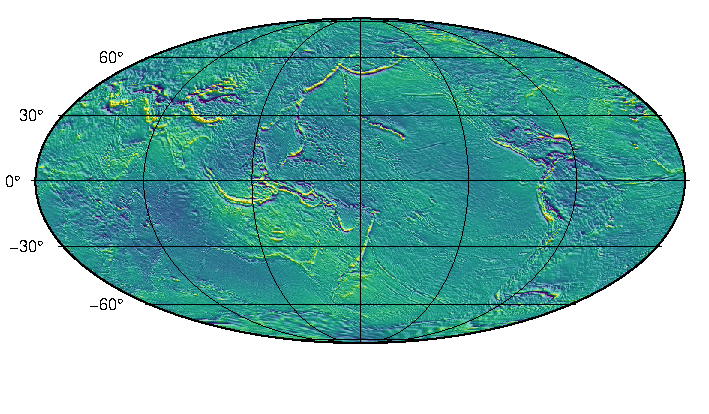
\includegraphics{./fig-gravity-disturbance-on-grs80-x.pdf}
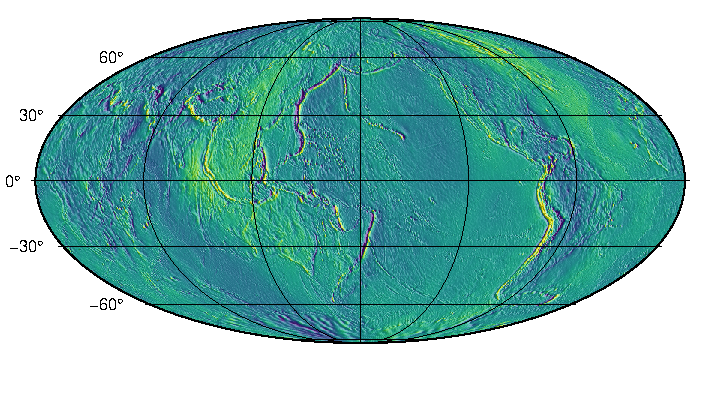
\includegraphics{./fig-gravity-disturbance-on-grs80-y.pdf}
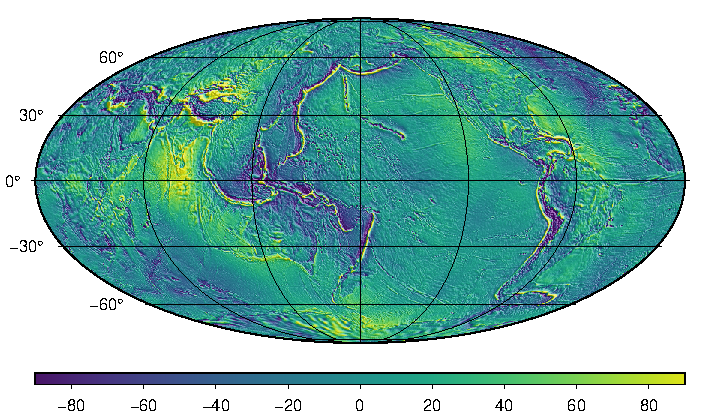
\includegraphics{./fig-gravity-disturbance-on-grs80-z.pdf}
\caption{Prvky vektorovej poruchy tiažového zrýchlenia $\delta 
g_{x^\mathrm{s}}$ (vrchná mapa), $\delta g_{y^\mathrm{s}}$ (prostredná mapa) 
a~$\delta g_{z^\mathrm{s}}$ (spodná mapa) zemského gravitačného poľa vypočítané 
zo sférického harmonického modelu EIGEN-6C4 do stupňa~720 na povrchu 
elipsoidu~GRS80 (jednotky~$\mathrm{mGal}$).  Normálny gravitačný potenciál je 
generovaný ekvipotenciálnym elipsoidom~GRS80.}
\label{fig:dg_ggm_grs80}
\end{figure}

Obrázok~\ref{fig:dg_ggm_450km} znázorňuje prvky poruchy tiažového zrýchlenia vo 
výške~$450$~km nad elipsoidom GRS80.  Z~obrázku je zrejmé, že porucha tiažového 
zrýchlenia sa citeľne vyhladzuje s~narastajúcou vzdialenosťou od Zeme.  Toto 
vyhladzovanie je dokonca rýchlejšie ako v~prípade poruchového potenciálu 
(porovnaj Obrázky~\ref{fig:dg_ggm_grs80} a~\ref{fig:dg_ggm_450km} 
s~Obrázkami~\ref{fig:disturbing_potential_on_grs80} 
a~\ref{fig:disturbing_potential_at_450km}), pretože gravitačné zrýchlenie klesá 
s~druhou mocninou vzdialenosti (rovnica~\ref{eq:gg_body}), zatiaľ čo gravitačný 
potenciál klesá s~prvou mocninou vzdialenosti výpočtového bodu od 
diferenciálneho hmotného elementu (rovnica~\ref{eq:vg_body}).

\begin{figure}
\centering
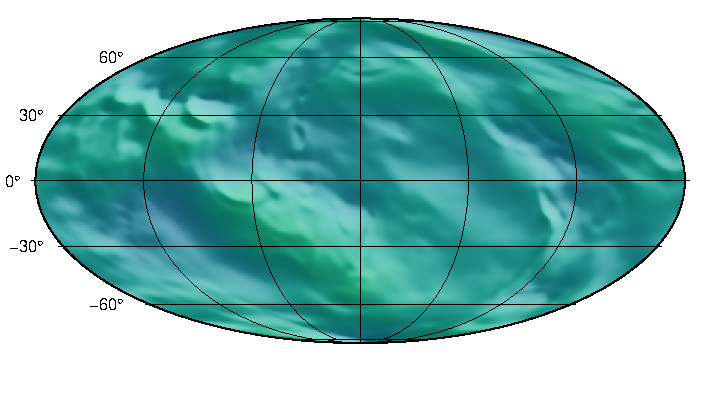
\includegraphics{./fig-gravity-disturbance-at-450km-x.pdf}
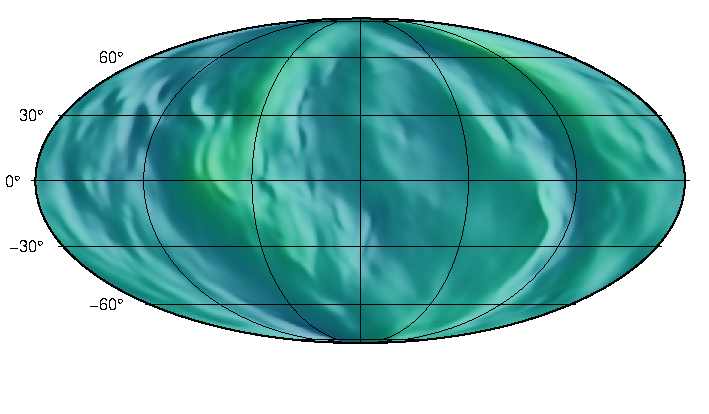
\includegraphics{./fig-gravity-disturbance-at-450km-y.pdf}
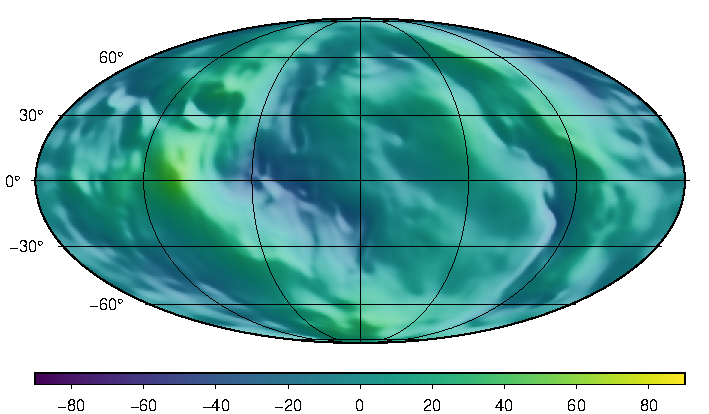
\includegraphics{./fig-gravity-disturbance-at-450km-z.pdf}
\caption{Prvky vektorovej poruchy tiažového zrýchlenia $\delta 
g_{x^\mathrm{s}}$ (vrchná mapa), $\delta g_{y^\mathrm{s}}$ (prostredná mapa) 
a~$\delta g_{z^\mathrm{s}}$ (spodná mapa) získané rovnakým spôsobom ako 
na~Obrázku~\ref{fig:dg_ggm_grs80} avšak vo výške~$450\ \mathrm{km}$ nad 
elipsoidom~GRS80 (jednotky~$\mathrm{mGal}$).  Na oboch obrázkoch je použitá 
rovnaká farebná škála.}
\label{fig:dg_ggm_450km}
\end{figure}

Porucha tiažového zrýchlenia sa spravidla udáva v~jednotke mGal a~nadobúda 
hodnoty v~rozsahu od~$-400\ \mathrm{mGal}$ do $1000\ \mathrm{mGal}$ (hrubý 
odhad na základe modelu~EIGEN-6C4).  Vo fyzikálnej geodézii vystupuje zväčša 
ako meraná veličina, z~ktorej sa snažíme určiť poruchový potenciál a~následne 
priebeh geoidu.  Jedným z~cieľov je preto vyjadriť poruchový potenciál~$T$ 
z~rovníc~(\ref{eq:dg_vector}) a~(\ref{eq:dg_normals}).





\section{Anomália tiažového zrýchlenia}
\label{sec:gravity_anomaly}

Okrem poruchy tiažového zrýchlenia~$\delta \vec g(P)$ 
(Kapitola~\ref{sec:gravity_disturbance}) je s~tiažovým zrýchlením spojená aj 
anomália tiažového zrýchlenia~$\Delta \vec g(P)$.  \emph{Vektorová anomália 
tiažového zrýchlenia} je daná rozdielom skutočného tiažového zrýchlenia~$\vec 
g(P)$ v~bode~$P$ na povrchu Zeme alebo mimo Zeme a~normálneho tiažového 
zrýchlenia~$\boldsymbol\gamma(Q)$ \emph{v~bode~$Q$} 
(Obrázok~\ref{fig:gravity_anomaly}),
%
\begin{equation}
\label{eq:Dg_vector_earth}
\Delta \vec g(P) = \vec g(P) - \boldsymbol\gamma(Q).
\end{equation}

\begin{figure}[bt]
\centering
\input{./fig-gravity-anomaly.pdf_tex}
\caption{Vektorová anomália tiažového zrýchlenia na povrchu Zeme,~$\Delta \vec 
g(P) = \vec g(P) - \boldsymbol \gamma(Q)$, a~na geoide, $\Delta \vec g(P_0) 
= \vec g(P_0) - \boldsymbol\gamma(Q_0)$.  Skutočná tiažnica~$t_W$ a~normálna 
tiažnica~$t_U$ sú z~vizualizačných dôvodov výrazne zakrivené voči normále 
k~elipsoidu~$n_e$.  V~skutočnosti majú~všetky tri línie blízky priebeh.}
\label{fig:gravity_anomaly}
\end{figure}

Bod~$Q$ získame nasledovne.  Nech bodom~$P$ prechádza normálna tiažnica~$t_U$.  
Bod~$Q$ je taký bod na tiažnici~$t_U$, pre ktorý platí~$U(Q) = W(P)$.  
Vzdialenosť medzi bodmi $Q$~a~$P$, ktorá je meraná v~aproximácii po 
normále~$n_e$ namiesto pozdĺž normálnej tiažnice~$t_U$ 
(Obrázok~\ref{fig:gravity_anomaly}), sa nazýva \emph{výšková anomália} a~budeme 
ju označovať symbolom~$\zeta$ (Obrázok~\ref{fig:heights}).  Keď zostrojíme 
výškovú anomáliu pre každý bod na zemskom povrchu, získame plochu, ktorú budeme 
nazývať \emph{teluroid}.  Teluroid predstavuje aproximáciu zemského povrchu.  
Výšková anomália~$\zeta$ nadobúda celosvetovo hodnoty približne od~$-100$~m 
do~$100$~m, podobne ako výška geoidu nad referenčným elipsoidom (pozri 
Kapitolu~\ref{sec:disturbing_field_deflections}).  \emph{Teluroid ale na 
rozdiel od geoidu nie je ekvipotenciálna plocha}.

Dôvod zavedenia anomálie tiažového zrýchlenia je najmä historický.  Ak chceme 
určiť \emph{poruchu tiažového zrýchlenia} v~bode~$P$, potrebné je odmerať 
jednak tiažové zrýchlenie~$g(P)$, ale tiež elipsoidickú šírku a~elipsoidickú 
výšku bodu~$P$.  Znalosť polohy je potrebná kvôli výpočtu normálneho tiažového 
zrýchlenia v~bode merania (Kapitola~\ref{sec:normal_gravity_field}).  
V~súčasnosti už môže byť elipsoidická výška jednoducho odmeraná GNSS metódami.  
V~preddružicovej ére však bolo možné použiť iba niveláciu, ktorou určujeme 
fyzikálne výšky, napríklad výšku definovanú dĺžkou normálnej tiažnice~$t_U$ 
medzi bodmi~$Q_0$ a~$Q$ (Obrázok~\ref{fig:gravity_anomaly}).  Táto výška sa 
nazýva \emph{normálna výška podľa Molodenského}~$H^\mathrm{N}$ 
\parencite{MoritzPhysicalGeodesy}.\footnote{Niveláciou je možné určiť aj iné 
typy fyzikálnych výšok \parencite[pozri][]{MoritzPhysicalGeodesy}.}  Normálne 
tiažové zrýchlenie tak bolo možné vypočítať iba v~bode~$Q$ 
z~výšky~$H^\mathrm{N}$ určenej niveláciou, čím vznikla \emph{anomália tiažového 
zrýchlenia}.  Vzhľadom na súčasnú dostupnosť GNSS je možné očakávať, že 
v~budúcnosti bude vo fyzikálnej geodézii dominovať porucha tiažového zrýchlenia 
\parencite{MoritzPhysicalGeodesy}.  V~súčasnosti sa bežne stretávame s~poruchou 
tiažového zrýchlenia aj s~anomáliou tiažového zrýchlenia.

\begin{figure}[bt]
\centering
\input{./fig-heights.pdf_tex}
\caption{Ortometrická výška~$H^\mathrm{O}$ a~normálna výška podľa 
Molodenského~$H^\mathrm{N}$ merané v~elipsoidickej aproximácii po normále 
k~elipsoidu prechádzajúcej bodom~$P$.  Ortometrická výška~$H^\mathrm{O}$ je 
v~skutočnosti dĺžka skutočnej tiažnice~$t_W$ medzi bodmi~$P_0$ a~$P$ a~normálna 
výška podľa Molodenského je dĺžka normálnej tiažnice~$t_U$ medzi bodmi~$Q_0$ 
a~$Q$ (pozri Obrázok~\ref{fig:gravity_anomaly}).}
\label{fig:heights}
\end{figure}

Hoci vektory~$\vec g$ a~$\boldsymbol\gamma$ sú 
v~rovnici~(\ref{eq:Dg_vector_earth}) dané v~dvoch rôznych bodoch, 
vektor~$\Delta \vec g$ budeme formálne pripisovať bodu~$P$, čomu zodpovedá 
zápis~$\Delta \vec g(P)$.

Vektorová anomália tiažového zrýchlenia môže byť definovaná aj na geoide 
(Obrázok~\ref{fig:gravity_anomaly}),
%
\begin{equation}
\label{eq:Dg_vector_geoid}
\Delta \vec g(P_0) = \vec g(P_0) - \boldsymbol\gamma(Q_0){.}
\end{equation}
%
Aj v~tomto prípade platí rovnosť~$U(Q_0) = W(P_0)$ (pozri 
Kapitolu~\ref{sec:normal_gravity_field}), podobne ako platí rovnosť $U(Q) 
= W(P)$ v~súvislosti s~rovnicou~(\ref{eq:Dg_vector_earth}).  Pre diskusiu 
o~získaní hodnoty tiažového zrýchlenia na geoide $\vec g(P_0)$ pozri 
Kapitolu~\ref{sec:gravity_disturbance}.

Okrem vektorovej anomálie tiažového zrýchlenia sa často stretávame aj so 
\emph{skalárnou anomáliou tiažového zrýchlenia} (pozri tiež 
Kapitolu~\ref{sec:gravity_disturbance}), či už na povrchu Zeme alebo mimo nej,
%
\begin{equation}
\label{eq:Dg_scalar_earth}
\Delta g(P) = \| \vec g(P) \| - \| \boldsymbol \gamma(Q) \| = g(P) 
- \gamma(Q){,}
\end{equation}
%
alebo na geoide,
%
\begin{equation}
\label{eq:Dg_scalar_geoid}
\Delta g(P_0) = \| \vec g(P_0) \| - \| \boldsymbol \gamma(Q_0) \| = g(P_0) 
- \gamma(Q_0){.}
\end{equation}
%
Podobne ako v~súvislosti so skalárnou poruchou tiažového zrýchlenia 
(Kapitola~\ref{sec:gravity_disturbance}), aj tentokrát platí
%
\begin{equation}
\| \Delta \vec g(P) \| \neq \Delta g(P){,}
\end{equation}
%
\begin{equation}
\| \Delta \vec g(P_0) \| \neq \Delta g(P_0){.}
\end{equation}

Anomália tiažového zrýchlenia sa udáva väčšinou v~jednotke~mGal.  Anomália 
a~porucha tiažového zrýchlenia patria medzi základné merateľné veličiny 
fyzikálnej geodézie, z~ktorých určujeme tvar Zeme.  Veličiny~$\Delta \vec 
g(P)$, $\Delta g(P)$, $\delta \vec g(P)$, $\delta g(P)$ sa využívajú prevažne 
na určenie výškovej anomálie~$\zeta$, ktorá je spätá s~normálnou výškou podľa 
Molodenského~$H^\mathrm{N}$.  Veličiny~$\Delta \vec g(P_0)$, $\Delta g(P_0)$, 
$\delta \vec g(P_0)$, $\delta g(P_0)$ sa využívajú najmä na určovanie geoidu, 
ktorý je referenčnou plochou pre \emph{ortometrickú výšku}~$H^\mathrm{O}$ 
(pozri Kapitolu~\ref{sec:orthometric_height}).

\subsection{Vzťah medzi skalárnou anomáliou tiažového zrýchlenia a~poruchovým 
potenciálom}

Nájdime teraz vzťah medzi skalárnou anomáliou tiažového zrýchlenia a~poruchovým 
potenciálom, podobne ako sme našli vzťah medzi skalárnou poruchou tiažového 
zrýchlenia a poruchovým potenciálom (rovnica~\ref{eq:dg_normals}).  Tentokrát 
situáciu komplikuje rozdielna poloha bodov~$P$~a~$Q$, resp.~$P_0$~a~$Q_0$, 
a~zakrivenie normálnej tiažnice (Obrázok~\ref{fig:gravity_anomaly}).  Úlohu si 
výrazne zjednodušíme linearizáciou problému a~využitím elipsoidickej 
aproximácie z~Obrázku~\ref{fig:heights}.  Obe aproximácie sú postačujúce pre 
praktické aplikácie \parencite{MoritzAdvancedGeodesy}.  Následne odvodíme vzťah 
medzi oboma veličinami vo sférickej aproximácii.  Exaktné riešenie bolo nájdené 
v~prácach~\textcite{Meissl1971b} a~\textcite{Borre_chapter8} \parencite[pozri 
tiež napríklad][]{MoritzAdvancedGeodesy,Janak2006}.

\subsubsection{Elipsoidická aproximácia}

Hľadať budeme najprv vzťah medzi~$\Delta g(P_0)$ a~$T(P_0)$ v~bode~$P_0$ na 
geoide.  Rozviňme normálne tiažové zrýchlenie~$\gamma$ v~okolí bodu~$Q_0$ do 
Taylorovho radu a~následne zanedbajme členy druhého a~vyšších rádov, ktorých 
vplyv je malý,
%
\begin{equation}
\label{eq:gamma_P0}
\gamma(P_0) = \sum_{i = 0}^\infty \frac{1}{i!} \, \left.\frac{\partial^i 
\gamma}{\partial h^i}\right|_{Q_0} \, N^i \approx \gamma(Q_0) 
+ \left.\frac{\partial \gamma}{\partial h}\right|_{Q_0} \, N{.}
\end{equation}
%
Dosadením~(\ref{eq:gamma_P0}) do~(\ref{eq:Dg_scalar_geoid}) dostaneme 
v~kombinácii s~(\ref{eq:dg_normals}) vzťah
%
\begin{equation}
\label{eq:Dg_T_tmp}
\begin{split}
\Delta g(P_0) &= g(P_0) - \gamma(P_0) + \left.\frac{\partial \gamma}{\partial 
h}\right|_{Q_0} \, N = \delta g(P_0) + \left.\frac{\partial \gamma}{\partial 
h}\right|_{Q_0} \, N\\
%
&=-\left.\frac{\partial T}{\partial h}\right|_{P_0} + \left.\frac{\partial 
\gamma}{\partial h}\right|_{Q_0} \, N{.}
\end{split}
\end{equation}
%
Rovnica~(\ref{eq:Dg_T_tmp}) popisuje vzťah medzi skalárnou poruchou a~skalárnou 
anomáliou tiažového zrýchlenia v~elipsoidickej aproximácii.  Výšku geoidu nad 
referenčným elipsoidom~$N$ získame rozvojom normálneho tiažového potenciálu~$U$ 
v~okolí bodu~$Q_0$ do Taylorovho radu,
%
\begin{equation}
\label{eq:U_P0}
U(P_0) = \sum_{i = 0}^\infty \frac{1}{i!} \, \left.\frac{\partial^i U}{\partial 
h^i}\right|_{Q_0} \, N^i \approx U(Q_0) + \left.\frac{\partial U}{\partial 
h}\right|_{Q_0} \, N = U(Q_0) - \gamma(Q_0) \, N{.}
\end{equation}
%
S uvážením $W(P_0) = U(Q_0)$ (pozri Kapitolu~\ref{sec:normal_gravity_field}) 
a~vzťahu~(\ref{eq:disturbing_potential}) môžeme prepísať 
rovnicu~(\ref{eq:U_P0}) do tvaru
%
\begin{equation}
\label{eq:N}
N = \frac{T(P_0)}{\gamma(Q_0)}.
\end{equation}
%
Vzťah~(\ref{eq:N}) sa nazýva \emph{Brunsov vzorec} a~umožňuje vypočítať 
\emph{geometrický parameter} (výšku geoidu nad referenčným elipsoidom~$N$) 
\emph{z~fyzikálnych parametrov} (poruchový potenciál~$T(P_0)$ na geoide 
a~normálne tiažové zrýchlenie~$\gamma(Q_0)$ na ekvipotenciálnom elipsoide).  
Brunsov vzorec je základom určovania geoidu.  Dodajme, že zanedbanie členov 
druhého a~vyšších rádov v~rovnici~(\ref{eq:U_P0}) spôsobuje chyby v~určení~$N$ 
na úrovni niekoľko málo milimetrov \parencite{Jekeli2015,Sjoberg2017}, teda 
zhruba o~rád menšie ako je súčasná (približne centimetrová) presnosť určenia 
geoidu.  Je potrebné tiež zdôrazniť, že vzťah~(\ref{eq:N}) bol získaný za 
predpokladu~$U_0 = W_0$.  V~praktickej realizácii je pomerne náročné splniť 
túto podmienku \parencite{MoritzPhysicalGeodesy}.  Preto ak~$U_0 \neq W_0$, 
túto nerovnosť je potrebné zohľadniť v~procese odvodenia vzťahu pre~$N$ (pozri 
napríklad \cite{VanicekGeodesy} alebo \cite{MoritzPhysicalGeodesy}).

Dosadením~(\ref{eq:N}) do~(\ref{eq:Dg_T_tmp}) získame hľadaný vzťah medzi 
anomáliou tiažového zrýchlenia a~poruchovým potenciálom,
%
\begin{equation}
\label{eq:Dg_fundamental_equation_geoid}
\Delta g(P_0) = -\left.\frac{\partial T}{\partial h}\right|_{P_0} 
+ \frac{1}{\gamma(Q_0)} \, \left.\frac{\partial \gamma}{\partial 
h}\right|_{Q_0} \, T(P_0){.}
\end{equation}
%
Rovnica~(\ref{eq:Dg_fundamental_equation_geoid}) sa nazýva \emph{základná 
rovnica fyzikálnej geodézie}.

Podobným spôsobom možno získať základnú rovnicu fyzikálnej geodézie pre 
anomáliu tiažového zrýchlenia na povrchu Zeme alebo mimo Zeme,
%
\begin{equation}
\label{eq:Dg_fundamental_equation_earth}
\begin{split}
\Delta g(P) &= -\left.\frac{\partial T}{\partial h}\right|_{P} 
+ \left.\frac{\partial \gamma}{\partial h}\right|_{Q} \, \zeta\\
%
&= -\left.\frac{\partial T}{\partial h}\right|_{P} + \frac{1}{\gamma(Q)} \, 
\left.\frac{\partial \gamma}{\partial h}\right|_{Q} \, T(P){.}
\end{split}
\end{equation}
%
Na získanie poslednej rovnosti vo 
vzťahu~(\ref{eq:Dg_fundamental_equation_earth}) sme využili \emph{zovšeobecnený 
Brunsov vzorec}
%
\begin{equation}
\label{eq:zeta}
\zeta = \frac{T(P)}{\gamma(Q)}{,}
\end{equation}
%
ktorý je možné získať podobne ako vzťah~(\ref{eq:N}).

Pre kvantifikáciu efektu linearizácie na anomáliu tiažového zrýchlenia pozri 
napríklad \textcite{Claessens2006}.

Je vhodné zdôrazniť, že rôznym bodom~$P$, ktoré sa nachádzajú na povrchu Zeme 
alebo mimo nej a~súčasne ležia na tej istej normále k~elipsoidu, prislúcha 
rozličná hodnota výškovej anomálie~$\zeta$.  Dôvod je ten, že skutočný tiažový 
potenciál~$W(P)$ a~normálny tiažový potenciál~$U(Q)$ klesajú s~narastajúcou 
elipsoidickou výškou rozlične, teda $\left.\frac{\partial W}{\partial 
h}\right|_P \neq \left.\frac{\partial U}{\partial h}\right|_Q$, 
$\left.\frac{\partial^2 W}{\partial h^2}\right|_P \neq \left.\frac{\partial^2 
U}{\partial h^2}\right|_Q$, atď.

\subsubsection{Sférická aproximácia}

Aproximujme deriváciu v~smere elipsoidickej normály~$\partial \slash \partial 
h$ v~rovnici~(\ref{eq:Dg_fundamental_equation_earth}) deriváciou v~smere 
sprievodiča~$\partial \slash \partial r$,
%
\begin{equation}
\Delta g(P) = -\left.\frac{\partial T}{\partial r}\right|_{P} 
+ \frac{1}{\gamma(Q)} \, \left.\frac{\partial \gamma}{\partial r}\right|_{Q} \, 
T(P){.}
\end{equation}
%
V~predošlej rovnici nadobúda člen
%
\begin{equation}
\label{eq:Dg_fundamental_equation_earth_term}
\left.\frac{1}{\gamma(Q)} \, \frac{\partial \gamma}{\partial r}\right|_Q
\end{equation}
%
malé hodnoty.  Kvôli zjednodušeniu matematických vzťahov preto môžeme na jeho 
výpočet využiť gravitačné pole \emph{nerotujúcej} homogénnej gule (alebo 
ekvivalentne hmotného bodu, pozri poznámku 
v~Kapitole~\ref{sec:physical_meaning_of_spherical_harmonic_coefficients}), 
ktoré v~tomto prípade dostatočne presne aproximuje normálne tiažové pole 
ekvipotenciálneho elipsoidu (pozri Kapitolu~\ref{sec:normal_field_ball}).  
Zo~vzťahu pre gravitačný potenciál nerotujúcej homogénnej 
gule~(\ref{eq:vg_ball_out}) potom vyplýva
%
\begin{align}
U &\approx U_g = \frac{GM}{r}{,}\\
%
\gamma &= -\frac{\partial U}{\partial r} = \frac{GM}{r^2}{,}\\
%
\frac{\partial \gamma}{\partial r} &= -2 \, \frac{GM}{r^3}{,}
\end{align}
%
a tak môžeme rovnicu~(\ref{eq:Dg_fundamental_equation_earth_term}) prepísať do 
tvaru
%
\begin{equation}
\left.\frac{1}{\gamma(Q)} \, \frac{\partial \gamma}{\partial r}\right|_Q 
\approx \left.\frac{r^2}{GM} \, \left( -2\frac{GM}{r^3} \right)\right|_Q 
= -\left.\frac{2}{r}\right|_Q {.}
\end{equation}
%
Sférická aproximácia anomálie tiažového zrýchlenia je potom daná vzťahom
%
\begin{equation}
\label{eq:Dg_fundamental_equation_earth_sph}
\Delta g(P) = -\left.\frac{\partial T}{\partial r}\right|_{P} 
- \left.\frac{2}{r}\right|_{P} \, T(P){,}
\end{equation}
%
pričom sme pre zjednodušenie využili približnú rovnosť
%
\begin{equation}
\left.\frac{2}{r}\right|_Q \, T(P) \approx \left.\frac{2}{r}\right|_P \, 
T(P){.}
\end{equation}

Podobným spôsobom získame sférickú aproximáciu skalárnej anomálie tiažového 
zrýchlenia na geoide,
%
\begin{equation}
\label{eq:Dg_fundamental_equation_geoid_sph}
\Delta g(P_0) = -\left.\frac{\partial T}{\partial r}\right|_{P_0} 
- \left.\frac{2}{r}\right|_{P_0} \, T(P_0){.}
\end{equation}

Sférická aproximácia skalárnej anomálie a~skalárnej poruchy tiažového 
zrýchlenia spôsobuje chybu v~určení výšky geoidu nad referenčným elipsoidom~$N$ 
približne na úrovni $0.003 \, N$ \parencite{MoritzPhysicalGeodesy}.  Pri 
dosahovaných hodnotách $N$ zhruba od $-100$ do $100$~m ide o~chybu v~určení 
geoidu na úrovni niekoľkých desatín metra.  V~súčasnosti tak pre presný výpočet 
geoidu už sférická aproximácia nepostačuje.


\subsection{Sférický harmonický rozvoj anomálie tiažového zrýchlenia}

Presný rozvoj anomálie tiažového zrýchlenia do radu sférických harmonických 
funkcií je kvôli zložitosti~jej definície náročný \parencite[pozri 
napríklad][]{Barthelmes2013}.  Uvedieme preto iba rozvoj skalárnej anomálie 
tiažového zrýchlenia vo sférickej aproximácii.  Dosadením~(\ref{eq:t_sh}) 
do~(\ref{eq:Dg_fundamental_equation_earth_sph}) získame
%
\begin{equation}
\label{eq:Dg_sh_sa}
\Delta g(P) = \frac{GM}{R^2} \sum_{n = 0}^\infty (n - 1) \, \left( \frac{R}{r} 
\right)^{n + 2} \sum_{k = -n}^{n} \bar{t}_{nk} \, \bar{Y}_{nk}(\varphi, 
\lambda){.}
\end{equation}
%
Vo sférickej aproximácii sa tak anomália tiažového 
zrýchlenia~(\ref{eq:Dg_sh_sa}) odlišuje od poruchy tiažového 
zrýchlenia~(\ref{eq:dg_sh_sa} a~\ref{eq:dgz_sh}) iba v~člene~$(n - 1)$, ktorý 
nahradil člen~$(n + 1)$.  Všimnime si, že  koeficienty~$\bar{t}_{nk}$ stupňa~$n 
= 1$ neovplyvňujú anomáliu tiažového zrýchlenia v~dôsledku nulového člena~$(n 
- 1)$.

Anomália tiažového zrýchlenia a~porucha tiažového zrýchlenia nadobúdajú podobné 
hodnoty, preto sme vyobrazenie anomálie tiažového zrýchlenia vynechali (pozri 
priebeh poruchy tiažového zrýchlenia na Obrázkoch~\ref{fig:dg_ggm_grs80} 
a~\ref{fig:dg_ggm_450km}).



\subsection*{Dve poznámky k~anomálii tiažového zrýchlenia}

V~súvislosti s~odvodením Brunsovho vzorca a~základnej rovnice fyzikálnej 
geodézie je vhodné opäť zdôrazniť dôležitosť voľby normálneho poľa.  Ak by bolo 
normálne pole zvolené nevhodne, teda rozdiely medzi skutočným a~normálnym poľom 
by s~ohľadom na súčasnú presnosť nemohli byť považované za lineárne, nebolo by 
možné obmedziť rozvoje~(\ref{eq:gamma_P0}) a~(\ref{eq:U_P0}) iba na prvé dva 
členy.  Pridanie už i~len kvadratického člena výrazne komplikuje úlohu.

Druhá poznámka sa týka anomálií tiažového zrýchlenia na geoide~$\Delta g(P_0)$.  
Anomálie tiažového zrýchlenia sú, samozrejme, merané na povrchu Zeme vo 
forme~$\Delta g(P)$ a~na geoid sú redukované až následne matematickými 
metódami.  V~rámci tejto redukcie je potrebné v~prvom kroku matematicky 
odstrániť gravitačný účinok topografických hmôt na tiažové 
zrýchlenie.\footnote{Pre popis redukcie tiažového zrýchlenia na geoid 
s~využitím regularizácie zemského telesa pozri \textcite{Janak2006}.}  Tým 
zabezpečíme jednak to, že v~priestore nad geoidom bude platiť Laplaceova 
rovnica, ale tiež to, že bod~$P$ bude tak povediac visieť vo vzduchu.  Absencia 
hmôt medzi geoidom a~zemským povrchom tak umožní v~ďalšom kroku analyticky 
pokračovať tiažové zrýchlenie nadol z~bodu~$P$ do bodu~$P_0$ (pre analytické 
pokračovanie nadol pozri Kapitolu~\ref{sec:harmonic_function}).  Táto úloha je 
však numericky nestabilná.  To znamená, že v~princípe ju nie je možné vyriešiť 
bez nejakej formy stabilizácie.  Tou môže byť napríklad mierne vyhladenie dát 
či zníženie rozlíšenia daného problému.  Stabilizácia ale spôsobí, že 
v~skutočnosti získame riešenie inej úlohy ako tej, ktorá bola formulovaná 
\parencite{SansoGeodeticBoundaryValueProblem}, hoci získané riešenie môže byť 
rozumne blízke hľadanému riešeniu.  Aby bolo možné potlačiť odchýlky od 
hľadaného riešenia, je potrebné zvyšovať presnosť a~rozlíšenie vstupných 
údajov, čo je v~praktických aplikáciách problematické kvôli náročnosti 
získavania meraných dát.  Redukcia anomálií tiažového zrýchlenia zo zemského 
povrchu na geoid tak patrí medzi najnáročnejšie časti určovania geoidu.





\subsection{Anomálie tiažového zrýchlenia vo voľnom vzduchu a~Bouguerove 
anomálie tiažového zrýchlenia}

Anomália tiažového zrýchlenia, ktorú sme definovali 
vzťahmi~(\ref{eq:Dg_vector_earth}) a~(\ref{eq:Dg_scalar_earth}), sa nazýva 
v~literatúre aj \emph{povrchová anomália tiažového zrýchlenia vo voľnom 
vzduchu} \parencite{SansoGeoidDetermination}.  V~tejto kapitole ju budeme 
označovať symbolom~$\Delta g_{\mathrm{vv}}(P)$.  Okrem nej sa často môžeme 
stretnúť aj s~\emph{anomáliou tiažového zrýchlenia vo voľnom vzduchu na 
geoide}~$\Delta g_{\mathrm{vv}}(P_0)$ a~s~\emph{Bouguerovou anomáliou tiažového 
zrýchlenia}~$\Delta g_{\mathrm{B}}(P)$.  V~tejto kapitole stručne popíšeme nové 
veličiny~$\Delta g_{\mathrm{vv}}(P_0)$ a~$\Delta g_{\mathrm{B}}(P)$.

Na získanie anomálie tiažového zrýchlenia vo voľnom vzduchu na geoide~$\Delta 
g_{\mathrm{vv}}(P_0)$ budeme predpokladať, že nad geoidom nie sú hmoty 
\parencite{MoritzPhysicalGeodesy}.  Bod~$P$ sa teda nachádza \emph{vo voľnom 
vzduchu} (pozri Obrázok~\ref{fig:gravity_anomaly}), a~tak tiažové zrýchlenie 
nad geoidom môžeme rozvinúť do Taylorovho radu.  Po zanedbaní nelineárnych 
členov rozvoja a~po nahradení gradientu skutočného tiažového zrýchlenia 
gradientom normálneho tiažového zrýchlenia získame vzťah
%
\begin{equation}
\label{eq:g_geoid_ts}
g(P) = \sum_{i = 0}^{\infty} \left.\frac{\partial^i g}{\partial 
H^i}\right|_{P_0} \, H^i \approx g(P_0) + \left.\frac{\partial g}{\partial 
H}\right|_{P_0} \, H \approx g(P_0) + \left.\frac{\partial \gamma}{\partial 
h}\right|_{Q_0} \, H = g(P_0) - F{.}
\end{equation}
%
Táto rovnica predstavuje analytické pokračovanie tiažového zrýchlenia nahor 
z~bodu~$P_0$ do bodu~$P$ (pozri Kapitolu~\ref{sec:harmonic_function}).  Tiažové 
zrýchlenie na geoide potom získame vzťahom
%
\begin{equation}
\label{eq:Dgvv_gP0}
g(P_0) \approx g(P) + F{,}
\end{equation}
%
ktorý reprezentuje analytické pokračovanie tiažového zrýchlenia nadol 
z~bodu~$P$ do bodu~$P_0$.\footnote{\label{fn:Dgvv_P0_dc}Je vhodné pripomenúť, 
že analytické pokračovanie \emph{nadol} je numericky nestabilná úloha (pozri 
Kapitolu~\ref{sec:harmonic_function}).  Stabilizácia je v~tomto prípade 
vykonaná zanedbaním nelineárnych členov Taylorovho 
rozvoja~(\ref{eq:g_geoid_ts}) a~nahradením gradientu~$\left.\frac{\partial 
g}{\partial H}\right|_{P_0}$ gradientom~$\left.\frac{\partial \gamma}{\partial 
h}\right|_{Q_0}$.  Pre diskusiu o~presnosti aproximácie~$\frac{\partial 
g}{\partial H} \approx \frac{\partial \gamma}{\partial h}$ pozri 
Kapitolu~\ref{sec:normal_gravity_taylor_expansion}.}  Člen~$F$ teda 
\emph{približne} redukuje skutočné tiažové zrýchlenie z~bodu~$P$ na povrchu 
Zeme do bodu~$P_0$ na geoide.  Použitím rovníc~(\ref{eq:Dg_scalar_geoid}) 
a~(\ref{eq:Dgvv_gP0}) získame výsledný vzťah pre anomáliu tiažového zrýchlenia 
vo voľnom vzduchu na geoide
%
\begin{equation}
\label{eq:Dgvv_geoid_ts}
\Delta g_\mathrm{vv}(P_0) = g(P) + F - \gamma(Q_0){.}
\end{equation}
%
Kvôli nízkej presnosti sa rovnica~(\ref{eq:Dgvv_geoid_ts}) už v~súčasnosti 
prakticky nepoužíva.

Druhá veličina, \emph{Bouguerova anomália tiažového zrýchlenia}~$\Delta 
g_{\mathrm{B}}(P)$ \parencite{MoritzPhysicalGeodesy}, získala názov po 
P.~Bouguerovi (1698~-- 1758), francúzskom matematikovi, geofyzikovi, geodetovi 
a~astronómovi.  Využíva sa najmä v~geofyzike na detekciu podpovrchových 
hustotných kontrastov.  Na jej získanie je potrebné vypočítať gravitačný účinok 
topografických hmôt\footnote{Definícia pojmu topografické hmoty sa nachádza na 
strane~\pageref{def:topographic_masses}.} na tiažové zrýchlenie a~odstrániť ho 
z~povrchovej anomálie tiažového zrýchlenia.  Bouguerove anomálie tak majú 
výrazne hladší priebeh ako povrchové anomálie, ktoré sú veľmi závislé od 
lokálnych hmôt.  V~geodézii často využívame hladký priebeh Bouguerových 
anomálií nasledovným spôsobom.  Povrchové anomálie tiažového zrýchlenia vo 
voľnom vzduchu sú v~teréne odmerané spravidla v~sieti priestorovo nepravidelne 
rozmiestnených bodov.  Na numericky efektívne určovanie tvaru Zeme je ale 
výhodné, aby dáta boli dostupné v~pravidelnej sieti bodov.  Často je preto 
potrebné interpolovať povrchové anomálie do pravidelnej siete bodov.  Povrchové 
anomálie majú ale komplikovaný priebeh, podobne ako samotný zemský povrch, 
preto nie sú vhodné na interpoláciu.  Namiesto toho môžeme v~bodoch 
nepravidelnej siete vypočítať najprv Bouguerove anomálie a~tie následne 
interpolovať do pravidelnej siete bodov.  Vďaka hladkému priebehu Bouguerových 
anomálii sa takouto interpoláciou dopustíme menších chýb, ako keby sme 
interpolovali priamo povrchové anomálie.  Povrchové anomálie napokon získame 
v~bodoch pravidelnej siete spätným výpočtom z~interpolovaných Bouguerových 
anomálií.  V~geodézii sa teda Bouguerove anomálie využívajú najmä ako pomocná 
veličina.

Bližšie podrobnosti o~gravitačnom účinku topografických hmôt, o~anomáliách 
tiažového zrýchlenia, o~Bouguerových anomáliách tiažového zrýchlenia a~o~ich 
historickom pozadí je možné nájsť napríklad v~publikáciách 
\textcite{Meurers2017}, \textcite{Mikuska2017} a~\textcite{Vajda2020}.





\section{Zvislicové odchýlky}
\label{sec:deflections}

V~Kapitolách~\ref{sec:gravity_disturbance} a~\ref{sec:gravity_anomaly} sme 
videli, že jedna z~merateľných veličín fyzikálnej geodézie, tiažové zrýchlenie, 
súvisí s~poruchovým potenciálom, a~teda aj s~určovaným tvarom Zeme (pozri 
rovnicu~\ref{eq:N}).  Medzi časté geodetické merania ale patrí aj určovanie 
polohy bodu na povrchu Zeme pomocou astronomických a~GNSS meraní.  Je preto 
výhodné nájsť vzťah aj medzi týmito meraniami a~poruchovým potenciálom, pretože 
nám to umožní určovať tvar Zeme z~ďalšieho typu geodetických dát.  Hoci to na 
prvý pohľad nemusí byť zrejmé, takýto vzťah naozaj existuje.  Na jeho nájdenie 
zavedieme veličinu, ktorú budeme nazývať zvislicová odchýlka.

\emph{Zvislicová odchýlka} je uhol medzi skutočnou zvislicou (pozri 
Kapitolu~\ref{sec:plumbline}) a~zvoleným referenčným smerom 
\parencite{TorgeGeodesy}.  Referenčný smer často závisí od aplikácie, preto sa 
v~literatúre môžeme stretnúť s~rozličnými definíciami zvislicových odchýlok 
(Obrázok~\ref{fig:deflections}).

\begin{figure}[bt]
\centering
\input{./fig-deflections.pdf_tex}
\caption{Helmertova zvislicová odchýlka~$\Theta^\textrm{Helmert}$, Molodenského 
zvislicová odchýlka~$\Theta^\textrm{Molodenskij}$ a~Pizzettiho zvislicová 
odchýlka~$\Theta^\textrm{Pizzetti}$.  Symbol~$t_W^P$ označuje skutočnú tiažnicu 
prechádzajúcu bodom~$P$ na povrchu Zeme.  Tiažnica~$t_W^P$ je identická so 
skutočnou tiažnicou~$t_W^{P_0}$, ktorá prechádza bodom~$P_0$ na geoide.  
Symboly~$z_W^P$ a~$z_W^{P_0}$ označujú skutočné zvislice v~bodoch~$P$ a~$P_0$.  
Zvislicou rozumieme dotyčnicu k~tiažnici, v~tomto prípade v~bodoch~$P$ a~$P_0$ 
(pozri Kapitolu~\ref{sec:plumbline}).  Symbol~$n$ označuje normálu, pričom 
dolný index označuje plochu, na ktorú je normála kolmá ($e$ pre elipsoid, $U$ 
pre normálnu ekvipotenciálnu plochu~$U = \textrm{kon\v{s}t.}$), a~horný index 
označuje bod, cez ktorý normála prechádza.  Poznamenajme, že normála~$n_U^P$ 
nie je totožná s~\emph{normálnou} zvislicou~$z_U^Q$, hoci sú si veľmi blízke.}
\label{fig:deflections}
\end{figure}

\begin{itemize}
\item \emph{Helmertova zvislicová odchýlka}~$\Theta^\mathrm{Helmert}$ je uhol 
medzi skutočnou zvislicou~$z_W^P$ prechádzajúcou~bodom~$P$ na povrchu Zeme 
a~normálou k~elipsoidu~$n_e^P$ prechádzajúcou bodom~$P$.  Táto zvislicová 
odchýlka sa tiež zvykne nazývať \textit{astronomicko--geodetická zvislicová 
odchýlka} \parencite{Jekeli1999b}.

\item \emph{Molodenského zvislicová odchýlka}~$\Theta^\mathrm{Molodenskij}$ je 
uhol medzi skutočnou zvislicou~$z_W^P$ prechádzajúcou bodom~$P$ na povrchu Zeme 
alebo mimo nej a~normálou~$n_U^P$ k~takej normálnej ekvipotenciálnej 
ploche~$U(Q) = \textrm{kon\v{s}t.}$, ktorej normálny tiažový potenciál~$U(Q)$ 
je rovný skutočnému tiažovému potenciálu~$W(P)$, pričom normála~$n_U^P$ 
prechádza bodom~$P$.

\item \emph{Pizzettiho zvislicová odchýlka}~$\Theta^\mathrm{Pizzetti}$ je uhol 
medzi skutočnou zvislicou~$z_W^{P_0}$ prechádzajúcou bodom~$P_0$ na povrchu 
geoidu a~normálou k~elipsoidu~$n_e^{P_0}$ prechádzajúcou bodom~$P_0$.

\item \emph{Gravimetrická zvislicová odchýlka}~$\Theta^\mathrm{grav}$ je uhol 
medzi vektormi~$\vec g(P)$ a~$\boldsymbol\gamma(P)$ v~bode~$P$ na povrchu Zeme 
alebo~mimo nej (Obrázok~\ref{fig:gravity_disturbance}).\footnote{Vzhľadom na 
malé zakrivenie normálnej tiažnice a~vzhľadom na krátku vzdialenosť medzi 
bodmi~$P$~a~$Q$ je uhol medzi vektormi~$\vec g(P)$ a~$\boldsymbol\gamma(Q)$ 
(Obrázok~\ref{fig:gravity_anomaly}) veľmi podobný uhlu medzi vektormi~$\vec 
g(P)$~a~$\boldsymbol\gamma(P)$ (Obrázok~\ref{fig:gravity_disturbance}).  
V~mnohých situáciách preto nie je potrebné rozlišovať, či gravimetrická 
zvislicová odchýlka je daná vektormi~$\vec g(P)$~a~$\boldsymbol\gamma(P)$ 
alebo~$\vec g(P)$~a~$\boldsymbol\gamma(Q)$.}  Po regularizácii zemského telesa 
(Kapitola~\ref{sec:disturbing_potential}) je možné definovať gravimetrické 
zvislicové odchýlky aj na geoide a v~jeho vonkajšom priestore.
\end{itemize}
%
Rozdiel medzi Helmertovou a~Molodenského zvislicovou odchýlkou je spôsobený 
zakrivením normálnej tiažnice \parencite{Jekeli1999b}.  Zvislicové 
odchýlky~$\Theta$ nadobúdajú hodnoty od $0$ v~rovinatom teréne do 
približne~$2'$ v~blízkosti najväčších pohorí na Zemi \parencite{GGMplus}, 
zvyčajne však najviac niekoľko desiatok uhlových sekúnd.

Nech je daný súradnicový systém, v~ktorom je smer skutočnej zvislice daný 
astronomickými súradnicami~$\Phi$ a~$\Lambda$.  Nech je ďalej daný referenčný 
elipsoid, voči ktorému sú určované súradnice~$\Phi^{\mathrm{Ref}}$ 
a~$\Lambda^{\mathrm{Ref}}$ (napríklad sférické alebo elipsoidické) referenčného 
smeru zvislicovej odchýlky.  Predpokladajme, že osi~$z$ oboch súradnicových 
systémov sú rovnobežné a~rovnako tak sú rovnobežné aj roviny ich nultých 
poludníkov \parencite{TorgeGeodesy}.\footnote{Súčasné súradnicové systémy 
zabezpečujú splnenie týchto podmienok s~dostatočnou presnosťou.  Riešenie pre 
súradnicové systémy, ktoré tieto podmienky nespĺňajú, je možné nájsť napríklad 
v~práci \textcite{Pick2000}.}  Rovnobežným posunutím takýchto súradnicových 
systémov do bodu~$P$, v~ktorom určujeme zvislicovú odchýlku, získame situáciu 
znázornenú na Obrázku~\ref{fig:deflections_unit_sphere}.

Zvislicovú odchýlku je možné popísať rozličnými spôsobmi, z~ktorých dva sú 
obzvlášť výhodné (Obrázok~\ref{fig:deflections_unit_sphere}).  Jeden využíva 
veľkosť uhlového vychýlenia~$\Theta$ medzi skutočnou zvislicou a~referenčným 
smerom a~azimut~$\alpha$, ktorý udáva smer vychýlenia v~rovine lokálneho 
horizontu.  Druhý prístup rozkladá zvislicovú odchýlku do dvoch kolmých smerov.  
Jedna zložka popisuje priemet zvislicovej odchýlky do~roviny meridiánu; budeme 
ju označovať symbolom~$\xi$.  Druhá zložka popisuje priemet zvislicovej 
odchýlky do~roviny prvého vertikálu; označovať ju budeme symbolom~$\eta$.

\begin{figure}[bt]
\centering
\input{./fig-deflections-unit-sphere.pdf_tex}
\caption{Vektor zvislicovej odchýlky~$\boldsymbol\Theta$ na jednotkovej sfére 
so stredom v~bode~$P$, v~ktorom je určovaná zvislicová odchýlka.  Zvislicová 
odchýlka je znázornená v~podobe 1)~veľkosti~$\Theta = \| \boldsymbol\Theta \|$ 
a~azimutu~$\alpha$ a~2)~pravouhlých priemetov~$\xi$ a~$\eta$ do meridiánovej 
roviny a~do roviny prvého vertikálu.  Symboly~$\Phi$ a~$\Lambda$ označujú 
astronomické súradnice bodu~$P$, v~ktorom je určovaná zvislicová odchýlka 
(pozri Obrázok~\ref{fig:deflections}).  Symboly~$\phi$ a~$\lambda$ označujú 
elipsoidickú šírku a~elipsoidickú dĺžku bodu~$P$.  Referenčným smerom na~tomto 
obrázku je teda normála k~elipsoidu, ktorá prechádza bodom~$P$.}
\label{fig:deflections_unit_sphere}
\end{figure}

Zložky~$\xi$ a~$\eta$ získame z~Obrázku~\ref{fig:deflections_unit_sphere},
%
\begin{equation}
\begin{split}
\xi  &= \Phi - \phi{,}\\
\eta &= (\Lambda - \lambda) \, \cos\phi{.}
\end{split}
\end{equation}
%
Veľkosť zvislicovej odchýlky~$\Theta$ môžeme vypočítať sférickou kosínusovou 
vetou vo sférickom trojuholníku~$N$, $N_r$ a~$N'_r$ 
(Obrázok~\ref{fig:deflections_unit_sphere}).  Keďže ale uhly~$\Theta$, $\xi$ 
a~$\eta$ nadobúdajú malé hodnoty (v~absolútnej hodnote nanajvýš približne 
$2'$), s~dostatočnou presnosťou môžeme použiť kosínusovú vetu pre rovinný 
trojuholník,
%
\begin{equation}
\label{eq:deflection_total}
\Theta \approx \sqrt{\xi^2 + \eta^2 - 2\, \xi \, \eta \, \cos 90^{\circ}} 
= \sqrt{\xi^2 + \eta^2}{.}
\end{equation}
%
Použitím vzťahov sférickej trigonometrie 
\parencite[napríklad][]{MoritzPhysicalGeodesy},
%
\begin{equation}
\label{eq:deflection_aux}
\begin{split}
\sin\Theta \, \cos\alpha &= \cos\phi \, \sin\Phi - \sin\phi \, \cos\Phi \, 
\cos(\Lambda - \lambda){,}\\
\sin\Theta \, \sin\alpha &= \cos\Phi \, \sin(\Lambda - \lambda),
\end{split}
\end{equation}
%
získame azimut zvislicovej odchýlky 
(Obrázok~\ref{fig:deflections_unit_sphere}),
%
\begin{equation}
\label{eq:deflection_azimuth}
\tan\alpha = \frac{\cos\Phi \, \sin(\Lambda - \lambda)}{\cos\phi \, \sin\Phi 
- \sin\phi \, \cos\Phi \, \cos(\Lambda - \lambda)}{.}
\end{equation}
%
Zvislicovú odchýlku môžeme chápať aj ako dvojrozmerný rovinný 
vektor~$\boldsymbol\Theta = [\xi, \eta]^\top$, ktorý má veľkosť~$\Theta = \| 
\boldsymbol\Theta \|$ (rovnica~\ref{eq:deflection_total}) a~smer~$\alpha$ 
(rovnica~\ref{eq:deflection_azimuth}).  Pomocou známej hodnoty meridiánovej 
a~priečnej zložky zvislicovej odchýlky tiež môžeme zvislicovú odchýlku 
premietnuť do ľubovoľného smeru, ktorý je daný azimutom~$A$ 
(Obrázok~\ref{fig:deflections_projection}),
%
\begin{equation}
\label{eq:deflection_vareps}
\varepsilon = \xi \, \cos A + \eta \, \sin A{.}
\end{equation}


\begin{figure}[bt]
\centering
\input{./fig-deflections-projection.pdf_tex}
\caption{Priemet zvislicovej odchýlky~$\Theta = [\xi, \eta]^\top$ v~bode~$P$ do 
spojnice s~azimutom~$A$ v~rovinnej aproximácii.}
\label{fig:deflections_projection}
\end{figure}

Okrem určovania tvaru Zeme majú zvislicové odchýlky praktické využitie aj 
v~ďalších geodetických úlohách.  Geodetické prístroje ako teodolit či nivelačný 
prístroj sa horizontujú preto, aby sa ich vertikálna os stotožnila so skutočnou 
zvislicou.  Merané vodorovné smery, vertikálne uhly či vertikálne prevýšenia sú 
tak vztiahnuté k~skutočnej zvislici, resp. skutočnému lokálnemu horizontu.  
Skutočné zvislice prechádzajúce dvoma rôznymi bodmi nie sú ale vo všeobecnosti 
rovnobežné, preto niektoré geodetické merania si môžu vyžadovať korekciu týchto 
efektov, obzvlášť ak je vyžadovaná presnosť vysoká.  Na výpočet takýto korekcii 
slúžia práve zvislicové odchýlky.  Ďalšie využitie zvislicových odchýlok je 
napríklad na navigáciu inerciálnych navigačných systémov \parencite[pozri 
napríklad][]{Jekeli2000}.


\subsection{Vzťah medzi zvislicovou odchýlkou a~poruchovým potenciálom}
\label{sec:deflections_disturbing_potential}

Na získanie vzťahu medzi zvislicovými odchýlkami a~poruchovým potenciálom 
budeme uvažovať gravimetrickú zvislicovú odchýlku pre jej priamočiaru súvislosť 
s~tiažovým poľom.  V~tejto kapitole budeme pre jednoduchosť označovať 
zvislicové odchýlky a~ich zložky symbolmi~$\Theta$, $\xi$, $\eta$ bez horného 
indexu.  Zvislicové odchýlky budeme určovať na povrchu Zeme alebo mimo nej 
v~bode~$P$.  Po regularizácii zemského telesa 
(Kapitola~\ref{sec:disturbing_potential}) je možné získať rovnaké vzťahy aj pre 
zvislicové odchýlky na geoide a~mimo neho.

Gravimetrickú zvislicovú odchýlku sme definovali ako uhol medzi skutočnou 
a~normálnou zvislicou v~bode~$P$.  Keďže smer zvislice je totožný so smerom 
normály k~ekvipotenciálnej ploche, trojrozmerný vektor zvislicovej odchýlky je 
daný vzťahom \parencite{SansoGeoidDetermination},
%
\begin{equation}
\label{eq:deflection_eps}
\boldsymbol\varepsilon(P) = \vec n_W(P) - \vec n_U(P){,}
\end{equation}
%
kde $\vec n_W(P)$ a~$\vec n_U(P)$ sú jednotkové vektory \emph{vonkajších} 
normál ku~skutočnej a~normálnej ekvipotenciálnej ploche v~bode~$P$ (pozri 
Obrázok~\ref{fig:gravity_disturbance}).  Horizontálne zložky~$\varepsilon_x$, 
$\varepsilon_y$ vektora~$\boldsymbol\varepsilon = [\varepsilon_x, 
\varepsilon_y, \varepsilon_z]^\top$ predstavujú zložky~$\xi$ a~$\eta$ 
vektora~$\boldsymbol\Theta = [\xi, \eta]^\top$ (pozri 
Kapitolu~\ref{sec:deflections}), teda
%
\begin{equation}
\label{eq:xi_eta_eps}
\begin{split}
\xi = \varepsilon_x{,}\\
\eta = \varepsilon_y{.}
\end{split}
\end{equation}

Z~definície operátora gradient vyplýva, že jednotkové vektory~$\vec n_W(P)$ 
a~$\vec n_U(P)$ sú dané vzťahmi
%
\begin{equation}
\label{eq:nw_nu}
\begin{split}
\vec n_W(P) &= -\frac{\nabla W(P)}{\| \nabla W(P) \|} = -\frac{\nabla 
W(P)}{g(P)}{,}\\
%
\vec n_U(P) &= -\frac{\nabla U(P)}{\| \nabla U(P) \|} = -\frac{\nabla 
U(P)}{\gamma(P)}{.}
\end{split}
\end{equation}
%
Po dosadení do vzťahu~(\ref{eq:deflection_eps}) tak získame rovnicu
%
\begin{equation}
\label{eq:deflection_eps2}
\boldsymbol\varepsilon(P) = -\frac{\nabla W(P)}{g(P)} + \frac{\nabla 
U(P)}{\gamma(P)}{.}
\end{equation}
%
S~využitím vzťahov~(\ref{eq:gradient_additivity}), 
(\ref{eq:disturbing_potential}),  (\ref{eq:dg_scalar}) a~(\ref{eq:nw_nu}) 
môžeme ďalej upraviť túto rovnicu do tvaru
%
\begin{equation}
\label{eq:deflection_eps3}
\begin{split}
\boldsymbol\varepsilon(P) &= - \frac{\nabla W(P) - \nabla U(P)}{\gamma(P)} 
- \frac{\gamma(P) - g(P)}{\gamma(P)} \, \frac{\nabla W(P)}{g(P)}\\
%
&= - \frac{\nabla T(P)}{\gamma(P)} + \frac{\delta g(P)}{\gamma(P)} \,  \, 
\frac{\nabla W(P)}{g(P)}\\
%
&= - \frac{\nabla T(P)}{\gamma(P)} - \frac{\delta g(P)}{\gamma(P)} \, \vec 
n_W(P){.}\\
\end{split}
\end{equation}
%
Po uvážení~(\ref{eq:xi_eta_eps}) tak získame vzťahy
%
\begin{equation}
\label{eq:deflection_grav}
\begin{split}
\xi &= -\frac{1}{\gamma(P)} \, \left.\frac{\partial T}{\partial x}\right|_{P} 
+ \frac{1}{g(P)} \, \frac{\delta g(P)}{\gamma(P)} \, \left.\frac{\partial 
W}{\partial x}\right|_P = -\frac{T_x(P)}{\gamma(P)} + \frac{\delta 
g(P)}{\gamma(P)} \, \frac{W_x(P)}{g(P)}{,}\\
%
\eta &= -\frac{1}{\gamma(P)} \, \left.\frac{\partial T}{\partial y}\right|_{P} 
+ \frac{1}{g(P)} \, \frac{\delta g(P)}{\gamma(P)} \, \left.\frac{\partial 
W}{\partial y}\right|_P= -\frac{T_y(P)}{\gamma(P)} + \frac{\delta 
g(P)}{\gamma(P)} \, \frac{W_y(P)}{g(P)}{.}\\
\end{split}
\end{equation}
%
Rovnica~(\ref{eq:deflection_grav}) popisuje vzťah medzi lokálnymi 
charakteristikami tiažového poľa v~bode~$P$ na jednej strane a~zvislicovými 
odchýlkami v~bode~$P$ na strane druhej.

Zložky~$\varepsilon_x$ a~$\varepsilon_y$ z~rovnice~(\ref{eq:xi_eta_eps}) sme 
zámerne opísali vágnym prívlastkom \emph{horizontálne} bez toho, aby sme 
bližšie špecifikovali, na ktorú zvislicu či normálu je horizontálna rovina 
kolmá (pozri Obrázok~\ref{fig:deflections}).  Voľba horizontálnej roviny môže 
byť totiž vynútená okolnosťami, a~tak sa môžeme stretnúť s~rozličnými tvarmi 
rovnice~(\ref{eq:deflection_grav}).  Definujme lokálny karteziánsky súradnicový 
systém~$x^\mathrm{a}, y^\mathrm{a}, z^\mathrm{a}$ s~pohyblivým začiatkom 
v~bode~$P$ nasledovne.  Os~$z^\mathrm{a}$ je daná smerom skutočnej zvislice 
v~bode~$P$ (pozri~$z_W^P$ na Obrázku~\ref{fig:deflections}) a~je orientovaná 
kladne vo vonkajšom smere.  Os~$x^\mathrm{a}$ leží v~rovine meridiánu a~je 
orientovaná kladne na sever.  Os~$y^\mathrm{a}$ dotvára pravouhlý 
\emph{ľavotočivý} súradnicový systém.  Horizontálna 
rovina~$x^\mathrm{a}y^\mathrm{a}$ je teda kolmá na vektor~$\vec n_W(P)$, preto 
$W_{x^\mathrm{a}}(P) = W_{y^\mathrm{a}}(P) = 0$.  
Rovnice~(\ref{eq:deflection_grav}) potom prejdú do tvaru 
\parencite{Borre_chapter4}
%
\begin{equation}
\label{eq:deflection_grav_nat}
\begin{split}
\xi &= -\frac{T_{x^\mathrm{a}}(P)}{\gamma(P)}{,}\\
%
\eta &= -\frac{T_{y^\mathrm{a}}(P)}{\gamma(P)}{.}
\end{split}
\end{equation}
%
V~praktických výpočtoch sa ale tieto vzťahy použivajú zriedkavo, pretože 
vyžadujú znalosť smeru skutočnej zvislice v~bode~$P$ 
(Obrázok~\ref{fig:deflections}).  Ten je možné získať určením astronomických 
súradníc~$\Phi, \Lambda$ bodu~$P$.

V~praxi sa horizontálna rovina zvykne voliť tak, aby bola kolmá na normálu 
k~elipsoidu~$n_e^P$ (pozri Obrázok~\ref{fig:deflections}).  Definujme teda 
lokálny karteziánsky súradnicový systém~$x^\mathrm{e}, y^\mathrm{e}, 
z^\mathrm{e}$ s~pohyblivým začiatkom v~bode~$P$ podobne ako súradnicový 
systém~$x^\mathrm{a}, y^\mathrm{a}, z^\mathrm{a}$, avšak s~tým rozdielom, že 
os~$z^\mathrm{e}$ je tentokrát daná smerom normály k~elipsoidu~$n_e^P$.  
Rovina~$x^\mathrm{e}y^{\mathrm{e}}$ je tak kolmá na normálu~$n^P_{\mathrm{e}}$ 
a~prechádza bodom~$P$.  Horizontálne zložky vektora~$\boldsymbol\varepsilon$ 
v~rovine~$x^\mathrm{e}y^\mathrm{e}$ predstavujú \emph{elipsoidickú aproximáciu} 
gravimetrickej zvislicovej odchýlky \parencite{Jekeli1999b},
%
\begin{equation}
\label{eq:deflection_grav_e}
\begin{split}
\xi &\approx -\frac{1}{\gamma(P)} \, \left.\frac{\partial T}{(M + h) \, 
\partial \phi}\right|_P{,}\\
%
\eta &\approx -\frac{1}{\gamma(P)} \, \left.\frac{\partial T}{(N + h) \, 
\cos\phi \, \partial \lambda}\right|_P{.}
\end{split}
\end{equation}
%
V~rovnici~(\ref{eq:deflection_grav_e}) označuje symbol~$M$ meridiánový polomer 
krivosti \parencite{TorgeGeodesy},
%
\begin{equation}
M = \frac{a \, (1 - e^2)}{\left(1 - e^2 \, \sin^2\phi \right)^{3 \slash 2}}{,}
\end{equation}
%
$N$ označuje priečny polomer krivosti (rovnica~\ref{eq:curvature_N}) a~$\phi$ 
je elipsoidická šírka (Kapitola~\ref{sec:ellipsoidal_height}).  Približný 
charakter rovníc~(\ref{eq:deflection_grav_e}) je spôsobený zanedbaním 
členov~$\frac{\delta g(P)}{\gamma(P)} \, \frac{W_{x^\mathrm{e}}(P)}{g(P)}$ 
a~$\frac{\delta g(P)}{\gamma(P)} \, \frac{W_{y^\mathrm{e}}(P)}{g(P)}$ 
(pozri~\ref{eq:deflection_grav}).  Ich vplyv však nepresahuje zhruba $0.5''$ 
pre zložku~$\xi$ a~$0.1''$ pre zložku~$\eta$ (hrubý odhad pomocou modelu 
EIGEN-6C4).  Maximálna chyba zo zanedbania týchto členov je väčšia 
v~zložke~$\xi$ ako v~zložke~$\eta$, pretože $\max(|W_{x^\mathrm{e}}|) 
> \max(|W_{y^\mathrm{e}}|)$ v~dôsledku významného trendu 
v~člene~$W_{x^\mathrm{e}}$, ktorý je spôsobený sploštením Zeme v~smere 
elipsoidickej šírky.

V~praktických aplikáciách je niekedy potrebné vykonať ďalšie priblíženie 
rovnice~(\ref{eq:deflection_grav_e}) zavedením \emph{sférickej aproximácie}.  
Jeden z~dôvodov je ten, že poruchový potenciál~$T$ 
z~rovnice~(\ref{eq:deflection_grav_e}) je veľmi často aproximovaný sférickým 
harmonickým rozvojom~(\ref{eq:t_sh}).  Výpočet parciálnej derivácie poruchového 
potenciálu podľa elipsoidickej šírky~$\phi$ je potom náročný, pretože 
rozvoj~(\ref{eq:t_sh}) je vyjadrený pomocou sférickej šírky~$\varphi$ 
(elipsoidická a~sférická dĺžka sú totožné).\footnote{Pre vzťah na výpočet 
derivácie $\frac{1}{M + h} \, \frac{\partial}{\partial\phi}$ pomocou sférických 
derivácií~$\frac{1}{r} \, \frac{\partial}{\partial \varphi}$ 
a~$\frac{\partial}{\partial r}$ pozri napríklad publikáciu 
\textcite{Jekeli1999b}.}  Uvažujme teraz súradnicový systém~$x^\mathrm{s}, 
y^\mathrm{s}, z^\mathrm{s}$ z~Obrázku~\ref{fig:cart_sph} a~jeho horizontálnu 
rovinu~$x^\mathrm{s}y^\mathrm{s}$.  Sférická aproximácia gravimetrických 
zvislicových odchýlok má tvar \parencite{Jekeli1999b}
%
\begin{equation}
\label{eq:deflection_grav_s}
\begin{split}
\xi &\approx -\frac{1}{\gamma(P)} \, \frac{1}{r} \, \left.\frac{\partial 
T}{\partial \varphi}\right|_P = -\frac{\delta 
g_{x^\mathrm{s}}(P)}{\gamma(P)}{,}\\
%
\eta &\approx -\frac{1}{\gamma(P)} \, \frac{1}{r \, \cos\varphi} \, 
\left.\frac{\partial T}{\partial \lambda}\right|_P = -\frac{\delta 
g_{y^\mathrm{s}}(P)}{\gamma(P)}{,}
\end{split}
\end{equation}
%
pretože z~Prílohy~\ref{app:gradient_in_spherical_coordinates} vieme, že 
horizontálne derivácie v~súradnicovom systéme~$x^\mathrm{s}, y^\mathrm{s}, 
z^\mathrm{s}$ sú dané vzťahmi~$\frac{\partial}{\partial x^\mathrm{s}} 
= \frac{1}{r} \, \frac{\partial}{\partial\varphi}$ a~$\frac{\partial}{\partial 
y^\mathrm{s}} = \frac{1}{r \, \cos\varphi} \, 
\frac{\partial}{\partial\lambda}$.  Chyba spôsobená zanedbaním 
člena~$\frac{\delta g(P)}{\gamma(P)} \, \frac{W_{x^\mathrm{s}}(P)}{g(P)}$ 
z~rovnice~(\ref{eq:deflection_grav}) dosahuje približne~$0.8''$ pre~$\xi$.  
Chyba v~dôsledku zanedbania člena~$\frac{\delta g(P)}{\gamma(P)} \, 
\frac{W_{y^\mathrm{s}}(P)}{g(P)}$ je rovnaká ako v~prípade elipsoidickej 
aproximácie, pretože $y^\mathrm{s} = y^\mathrm{e}$.  Pravá strana 
rovníc~(\ref{eq:deflection_grav_s}) vyplýva z~rovníc~(\ref{eq:dgx_sh}) 
a~(\ref{eq:dgy_sh}).  Zložky gravimetrickej zvislicovej odchýlky~$\xi$ a~$\eta$ 
sú teda dané ako záporný podiel horizontálnych zložiek vektorovej poruchy 
tiažového zrýchlenia a~veľkosti normálneho tiažového zrýchlenia. To isté platí 
aj pre rovnice~(\ref{eq:deflection_grav_nat}) a~(\ref{eq:deflection_grav_e}), 
avšak s~použitím príslušného lokálneho súradnicového systému ($x^\mathrm{a}, 
y^\mathrm{a}, z^\mathrm{a}$ alebo $x^\mathrm{e}, y^\mathrm{e}, z^\mathrm{e}$).


\subsection{Sférický harmonický rozvoj zvislicovej odchýlky}

Sférický harmonický rozvoj gravimetrickej zvislicovej odchýlky vo sférickej 
aproximácii získame z~rovníc~(\ref{eq:t_sh}), (\ref{eq:dgx_sh}), 
(\ref{eq:dgy_sh}) a~(\ref{eq:deflection_grav_s}),
%
\begin{equation}
\label{eq:deflection_grav_s_sph}
\begin{split}
\xi(P) &= -\frac{\delta g_{x^\mathrm{s}}(P)}{\gamma(P)} = -\frac{1}{r \, 
\gamma(P)} \, \left.\frac{\partial T}{\partial \varphi}\right|_P 
= -\frac{GM}{R^2 \, \gamma(P)} \sum_{n = 0}^\infty \left( \frac{R}{r} 
\right)^{n + 2} \sum_{k = -n}^{n} \bar{t}_{nk} \, \frac{\partial 
\bar{Y}_{nk}(\varphi, \lambda)}{\partial \varphi}{,}\\
%
\eta(P) &= -\frac{\delta g_{y^\mathrm{s}}(P)}{\gamma(P)} = -\left.\frac{1}{r \, 
\cos\varphi \,\gamma(P)} \, \frac{\partial T}{\partial \lambda}\right|_P\\
%
&= - \frac{GM}{R^2 \, \cos\varphi \, \gamma(P)} \sum_{n = 0}^\infty \left( 
\frac{R}{r} \right)^{n + 2} \sum_{k = -n}^{n}\bar{t}_{nk} \, \frac{\partial 
\bar{Y}_{nk}(\varphi, \lambda)}{\partial \lambda}{.}\\
\end{split}
\end{equation}

\begin{figure}
\centering
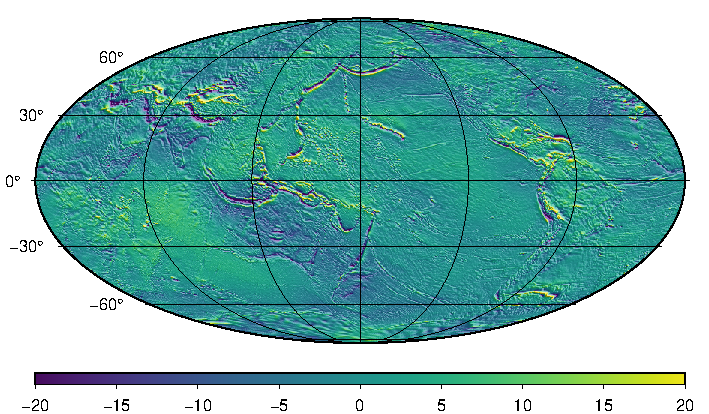
\includegraphics{./fig-deflections-xi.pdf}
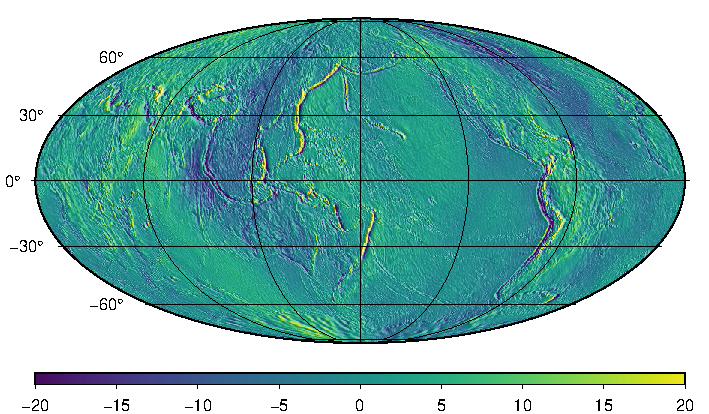
\includegraphics{./fig-deflections-eta.pdf}
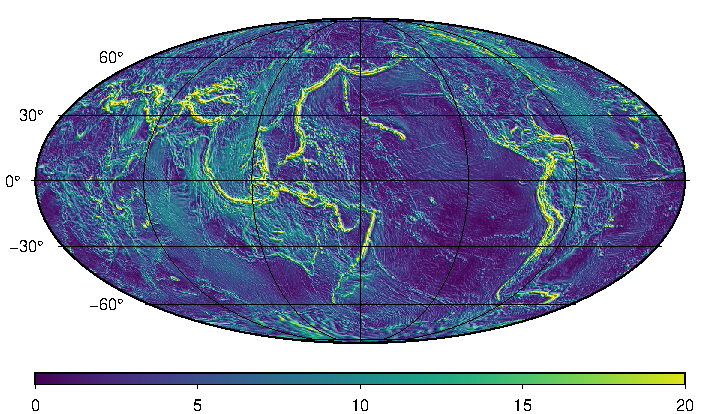
\includegraphics{./fig-deflections-theta.pdf}
\caption{Zložky zvislicovej odchýlky $\xi$ (vrchná mapa), $\eta$ (prostredná 
mapa) a celková zvislicová odchýlka~$\Theta$ (spodná mapa) pre zemské 
gravitačné pole vypočítané vzťahmi~(\ref{eq:deflection_total}) 
a~(\ref{eq:deflection_grav_s_sph}) zo sférického harmonického modelu EIGEN-6C4 
do stupňa~720 na povrchu elipsoidu~GRS80 (jednotky~$''$).  Normálne tiažové 
pole je generované ekvipotenciálnym elipsoidom~GRS80.}
\label{fig:deflections_ggm}
\end{figure}

Z~Obrázku~\ref{fig:deflections_ggm} vidíme, že zvislicové odchýlky dosahujú 
hodnoty zväčša na úrovni niekoľkých desiatok uhlových sekúnd a~len zriedkavo 
hodnoty väčšie ako uhlová minúta.  Najväčšie vychýlenie skutočnej tiažnice 
nastáva v~oblastiach, v~ktorých dochádza k~prudkej horizontálnej zmene 
poruchového potenciálu, napríklad v~oblastiach pohorí či tektonických zlomov.  
Toto pozorovanie možno vysvetliť horizontálnym deriváciami poruchového 
potenciálu vo vzťahoch~(\ref{eq:deflection_grav_s_sph}).  Vidíme tiež výraznú 
podobnosť medzi vrchnými dvoma mapami poruchy tiažového zrýchlenia na 
Obrázku~\ref{fig:dg_ggm_grs80} a zvislicovej odchýlky na 
Obrázku~\ref{fig:deflections_ggm}.  Táto podobnosť je daná úzkou súvislosťou 
medzi horizontálnymi zložkami vektorovej poruchy tiažového zrýchlenia 
a~zložkami zvislicovej odchýlky (pozri rovnice~\ref{eq:deflection_grav_s_sph}).






% -----------------------------------------------------------------------------

\chapter{Geoid}
\label{sec:geoid}

Vráťme sa na chvíľu do úvodnej kapitoly, v~ktorej sme načrtli dva prístupy 
k~definícii tvaru Zeme.  V~zmysle prvej definície je tvar Zeme daný jej 
skutočným fyzickým povrchom.  Určovaním takto chápaného tvaru Zeme a~jej 
vonkajšieho tiažového poľa sa zaoberá Molodenského teória 
\parencite{Molodensky1962,Borre_chapter8,MoritzAdvancedGeodesy,MoritzPhysicalGeodesy}.  
V~druhom prístupe je tvar Zeme definovaný geoidom, teda ekvipotenciálnou 
plochou.  Na týchto stranách sa budeme bližšie zaoberať iba druhým 
prístupom.\footnote{Pre Molodenského teóriu pozri 
napríklad~\textcite{Janak2006}.}

Z~Kapitol~\ref{sec:gravity_disturbance} až~\ref{sec:deflections} vieme, že 
medzi merateľné veličiny fyzikálnej geodézie patria najmä (no nielen) porucha 
tiažového zrýchlenia~$\delta g$, anomália tiažového zrýchlenia~$\Delta g$ 
a~zvislicové odchýlky~$\xi, \eta$.  Geoid preto určujeme spravidla z~týchto 
veličín.  Z~rovnice~(\ref{eq:N}) ďalej vieme, že na určenie výšky geoidu~$N$ 
nad referenčným elipsoidom (Obrázok~\ref{fig:geoid}) postačuje určiť poruchový 
potenciál na geoide~$T(P_0)$.\footnote{Normálne tiažové 
zrýchlenie~$\gamma(Q_0)$, ktoré vystupuje v~rovnici~(\ref{eq:N}), môžeme 
vypočítať jednoducho Somiglianovým vzťahom~(\ref{eq:somigliana}).}  
\emph{Linearizované} vzťahy medzi merateľnými veličinami fyzikálnej geodézie 
a~neznámym poruchovým potenciálom už poznáme (vzťahy~\ref{eq:dg_normals}, 
\ref{eq:Dg_fundamental_equation_geoid}, \ref{eq:Dg_fundamental_equation_earth}, 
\ref{eq:Dg_fundamental_equation_earth_sph}, 
\ref{eq:Dg_fundamental_equation_geoid_sph}, \ref{eq:deflection_grav_nat}, 
\ref{eq:deflection_grav_e}, \ref{eq:deflection_grav_s}).  Všimnime si však, že 
v~týchto rovniciach síce vystupuje poruchový potenciál, ktorý potrebujeme 
určiť, ale nachádza sa v~nich vo forme \emph{derivácie}, či už vertikálnej 
alebo horizontálnej.

Nech~$\DIFF_{\Delta g}$ a~$\DIFF_{\delta g}$ sú \emph{diferenciálne operátory}, 
ktoré transformujú poruchový potenciál na anomáliu a~poruchu tiažového 
zrýchlenia~$\Delta g$ a~$\delta g$.  Vo sférickej aproximácii majú tvar 
(rovnice~\ref{eq:Dg_fundamental_equation_geoid_sph} a~\ref{eq:dg_normals})
%
\begin{equation}
\label{eq:diff_Dg}
\begin{split}
\DIFF_{\Delta g} &= -\frac{\partial}{\partial r} - \frac{2}{r}{,}\\
%
\DIFF_{\delta g} &= -\frac{\partial}{\partial r}{.}
\end{split}
\end{equation}
%
Anomáliu a~poruchu tiažového zrýchlenia vo sférickej aproximácii potom môžeme 
zapísať nasledovne,
%
\begin{equation}
\label{eq:diff_operators}
\begin{split}
\Delta g &= \DIFF_{\Delta g}T{,}\\
%
\delta g &= \DIFF_{\delta g}T{.}
\end{split}
\end{equation}
%
Aby sme dokázali vypočítať poruchový potenciál, na ktorý 
v~rovniciach~(\ref{eq:diff_operators}) pôsobia diferenciálne operátory, 
potrebujeme nájsť \emph{integrálne operátory}~$\INT_{\Delta g}$ a~$\INT_{\delta 
g}$.  Tie následne aplikujeme na anomálie a~poruchy tiažového zrýchlenia na 
geoide, $\Delta g_0$ a~$\delta g_0$, čím získame hľadaný poruchový potenciál 
kdekoľvek na geoide alebo v~jeho vonkajšom priestore,
%
\begin{equation}
\label{eq:int_operators}
\begin{split}
T &= \INT_{\Delta g} \Delta g_0{,}\\
%
T &= \INT_{\delta g}\delta g_0{.}
\end{split}
\end{equation}

Integrálne vzťahy~(\ref{eq:int_operators}) budeme hľadať pomocou okrajových 
úloh pre poruchový potenciál.  S~pojmom okrajová úloha sme sa už čiastočne 
stretli v~Kapitole~\ref{sec:u_boundary_value_problem} a~nepriamo aj 
v~Kapitole~\ref{sec:meaning_of_laplace_equation_in_practice}.  
V~Kapitole~\ref{sec:boundary_value_problem} najprv načrtneme princíp určovania 
poruchového potenciálu pomocou okrajových úloh.  
V~Kapitolách~\ref{sec:stokes_integral} až~\ref{sec:poisson_integral} potom 
popíšeme rôzne typy okrajových úloh, s~ktorými sa vo fyzikálnej geodézii často 
stretávame.  Pri čítaní týchto kapitol si všimnime, že vonkajšie tiažové pole 
Zeme určujeme bez potreby priamej znalosti hustoty, podobne ako 
v~Kapitole~\ref{sec:spherical_harmonic_expansion}.  Okrajové úlohy budú totiž 
formulované tak, že informácia o~hustote Zeme bude zachytená vo vstupných 
anomáliách, resp. poruchách tiažového zrýchlenia 
(vzťahy~\ref{eq:int_operators}).  Tie v~praxi získavame gravimetrickým meraním 
veľkosti tiažového zrýchlenia (Kapitola~\ref{sec:gravity_measurements}), ktoré 
túto informáciu implicitne obsahuje (Kapitola~\ref{sec:gg}).  Pripomeňme, že na 
získanie poruchového potenciálu sa sústredíme preto, lebo výpočet výšky geoidu 
nad referenčným elipsoidom zo známeho poruchového potenciálu na geoide je 
jednoduchý (vzťah~\ref{eq:N}).

K~výpočtu geoidu zo zvislicových odchýlok pristúpime iným spôsobom.  Zatiaľ čo 
poruchy a~anomálie tiažového zrýchlenia možno chápať skôr fyzikálne, pretože 
priamo súvisia s~\emph{veľkosťou} tiažového zrýchlenia, zvislicové odchýlky 
možno vnímať geometricky (Obrázok~\ref{fig:deflections}), pretože sú spojené so 
\emph{smerom} tiažového zrýchlenia \parencite{MoritzPhysicalGeodesy}.  Na 
výpočet geoidu zo zvislicových odchýlok využijeme 
v~Kapitole~\ref{sec:geoid_astrogeodetic} práve geometrickú interpretáciu 
zvislicových odchýlok.

V~Kapitole~\ref{sec:other_geoid_determination_methods} spomenieme ďalšie metódy 
určovania geoidu a~na záver v~Kapitole~\ref{sec:vm_integral} pre úplnosť 
uvedieme spôsob výpočtu zvislicových odchýlok z~gravimetrických dát.


\section{Okrajová úloha pre poruchový potenciál}
\label{sec:boundary_value_problem}

Nech~$\Omega$ je vnútorná časť Zemského telesa ohraničená povrchom~$\partial 
\Omega$, v~tomto prípade geoidom (Obrázok~\ref{fig:boundary_value_problems}).  
O~hranici~$\partial \Omega$ budeme predpokladať, že je dostatočne 
hladká.\footnote{Pozri napríklad \textcite{SansoGeoidDetermination}.}  Táto 
podmienka je splnená, pretože geoid je ekvipoteciálna plocha (pozri vlastnosti 
ekvipotenciálnych plôch v~Kapitole~\ref{sec:equipotential_surface}).  Symbolom 
$\overline{\Omega} = \Omega \cup \partial\Omega$ budeme označovať zemské teleso 
spolu s~jeho povrchom.  Nech sa mimo telesa~$\overline{\Omega}$ nenachádzajú 
hmoty, teda napríklad ani nebeské telesá, ani zemská atmosféra či ani 
topografické hmoty.\footnote{Pre odstránenie gravitačného účinku topografických 
a~atmosférických hmôt pozri regularizáciu zemského telesa 
v~práci~\textcite{Janak2006}.}  Túto vonkajšiu oblasť označme~$\mathbb{R}^3 
- \overline{\Omega}$.

\begin{figure}[bt]
\centering
\input{./fig-boundary-value-problems.pdf_tex}
\caption{Geometrické znázornenie oblastí vystupujúcich v~okrajovej úlohe pre 
poruchový potenciál Zeme.}
\label{fig:boundary_value_problems}
\end{figure}

Našim cieľom je nájsť vzťahy, ktoré by umožnili získať poruchový potenciál na 
hranici~$\partial \Omega$ a v~celej oblasti~$\mathbb{R}^3 - \overline{\Omega}$ 
z~porúch alebo anomálií tiažového zrýchlenia, ktoré sú známe (odmerané) na 
hranici~$\partial \Omega$.  Nie je náročné uvedomiť si, že túto úlohu by nebolo 
možné vyriešiť bez toho, aby sme vedeli dostatočne veľa o~tom, ako sa poruchový 
potenciál \emph{mení} vo vonkajšom priestore hranice~$\partial\Omega$.  
Potrebnú informáciu o~zmene poruchového potenciálu v~priestore mimo Zeme 
zachytáva Laplaceova rovnica~(\ref{eq:laplace_xyz_t}).\footnote{Pre diskusiu 
o~význame Laplaceovej rovnice pre fyzikálnu geodéziu pozri 
Kapitolu~\ref{sec:meaning_of_laplace_equation_in_practice}.}  \emph{Okrajovou 
úlohou pre poruchový potenciál} teda rozumieme hľadanie takého riešenia 
diferenciálnej rovnice~(\ref{eq:laplace_xyz_t}), ktoré v~oblasti~$\mathbb{R}^3 
- \overline\Omega$ vyhovuje rovnici~(\ref{eq:laplace_xyz_t}) a~na 
hranici~$\partial \Omega$ reprodukuje zadanú podmienku.  Podmienku zadanú na 
hranici~$\partial \Omega$ nazývame \emph{okrajová podmienka}.  Okrajová 
podmienka musí byť v~nejakom vzťahu voči hľadanému poruchovému potenciálu.  
Okrajová podmienka tak môže byť zadaná napríklad pomocou niektorej 
z~nasledovných veličín:
%
\begin{itemize}
\item lineárna kombinácia poruchového potenciálu~$T$ a~jeho prvej derivácie 
v~smere vonkajšej normály v~podobe anomálie tiažového zrýchlenia~$\DIFF_{\Delta 
g}T$ (rovnica~\ref{eq:Dg_fundamental_equation_geoid_sph}) (táto okrajová 
podmienka sa zvykne nazývať \emph{Newtonova okrajová podmienka}; 
Kapitola~\ref{sec:stokes_integral}),
%
\item prvá derivácia poruchového potenciálu v~smere vonkajšej normály v~podobe 
poruchy tiažového zrýchlenia~$\DIFF_{\delta g} T$ (rovnica~\ref{eq:dg_normals}) 
(\emph{Neumannova okrajová podmienka}; Kapitola~\ref{sec:hotine_integral}),
%
\item samotný poruchový potenciál~$T$ (\emph{Dirichletova okrajová podmienka}; 
Kapitola~\ref{sec:poisson_integral}),
%
\item druhá vertikálna derivácia poruchového potenciálu~$\partial^2 
T / \partial r^2$ (táto okrajová úloha nie je predmetom tejto práce), atď.
\end{itemize}
%
V~praxi závisí voľba okrajovej podmienky najmä od typu dostupných dát.

Vzťahy~(\ref{eq:int_operators}) označujú všeobecný zápis riešenia získaného 
z~prvých dvoch uvedených okrajových úloh.  Na pravej strane týchto rovníc 
vystupujú okrajové podmienky na hranici~$\partial \Omega$ (odmerané vstupné 
dáta~$\Delta g_0$ alebo~$\delta g_0$ na geoide) a~na ľavej strane vystupuje 
hľadaný poruchový potenciál~$T$, ktorý možno vypočítať nielen na 
hranici~$\partial\Omega$ ale aj v~oblasti~$\mathbb{R}^3 - \overline\Omega$.  
Spomeňme, že poruchový potenciál získaný z~každej z~týchto okrajových úloh je 
totožný, teda napríklad
%
\begin{equation}
T = \INT_{\Delta g} \Delta g_0 = \INT_{\delta g}\delta g_0{.}
\end{equation}
%
Rozdielne sú iba okrajové podmienky, a~teda následne aj integrálne 
operátory~$\INT_{\Delta g}$ a~$\INT_{\delta g}$.


\subsubsection{Poznámka k~okrajovým a~počiatočným úlohám}

V~matematike je \emph{okrajová úloha} všeobecný pojem, ktorý označuje riešenie 
diferenciálnej rovnice so zadanou okrajovou podmienkou.  Okrajová podmienka sa 
spravidla vzťahuje k~priestoru (napríklad povrch telesa) a~diferenciálna 
rovnica je riešená v~priestore.  Naproti tomu, pojmom \emph{počiatočná úloha} 
označujeme riešenie diferenciálnej rovnice so zadanou počiatočnou podmienkou.  
Počiatočná podmienka sa zvyčajne vzťahuje k~časovému okamihu.  Počiatočné úlohy 
sa teda zaoberajú vývojom diferenciálnej rovnice v~čase.  Podrobnejšie 
informácie o~okrajových a~počiatočných úlohách, o~ich klasifikácii a~o~metódach 
ich riešenia je možné nájsť napríklad v~prácach \textcite{Janak2006} 
a~\textcite{Macak2021}.



\section{Stokesov integrál}
\label{sec:stokes_integral}

Definujme okrajovú úlohu pre poruchový potenciál s~využitím okrajovej podmienky 
vo forme sférickej aproximácie anomálie tiažového zrýchlenia:
%
\begin{alignat}{2}
\nabla^2 T(P) &= 0{,} &&P \in \mathbb{R}^3 
- \overline\Omega{,}\label{eq:bvp_Dg_laplace}\\
\Delta g(P) &= -\left.\frac{\partial T}{\partial r}\right|_P 
- \left.\frac{2}{r}\right|_P \, T(P){,} \quad &&P \in 
\partial\Omega{,}\label{eq:bvp_Dg_boundary_condition}\\
T(P) &\rightarrow 0 &&\textrm{pre} \quad P \rightarrow 
\infty{.}\label{eq:bvp_Dg_t_infty}
\end{alignat}
%
Vzťah~(\ref{eq:bvp_Dg_laplace}) definuje diferenciálnu rovnicu, ktorá je 
predmetom riešenia okrajovej úlohy na oblasti~$\mathbb{R}^3 - \overline\Omega$.  
Rovnica~(\ref{eq:bvp_Dg_boundary_condition}) špecifikuje konkrétny typ 
okrajovej podmienky, ktorá platí na geoide~$\partial\Omega$.  
Vzťah~(\ref{eq:bvp_Dg_t_infty}) dodáva ďalšiu informáciu o~poruchovom 
potenciáli; hovorí, že s~narastajúcou vzdialenosťou bodu~$P$ od 
Zeme~$\overline\Omega$ sa poruchový potenciál~$T$ blíži k~nule (pozri 
vzťah~\ref{eq:t_infty}).  Bez~rovníc~(\ref{eq:bvp_Dg_boundary_condition}) 
a~(\ref{eq:bvp_Dg_t_infty}) by mala diferenciálna 
rovnica~(\ref{eq:bvp_Dg_laplace}) nekonečne veľa riešení.  
Rovnice~(\ref{eq:bvp_Dg_boundary_condition}) a~(\ref{eq:bvp_Dg_t_infty}) tak 
zabezpečujú, že získame práve jedno riešenie rovnice~(\ref{eq:bvp_Dg_laplace}).  
Odvodenie riešenia okrajovej úlohy v~tejto práci vynecháme a~zameriame sa skôr 
na popis získanej rovnice.  Odvodenie je možné nájsť napríklad 
v~prácach~\textcite{MoritzPhysicalGeodesy} a~\textcite{Janak2006}.

Riešením okrajovej úlohy~(\ref{eq:bvp_Dg_laplace}) až~(\ref{eq:bvp_Dg_t_infty}) 
je vzťah
%
\begin{equation}
\label{eq:stokes}
T(P) = \frac{R}{4\pi} \, \iint\limits_{\sigma} S(P, P') \, \Delta g(P') \, 
\diff \sigma(P'){,} \quad P \in \left( \mathbb{R}^3 - \overline\Omega \right) 
\cup \partial\Omega{,} \quad P' \in \partial\Omega{,}
\end{equation}
%
ktorý sa nazýva \emph{Stokesov integrál}.  Symbol~$P(r, \varphi, \lambda)$ 
označuje bod, v~ktorom je počítaný poruchový potenciál 
(Obrázok~\ref{fig:surface_integral}), $P'(R, \varphi', \lambda')$ je bod na 
geoide, $R$~označuje polomer referenčnej sféry (napríklad stredný či rovníkový 
polomer Zeme), $\sigma$ je jednotková sféra, $\diff\sigma(P')$ je jej 
diferenciál v~bode~$P'$,
%
\begin{equation}
\label{eq:diff_sigma}
\diff\sigma(P') = \cos\varphi' \, \diff\varphi' \, \diff\lambda'{,}
\end{equation}
%
a~$S$ je \emph{Stokesovo integračné jadro} (niekedy tiež nazývané 
\emph{Stokesova funkcia}).  Stokesovo jadro~$S$ závisí iba od vzájomnej polohy 
bodov~$P$ a~$P'$ \parencite{MoritzPhysicalGeodesy},
%
\begin{equation}
\label{eq:stokes_kernel_general}
\begin{split}
S(P, P') &= S(r, \psi)\\
%
&= \frac{2R}{\ell} + \frac{R}{r} - 3\frac{R \, \ell}{r^2} - \frac{R^2}{r^2} \, 
\cos\psi\left( 5 + 3 \, \ln \frac{r - R \, \cos\psi + \ell}{2 \, r} \right){,}
\end{split}
\end{equation}
%
kde~$\ell$ a~$\psi$ sú Euklidovská a~sférická vzdialenosť medzi bodmi~$P$ 
a~$P'$ (rovnice~\ref{eq:l_sph} a~\ref{eq:cospsi}).

\begin{figure}[bt]
\centering
\input{./fig-surface-integral.pdf_tex}
\caption{Výpočtový bod~$P(\varphi, \lambda)$ premietnutý na jednotkovú sféru 
a~diferenciálny integračný element~$\diff\sigma = \diff\sigma(P')$ na 
jednotkovej sfére.  Symbol~$\psi$ označuje sférickú vzdialenosť medzi~$P$ 
a~$\diff\sigma$ a~$\alpha$ označuje azimut spojnice~$P$ a~$\diff\sigma$.}
\label{fig:surface_integral}
\end{figure}

Stokesov integrál~(\ref{eq:stokes}) umožňuje vypočítať poruchový potenciál 
kdekoľvek v~oblasti~$\left( \mathbb{R}^3 - \overline\Omega\right) \cup 
\partial\Omega$.  Osobitne zaujímavý je prípad, v~ktorom výpočtový bod leží na 
rovnakej sfére ako anomálie tiažového zrýchlenia, teda keď~$r = R$.  Všeobecný 
tvar Stokesovho jadra~(\ref{eq:stokes_kernel_general}) potom prejde do tvaru, 
ktorý závisí iba od sférickej vzdialenosti~$\psi$ 
\parencite{MoritzPhysicalGeodesy},
%
\begin{equation}
\label{eq:stokes_kernel}
\begin{split}
S(\psi) = \frac{1}{\sin\dfrac{\psi}{2}} - 6 \, \sin\frac{\psi}{2} + 1 - 5 \, 
\cos\psi - 3 \, \cos\psi \, \ln\left( \sin\frac{\psi}{2} + \sin^2\frac{\psi}{2} 
\right){.}
\end{split}
\end{equation}
%
Stokesov integrál sa v~takom prípade zvykne zapisovať v~zjednodušenej forme
%
\begin{equation}
\label{eq:stokes_simplified}
T = \frac{R}{4\pi} \, \iint\limits_{\sigma} S(\psi) \, \Delta g_0 \, \diff 
\sigma{,}
\end{equation}
%
pričom~$T = T(P)$, $P(R, \varphi, \lambda) \in \partial\Omega$, $\Delta g_0 
= \Delta g_0(P')$, $P'(R, \varphi', \lambda') \in \partial\Omega$ 
a~$\diff\sigma = \diff\sigma(P')$.  Symbol~$\Delta g_0$ označuje anomálie 
tiažového zrýchlenia na geoide (pozri Kapitolu~\ref{sec:gravity_anomaly}).

Dosadením rovnice~(\ref{eq:stokes_simplified}) do Brunsovho vzorca~(\ref{eq:N}) 
získame vzťah na výpočet výšky geoidu nad referenčným elipsoidom z~anomálií 
tiažového zrýchlenia na geoide, teda v~širšom zmysle z~meraného tiažového 
zrýchlenia,
%
\begin{equation}
\label{eq:stokes_N}
N = \frac{R}{4\pi \, \gamma_0} \, \iint\limits_{\sigma} S(\psi) \, \Delta g_0 
\, \diff \sigma{,}
\end{equation}
%
kde $\gamma_0 = \gamma(Q_0)$.  Rovnica~(\ref{eq:stokes_N}) predstavuje jednu zo 
základných rovníc fyzikálnej geodézie.

Dodajme, že zo vzťahu~(\ref{eq:stokes}) vyplýva tvar hľadaného integrálneho 
operátora~$\mathcal{I}_{\Delta g}$ z~rovnice~(\ref{eq:int_operators}),
%
\begin{equation}
\label{eq:iDg}
\mathcal{I}_{\Delta g}( \, \cdot \, )(P) = \frac{R}{4\pi} \, 
\iint\limits_\sigma S(P, P') ( \, \cdot \, )(P') \, \diff\sigma(P'){,}
\end{equation}
%
kde symbol $(\, \cdot \,)$ označuje funkciu, na ktorú je integrálny operátor 
aplikovaný.


\subsection{Stokesovo integračné jadro}
\label{sec:stokes_kernel}

Význam Stokesovej funkcie vo vzťahu~(\ref{eq:stokes_simplified}) lepšie 
pochopíme z~grafického znázornenia jej priebehu 
(Obrázok~\ref{fig:stokes_kernel}).  Z~obrázku 
a~z~rovnice~(\ref{eq:stokes_kernel}) je zrejmé, že hodnota Stokesovej funkcie 
klesá so zväčšujúcou sa sférickou vzdialenosťou~$\psi$ až po vzdialenosť~$\psi 
\approx 72^\circ$, po ktorej začína mierne stúpať s~narastajúcim~$\psi$.  
V~súvislosti s~rovnicou~(\ref{eq:stokes_simplified}) to znamená, že na hodnotu 
poruchového potenciálu~$T(P)$ majú najväčší vplyv anomálie tiažového 
zrýchlenia~$\Delta g(P')$, ktoré sa nachádzajú v~blízkosti výpočtového 
bodu~$P$.  Inými slovami, anomálie tiažového zrýchlenia~$\Delta g(P')$ 
v~blízkom okolí výpočtového bodu sú v~rovnici~(\ref{eq:stokes_simplified}) 
násobené (\emph{vážené}) väčšími hodnotami Stokesovej funkcie~$S$ ako tie 
anomálie, ktoré sa nachádzajú ďaleko od výpočtového bodu; ich relatívny prínos 
do hodnoty poruchového potenciálu je tak väčší ako v~prípade veľkých 
vzdialeností medzi~$P$ a~$\diff\sigma$.  Na Obrázku~\ref{fig:stokes_kernel} 
tiež vidíme, že Stokesovo integračné jadro nadobúda nulové hodnoty pre sférické 
vzdialenosti približne~$39^\circ$ a~$117^\circ$ \parencite{TorgeGeodesy}.  
Príspevok anomálií tiažového zrýchlenia, ktoré sa nachádzajú v~týchto 
vzdialenostiach voči výpočtovému bodu, je preto nulový.

\begin{figure}[bt]
\centering
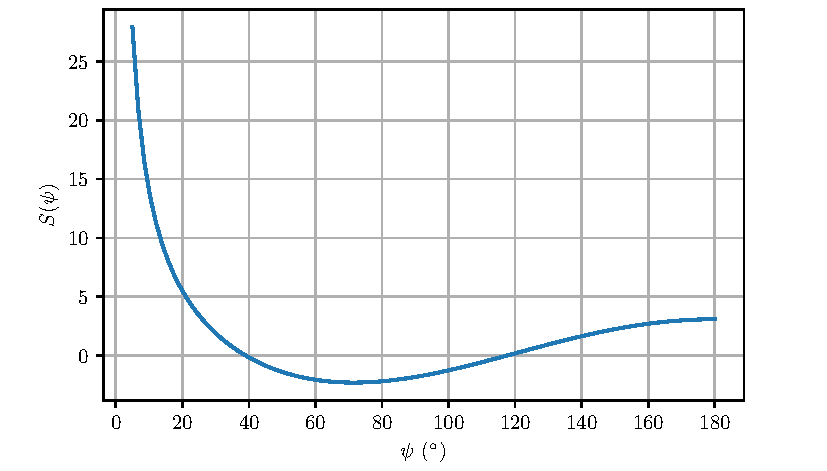
\includegraphics{./fig-stokes-kernel.pdf}
\caption{Stokesova funkcia~$S(\psi)$ (vzťah~\ref{eq:stokes_kernel}) na 
intervale~$[5^\circ, 180^\circ]$.}
\label{fig:stokes_kernel}
\end{figure}

Stokesova funkcia má niekoľko ďalších zaujímavých vlastností.
%
\begin{itemize}
\item \emph{Singularita}.  Pre~$P(r, \varphi, \lambda) \rightarrow P'(R, 
\varphi', \lambda')$ sa hodnota Stokesovej 
funkcie~(\ref{eq:stokes_kernel_general}) blíži k~nekonečnu (pre pojem 
singularita pozri tiež Kapitolu~\ref{sec:spheroidal_harmonics}),
%
\begin{equation}
\label{eq:stokes_singularity}
\lim\limits_{P \rightarrow P'} S(P, P') = \infty{.}
\end{equation}
%
K~singularite Stokesovej funkcie dochádza vtedy, keď integrál~(\ref{eq:stokes}) 
je počítaný na tej sfére, na ktorej je zadaná okrajová podmienka v~podobe 
anomálií tiažového zrýchlenia, teda keď~$r = R$, a~súčasne keď~$(\varphi, 
\lambda) = (\varphi', \lambda')$.  Napriek singularite Stokesovho integračného 
jadra však bude výsledok integrácie~(\ref{eq:stokes}), teda poruchový potenciál 
v~bode~$P$, nadobúdať \emph{konečnú} hodnotu (pre podobnú situáciu v~súvislosti 
s~Newtonovým integrálom pozri tiež diskusiu zo záveru 
Kapitoly~\ref{sec:potential_theory}).  V~numerických výpočtoch je ale i~tak 
potrebné venovať singularite osobitnú pozornosť a~použiť vhodné matematické 
úpravy Stokesovho integrálu (pozri napríklad \cite{MoritzPhysicalGeodesy} či 
\cite{Hees1991}).  Dodajme, že vo všeobecnosti neplatí, že každé singulárne 
integračné jadro vedie ku konečným hodnotám integrálu.  To, či je hodnota 
integrálu konečná alebo nie, závisí od typu singularity.
%
\item \emph{Homogénnosť}.  Hodnota Stokesovho integračného jadra nezávisí od 
polohy bodov~$P$ a~$P'$ v~priestore za predpokladu, že $r$ a~$\psi$ ostávajú 
nezmenené.  Ak sa napríklad body~$P$ a~$P'$ nachádzajú na tej istej sfére a~na 
tom istom meridiáne, hodnota Stokesovej funkcie~(\ref{eq:stokes_kernel}) je 
rovnaká bez ohľadu na to, v~ktorej časti meridiánu a~na ktorom meridiáne sa 
body~$P$ a~$P'$ nachádzajú, pokiaľ ich vzdialenosť~$\psi$ ostáva nezmenená.
%
\item \emph{Izotropnosť}.  Hodnota Stokesovho integračného jadra nezávisí od 
azimutu~$\alpha$ spojnice bodov~$P$ a~$P'$ (pozri 
Obrázok~\ref{fig:surface_integral}).
\end{itemize}

Stokesovu funkciu je možné ekvivalentne vyjadriť aj rozvojom do radu 
Legendreových polynómov \parencite{MoritzPhysicalGeodesy},
%
\begin{equation}
\label{eq:stokes_spectral}
S(r, \psi) = \sum_{n = 2}^{\infty} \frac{2n + 1}{n - 1} \, \left( \frac{R}{r} 
\right)^{n + 1} \, P_n(\cos\psi){.}
\end{equation}
%
Ide pritom o~rozvoj typu~(\ref{eq:f_synthesis}).  
Rovnice~(\ref{eq:stokes_kernel_general}) a~(\ref{eq:stokes_kernel}) nazývame 
\emph{priestorový tvar} Stokesovho integračného jadra.  
Vzťah~(\ref{eq:stokes_spectral}) nazývame \emph{spektrálny tvar} Stokesovho 
integračného jadra.  To, ktorý tvar je výhodnejšie použiť, často závisí od 
aplikácie.  Ak anomálie tiažového zrýchlenia~$\Delta g$ nachádzajúce sa 
v~integráli~(\ref{eq:stokes}) boli získané meraním, môže byť vhodnejšie použiť 
priestorový tvar.  Je to preto, lebo odmerané gravitačné, resp. tiažové 
zrýchlenie zahŕňa vplyv všetkých harmonických stupňov (pozri nekonečné sumácie 
vo vzťahoch~\ref{eq:vgx_sh}, \ref{eq:vgy_sh} a~\ref{eq:vgz_sh}), rovnako tak 
ako priestorový tvar Stokesovho jadra~(\ref{eq:stokes_kernel_general}) 
implicitne obsahuje všetky harmonické stupne zo spektrálneho 
tvaru~(\ref{eq:stokes_spectral}) (pravá strana 
rovnice~\ref{eq:stokes_kernel_general} sa rovná pravej strane 
rovnice~\ref{eq:stokes_spectral}).  Výpočet Stokesovho jadra spektrálnym tvarom 
by bol v~tejto situácii nevhodný, pretože nekonečný rad by musel byť 
v~praktickom výpočte obmedzený na konečný počet členov, čo by spôsobilo 
aproximačné chyby.  Ak ale boli anomálie tiažového zrýchlenia~$\Delta g$ 
vypočítané z~konečného sférického harmonického radu vzťahom~(\ref{eq:Dg_sh_sa}) 
do stupňa~$N$, potom môže byť výhodnejšie použiť spektrálny 
tvar~(\ref{eq:stokes_spectral}) rozvinutý do identického maximálneho 
stupňa~$N$.\footnote{Z~teoretického hľadiska môže byť ekvivalentne použitý aj 
priestorový tvar Stokesovho jadra, prípadne spektrálny tvar rozvinutý do 
vyššieho stupňa ako~$N$ \parencite[pozri napríklad][]{Freeden2009}.}

Všimnime si, že vo vzťahoch~(\ref{eq:stokes_kernel_general}), 
(\ref{eq:stokes_kernel}) a~(\ref{eq:stokes_spectral}) sa \emph{nenachádza} 
vplyv nultého harmonického stupňa (sumácia v~rovnici~\ref{eq:stokes_spectral} 
začína od stupňa~$2$ a~pravé strany týchto rovníc sú si rovné).  S~uvážením 
nultého harmonického stupňa nadobudne Stokesovo integračné jadro nasledovné 
tvary,
%
\begin{align}
S(r, \psi) &= \frac{2R}{\ell} - 3\frac{R \, \ell}{r^2} - \frac{R^2}{r^2} \, 
\cos\psi\left( 5 + 3 \, \ln \frac{r - R \, \cos\psi + \ell}{2 \, r} \right){,}
\label{eq:stokes_kernel_general_n0}
\\
%
S(\psi) &= \frac{1}{\sin\dfrac{\psi}{2}} - 6 \, \sin\frac{\psi}{2} - 5 \, 
\cos\psi - 3 \, \cos\psi \, \ln\left( \sin\frac{\psi}{2} + \sin^2\frac{\psi}{2} 
\right){,}
\label{eq:stokes_kernel_n0}
\\
%
S(r, \psi) &= \sum_{n = 0{,}\, n \neq 1}^{\infty} \frac{2n + 1}{n - 1} \, 
\left( \frac{R}{r} \right)^{n + 1} \, P_n(\cos\psi){.}
\label{eq:stokes_spectral_n0}
\end{align}
%
Tieto rovnice je potrebné použiť vtedy, keď anomálie tiažového zrýchlenia vo 
vzťahu~(\ref{eq:stokes}) obsahujú aj vplyv nultého harmonického člena 
z~rovnice~(\ref{eq:Dg_sh_sa}).  Všimnime si tiež, že stupeň~$n$ 
v~rovnici~(\ref{eq:stokes_spectral_n0}) nesmie byť rovný~$1$ (aby bolo 
zamedzené deleniu nulou), čo je v~súlade so skutočnosťou, že harmonický 
stupeň~$n = 1$ nevplýva na anomálie tiažového zrýchlenia (pozri poznámku 
k~rovnici~\ref{eq:Dg_sh_sa}).


\subsection{Stokesov integrál ako konvolučný integrál}
\label{sec:stokes_convolution}

Výpočtom integrálu~(\ref{eq:stokes}) získame poruchový potenciál v~bode~$P$, 
teda jedno číslo.  Ak chceme získať poruchový potenciál v~ďalšom bode~$P_1$, 
integráciu je potrebné zopakovať s~novým výpočtovým bodom~$P_1$.  Dôvod je ten, 
že hoci anomálie tiažového zrýchlenia~$\Delta g(P')$ sú identické (daná funkcia 
na hranici~$\partial\Omega$), zmena polohy výpočtového bodu z~$P$ na~$P_1$ 
spôsobí, že nové Stokesovo integračné jadro~$S(P_1, P')$ bude vážiť tie isté 
anomálie tiažového zrýchlenia~$\Delta g(P')$ iným spôsobom ako predošlé 
integračné jadro~$S(P, P')$.  Ak teda chceme získať poruchový potenciál~$P$ 
v~každom bode na Zemi, výpočtový bod~$P$ je potrebné vnímať ako premennú 
a~integráciu opakovať vo všetkých bodoch na sfére.  Výsledkom bude nová 
funkcia, ktorou je poruchový potenciál na celej sfére.  Transformovali sme teda 
dve funkcie, Stokesovo integračné jadro~$S$ a~anomálie tiažového 
zrýchlenia~$\Delta g$, na tretiu funkciu, poruchový potenciál~$T$.  Tento 
proces sa nazýva \emph{konvolúcia} a~symbolicky ho zapisujeme nasledovne,
%
\begin{equation}
\label{eq:stokes_convolution}
\frac{R}{4 \, \pi}(S * \Delta g)(P) = \frac{R}{4\pi} \, \iint\limits_\sigma 
S(P, P') \, \Delta g(P') \, \diff\sigma(P'){,}
\end{equation}
%
kde symbol~$*$ označuje konvolučné násobenie funkcií~$S$ a~$\Delta g$.

Vo fyzikálnej geodézii sa stretávame s~konvolučnými integrálmi veľmi často 
(pozri napríklad \cite{Jekeli2017}).  Konvolučným integrálom je napríklad aj 
Newtonov integrál~(\ref{eq:vg_body}).  Vo vzťahu~(\ref{eq:vg_body}) hrajú 
hustota~$\rho$ a~prevrátená hodnota vzdialenosti~$1 \slash \ell$ podobnú úlohu 
akú majú anomálie tiažového zrýchlenia~$\Delta g$ a~Stokesovo jadro~$S$ vo 
vzťahu~(\ref{eq:stokes}). Konvolučnými integrálmi sú tiež~integrály, ktoré sú 
odvodené z~Newtonovho integrálu.  Všimnime si napríklad, že vo 
vzťahu~(\ref{eq:gg_body}), ktorý je odvodený z~Newtonovho integrálu, vystupuje 
tá istá hustota ako v~rovnici~(\ref{eq:vg_body}).  Keďže ale vzťah medzi 
gravitačným zrýchlením a~hustotou je iný ako vzťah medzi gravitačným 
potenciálom a~hustotou, konvolučné jadro~$\vec r \slash \ell^3$ 
v~rovnici~(\ref{eq:gg_body}) je iné ako v~rovnici~(\ref{eq:vg_body}).  Rozličné 
integračné jadrá teda transformujú tú istú funkciu rozdielne.

Konvolučné integrály sa vyskytujú aj v~mnohých oblastiach matematiky, fyziky 
a~v~ďalších vedných disciplínach.  Jednou z~praktických aplikácií konvolúcie je 
potlačenie šumu na zvukových nahrávkach.  Vstupný signál, teda pôvodná 
nahrávka, je konvolučne vynásobený vhodným integračným jadrom, výsledkom čoho 
je upravená nahrávka s~potlačeným šumom, teda výstupný signál.  Aplikáciou 
iného konvolučného jadra na tú istú nahrávku môžeme zvýrazniť inú časť spektra 
na nahrávke, povedzme nízke frekvencie a~pod.  Pre konvolučné integrály je 
typické, že ich numerický výpočet je časovo veľmi náročný.  Snahou preto je 
použiť efektívne algoritmy, napríklad rýchlu Fourierovu transformáciu 
\parencite{PressNumericalRecipes} či vlnkovú transformáciu 
\parencite{KellerWavelets}.  Obe transformácie sa používajú aj na efektívny 
výpočet konvolučných integrálov fyzikálnej geodézie \parencite[pozri 
napríklad][]{Forsberg1984,Freeden1998a,SansoGeoidDetermination}.


\subsection{Sférická aproximácia v~Stokesovom integráli}
\label{sec:stokes_spherical_approximation}

Riešenie~(\ref{eq:stokes}) okrajovej úlohy~(\ref{eq:bvp_Dg_laplace}) 
až~(\ref{eq:bvp_Dg_t_infty}) bolo získané s~využitím sférickej aproximácie.  
Sférická aproximácia bola použitá jednak v~definícii okrajovej 
podmienky~(\ref{eq:bvp_Dg_boundary_condition}), ale tiež v~riešení okrajovej 
úlohy, čo má niekoľko dôsledkov pre praktické určovanie geoidu 
vzťahom~(\ref{eq:stokes_N}).  Hoci získané riešenie~(\ref{eq:stokes}) využíva 
anomálie tiažového zrýchlenia na geoide~$\Delta g_0$, samotná integrácia sa 
nevykonáva na geoide, ktorý má komplikovaný tvar, ale na sfére s~polomerom~$R$, 
ktorá geoid aproximuje.  Neznamená to však, že výšky geoidu získané 
vzťahom~(\ref{eq:stokes_N}) sú vztiahnuté k~referenčnej sfére s~polomerom~$R$.  
Naopak, vzťahujú sa k~použitému ekvipotenciálnemu elipsoidu, preto aj normálne 
tiažové zrýchlenie~$\gamma_0$ v~rovnici~(\ref{eq:stokes_N}) má byť počítané 
Somiglianovým vzťahom pre ekvipotenciálny elipsoid 
(rovnica~\ref{eq:somigliana}).

Sférická aproximácia spôsobuje relatívnu chybu v~určení geoidu na úrovni~$0.003 
\, N$, teda dosahuje hodnoty menšie ako 1~m \parencite{MoritzPhysicalGeodesy}.  
Pre spresnenie riešenia je potrebné zaviesť korekciu zo sploštenia referenčného 
elipsoidu \parencite{Claessens2006}, prípadne integrovať priamo na 
ekvipotenciálnom elipsoide \parencite{Martinec1997}.


\section{Hotineov integrál}
\label{sec:hotine_integral}

Definujme teraz takú okrajovú úlohu, ktorá umožní vypočítať poruchový potenciál 
z~porúch tiažového zrýchlenia vo sférickej aproximácii:
%
\begin{alignat}{2}
\nabla^2 T(P) &= 0{,} &&P \in \mathbb{R}^3 
- \overline\Omega{,}\label{eq:bvp_dg_laplace}\\
\delta g(P) &= -\left.\frac{\partial T}{\partial r}\right|_P{,} \quad &&P \in 
\partial\Omega{,}\label{eq:bvp_dg_boundary_condition}\\
T(P) &\rightarrow 0 &&\textrm{pre} \quad P \rightarrow 
\infty{.}\label{eq:bvp_dg_t_infty}
\end{alignat}

Riešením okrajovej úlohy~(\ref{eq:bvp_dg_laplace}) až~(\ref{eq:bvp_dg_t_infty}) 
je rovnica (pre odvodenie pozri napríklad \cite{MoritzPhysicalGeodesy} alebo 
\cite{SansoGeoidDetermination})
%
\begin{equation}
\label{eq:hotine}
T(P) = \frac{R}{4\pi} \, \iint\limits_{\sigma} H(P, P') \, \delta g(P') \, 
\diff \sigma(P'){,} \quad P \in \left( \mathbb{R}^3 - \overline\Omega \right) 
\cup \partial\Omega{,} \quad P' \in \partial\Omega{.}
\end{equation}
%
Vzťah~(\ref{eq:hotine}) sa nazýva \emph{Hotineov integrál} a~funkcia~$H$ sa 
nazýva \emph{Hotineovo integračné jadro}.  Všeobecný tvar Hotineovho jadra je 
daný vzťahom \parencite{SansoGeoidDetermination}
%
\begin{equation}
\label{eq:hotine_kernel_general}
H(P, P') = H(r, \psi) = \frac{2R}{\ell} - \ln\left(\frac{\ell + R - r \, 
\cos\psi}{r \, (1 - \cos\psi)}\right){.}
\end{equation}
%
Pre~$r = R$ sa Hotineovo jadro zjednoduší do tvaru 
(Obrázok~\ref{fig:hotine_kernel})
%
\begin{equation}
\label{eq:hotine_kernel}
H(\psi) = \frac{1}{\sin\dfrac{\psi}{2}} - \ln\left( 
1 + \frac{1}{\sin\dfrac{\psi}{2}} \right){.}
\end{equation}
%
Spektrálna reprezentácia Hotineovho jadra je daná vzťahom
%
\begin{equation}
\label{eq:hotine_spectral}
H(r, \psi) = \sum_{n = 0}^{\infty} \frac{2n + 1}{n + 1} \, \left( \frac{R}{r} 
\right)^{n + 1} \, P_n(\cos\psi){.}
\end{equation}
%
Podobne ako Stokesov integrál, aj Hotineov integrál~(\ref{eq:hotine}) patrí 
medzi konvolučné integrály (Kapitola~\ref{sec:stokes_convolution}) a~bol 
získaný vo sférickej aproximácii 
(Kapitola~\ref{sec:stokes_spherical_approximation}).  Hľadaný tvar integrálneho 
operátora~$\mathcal{I}_{\delta g}$ z~rovnice~(\ref{eq:int_operators}) je zrejmý 
z~porovnania rovníc~(\ref{eq:stokes}), (\ref{eq:iDg}) a~(\ref{eq:hotine}).

\begin{figure}[bt]
\centering
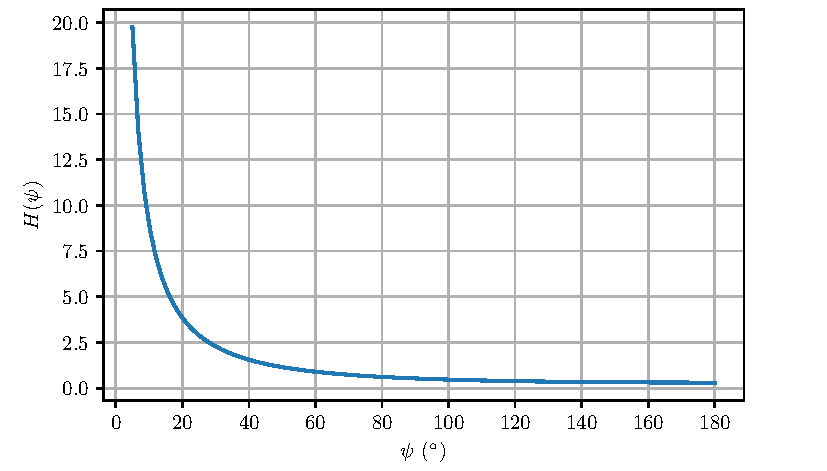
\includegraphics{./fig-hotine-kernel.pdf}
\caption{Hotineova funkcia~$H(\psi)$ (vzťah~\ref{eq:hotine_kernel}) na 
intervale~$[5^\circ, 180^\circ]$.}
\label{fig:hotine_kernel}
\end{figure}

Hotineovo integračné jadro má podobné vlastnosti ako Stokesovo integračné jadro 
(Kapitola~\ref{sec:stokes_kernel}), teda je singulárne, homogénne a izotropné.  
Na rozdiel od Stokesovho jadra ide o~monotónne klesajúcu funkciu 
(Obrázok~\ref{fig:hotine_kernel}), teda čím ďalej sa nachádza integračný 
element $\diff\sigma$ od výpočtového bodu~$P$, tým menšia váha~$H$ je 
v~Hotineovom integráli~(\ref{eq:hotine}) pridelená príslušnej poruche tiažového 
zrýchlenia.

Dosadením vzťahu~(\ref{eq:hotine}) pre~$P \in \partial\Omega$ do Brunsovho 
vzorca~(\ref{eq:N}) získame vzťah na výpočet geoidu z~porúch tiažového 
zrýchlenia,
%
\begin{equation}
\label{eq:hotine_N}
N = \frac{R}{4\pi \, \gamma_0} \, \iint\limits_{\sigma} H(\psi) \, \delta g_0 
\, \diff \sigma{,}
\end{equation}
%
kde symbol~$\delta g_0$ označuje poruchy tiažového zrýchlenia na geoide.  
Vzťah~(\ref{eq:hotine_N}) možno bezpochyby zaradiť medzi najdôležitejšie vzťahy 
fyzikálnej geodézie.

M.~Hotine (1898~-- 1968) bol anglický geodet.  Jeho kniha \textit{Matematická 
geodézia} z~roku 1969 patrí medzi fundamentálne geodetické práce.

\section{Poissonov integrál}
\label{sec:poisson_integral}

Posledná geodetická okrajová úloha, ktorú v~tejto práci spomenieme, je okrajová 
úloha pre poruchový potenciál so zadanou okrajovou podmienkou vo forme 
poruchového potenciálu:
%
\begin{alignat}{2}
\nabla^2 T(P) &= 0{,} &&P \in \mathbb{R}^3 
- \overline\Omega{,}\label{eq:bvp_t_laplace}\\
%
T(P) &= f(P){,} \quad &&P \in 
\partial\Omega{,}\label{eq:bvp_t_boundary_condition}\\
%
T(P) &\rightarrow 0 &&\textrm{pre} \quad P \rightarrow 
\infty{,}\label{eq:bvp_t_t_infty}
\end{alignat}
%
kde~$f$ predstavuje funkciu zadanú na hranici~$\partial\Omega$, v~tomto prípade 
samotný poruchový potenciál.

Riešenie tejto okrajovej úlohy (pre odvodenie pozri napríklad 
\cite{MoritzPhysicalGeodesy} alebo \cite{SansoGeoidDetermination}) má tvar
%
\begin{equation}
\label{eq:poisson}
T(P) = \frac{R}{4\pi} \, \iint\limits_\sigma \Pi(P, P') \, T(P') \, 
\diff\sigma(P'){,} \quad P \in \left( \mathbb{R}^3 - \overline\Omega \right) 
\cup \partial\Omega{,} \quad P' \in \partial\Omega{,}
\end{equation}
%
a~nazýva sa \emph{Poissonov integrál}.  Symbol~$\Pi$ označuje \emph{Poissonovo 
integračné jadro},
%
\begin{align}
\Pi(r, \psi) &= \frac{r^2 - R^2}{\ell^3}{,}\label{eq:poisson_kernel}\\
\Pi(r, \psi) &= \frac{1}{R} \, \sum_{n = 0}^{\infty} (2n + 1) \, \left( 
\frac{R}{r} \right)^{n + 1} \, 
P_n(\cos\psi)\label{eq:poisson_kernel_spectral}{.}
\end{align}
%
Podobne ako v~predošlých Kapitolách~\ref{sec:stokes_integral} 
a~\ref{sec:hotine_integral}, Poissonovo jadro je singulárne, homogénne 
a izotropné a~Poissonov integrál je konvolučný.  Vyobrazenie Poissonovho jadra 
vynecháme, pretože pre fixnú hodnotu sprievodiča~$r$ ide o~známu funkciu~$c 
\slash \ell^3$, kde $c = r^2 - R^2$.

Poissonov integrál umožňuje získať akúkoľvek harmonickú funkciu v~celom 
priestore~$\left( \mathbb{R}^3 - \overline\Omega \right) \cup \partial\Omega$ 
z~hodnôt tejto funkcie na hranici~$\partial\Omega$.  
Z~Kapitoly~\ref{sec:harmonic_function} vieme, že tento proces sa niekedy nazýva 
analytické pokračovanie nahor, v~tomto prípade tiež \emph{harmonické 
pokračovanie nahor}, keďže funkcia~$T$ vystupujúca v~Poissonovom integráli musí 
byť harmonická.  Poissonov integrál sa často používa aj inverzným spôsobom na 
pokračovanie nadol, hoci táto úloha je vo všeobecnosti nestabilná 
\parencite{SansoGeodeticBoundaryValueProblem}.  Okrem poruchového potenciálu je 
možné aplikovať Poissonov integrál aj na ďalšie harmonické funkcie, napríklad 
na gravitačný potenciál~$V_\gidx$ či na funkciu~$r \, \Delta g$, ktorá je 
taktiež harmonická (samotná funkcia~$\Delta g$ však harmonická nie je).  
Poissonov integrál teda umožňuje riešiť mnohé kľúčové úlohy fyzikálnej 
geodézie.  Priamo na výpočet geoidu sa ale nezvykne používať, pretože 
predpokladá dostupnosť poruchového potenciálu na geoide 
(rovnica~\ref{eq:bvp_t_boundary_condition}).  Ak by bol ale poruchový potenciál 
na geoide známy, mohol by byť priamo použitý v~Brunsovom vzorci~(\ref{eq:N}) 
bez potreby formulovania a~riešenia okrajovej úlohy.




\section{Astronomicko--geodetická metóda určenia geoidu}
\label{sec:geoid_astrogeodetic}

Astronomicko--geodetická metóda určuje geoid zo sklonu geoidu voči 
ekvipotenciálnemu elipsoidu.  Tento sklon je popísaný Pizzettiho zvislicovou 
odchýlkou (Obrázok~\ref{fig:deflections}).  Priemet Pizzettiho zvislicovej 
odchýlky do spojnice dvoch bodov budeme v~tejto kapitole označovať 
symbolom~$\varepsilon_0$ bez horného indexu.  Dolný index indikuje, že 
zvislicová odchýlka sa vzťahuje ku geoidu.

\begin{figure}[bt]
\centering
\input{./fig-astrogeodetic-method.pdf_tex}
\caption{Astronomicko--geodetická metóda určenia geoidu.}
\label{fig:astrogeodetic_method}
\end{figure}

Z~Obrázku~\ref{fig:astrogeodetic_method} vyplýva, že diferenciálne prevýšenie 
geoidu medzi bodmi~$A$ a~$B$ je dané vzťahom \parencite{MoritzPhysicalGeodesy}
%
\begin{equation}
\label{eq:N_deflections}
\diff N = -\varepsilon_0 \, \diff s{,}
\end{equation}
%
kde $\varepsilon_0$ je priemet zvislicovej odchýlky do spojnice bodov~$A$, $B$ 
(vzťah~\ref{eq:deflection_vareps}).  Znamienko mínus je konvenčne dohodnuté, 
podobne ako sme konvenčne použili v~rovnici~(\ref{eq:deflection_eps}) vektory 
vonkajších normál~$\vec n_W$, $\vec n_U$, a~nie vektory vnútorných 
normál~$-\vec n_W$, $-\vec n_U$.  Integráciou rovnice od bodu~$A$ po bod~$B$ 
získame výšku geoidu v~bode~$B$,
%
\begin{equation}
\label{eq:N_deflections_nb}
N_B = N_A - \int\limits_A^B \varepsilon_0 \, \diff s{,}
\end{equation}
%
pričom~$\varepsilon_0$ sa pozdĺž spojnice môže meniť.  Astronomicko--geodetická 
metóda určenia geoidu je teda \emph{relatívna} metóda, ktorou určujeme 
\emph{prevýšenie geoidu} medzi dvoma bodmi,
%
\begin{equation}
\label{eq:N_deflections_delta}
\Delta N_{AB} = N_B - N_A = - \int\limits_A^B \varepsilon_0 \, \diff s{.}
\end{equation}

Zvislicová odchýlka~$\varepsilon_0$ nie je v~praktických aplikáciách známa 
\emph{spojito} pozdĺž spojnice bodov~$A$ a~$B$, tak ako to vyžaduje 
vzťah~(\ref{eq:N_deflections_delta}), ale len \emph{diskrétne}, zväčša 
v~koncových bodoch spojnice.  Integrál~(\ref{eq:N_deflections_delta}) preto 
vypočítame \emph{numerickou integráciou}, v~ktorej spojitú 
funkciu~$\varepsilon_0$ a~diferenciálne vzdialenosti~$\diff s$ nahradíme 
diskrétnymi hodnotami~$\varepsilon_{0,i}$ a~konečnými dĺžkami~$\Delta s_i$.  
K~dispozícii sú spravidla zvislicové odchýlky~$\varepsilon_{0,A}$ 
a~$\varepsilon_{0,B}$ na koncových bodoch spojnice a~vzdialenosť~$\Delta 
s_{AB}$ medzi bodmi~$A$, $B$.  Aproximáciou 
integrálu~(\ref{eq:N_deflections_delta}) obdĺžnikovou metódou získame približné 
prevýšenie geoidu medzi bodmi~$A$ a~$B$ \parencite[pre popis obdĺžnikovej 
metódy pozri napríklad][]{Macak2021},
%
\begin{equation}
\label{eq:N_deflections_delta_ni}
\Delta N_{AB} = -\frac{\varepsilon_{0,A} + \varepsilon_{0,B}}{2} \, \Delta 
s_{AB}{.}
\end{equation}
%
Prirodzene, čím je zložitejší priebeh geoidu medzi bodmi $A$ a~$B$, tým väčšej 
chyby sa dopúšťame použitím numerickej integrácie.  V~takom prípade je 
potrebné, pokiaľ je to možné, skrátiť vzdialenosti medzi bodmi siete.

Ak je geoid určovaný na viacerých bodoch, zvyčajne sa z~bodov vytvorí 
trojuholníková sieť a~vzťahom~(\ref{eq:N_deflections_delta_ni}) sa vypočítajú 
prevýšenia geoidu medzi bodmi siete.  V~dôsledku chýb meraní a~v~dôsledku 
použitia numerickej integrácie však súčet prevýšení v~trojuholníkoch siete 
spravidla nebude nulový.  Prevýšenia sa preto zvyknú vyrovnať metódou 
najmenších štvorcov tak, aby bol súčet prevýšení v~každom trojuholníku nulový.  
Na záver je potrebné odhadnuté prevýšenia geoidu pripojiť na jeden bod, 
v~ktorom je známa absolútna výška geoidu nad referenčným elipsoidom.

Dodajme, že geoid môže byť vypočítaný zo zvislicových odchýlok aj integrálnymi 
vzťahmi, ktoré majú podobný charakter ako Stokesov a~Hotineov integrál 
\parencite[pozri napríklad][]{Sjoberg2017}.


\section{Ďalšie metódy určovania geoidu}
\label{sec:other_geoid_determination_methods}

\subsection{Numerické riešenie geodetických okrajových úloh}

V~Kapitolách~\ref{sec:stokes_integral} až~\ref{sec:poisson_integral} sme 
načrtli určovanie geoidu a~vonkajšieho tiažového poľa Zeme riešením okrajových 
úloh.  Získané riešenia (rovnice~\ref{eq:stokes}, \ref{eq:hotine} 
a~\ref{eq:poisson}) sa nazývajú \emph{analytické riešenia}.  Analytickým 
riešením rozumieme presný tvar hľadaného riešenia v~podobe funkcie, ktorá 
vyhovuje definícii okrajovej úlohy.  Okrajové úlohy sme si ale zjednodušili 
využím konceptu sférickej aproximácie, ktorá predpokladá okrajovú podmienku na 
sfére, nie na geoide.  V~presnejšom priblížení je možné využiť elipsoidickú 
aproximáciu, teda integrovať okrajovú podmienku na ekvipotenciálnom elipsoide, 
ktorý je lepším priblížením geoidu ako sféra.  Prirodzene, elipsoidická 
aproximácia vedie k~okrajovej úlohe, ktorej riešenie sa hľadá náročnejšie ako 
vo sférickej aproximácii (pozri referencie 
v~Kapitole~\ref{sec:stokes_spherical_approximation}).  Ďalšie zvyšovanie 
presnosti analytického riešenia je nesmierne náročné.

V~takýchto situáciách je výhodnejšie (v~mnohých prípadoch dokonca nutné) použiť 
\emph{numerické riešenie} okrajovej úlohy.  V~tomto prístupe sa oblasť 
hľadaného riešenia zvykne \emph{diskretizovať} pomocou vhodných elementárnych 
telies alebo plôch.  Tento krok umožní riešiť úlohu lokálne v~rámci jedného 
elementu, a~následne postupovať v~riešení úlohy v~susednom elemente.  
V~okrajových úlohách, ktoré sú definované v~trojrozmernom priestore, môže byť 
ako elementárne teleso použitá napríklad kocka či hranol.  Takéto riešenie je 
síce približné, no v~mnohých úlohách matematiky, fyziky a~v~ďalších vedných 
disciplínach je často jediné, ktoré je možné prakticky získať.  \emph{Numerické 
riešenie okrajových úloh pre poruchový potenciál} tak predstavuje ďalšiu vetvu 
metód určovania tvaru Zeme a~jej vonkajšieho tiažového poľa.  Je potešením 
spomenúť, že medzi popredných svetových odborníkov v~numerickom riešení 
geodetických okrajových úloh patrí bezpochyby tím matematikov a~geodetov 
z~Katedry matematiky a~deskriptívnej geometrie Stavebnej fakulty Slovenskej 
technickej univerzity v~Bratislave.  S~týmito metódami je tak možné bližšie sa 
oboznámiť aj v~prácach, ktoré sú napísané v~slovenskom jazyku 
\parencite[napríklad][]{Janak2006,Macak2021}, prípadne v~odborných publikáciách 
v~anglickom jazyku 
\parencite[napríklad][]{Cunderlik2008,Faskova2010,Macak2014}.


\subsection{Metódy založené na sférických harmonických funkciách}

V~praktických aplikáciách sú dáta, z~ktorých určujeme tvar Zeme, dostupné vždy 
v~konečnom počte bodov, a~nie vo forme spojitej funkcie ako bolo predpokladané 
v~Kapitolách~\ref{sec:stokes_integral} až~\ref{sec:geoid_astrogeodetic}.  Nech 
je teda daných~$M$ anomálií tiažového zrýchlenia~$\Delta g$, ktoré sú doplnené 
o~príslušné polohy bodov v~podobe sférických súradníc~$r, \varphi, \lambda$.  
V~rovnici~(\ref{eq:Dg_sh_sa}) potom poznáme ľavú stranu (merané dáta) a~na 
pravej strane vieme zo známej polohy priamočiaro vypočítať všetky členy okrem 
neznámych sférických harmonických koeficientov~$\bar{t}_{nk}$.  
Vzťah~(\ref{eq:Dg_sh_sa}) je z~pohľadu koeficientov~$\bar{t}_{nk}$ lineárny.  
Z~jeho derivácií podľa~$\bar{t}_{nk}$ je tak možné zostaviť maticu plánu 
a~z~meraní~$\Delta g$ následne odhadnúť metódou najmenších štvorcov najviac~$M$ 
koeficientov~$\bar{t}_{nk}$ do maximálneho stupňa~$N \leq \sqrt{M} 
- 1$.\footnote{Z~rovnice~(\ref{eq:Dg_sh_sa}) vyplýva, že sférický harmonický 
rozvoj do stupňa~$N$ má~$M = (N + 1)^2$ sférických harmonických 
koeficientov~$\bar{t}_{nk}$.  Preto~$M$ koeficientov implikuje maximálny 
stupeň~$N = \sqrt{M} - 1$.}  Pomocou koeficientov~$\bar{t}_{nk}$ 
a~vzťahov~(\ref{eq:t_sh}) a~(\ref{eq:N}) je následne možné vypočítať priebeh 
geoidu.  Všimnime si ale, že Brunsov vzorec~(\ref{eq:N}) predpokladá znalosť 
poruchového potenciálu v~bode~$P_0$, ktorého polohu nepoznáme a~snažíme sa ju 
určiť práve Brunsovým vzorcom (pozri Obrázok~\ref{fig:geoid}). Vo výpočtoch, 
ktoré nevyžadujú vysokú presnosť, sa tento problém zvykne vyriešiť tak, že 
bod~$P_0$ s~elipsoidickými súradnicami~$\phi, \lambda, h = N$ sa nahradí 
bodom~$Q_0$ s~elipsoidickými súradnicami~$\phi, \lambda, h = 0$.  Získame tým 
približný vzťah na výpočet výšky geoidu nad referenčným elipsoidom
%
\begin{equation}
\label{eq:geoid_sh}
N = \frac{T(P_0)}{\gamma(Q_0)} \approx \frac{T(Q_0)}{\gamma(Q_0)} = \frac{GM}{R 
\, \gamma(Q_0)} \sum_{n = 0}^\infty \left( \frac{R}{r} \right)^{n
+ 1} \sum_{k = -n}^{n} \bar{t}_{nk} \, \bar{Y}_{nk}(\varphi, \lambda){,}
\end{equation}
%
kde~$r, \varphi, \lambda$ je trojica sférických súradníc bodu~$Q_0$.  
Presnejší, no komplikovanejší vzťah je možné nájsť napríklad v~práci 
\textcite{Barthelmes2013}.

\begin{figure}
\centering
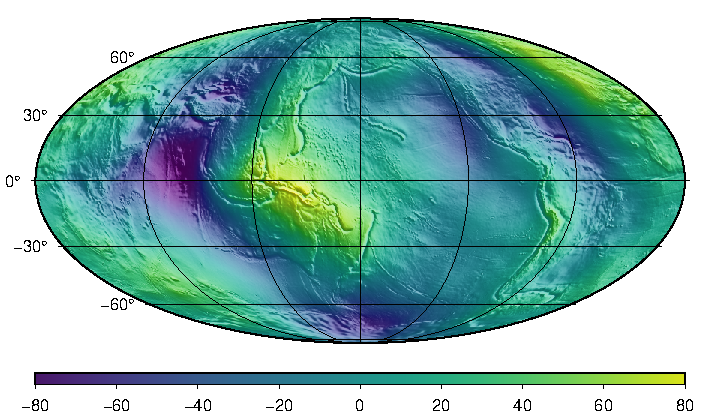
\includegraphics{./fig-geoid-ggm.pdf}
\caption{Výška geoidu na referenčným elipsoidom vypočítaná 
vzťahom~(\ref{eq:geoid_sh}) zo sférického harmonického modelu EIGEN-6C4 do 
stupňa~720 na povrchu elipsoidu~GRS80 (jednotky~m).  Normálne tiažové pole je 
generované ekvipotenciálnym elipsoidom~GRS80.}
\label{fig:geoid_ggm}
\end{figure}

V~praxi sa koeficienty~$\bar{t}_{nk}$ často odhadujú nielen z~anomálií 
tiažového zrýchlenia, ale prakticky zo všetkých dostupných dát, využívajúc 
pritom aj družicové merania.  Výpočet koeficientov~$\bar{t}_{nk}$ z~družicových 
meraní spočíva v~nájdení matematického vzťahu medzi družicovými dátami 
a~niektorou z~veličín gravitačného poľa.  Následne, keďže prakticky každá 
veličina gravitačného poľa môže byť vyjadrená sférickým harmonickým rozvojom, 
je možné získať vzťah medzi meraniami na družici a~neznámymi koeficientmi.  
Uvažujme družicu na nízkej obežnej dráhe Zeme vybavenú GNSS prijímačom, ktorý 
meria polohu družice každú, povedzme, sekundu.  Vieme, že druhou (numerickou) 
deriváciou tejto polohy v~inerciálnom súradnicovom systéme je možné získať 
\emph{výsledne} zrýchlenie pôsobiace na družicu v~danom momente.  
\emph{Parciálne} zrýchlenia, ktoré sú udeľované družici, sú spôsobované 
napríklad tlakom priameho slnečného žiarenia pôsobiaceho na družicu, odporom 
atmosféry či tlakom slnečného žiarenia, ktoré je odrazené od zemského povrchu 
na družicu.  Kľúčovým parciálnym zrýchlením je gravitačné zrýchlenie, ktoré Zem 
udeľuje družici.  Matematickým odstránením všetkých modelovateľných či 
merateľných parciálnych zrýchlení, ktoré nie sú spôsobené gravitačným poľom 
Zeme (medzi takéto zrýchlenia patria aj gravitačné zrýchlenia udelené Mesiacom, 
Slnkom a~planétami Slnečnej sústavy), tak získame dobrú aproximáciu 
gravitačného zrýchlenia, ktoré Zem udeľuje družici.  Spôsobom podobným 
predošlému odseku tak vieme zo sekundového vzorkovania gravitačného zrýchlenia 
vypočítať pomocou rovníc (\ref{eq:vgx_sh}) až~(\ref{eq:vgz_sh}) sférické 
harmonické koeficienty gravitačného poľa Zeme.  V~literatúre sa táto metóda 
nazýva \emph{metóda zrýchlení}.   V~našom regióne sa jej dlhodobo venuje 
skupina pôsobiaca na Astronomickom ústave Akadémie vied Českej republiky 
v~Ond\v{r}ejove.  Táto skupina vyvinula originálny variant metódy zrýchlení 
dosahujúci prvotriednu kvalitu v~celosvetovom meradle 
\parencite{Bezdek2014,encarnacao2020}.  Okrem metódy zrýchlení existuje mnoho 
ďalších prístupov, ktoré využívajú aj ďalšie typy družicových dát 
\parencite[pozri][]{SeeberSatelliteGeodesy}.  Navyše, dokonca aj z~dráhy 
družice je možné odhadnúť koeficienty~$\bar{t}_{nk}$ rozličnými spôsobmi 
\parencite[napríklad][]{Baur2014}.


\subsection{Metódy remove--compute--restore}

Výpočet geoidu vzťahmi~(\ref{eq:stokes_N}) a~(\ref{eq:hotine_N}) je náročný 
nielen z~hľadiska výpočtového času (pozri 
Kapitolu~\ref{sec:stokes_convolution}), ale aj z~pohľadu vstupných dát.  
Všimnime si, že obe rovnice integrujú anomálie, resp. poruchy tiažového 
zrýchlenia na celej sfére~$\sigma$.  Predpokladaná je teda dostupnosť 
gravimetrických meraní na celej Zemi.  Celosvetové gravimetrické databázy síce 
existujú, no v~súčasnosti ich priestorové rozlíšenie dosahuje nanajvýš 
zhruba~$15'$ \parencite{EGM2008,Pail2018}, teda približne~$28$~km na rovníku.  
Táto hustota nepostačuje na dosiahnutie vyžadovanej zhruba centimetrovej 
presnosti geoidu.  Naproti tomu, gravimetrické databázy na úrovni kontinentov 
či štátov sú nezriedka výrazne hustejšie (na Slovensku napríklad~3 až~6 
gravimetrických meraní na~$\textrm{km}^2$, pozri \cite{Kubes2001} 
a~\cite{Zahorec2017}).

Z~podrobných regionálnych anomálií tiažového zrýchlenia sa preto zvykne 
odstrániť (angl.~\emph{remove}) dlhovlnný trend, ktorý je vypočítaný spravidla 
zo sférického harmonického modelu do stupňa~$N$.  Získame tým \emph{reziduálne 
anomálie tiažového zrýchlenia}, ktoré sú následne použité na výpočet 
(angl.~\emph{compute}) \emph{reziduálnej výšky geoidu} nad referenčným 
elipsoidom, napríklad pomocou Stokesovho integrálu.  Na záver je k~získanej 
reziduálnej výške geoidu vrátený (angl.~\emph{restore}) globálny dlhovlnný 
trend geoidu, ktorý je spočítaný opäť zo sférického harmonického modelu.  
Kľúčovou je skutočnosť, že na získanie rozumnej presnosti je postačujúce 
v~prostrednej časti metódy (\emph{compute}) použiť regionálne gravimetrické 
dáta, napríklad do vzdialenosti 100~km od výpočtového bodu.  Integračnou 
oblasťou v~Stokesovom integráli tak už nemusí byť celá sféra~$\sigma$, ale len 
sférický zvrchlík~$\sigma_0$ so stredom vo výpočtovom bode.  Takáto aproximácia 
je možná, pretože vplyv vzdialených \emph{reziduálnych} anomálií tiažového 
zrýchlenia na \emph{reziduálnu} výšku geoidu je s~dostatočnou mierou presnosti 
zanedbateľný, pokiaľ sú stupeň~$N$ a~integračná oblasť~$\sigma_0$ vhodne 
zvolené.

Metóda remove--compute--restore teda umožňuje vhodnú kombináciu vysokej 
lokálnej hustoty regionálnych gravimetrických databáz s~globálnym charakterom 
družicových meraní.  Je potrebné spomenúť, že časť~\emph{compute} môže byť 
realizovaná aj inými metódami výpočtu ako je Stokesov integrál, napríklad 
metódou kolokácie \parencite{MoritzAdvancedGeodesy,MoritzPhysicalGeodesy}.  To 
isté platí v~princípe aj pre časti \emph{remove} a~\emph{restore}, hoci v~tomto 
prípade je použitie sférických harmonických modelov takmer pravidlom.  
Podrobnosti o~metóde remove--compute--restore je možné nájsť napríklad 
v~prácach \textcite{Sjoberg2005} a~\textcite{MoritzPhysicalGeodesy}.

Dodajme aspoň v~stručnosti, že metóda remove--compute--restore sa zvykne 
kombinovať s~metódou reziduálneho terénneho modelu 
\parencite{Forsberg1981,Forsberg1984}.  Táto metóda vychádza zo skutočnosti, že 
tiažové zrýchlenie je veľmi závislé od blízkych hmôt, ktoré sa nachádzajú, 
povedzme, niekoľko desiatok kilometrov od výpočtového bodu (porovnaj 
Obrázky~\ref{fig:gg_grav_sr_2arcsec} a~\ref{fig:h_grav_sr_2arcsec}).  Tvar 
lokálnych hmôt je spravidla dobre popísaný digitálnymi modelmi terénu.  
V~súčasnosti sú bežné modely s~metrovým rozlíšením a~s~vertikálnou presnosťou 
lepšou ako pár desiatok centimetrov.  Podrobnosť týchto modelov je teda výrazne 
vyššia ako podrobnosť terestrických gravimetrických databáz.  Hustota lokálnych 
hmôt sa spravidla považuje za konštantnú (zväčša~$2670\ \mathrm{kg}\, 
\mathrm{m}^{-3}$), no je možné použiť aj presnejšie modely, ak sú dostupné 
\parencite[napríklad][]{Yang2018}.  Metóda reziduálneho terénneho modelu sa 
snaží využiť podrobnosť digitálnych modelov terénu a~výpočtom gravitačného 
účinku takýchto hmôt dopomôcť k~ešte presnejšiemu výpočtu reziduálnych anomálii 
tiažového zrýchlenia.  Tie sa následne využívajú v~metóde 
remove--compute--restore.  Samozrejme, obe metódy môžu byť použité nielen 
s~anomáliami tiažového zrýchlenia, ale aj s~poruchami tiažového zrýchlenia, 
zvislicovými odchýlkami a~ďalšími veličinami fyzikálnej geodézie.




\section{Veningove Meineszove integrály}
\label{sec:vm_integral}

V~Kapitole~\ref{sec:deflections_disturbing_potential} sme ukázali súvislosť 
medzi gravimetrickými zvislicovými odchýlkami a~tiažovým poľom Zeme 
(vzťah~\ref{eq:deflection_grav_s}).  Rovnicu~(\ref{eq:deflection_grav_s}) ale 
spravidla nevieme priamo vypočítať, pretože poruchový potenciál vystupuje vo 
fyzikálnej geodézii väčšinou ako neznáma funkcia 
(Kapitola~\ref{sec:disturbing_potential}).  Jeden zo spôsobov výpočtu 
vzťahu~(\ref{eq:deflection_grav_s}) je pomocou sférického harmonického rozvoja 
poruchového potenciálu (rovnica~\ref{eq:deflection_grav_s_sph}).  V~tejto 
kapitole ukážeme ďalší prístup, ktorý kombinuje geometrickú interpretáciu 
zvislicových odchýlok na geoide (vzťah~\ref{eq:N_deflections}) a~Stokesov 
integrál (vzťah~\ref{eq:stokes_N}).  Kapitola je spracovaná podľa 
\textcite{MoritzPhysicalGeodesy} a~využíva sférickú aproximáciu zvislicových 
odchýlok s~využitím lokálneho kartenziánskeho súradnicového 
systému~$x^\mathrm{s}, y^\mathrm{s}, z^\mathrm{s}$ s~pohyblivým začiatkom 
(pozri Obrázok~\ref{fig:cart_sph}).  Zvislicové odchýlky budeme hľadať na 
geoide, ktorý v~tomto prístupe aproximujeme sférou s~polomerom~$R$ (pozri tiež 
Kapitolu~\ref{sec:stokes_spherical_approximation}).

Vyjadrime z~rovnice~(\ref{eq:N_deflections}) zvislicovú 
odchýlku~$\varepsilon_0$,
%
\begin{equation}
\label{eq:eps0}
\varepsilon_0 = -\frac{\diff N}{\diff s}{.}
\end{equation}
%
Z~Kapitoly~\ref{sec:deflections} vieme, že priemet zvislicovej 
odchýlky~$\varepsilon_0$ môžeme popísať dvoma kolmými zložkami~$\xi_0$ 
a~$\eta_0$, ktoré udávajú vychýlenie zvislice v~smere sever--juh a~v~smere 
východ--západ.  Podobne, $\diff s$~je diferenciál dĺžky v~smere 
priemetu~$\varepsilon_0$.  Potrebujeme preto získať zložky diferenciálu~$\diff 
s$ v~smere meridiánu a~v~smere prvého vertikálu v~lokálnom karteziánskom 
súradnicovom systéme~$x^\mathrm{s}, y^\mathrm{s}, z^\mathrm{s}$ s~pohyblivým 
začiatkom v~tom bode, v~ktorom je určovaná zvislicová odchýlka.  
Z~rovnice~(\ref{eq:diffr2}) 
Prílohy~\ref{app:differential_of_line_element_in_sph_coords} vyplývajú 
nasledovné vzťahy pre zložky diferenciálu~$\diff s$ v~horizontálnej 
rovine~$x^\mathrm{s}, y^\mathrm{s}$,
%
\begin{equation}
\label{eq:ds}
\begin{split}
\diff s_{x^\mathrm{s}} &= R \, \diff \varphi{,}\\
%
\diff s_{y^\mathrm{s}} &= R \, \cos\varphi \, \diff \lambda{.}
\end{split}
\end{equation}
%
Ak je zvislica vychýlená iba v~smere sever--juh, vzťah~(\ref{eq:eps0}) prejde 
do tvaru
%
\begin{equation}
\label{eq:xi0}
\xi_0 = -\frac{\diff N}{\diff s_{x^{\mathrm{s}}}}{.}
\end{equation}
%
Ak je zvislica vychýlená iba v~smere východ--západ, dostaneme vzťah
%
\begin{equation}
\label{eq:lambda0}
\eta_0 = -\frac{\diff N}{\diff s_{y^{\mathrm{s}}}}{.}
\end{equation}
%
Kombináciou rovníc~(\ref{eq:ds}), (\ref{eq:xi0}) a~(\ref{eq:lambda0}) získame 
dve zložky, ktorými je možné popísať zvislicovú odchýlku v~ľubovoľnom smere,
%
\begin{equation}
\begin{split}
\label{eq:xi0_eta0_der}
\xi_0 &= -\frac{1}{R} \, \frac{\partial N}{\partial \varphi}{,}\\
%
\eta_0 &= -\frac{1}{R \, \cos\varphi} \, \frac{\partial N}{\partial \lambda}{.}
\end{split}
\end{equation}
%
Vzťahy~(\ref{eq:xi0_eta0_der}) teda umožňujú vypočítať zvislicové odchýlky na 
geoide zo sklonu geoidu, zatiaľ čo vzťah~(\ref{eq:N_deflections}) umožňuje 
inverzný výpočet sklonu geoidu zo zvislicových odchýlok.

Dosadením Stokesovho integrálu~(\ref{eq:stokes_N}) do 
vzťahov~(\ref{eq:xi0_eta0_der}) získame rovnice
%
\begin{equation}
\label{eq:vm}
\begin{split}
\xi_0 &= -\frac{1}{4\pi\,\gamma_0} \iint\limits_\sigma \frac{\partial 
S(\psi)}{\partial \varphi} \, \Delta g_0 \, \diff\sigma{,}\\
\eta_0 &= -\frac{1}{4\pi \, \gamma_0 \, \cos\varphi} \iint\limits_\sigma 
\frac{\partial S(\psi)}{\partial \lambda} \, \Delta g_0 \, \diff\sigma{.}
\end{split}
\end{equation}
%
Nájdime teraz derivácie~$\partial S(\psi) \slash \partial\varphi$ a~$\partial 
S(\psi) \slash \partial\lambda$.  Z~rovnice~(\ref{eq:stokes_kernel}) vieme, že 
Stokesovo jadro~$S(\psi)$ je funkciou sférickej vzdialenosti~$\psi$.  Tá však 
závisí od sférickej šírky aj od~sférickej dĺžky výpočtového bodu~$(R, \varphi, 
\lambda)$ a~integračného elementu~$(R, \varphi', \lambda')$ 
(vzťah~\ref{eq:cospsi}).  Derivujeme teda zloženú funkciu,
%
\begin{equation}
\label{eq:stokes_kernel_partials}
\begin{split}
\frac{\partial S(\psi)}{\partial \varphi} &= \frac{\diff S(\psi)}{\diff \psi} 
\, \frac{\partial\psi}{\partial\varphi}{,}\\
%
\frac{\partial S(\psi)}{\partial \lambda} &= \frac{\diff S(\psi)}{\diff \psi} 
\, \frac{\partial\psi}{\partial\lambda}{.}\\
\end{split}
\end{equation}
%
Deriváciu~$\diff S(\psi) \slash \diff \psi$ získame derivovaním Stokesovho 
jadra~(\ref{eq:stokes_kernel}) podľa sférickej vzdialenosti~$\psi$.  Na 
získanie parciálnych derivácií~$\partial\psi \slash \partial\varphi$ 
a~$\partial\psi \slash \partial\lambda$ je výhodné diferencovať vzťah pre 
kosínus sférickej šírky (\ref{eq:cospsi}).  Získame tak rovnice
%
\begin{equation}
\label{eq:vm_aux}
\begin{split}
-\sin\psi \, \frac{\partial \psi}{\partial \varphi} &= \cos\varphi \, 
\sin\varphi' - \sin\varphi \, \cos\varphi' \, \cos(\lambda' - \lambda) {,}\\
-\sin\psi \, \frac{\partial \psi}{\partial \lambda} &= \cos\varphi \, 
\cos\varphi' \, \sin(\lambda' - \lambda){.}
\end{split}
\end{equation}
%
Na ďalšiu úpravu rovníc~(\ref{eq:vm_aux}) využime 
vzťahy~(\ref{eq:deflection_aux}), pričom použijeme aktuálnu symboliku, teda 
symboly~$\Theta$, $\phi$, $\Phi$, $\Lambda$ nahradíme symbolmi~$\psi$, 
$\varphi$, $\varphi'$, $\lambda'$ (porovnaj 
Obrázky~\ref{fig:deflections_unit_sphere} a~\ref{fig:surface_integral}),
%
\begin{equation}
\label{eq:vm_aux2}
\begin{split}
\sin\psi \, \cos\alpha &= \cos\varphi \, \sin\varphi' - \sin\varphi \, 
\cos\varphi' \, \cos(\lambda' - \lambda){,}\\
\sin\psi \, \sin\alpha &= \cos\varphi' \, \sin(\lambda' - \lambda){.}
\end{split}
\end{equation}
%
Z~rovníc~(\ref{eq:vm_aux}) a~(\ref{eq:vm_aux2}) vyplývajú vzťahy
%
\begin{equation}
\label{eq:vm_aux3}
\begin{split}
\frac{\partial\psi}{\partial\varphi} &= -\cos\alpha{,}\\
%
\frac{\partial\psi}{\partial\lambda} &= -\cos\varphi \, \sin\alpha{.}
\end{split}
\end{equation}
%
S~využitím~(\ref{eq:stokes_kernel_partials}) a~(\ref{eq:vm_aux3}) dostaneme 
hľadané parciálne derivácie Stokesovho jadra podľa sférickej šírky~$\varphi$ 
a~sférickej dĺžky~$\lambda$,
%
\begin{equation}
\label{eq:stokes_kernel_partials2}
\begin{split}
\frac{S(\psi)}{\partial\varphi} &= -\frac{\diff S(\psi)}{\diff \psi} \, 
\cos\alpha{,}\\
%
\frac{S(\psi)}{\partial\lambda} &= -\frac{\diff S(\psi)}{\diff \psi} \, 
\cos\varphi \, \sin\alpha{.}
\end{split}
\end{equation}
%
Dosadením~(\ref{eq:stokes_kernel_partials2}) do~(\ref{eq:vm}) získame výsledné 
vzťahy
%
\begin{equation}
\label{eq:vm2}
\begin{split}
\xi_0 &= \frac{1}{4\pi\,\gamma_0} \iint\limits_\sigma \frac{\diff 
S(\psi)}{\diff \psi} \, \cos\alpha \, \Delta g_0 \, \diff\sigma{,}\\
\eta_0 &= \frac{1}{4\pi\,\gamma_0} \iint\limits_\sigma \frac{\diff 
S(\psi)}{\diff \psi} \, \sin\alpha \, \Delta g_0 \, \diff\sigma{.}
\end{split}
\end{equation}

Rovnice~(\ref{eq:vm2}) sa nazývajú \emph{Veningove Meineszove integrály}.  
Pomenované sú po holandskom geofyzikovi a~geodetovi F.~A.~Veningovi Meineszovi 
(1887~-- 1966), ktorý ich odvodil v~roku 1928.  Tieto integrály~umožňujú 
výpočet gravimetrických zvislicových odchýlok na geoide z~anomálií tiažového 
zrýchlenia na geoide.  Deriváciu~$\diff S(\psi) \slash \diff\psi$ nebudeme 
podrobne odvádzať a~uvedieme iba jej výsledný tvar
\parencite{MoritzPhysicalGeodesy},
%
\begin{equation}
\frac{\diff S(\psi)}{\diff \psi} = - \frac{\cos\dfrac{\psi}{2}}{2 \, 
\sin^2\dfrac{\psi}{2}} + 8 \, \sin\psi - 6 \, \cos\dfrac{\psi}{2} - 3\, \frac{1 
- \sin\dfrac{\psi}{2}}{\sin\psi} + 3 \, \sin\psi \, \ln \left[ 
\sin\dfrac{\psi}{2} + \sin^2\dfrac{\psi}{2} \right]{.}
\end{equation}

Veningove Meineszove integrály~(\ref{eq:vm2}) patria medzi konvolučné integrály 
(Kapitola~\ref{sec:stokes_convolution}).  Ich integračné jadrá
%
\begin{equation}
\label{eq:vm_kernels}
\frac{\diff S(\psi)}{\diff\psi} \, \cos\alpha{,} \quad \frac{\diff 
S(\psi)}{\diff\psi} \, \sin\alpha
\end{equation}
%
sú singulárne a~homogénne, avšak nie sú izotropné (pozri 
Kapitolu~\ref{sec:stokes_kernel}).  Anizotropnosť je spôsobená závislosťou od 
azimutu~$\alpha$.

Dodajme, že do rovnice~(\ref{eq:xi0_eta0_der}) môže byť dosadený Hotineov 
integrál~(\ref{eq:hotine_N}) namiesto Stokesovho integrálu~(\ref{eq:stokes_N}).  
Získame tým formálne podobné vzťahy, avšak s~integračnými jadrami
%
\begin{equation}
\label{eq:vm_kernels2}
\frac{\diff H(\psi)}{\diff\psi} \, \cos\alpha{,} \quad \frac{\diff 
H(\psi)}{\diff\psi} \, \sin\alpha
\end{equation}
%
a~poruchami tiažového zrýchlenia~$\delta g_0$ namiesto anomálií tiažového 
zrýchlenia~$\Delta g_0$.





% -----------------------------------------------------------------------------

\chapter*{Doslov}

Súčasná geodézia stojí na mnohých pilieroch.  Jedným z~nich je znalosť 
tiažového poľa Zeme.  Vďaka schopnosti merať a~modelovať tiažové pole dokážeme 
určiť mnohé geodetické veličiny presnejšie, než keby sme vplyv tiažového poľa 
neuvažovali.  Príkladom sú korekcie vodorovných uhlov a~dĺžok do~roviny mapy, 
prevýšenia medzi bodmi určené niveláciou či~geocentrické súradnice bodov 
získané GNSS meraniami.  Aby sme lepšie porozumeli geodézii, je výhodné 
pochopiť fyzikálnu podstatu princípov, na ktorých sú geodetické merania 
založené alebo ich implicitne využívajú.  Princípy niektorých geodetických 
metód môžu totiž pôsobiť ako očividné, no až podrobnejším premýšľaním si 
uvedomíme, že táto zrejmosť je len zdanlivá.  Videli sme, že nemalé úsilie si 
vyžaduje opis už i~tak bežných geodetických konceptov, akými sú lokálny 
horizont či smer zavesenej olovnice.  S~pokrokom vedy, výskumu a~technológií sa 
výsledky výskumu tiažového poľa Zeme využívajú čoraz častejšie aj v~bežnej 
geodetickej praxi, hoci to (opäť) nemusí byť na prvý pohlaď zrejmé.  Príkladom 
je určovanie výšky bodu na povrchu Zeme metódami GNSS.  Tie umožňujú vypočítať 
elipsoidickú výšku, teda výšku meranú po normále k~elipsoidu od povrchu 
elipsoidu po daný bod.  Táto výška má geometrický charakter, ktorý nereflektuje 
skutočné tiažové pole Zeme.  Práve z~tohto dôvodu nie je vhodná pre mnohé úlohy 
geodézie, napríklad na vytýčenie \emph{vodorovnej} roviny v~teréne.  Potenciál 
GNSS meraní však v~tejto úlohe predsa len dokážeme využiť, keď si uvedomíme, že 
odčítaním výšky geoidu~$N$ od elipsoidickej výšky~$h$ získame ortometrickú 
výšku~$H^\mathrm{O}$ (Obrázok~\ref{fig:heights}).  Táto výška už má fyzikálny 
charakter, a~tak je rozumnejšie využiť ju na vytýčenie napríklad vodorovnej 
roviny.  V~súčasnosti je takýto prepočet medzi výškami bežnou činnosťou 
geodetov, pričom je uskutočňovaný buď priamo v~GNSS prijímači alebo v~následnom 
spracovaní, niekedy azda i~bez vedomia samotného geodeta.  Porozumieť tiažovému 
poľu Zeme sa teda oplatí.

O~poskytnutie poznatkov, ktoré by napomohli porozumieť základom teórie 
gravitačného a~tiažového poľa, sa snažila aj táto práca.  Niektoré koncepty 
však neboli diskutované vôbec alebo boli spomenuté iba okrajovo.  V~prvom rade, 
práca sa zaoberala určovaním tvaru Zeme v~podobe geoidu.  Molodenského metóda 
určovania fyzického povrchu Zeme (pozri úvodnú kapitolu 
a~Kapitolu~\ref{sec:geoid}) nebola predstavená.  Nie je ale tomu tak preto, že 
táto teória je nedôležitá pre fyzikálnu geodéziu.  Presný opak je pravdou!  
Význam Molodenského teórie v~slovenskom kontexte podčiarkuje aj skutočnosť, že 
práve tento prístup je na Slovensku využívaný na určovanie tvaru Zeme a~jej 
tiažového poľa.  Molodenského koncepcia však presahuje rámec tejto práce a~je 
pokrytá skriptami \textcite{Janak2006}.

Druhou nedotknutou témou je prítomnosť topografických hmôt v~procese určovania 
geoidu.  V~Kapitole~\ref{sec:geoid} sme predpokladali, že vo vonkajšom 
priestore geoidu sa nenachádzajú hmoty.  V~skutočnosti sa vo väčšine 
kontinentálnych častí zemského povrchu nad geoidom nachádzajú topografické 
hmoty, a~to na miestach s~kladnou ortometrickou výškou.  Nad týmito hmotami sa 
ďalej nachádzajú \emph{atmosférické hmoty}.  Aby v~priestore nad geoidom 
platila Laplaceova rovnica, topografické aj atmosférické hmoty je potrebné 
matematicky odstrániť.  Následne je potrebné matematicky zredukovať (pokračovať 
nadol) anomálie tiažového zrýchlenia z~povrchu Zeme (na ktorom boli odmerané) 
na geoid, kde sú potrebné kvôli definovaniu okrajovej podmienky.  Matematické 
odstránenie topografických hmôt a~pokračovanie nadol patria medzi 
najnáročnejšie kroky v~procese určovania geoidu.  Týmto témam sa venuje 
napríklad práca \textcite{Janak2006}.

Pre názornosť sme v~Kapitole~\ref{sec:spherical_harmonic_expansion} často 
prirovnávali vlastnosti sférických harmonických funkcií k~vlastnostiam 
jednotkových vektorov.  Hlbšie porozumieť sférickým harmonickým funkciám a~ich 
vlastnostiam je možné napríklad pomocou \emph{funkcionálnej analýzy}.  
Funkcionálna analýza je pomerne abstraktná časť matematiky, ktorá ale 
v~súčasnosti nie je zaradená do obsahu študijného programu Geodézia 
a~kartografia na Stavebnej fakulte Slovenskej technickej univerzity 
v~Bratislave.  Využívali sme preto prirovnania k~jednotkovým vektorom, ktoré 
majú v~širšom zmysle mnoho podobných vlastností ako sférické harmonické funkcie 
a~navyše sú jednoducho predstaviteľné.  Základy funkcionálnej analýzy je možné 
nájsť napríklad v~práci~\textcite{Janak2006}.  Podrobnejšie informácie je možné 
nájsť napríklad v~knihe~\textcite{Rektorys}, ktorá je napísaná v~češtine 
a~svojou formou je prístupná aj~inžinierom a~fyzikom.  Odporúčať tiež môžeme 
geodetickú literatúru v~anglickom jazyku, napríklad 
\textcite{MoritzAdvancedGeodesy}, \textcite{SansoGeoidDetermination}, 
\textcite{Borre2006} či \textcite{Freeden2009}.

Zrejme nebudeme ďaleko od pravdy, keď budeme tvrdiť, že vedecká a~akademická 
literatúra, nevynímajúc tieto strany, sa v~istom zmysle rodí veľmi ťažko.  
Objavovať poznatky je totiž zložité, rovnako ako je náročné sa ich snažiť 
sprostredkovať čitateľovi, ktorý nevybočuje z~tohto začarovaného kruhu a~pre 
porozumenie textu musí neraz vynaložiť podobné alebo aj väčšie úsilie ako 
samotný autor.  Mohli by sme teda povedať, že ide tak trochu o~vzájomnú hru, 
ktorá, pokiaľ sa hrá s~otvorenou mysľou, spravidla stojí za to.





% -----------------------------------------------------------------------------

\appendix
\chapter{Numerická aplikácia operátora gradient}
\label{app:numerical_application_of_gradient}

Uvažujme dvojrozmerný karteziánsky súradnicový systém so súradnicovými osami 
$x, y$.  Nech $f(x, y)$ je skalárna funkcia dvoch premenných daná vzťahom
%
\begin{equation}
\label{eq:f}
f(x, y) = \sin(2x) + \cos(2y){.}
\end{equation}
%
Aplikáciou operátora gradient na skalárnu funkciu $f(x, y)$ získame v~zmysle
rovnice~(\ref{eq:gradient}) vektorovú funkciu
%
\begin{equation}
\label{eq:gradf}
\nabla f(x, y) =
\begin{bmatrix}
\dfrac{\partial f(x, y)}{\partial x} \\[2ex]
\dfrac{\partial f(x, y)}{\partial y}
\end{bmatrix}
=
\begin{bmatrix}
2 \cos(2x) \\[2ex]
-2 \sin(2y)
\end{bmatrix}
{.}
\end{equation}

Ukážka numerického výpočtu funkcie~(\ref{eq:f}) a~jej 
gradientu~(\ref{eq:gradf}) na~intervale $x, y \in [-1, 1]$ je uvedená 
v~Zdrojovom~kóde~\ref{src:f_gradf}.  Grafické znázornenie je uvedené na 
Obrázku~\ref{fig:f_gradf}.  Všímajme si smer šípky a~jej veľkosť v~závislosti 
od polohy a~pokúsme sa danú situáciu interpretovať.

\vspace{2ex}

\lstinputlisting[caption=Výpočet a~zobrazenie funkcie dvoch premenných a~jej
gradientu v~programovacom jazyku Python, language=mypython, label=src:f_gradf,
captionpos=t]{../python/gradient.py}

\begin{figure}[bt]
\centering
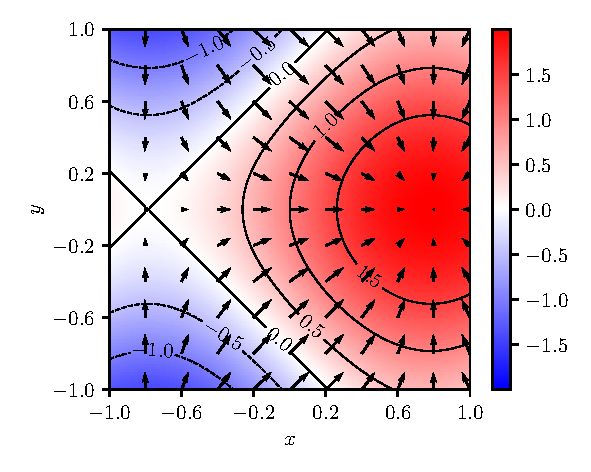
\includegraphics{./fig-gradient.pdf}
\caption{Skalárna funkcia $f(x, y) = \sin(2x) + \cos(2y)$ a~jej gradient 
$\nabla f(x, y)$ na~intervale $x, y \in [-1, 1]$.  Skalárna funkcia je 
znázornená hypsometricky a~izočiarami.  Gradient je zobrazený orientovanými 
šípkami, pričom šípka udáva smer a~veľkosť najväčšieho nárastu funkcie $f(x, 
y)$ v~danom bode.}
\label{fig:f_gradf}
\end{figure}






\chapter{Operátor gradient v~ortogonálnych súradnicových systémoch}
\label{app:gradient_in_orthogonal_systems}

V~tejto kapitole je vyjadrený operátor gradient v~ortogonálnych súradnicových 
systémoch.  \emph{Ortogonálny súradnicový systém} je taký súradnicový systém, 
ktorého súradnicové plochy sa pretínajú pod pravým uhlom.  Príkladom sú 
karteziánske súradnicové systémy~$x, y, z$ a~$x^\mathrm{s}, y^\mathrm{s}, 
z^\mathrm{s}$ či~krivočiary systém súradníc~$r, \varphi, \lambda$ (pozri 
Obrázok~\ref{fig:cart_sph}).

V~Kapitole~\ref{app:gradient_in_spherical_coordinates} je odvodený operátor 
gradient~(\ref{eq:gradient_sph}) v~ortogonálnom krivočiarom sférickom 
súradnicovom systéme~$(r, \varphi, \lambda)$.  
V~Kapitole~\ref{app:gradient_in_orthogonal_coordinates} je uvedené všeobecné 
riešenie pre ľubovoľný ortogonálny súradnicový systém.



\section{Operátor gradient vo sférickom súradnicovom systéme}
\label{app:gradient_in_spherical_coordinates}

Nech~$f$ je skalárna diferencovateľná funkcia.  V~lokálnom karteziánskom 
súradnicovom systéme $x^{\mathrm{s}}, y^{\mathrm{s}}, z^{\mathrm{s}}$ 
s~jednotkovými vektormi $\vec e^\mathrm{s}_1, \vec e^\mathrm{s}_2, \vec 
e^\mathrm{s}_3$ (Obrázok~\ref{fig:cart_sph}) je gradient funkcie~$f$ daný 
vzťahom~(\ref{eq:gradient}),
%
\begin{equation}
\nabla f = \vec e^\mathrm{s}_1 \, \frac{\partial f}{\partial x^{\mathrm{s}}} 
+ \vec e^\mathrm{s}_2 \, \frac{\partial f}{\partial y^{\mathrm{s}}} + \vec 
e^\mathrm{s}_3 \, \frac{\partial f}{\partial z^{\mathrm{s}}}{.}
\end{equation}
%
Cieľom tejto kapitoly je vyjadriť parciálne derivácie $\partial f \slash 
\partial x^{\mathrm{s}}, \partial f \slash \partial y^{\mathrm{s}}, \partial 
f \slash \partial z^{\mathrm{s}}$ pomocou ortogonálnych \emph{krivočiarych} 
súradníc $\varphi, \lambda, r$.

Je zrejmé, že potrebujeme nájsť parciálne derivácie $\partial f \slash \partial 
\varphi, \partial f \slash \partial \lambda, \partial f \slash \partial r$.  
Túto úlohu komplikuje závislosť karteziánskych súradníc $x, y, z$ od sférických 
súradníc $\varphi, \lambda, r$ (pozri rovnice~\ref{eq:sph2cart}).  Derivujeme 
preto zloženú funkciu troch premenných,
%
\begin{equation}
\label{eq:f_partials_rlatlon}
\begin{split}
\frac{\partial f}{\partial \varphi} &= \frac{\partial f}{\partial x} \, 
\frac{\partial x}{\partial \varphi} + \frac{\partial f}{\partial y} \, 
\frac{\partial y}{\partial \varphi} + \frac{\partial f}{\partial z} \, 
\frac{\partial z}{\partial \varphi}{,}\\
%
\frac{\partial f}{\partial \lambda} &= \frac{\partial f}{\partial x} \, 
\frac{\partial x}{\partial \lambda} + \frac{\partial f}{\partial y} \, 
\frac{\partial y}{\partial \lambda} + \frac{\partial f}{\partial z} \, 
\frac{\partial z}{\partial \lambda}{,}\\
%
\frac{\partial f}{\partial r} &= \frac{\partial f}{\partial x} \, 
\frac{\partial x}{\partial r} + \frac{\partial f}{\partial y} \, \frac{\partial 
y}{\partial r} + \frac{\partial f}{\partial z} \, \frac{\partial z}{\partial 
r}{.}
\end{split}
\end{equation}
%
Rovnicu~(\ref{eq:f_partials_rlatlon}) môžeme zapísať v~maticovom tvare
%
\begin{equation}
\label{eq:f_partials_rlatlon_2}
\begin{bmatrix}
\dfrac{\partial f}{\partial \varphi}\\[2ex]
\dfrac{\partial f}{\partial \lambda}\\[2ex]
\dfrac{\partial f}{\partial r}
\end{bmatrix}
%
=
%
\begin{bmatrix}
\dfrac{\partial x}{\partial \varphi} & \dfrac{\partial y}{\partial \varphi} 
& \dfrac{\partial z}{\partial \varphi}\\[2ex]
\dfrac{\partial x}{\partial \lambda} & \dfrac{\partial y}{\partial \lambda
} & \dfrac{\partial z}{\partial \lambda}\\[2ex]
\dfrac{\partial x}{\partial r} & \dfrac{\partial y}{\partial r} 
& \dfrac{\partial z}{\partial r}
\end{bmatrix}
%
\,
%
\begin{bmatrix}
\dfrac{\partial f}{\partial x}\\[2ex]
\dfrac{\partial f}{\partial y}\\[2ex]
\dfrac{\partial f}{\partial z}
\end{bmatrix}
%
{.}
\end{equation}

Zaveďme vektorovú funkciu~$\vec r$, ktorá bude popisovať začiatok lokálneho 
súradnicového systému $x^\mathrm{s}, y^\mathrm{s}, z^\mathrm{s}$ v~globálnom 
súradnicovom systéme $x, y, z$ (rovnice~\ref{eq:sph2cart}),
%
\begin{equation}
\label{eq:vector_r}
\vec r =
%
\begin{bmatrix}
x(\varphi, \lambda, r)\\
y(\varphi, \lambda, r)\\
z(\varphi, r)
\end{bmatrix}
%
=
%
\begin{bmatrix}
r \, \cos\varphi \, \cos\lambda\\
r \, \cos\varphi \, \sin\lambda\\
r \, \sin\varphi
\end{bmatrix}
%
{.}
\end{equation}
%
Vzťah~(\ref{eq:f_partials_rlatlon_2}) potom môžeme prepísať do tvaru
%
\begin{equation}
\label{eq:grad_cart2sph}
\begin{bmatrix}
\dfrac{\partial f}{\partial \varphi}\\[2ex]
\dfrac{\partial f}{\partial \lambda}\\[2ex]
\dfrac{\partial f}{\partial r}
\end{bmatrix}
%
=
%
\begin{bmatrix}
\left( \hat{\vec e}_1^\mathrm{s} \right)^\top\\
\left( \hat{\vec e}_2^\mathrm{s} \right)^\top\\
\left( \hat{\vec e}_3^\mathrm{s} \right)^\top
\end{bmatrix}
%
\,
%
\begin{bmatrix}
\dfrac{\partial f}{\partial x}\\[2ex]
\dfrac{\partial f}{\partial y}\\[2ex]
\dfrac{\partial f}{\partial z}
\end{bmatrix}
%
{,}
\end{equation}
%
kde symboly
%
\begin{equation}
\label{eq:er_elat_elon}
\hat{\vec e}_1^\mathrm{s} = \frac{\partial \vec r}{\partial \varphi} = 
%
\begin{bmatrix}
-r \, \sin\varphi \, \cos\lambda\\
-r \, \sin\varphi \, \sin\lambda\\
r \, \cos\varphi
\end{bmatrix}
%
{,}\quad
%
\hat{\vec e}_2^\mathrm{s} = \frac{\partial \vec r}{\partial \lambda} = 
%
\begin{bmatrix}
-r \, \cos\varphi \, \sin\lambda\\
r \, \cos\varphi \, \cos\lambda\\
0
\end{bmatrix}
%
{,}\quad
%
\hat{\vec e}_3^\mathrm{s} = \frac{\partial \vec r}{\partial r} = 
%
\begin{bmatrix}
\cos\varphi \, \cos\lambda\\
\cos\varphi \, \sin\lambda\\
\sin\varphi
\end{bmatrix}
%
\end{equation}
%
predstavujú vektory v~smere osí $x^{\mathrm{s}}, y^{\mathrm{s}}, 
z^{\mathrm{s}}$ lokálneho karteziánskeho súradnicového systému.  
Derivácie~$\partial f \slash \partial x, \partial f \slash \partial y, \partial 
f \slash \partial z$ vyjadríme pomocou parciálnych derivácií $\partial f \slash 
\partial \varphi, \partial f \slash \partial \lambda, \partial f \slash 
\partial r$ vyriešením systému lineárnych rovníc~(\ref{eq:grad_cart2sph}) 
použitím niektorej z~metód lineárnej algebry.

Obzvlášť jednoduchá metóda riešenia systému rovníc~(\ref{eq:grad_cart2sph}) je 
nasledovná.  Normovaním vektorov~(\ref{eq:er_elat_elon}) ich veľkosťami
%
\begin{equation}
\begin{aligned}
\| \hat{\vec e}_1^\mathrm{s} \| &= \sqrt{(-r \, \sin\varphi \, \cos\lambda)^2 
+ (-r \, \sin\varphi \, \sin\lambda)^2 + (r \, \cos\varphi)^2} = r{,}\\
%
\| \hat{\vec e}_2^\mathrm{s} \| &= \sqrt{(-r \, \cos\varphi \, \sin\lambda)^2 
+ (r \, \cos\varphi \, \cos\lambda)^2} = r \, \cos\varphi{,}\\
%
\| \hat{\vec e}_3^\mathrm{s} \| &= \sqrt{(\cos\varphi \, \cos\lambda)^2 
+ (\cos\varphi \, \sin\lambda)^2 + \sin^2\varphi} = 1
%
\end{aligned}
\end{equation}
%
získame jednotkové vektory v~smere súradnicových osí~$x^\mathrm{s}, 
y^\mathrm{s}, z^\mathrm{s}$,
%
\begin{equation}
\label{eq:er_elat_elon_unit}
%
\vec e^\mathrm{s}_1 = \frac{\hat{\vec e}_1^\mathrm{s}}{\| \hat{\vec 
e}_1^\mathrm{s} \|} = 
%
\begin{bmatrix}
-\sin\varphi \, \cos\lambda\\
-\sin\varphi \, \sin\lambda\\
\cos\varphi
\end{bmatrix}
%
{,}\quad
%
\vec e^\mathrm{s}_2 = \frac{\hat{\vec e}_2^\mathrm{s}}{\| \hat{\vec 
e}_2^\mathrm{s} \|} = 
%
\begin{bmatrix}
-\sin\lambda\\
\cos\lambda\\
0
\end{bmatrix}
%
{,}\quad
%
\vec e^\mathrm{s}_3 = \frac{\hat{\vec e}_3^\mathrm{s}}{\| \hat{\vec 
e}_3^\mathrm{s} \|} = 
%
\begin{bmatrix}
\cos\varphi \, \cos\lambda\\
\cos\varphi \, \sin\lambda\\
\sin\varphi
\end{bmatrix}
%
{.}
%
\end{equation}
%
Systém lineárnych rovníc~(\ref{eq:grad_cart2sph}) potom môžeme prepísať do 
tvaru
%
\begin{equation}
\label{eq:grad_cart2sph_2}
\begin{bmatrix}
\dfrac{\partial f}{\partial \varphi}\\[2ex]
\dfrac{\partial f}{\partial \lambda}\\[2ex]
\dfrac{\partial f}{\partial r}
\end{bmatrix}
%
=
%
\begin{bmatrix}
r \, \left( \vec e^\mathrm{s}_1\right)^\top\\
r \, \cos\varphi \, \left(\vec e^\mathrm{s}_2\right)^\top\\
\left(\vec e^\mathrm{s}_3\right)^\top
\end{bmatrix}
%
\,
%
\begin{bmatrix}
\dfrac{\partial f}{\partial x}\\[2ex]
\dfrac{\partial f}{\partial y}\\[2ex]
\dfrac{\partial f}{\partial z}
\end{bmatrix}
%
{.}
\end{equation}
%
O~vektoroch $\vec e^\mathrm{s}_1, \vec e^\mathrm{s}_2, \vec e^\mathrm{s}_3$ 
vieme, že sú ortogonálne (pozri rovnicu~\ref{eq:ei_orthogonality}) a~ich 
veľkosť je rovná~$1$, čo možno overiť vzťahmi~(\ref{eq:er_elat_elon_unit}).  
Inverzia matice systému lineárnych rovníc~(\ref{eq:grad_cart2sph_2}) je potom 
daná vzťahom \parencite{MichelLectures}
%
\begin{equation}
\begin{bmatrix}
r \, \left( \vec e^\mathrm{s}_1 \right)^\top\\[2ex]
r \, \cos\varphi \, \left( \vec e^\mathrm{s}_2 \right)^\top\\[2ex]
\left( \vec e^\mathrm{s}_3 \right)^\top
\end{bmatrix}^{-1}
%
=
%
\begin{bmatrix}
\dfrac{1}{r} \, \vec e^\mathrm{s}_1 \quad \dfrac{1}{r \, \cos\varphi} \, \vec 
e^\mathrm{s}_2 \quad \vec e^\mathrm{s}_3
\end{bmatrix}
{.}
\end{equation}
%
Riešenie rovnice~(\ref{eq:grad_cart2sph_2}) má teda tvar
%
\begin{equation}
\label{eq:grad_cart2sph_3}
\begin{bmatrix}
\dfrac{\partial f}{\partial x}\\[2ex]
\dfrac{\partial f}{\partial y}\\[2ex]
\dfrac{\partial f}{\partial z}
\end{bmatrix}
%
=
%
\begin{bmatrix}
\dfrac{1}{r} \, \vec e^\mathrm{s}_1 \quad \dfrac{1}{r \, \cos\varphi} \, \vec 
e^\mathrm{s}_2 \quad \vec e^\mathrm{s}_3
\end{bmatrix}
%
\,
%
\begin{bmatrix}
\dfrac{\partial f}{\partial \varphi}\\[2ex]
\dfrac{\partial f}{\partial \lambda}\\[2ex]
\dfrac{\partial f}{\partial r}
\end{bmatrix}
%
{.}
\end{equation}
%
Hľadané parciálne derivácie v~súradnicovom systéme~$x^\mathrm{s}, y^\mathrm{s}, 
z^\mathrm{s}$ sú tak dané vzťahmi
%
\begin{equation}
\label{eq:lnof_diff_oeprators}
\begin{split}
\frac{\partial f}{\partial x^\mathrm{s}} &= \frac{1}{r} \, \frac{\partial 
f}{\partial \varphi}{,}\\
%
\frac{\partial f}{\partial y^\mathrm{s}} &= \frac{1}{r \, \cos\varphi} \, 
\frac{\partial f}{\partial \lambda}{,}\\
%
\frac{\partial f}{\partial z^\mathrm{s}} &= \frac{\partial f}{\partial r}{.}
\end{split}
\end{equation}
%
Keďže funkcia~$f$ je podľa predpokladu ľubovoľná skalárna diferencovateľná 
funkcia, vzťah~(\ref{eq:grad_cart2sph_3}) dokazuje 
rovnicu~(\ref{eq:gradient_sph}).




\section{Operátor gradient v~ortogonálnom súradnicovom systéme}
\label{app:gradient_in_orthogonal_coordinates}

Odvodenie z~predošlej kapitoly možno zovšeobecniť na ľubovoľný ortogonálny 
súradnicový systém.  Nech~$\xi_1, \xi_2, \xi_3$ je ortogonálny súradnicový 
systém a~nech~$f$ je diferencovateľná funkcia.  Gradient funkcie~$f$ je v~tomto 
súradnicovom systéme daný vzťahom 
\parencite{Arfken2005,SansoGeoidDetermination}
%
\begin{equation}
\label{eq:grad_orthogonal_system}
\nabla f = \sum_{i = 1}^3 \frac{\hat{\vec e}_i}{\| \hat{\vec e}_i \|^2} \, 
\frac{\partial f}{\partial \xi_i} = \sum_{i = 1}^3 \frac{1}{\| \hat{\vec e}_i 
\|} \, \vec e_i \, \frac{\partial f}{\partial \xi_i}{,}
\end{equation}
%
kde
%
\begin{equation}
\label{eq:xi1xi2xi3_vectors}
\hat{\vec e}_i = \frac{\partial \vec r(\boldsymbol \xi)}{\partial \xi_i}
\end{equation}
%
je vektor v~smere súradnicovej osi~$\xi_i$,
%
\begin{equation}
\label{eq:xi1xi2xi3_unit_vectors}
\vec e_i = \frac{\hat{\vec e}_i}{\| \hat{\vec e}_i \|}
\end{equation}
%
je jednotkový vektor v~smere súradnicovej osi~$\xi_i$~a
%
\begin{equation}
\boldsymbol \xi =
%
\begin{bmatrix}
\xi_1\\
\xi_2\\
\xi_3
\end{bmatrix}
%
{.}
%
\end{equation}






\chapter{Laplaceov operátor v~ortogonálnych súradnicových systémoch}
\label{app:laplace_in_spherical_coordinates}

V~Kapitole~\ref{app:laplace_in_spherical_system} je odvodený tvar Laplaceovho 
operátora vo sférickom súradnicovom systéme (rovnica~\ref{eq:vg_laplace_sph}).  
V~Kapitole~\ref{app:laplace_in_orthogonal_coordinates} je odvodený všeobecný 
tvar Laplaceovho operátora v~ľubovoľnom ortogonálnom súradnicovom systéme.  
Kapitola~\ref{app:laplace_in_spherical_system} je spracovaná 
podľa~\textcite{MichelLectures} 
a~Kapitola~\ref{app:laplace_in_orthogonal_coordinates} 
podľa~\textcite{SansoGeoidDetermination}.


\section{Laplaceov operátor vo sférickom súradnicovom systéme}
\label{app:laplace_in_spherical_system}

Aplikujme operátor gradient vo sférických súradniciach~(\ref{eq:gradient_sph}) 
na dvakrát diferencovateľnú funkciu~$f$ v~zmysle 
rovnice~(\ref{eq:laplace_cart_grad_grad_notation}),
%
\begin{align}
\label{eq:grad_grad_sph}
\nabla^2 f &= \nabla \cdot \left( \nabla f \right)\nonumber\\
%
&= \left( \vec e_1^\mathrm{s} \, \frac{1}{r} \, \frac{\partial}{\partial 
\varphi} + \vec e_2^\mathrm{s} \, \frac{1}{r \, \cos\varphi} \, 
\frac{\partial}{\partial \lambda} + \vec e_3^\mathrm{s} 
\frac{\partial}{\partial r} \right) \cdot \left( \vec e_1^\mathrm{s} \, 
\frac{1}{r} \, \frac{\partial f}{\partial \varphi} + \vec e_2^\mathrm{s} \, 
\frac{1}{r \, \cos\varphi} \, \frac{\partial f}{\partial \lambda} + \vec 
e_3^\mathrm{s} \frac{\partial f}{\partial r} \right)\nonumber\displaybreak[2]\\
%
&= \frac{1}{r^2} \, \underbrace{\vec e^\mathrm{s}_1 \cdot \frac{\partial \vec 
e^\mathrm{s}_1}{\partial \varphi}}_{\vec e_1^\mathrm{s} \cdot (- \vec 
e_3^\mathrm{s}) = 0} \, \frac{\partial f}{\partial \varphi} + \frac{1}{r^2} \, 
\underbrace{\vec e^\mathrm{s}_1 \cdot \vec e^\mathrm{s}_1}_{1} \, 
\frac{\partial^2 f}{\partial \varphi^2} + \frac{1}{r^2 \, \cos\varphi} \, 
\underbrace{\vec e_1^\mathrm{s} \cdot \frac{\partial \vec 
e_2^\mathrm{s}}{\partial \varphi}}_{\vec e_1^\mathrm{s} \cdot \vec 0 = 0} \, 
\frac{\partial f}{\partial \lambda}\nonumber\displaybreak[2]\\
%
&\phantom{={}}+ \frac{1}{r^2} \, \underbrace{\vec e_1^\mathrm{s} \cdot \vec 
e_2^\mathrm{s}}_{0} \, \frac{\partial}{\partial \varphi} \left( 
\frac{1}{\cos\varphi} \right) \, \frac{\partial f}{\partial \lambda} 
+ \frac{1}{r^2 \, \cos\varphi} \, \underbrace{\vec e_1^\mathrm{s} \cdot \vec 
e_2^\mathrm{s}}_{0} \, \frac{\partial^2 f}{\partial \varphi \, \partial 
\lambda} + \frac{1}{r} \, \underbrace{\vec e_1^\mathrm{s} \cdot \frac{\partial 
\vec e_3^\mathrm{s}}{\partial \varphi}}_{\vec e_1^\mathrm{s} \cdot \vec 
e_1^\mathrm{s} = 1} \, \frac{\partial f}{\partial r}\nonumber\displaybreak[2]\\
%
&\phantom{={}}+ \frac{1}{r} \, \underbrace{\vec e_1^\mathrm{s} \cdot \vec 
e_3^\mathrm{s}}_{0} \, \frac{\partial^2 f}{\partial \varphi \, \partial r} 
+ \frac{1}{r^2 \, \cos\varphi} \, \underbrace{\vec e_2^\mathrm{s} \cdot 
\frac{\partial \vec e_1^\mathrm{s}}{\partial \lambda}}_{\vec e_2^\mathrm{s} 
\cdot (-\sin\varphi \, \vec e_2^\mathrm{s}) = -\sin\varphi} \, \frac{\partial 
f}{\partial \varphi} + \frac{1}{r^2 \, \cos\varphi} \, \underbrace{\vec 
e_2^\mathrm{s} \cdot \vec e_1^\mathrm{s}}_{0} \, \frac{\partial^2 f}{\partial 
\lambda \, \partial \varphi}\displaybreak[2]\\
%
&\phantom{={}}+ \frac{1}{r^2 \, \cos^2\varphi} \, \underbrace{\vec 
e_2^\mathrm{s} \cdot \frac{\partial \vec e_2^\mathrm{s}}{\partial \lambda}}_{0} 
\, \frac{\partial f}{\partial\lambda} + \frac{1}{r^2 \, \cos^2\varphi} \, 
\underbrace{\vec e_2^\mathrm{s} \cdot \vec e_2^\mathrm{s}}_{1} \, 
\frac{\partial^2 f}{\partial\lambda^2} + \frac{1}{r \, \cos\varphi} \, 
\underbrace{\vec e_2^\mathrm{s} \cdot \frac{\partial \vec 
e_3^\mathrm{s}}{\partial \lambda}}_{\vec e_2^\mathrm{s} \cdot (\cos\varphi \, 
\vec e_2^\mathrm{s}) = \cos\varphi} \, \frac{\partial f}{\partial 
r}\nonumber\displaybreak[2]\\
%
&\phantom{={}}+ \frac{1}{r \, \cos\varphi} \, \underbrace{\vec e_2^\mathrm{s} 
\cdot \vec e_3^\mathrm{s}}_{0} \, \frac{\partial^2 f}{\partial \lambda \, 
\partial r} + \frac{1}{r} \, \underbrace{\vec e_3^\mathrm{s} \cdot 
\frac{\partial \vec e_1^\mathrm{s}}{\partial r}}_{\vec e_3^\mathrm{s} \cdot 
\vec 0 = 0} \, \frac{\partial f}{\partial \varphi} + \underbrace{\vec 
e_3^\mathrm{s} \cdot \vec e_1^\mathrm{s}}_{0} \, \frac{\partial}{\partial r} 
\left( \frac{1}{r} \right) \, \frac{\partial f}{\partial \varphi} 
+ \underbrace{\vec e_3^\mathrm{s} \cdot \vec e_1^\mathrm{s}}_{0} \, \frac{1}{r} 
\, \frac{\partial^2 f}{\partial r \, \partial 
\varphi}\nonumber\displaybreak[2]\\
%
&\phantom{={}}+\frac{1}{r \, \cos\varphi} \, \underbrace{\vec e_3^\mathrm{s} 
\cdot \frac{\partial \vec e_2^\mathrm{s}}{\partial r}}_{\vec e_3^\mathrm{s} 
\cdot \vec 0 = 0} \, \frac{\partial f}{\partial \lambda} + \underbrace{\vec 
e_3^\mathrm{s} \cdot \vec e_2^\mathrm{s}}_{0} \, \frac{\partial}{\partial r} 
\left( \frac{1}{r \, \cos\varphi} \right) \, \frac{\partial f}{\partial 
\lambda} + \underbrace{\vec e_3^\mathrm{s} \cdot \vec e_2^\mathrm{s}}_{0} \, 
\frac{1}{r \, \cos\varphi} \, \frac{\partial^2 f}{\partial r \, \partial 
\lambda}\nonumber\displaybreak[2]\\
%
&\phantom{={}}+ \underbrace{\vec e_3^\mathrm{s} \cdot \frac{\partial \vec 
e_3^\mathrm{s}}{\partial r}}_{\vec e_3^\mathrm{s} \cdot \vec 0 = 0} \, 
\frac{\partial f}{\partial r} + \underbrace{\vec e_3^\mathrm{s} \cdot \vec 
e_3^\mathrm{s}}_{1} \, \frac{\partial^2 f}{\partial r^2}{.}\nonumber
\end{align}
%
Jednotkové vektory $\vec e_1^\mathrm{s}, \vec e_2^\mathrm{s}, \vec 
e_3^\mathrm{s}$ z~predošlej rovnice sú dané 
vzťahmi~(\ref{eq:er_elat_elon_unit}).  Ich derivácie podľa sférických súradníc 
majú nasledovný tvar,
%
\begin{alignat}{3}
&\frac{\partial \vec e_1^\mathrm{s}}{\partial \varphi} =
%
\begin{bmatrix}
-\cos\varphi \, \cos\lambda\\
-\cos\varphi \, \sin\lambda\\
-\sin\varphi\\
\end{bmatrix}
%
= -\vec e_3^\mathrm{s}
%
{,}\quad
%
&&\frac{\partial \vec e_1^\mathrm{s}}{\partial \lambda} =
%
\begin{bmatrix}
 \sin\varphi \, \sin\lambda\\
-\sin\varphi \, \cos\lambda\\
0\\
\end{bmatrix}
%
= -\sin\varphi \, \vec e_2^\mathrm{s}
%
{,}\quad
%
&&\frac{\partial \vec e_1^\mathrm{s}}{\partial r} = \vec 0{,}\nonumber\\
%
\label{eq:er_elat_elon_unit_derivatives}
&\frac{\partial \vec e_2^\mathrm{s}}{\partial \varphi} = \vec 0{,}
%
&&\frac{\partial \vec e_2^\mathrm{s}}{\partial \lambda} =
%
\begin{bmatrix}
-\cos\lambda\\
-\sin\lambda\\
0\\
\end{bmatrix}
%
{,}
%
&&\frac{\partial \vec e_2^\mathrm{s}}{\partial r} = \vec 0{,}\\
%
&\frac{\partial \vec e_3^\mathrm{s}}{\partial \varphi} =
%
\begin{bmatrix}
-\sin\varphi \, \cos\lambda\\
-\sin\varphi \, \sin\lambda\\
\cos\varphi\\
\end{bmatrix}
%
= \vec e_1^\mathrm{s}
%
{,}
%
&&\frac{\partial \vec e_3^\mathrm{s}}{\partial \lambda} =
%
\begin{bmatrix}
-\cos\varphi \, \sin\lambda\\
 \cos\varphi \, \cos\lambda\\
0\\
\end{bmatrix}
%
= \cos\varphi \, \vec e_2^\mathrm{s}
%
{,}
%
&&\frac{\partial \vec e_3^\mathrm{s}}{\partial r} = \vec 0{.}
\nonumber
\end{alignat}
%
Kombináciou rovníc~(\ref{eq:grad_grad_sph}) 
a~(\ref{eq:er_elat_elon_unit_derivatives}) získame Laplaceov operátor vo 
sférických súradniciach,
%
\begin{equation}
\label{eq:laplace_sph}
\nabla^2 f = \frac{1}{r^2} \frac{\partial}{\partial r} \left( r^2
\frac{\partial f}{\partial r} \right) + \frac{1}{r^2 \, \cos\varphi}
\frac{\partial}{\partial \varphi} \left( \cos\varphi \frac{\partial f}{\partial 
\varphi} \right) + \frac{1}{r^2 \,
\cos^2\varphi}\frac{\partial^2 f}{\partial \lambda^2}{.}
\end{equation}




\section{Laplaceov operátor v~ortogonálnom súradnicovom systéme}
\label{app:laplace_in_orthogonal_coordinates}

Odvodenie z~Kapitoly~\ref{app:laplace_in_spherical_system} možno zovšeobecniť 
na ľubovoľný ortogonálny súradnicový systém~$\xi_1, \xi_2, \xi_3$.

Nech~$f$ je dvakrát diferencovateľná funkcia.  Všeobecný tvar Laplaceovho 
operátora získame pomocou rovníc~(\ref{eq:laplace_cart_grad_grad_notation}) 
a~(\ref{eq:grad_orthogonal_system}),
%
\begin{equation}
\label{eq:laplace_orthogonal_system_1}
\begin{split}
\nabla^2 f &= \nabla \cdot \left( \nabla f \right) = \left( \sum_{i = 1}^3 
\frac{\hat{\vec e}_i}{\| \hat{\vec e}_i \|^2} \, \frac{\partial}{\partial 
\xi_i}\right) \cdot \left( \sum_{j = 1}^3 \frac{\hat{\vec e}_j}{\| \hat{\vec 
e}_j \|^2} \, \frac{\partial f}{\partial \xi_j}
\right)\\
%
&= \sum_{i = 1}^{3} \sum_{j = 1}^3 \frac{1}{\| \hat{\vec e}_i \|^2 \, \| 
\hat{\vec e}_j \|^2} \, \hat{\vec e}_i \cdot \frac{\partial \hat{\vec 
e}_j}{\partial \xi_i} \, \frac{\partial f}{\partial \xi_j}
- 2\, \sum_{i = 1}^{3} \sum_{j = 1}^3 \frac{\hat{\vec e}_i \cdot \hat{\vec 
e}_j}{\| \hat{\vec e}_i \|^2 \, \|\hat{\vec e}_j \|^3} \, \frac{\partial \| 
\hat{\vec e}_j \|}{\partial \xi_i} \, \frac{\partial f}{\partial \xi_j}\\
%
&\phantom{={}}+ \sum_{i = 1}^{3} \sum_{j = 1}^3 \frac{\hat{\vec e}_i \cdot 
\hat{\vec e}_j}{\| \hat{\vec e}_i \|^2 \, \| \hat{\vec e}_j \|^2} \, 
\frac{\partial^2 f}{\partial \xi_i \, \partial \xi_j}{.}
\end{split}
%
\end{equation}

Súradnicový systém $\xi_1, \xi_2, \xi_3$ je podľa predpokladu ortogonálny, 
preto vektory~$\hat{\vec e}_i$, $i = 1, 2, 3$, musia byť taktiež ortogonálne 
(pozri vzťahy~\ref{eq:ei_orthogonality}, \ref{eq:ei_unit_length}, 
\ref{eq:xi1xi2xi3_vectors} a~\ref{eq:xi1xi2xi3_unit_vectors}),
%
\begin{equation}
\label{eq:hat_e_ij_orthogonality}
\hat{\vec e}_i \cdot \hat{\vec e}_j =
%
\begin{cases}
\left( \| \hat{\vec e}_i \| \, \vec e_i \right) \cdot \left( \| \hat{\vec e}_i 
\| \, \vec e_i \right) = \| \hat{\vec e}_i \|^2{,} \quad &\textrm{ak} \quad 
i = j{,}\\
0{,} \quad &\textrm{ak} \quad i \neq j{.}
\end{cases}
\end{equation}
%
Použitím vzťahov
%
\begin{equation}
\label{eq:partials_hat_e}
\frac{\partial \hat{\vec e}_i}{\partial \xi_j} = \frac{\partial}{\partial 
\xi_j} \, \frac{\partial \vec r(\boldsymbol \xi)}{\partial \xi_i} 
= \frac{\partial}{\partial \xi_i} \, \frac{\partial \vec r(\boldsymbol 
\xi)}{\partial \xi_j} = \frac{\partial \hat{\vec e}_j}{\partial \xi_i}
\end{equation}
%
a~(\ref{eq:hat_e_ij_orthogonality}) prejde 
rovnica~(\ref{eq:laplace_orthogonal_system_1}) do tvaru
%
\begin{equation}
\label{eq:laplace_orthogonal_system_2}
\begin{split}
\nabla^2 f &= \sum_{i = 1}^{3} \sum_{j = 1}^3 \frac{1}{\| \hat{\vec e}_i \|^2 
\, \| \hat{\vec e}_j \|^2} \, \hat{\vec e}_i \cdot \frac{\partial \hat{\vec 
e}_i}{\partial \xi_j} \, \frac{\partial f}{\partial \xi_j}
- 2\, \sum_{j = 1}^{3} \frac{1}{\|\hat{\vec e}_j \|^3} \, \frac{\partial \| 
\hat{\vec e}_j \|}{\partial \xi_j} \, \frac{\partial f}{\partial \xi_j}\\
%
&\phantom{={}}+ \sum_{j = 1}^3 \frac{1}{\| \hat{\vec e}_j \|^2} \, 
\frac{\partial^2 f}{\partial \xi_j^2}{.}
\end{split}
%
\end{equation}

Ďalej samostatne upravíme najprv prvé dva členy 
rovnice~(\ref{eq:laplace_orthogonal_system_2}) a~následne jej tretí člen.  Na 
záver použijeme výsledky oboch úprav, čím získame výsledný tvar Laplaceovho 
operátora v~ľubovoľnom ortogonálnom súradnicovom systéme~$\xi_1, \xi_2, \xi_3$.

Nech $j = 1$.  Pomocou
%
\begin{equation}
\hat{\vec e}_i \cdot \frac{\partial \hat{\vec e}_i}{\partial \xi_j} 
= \frac{1}{2} \, \frac{\partial}{\partial \xi_j} \, \left( \hat{\vec e}_i \cdot 
\hat{\vec e}_i \right) = \frac{1}{2} \, \frac{\partial \| \hat{\vec e}_i 
\|^2}{\partial \xi_j} = \| \hat{\vec e}_i \| \, \frac{\partial \| \hat{\vec 
e}_i \|}{\partial \xi_j}{,}
\end{equation}
%
\begin{equation}
\label{eq:e_laplace}
E = \| \hat{\vec e}_1  \| \, \| \hat{\vec e}_2  \| \, \| \hat{\vec e}_3  \|
\end{equation}
%
môžeme upraviť prvé dva členy rovnice~(\ref{eq:laplace_orthogonal_system_2}) 
nasledovne,
%
\begin{equation}
\label{eq:laplace_orthogonal_system_two_terms}
\begin{split}
&\sum_{i = 1}^{3} \frac{1}{\| \hat{\vec e}_i \|^2 \, \| \hat{\vec e}_1 \|^2} \, 
\hat{\vec e}_i \cdot \frac{\partial \hat{\vec e}_i}{\partial \xi_1} \, 
\frac{\partial f}{\partial \xi_1}
- 2\, \frac{1}{\|\hat{\vec e}_1 \|^3} \, \frac{\partial \| \hat{\vec e}_1 
\|}{\partial \xi_1} \, \frac{\partial f}{\partial \xi_1}\\
%
&= \sum_{i = 1}^{3} \frac{1}{\| \hat{\vec e}_i \|^2 \, \| \hat{\vec e}_1 \|^2} 
\, \| \hat{\vec e}_i \| \, \frac{\partial \| \hat{\vec e}_i \|}{\partial \xi_1} 
\, \frac{\partial f}{\partial \xi_1}
- 2\, \frac{1}{\|\hat{\vec e}_1 \|^3} \, \frac{\partial \| \hat{\vec e}_1 
\|}{\partial \xi_1} \, \frac{\partial f}{\partial \xi_1}\\
%
&= -\frac{1}{\| \hat{\vec e}_1 \|^3} \, \frac{\partial \| \hat{\vec e}_1 
\|}{\partial \xi_1} \, \frac{\partial f}{\partial \xi_1} + \frac{1}{\| 
\hat{\vec e}_1 \|^2 \, \| \hat{\vec e}_2 \|} \, \frac{\partial \| \hat{\vec 
e}_2 \|}{\partial \xi_1} \, \frac{\partial f}{\partial \xi_1} + \frac{1}{\| 
\hat{\vec e}_1 \|^2 \, \| \hat{\vec e}_3 \|} \, \frac{\partial \| \hat{\vec 
e}_3 \|}{\partial \xi_1} \, \frac{\partial f}{\partial \xi_1}\\
%
&= \frac{1}{\| \hat{\vec e}_1 \| \, \| \hat{\vec e}_2 \| \, \| \hat{\vec e}_3 
\|} \, \frac{\partial}{\partial \xi_1} \, \left( \frac{\| \hat{\vec e}_2 \| \, 
\| \hat{\vec e}_3 \|}{\| \hat{\vec e}_1 \|} \right) \, \frac{\partial 
f}{\partial \xi_1} = \frac{1}{E} \, \frac{\partial}{\partial \xi_1} \left( 
\frac{E}{\| \hat{\vec e}_1 \|^2} \right) \, \frac{\partial f}{\partial 
\xi_1}{.}
\end{split}
\end{equation}
%
Podobným spôsobom možno upraviť prvé dva členy 
rovnice~(\ref{eq:laplace_orthogonal_system_2}) pre všetky $j = 1, 2, 3$ do 
konečného tvaru
%
\begin{equation}
\label{eq:laplace_orthogonal_system_two_terms_final}
\frac{1}{E} \, \sum_{j = 1}^3 \left( \frac{\partial}{\partial \xi_j} \, 
\frac{E}{\| \hat{\vec e}_j \|^2}\right) \, \frac{\partial f}{\partial \xi_j}{.}
\end{equation}

Tretí člen rovnice~(\ref{eq:laplace_orthogonal_system_2}) upravíme pomocou 
vzťahu~(\ref{eq:e_laplace}),
%
\begin{equation}
\label{eq:laplace_orthogonal_system_third_term}
\sum_{j = 1}^3 \frac{1}{\| \hat{\vec e}_j \|^2} \, \frac{\partial^2 f}{\partial 
\xi_j^2} = \frac{1}{E} \, \sum_{j = 1}^3 \frac{E}{\| \hat{\vec e}_j \|^2} \, 
\frac{\partial^2 f}{\partial \xi_j^2}{.}
\end{equation}

Kombináciou~(\ref{eq:laplace_orthogonal_system_two_terms_final}) 
a~(\ref{eq:laplace_orthogonal_system_third_term}) získame výsledný tvar 
Laplaceovho operátora v~ortogonálnom súradnicovom systéme,
%
\begin{equation}
\label{eq:laplace_orthogonal_system_final}
\begin{split}
\nabla^2 f &= \frac{1}{E} \, \sum_{j = 1}^3 \left( \frac{\partial}{\partial 
\xi_j} \, \frac{E}{\| \hat{\vec e}_j \|^2}\right) \, \frac{\partial f}{\partial 
\xi_j} + \frac{1}{E} \, \sum_{j = 1}^3 \, \frac{E}{\| \hat{\vec e}_j \|^2} \, 
\frac{\partial^2 f}{\partial \xi_j^2}\\
%
&= \frac{1}{E} \, \sum_{j = 1}^3 \frac{\partial}{\partial \xi_j} \left( 
\frac{E}{\| \hat{\vec e}_j  \|^2} \, \frac{\partial f}{\partial \xi_j} 
\right){.}
\end{split}
\end{equation}
%
Dosadením substitúcie~(\ref{eq:e_laplace}) 
do~(\ref{eq:laplace_orthogonal_system_final}) dostaneme tvar, s~ktorým sa možno 
často stretnúť v~literatúre \parencite[napríklad][]{MoritzPhysicalGeodesy},
%
\begin{equation}
\label{eq:laplace_orthogonal_system_final_2}
\begin{split}
\nabla^2 f &= \frac{1}{\| \hat{\vec e}_1 \| \, \| \hat{\vec e}_2 \| \, \| 
\hat{\vec e}_3 \|} \, \left[ \frac{\partial}{\partial \xi_1} \left( \frac{\| 
\hat{\vec e}_2 \| \, \| \hat{\vec e}_3 \|}{\| \hat{\vec e}_1 \|} \, 
\frac{\partial f}{\partial \xi_1} \right) + \frac{\partial}{\partial \xi_2} 
\left( \frac{\| \hat{\vec e}_1 \| \, \| \hat{\vec e}_3 \|}{\| \hat{\vec e}_2 
\|} \, \frac{\partial f}{\partial \xi_2} \right) \right.\\
%
&\phantom{={}}\left. + \frac{\partial}{\partial \xi_3} \left( \frac{\| 
\hat{\vec e}_1 \| \, \| \hat{\vec e}_2 \|}{\| \hat{\vec e}_3 \|} \, 
\frac{\partial f}{\partial \xi_3} \right)\right]{.}
\end{split}
\end{equation}

Z~rovnice~(\ref{eq:laplace_orthogonal_system_final_2}) vidíme, že na získanie 
Laplaceovho operátora v~ortogonálnom súradnicovom systéme teda postačuje 
vypočítať veľkosti vektorov~$\hat{\vec e}_i$ a~dosadiť ich do 
vzťahu~(\ref{eq:laplace_orthogonal_system_final_2}).




\chapter{Výpočet a zobrazenie gravitačného potenciálu a~veľkosti gravitačného 
zrýchlenia homogénnej gule}
\chaptermark{Gravitačný potenciál a~gravitačné zrýchlenie homogénnej gule}
\label{app:ball}

Zdrojový kód~\ref{src:ball} vypočíta a~zobrazí gravitačný potenciál a~veľkosť 
gravitačného zrýchlenia v~okolí homogénnej nerotujúcej gule.  Hmotnosť 
a~polomer homogénnej gule boli zvolené tak, aby aproximovali skutočnú Zem.

\vspace{2ex}

\lstinputlisting[caption=Výpočet a~zobrazenie gravitačného potenciálu 
a~veľkosti gravitačného zrýchlenia homogénnej gule v~programovacom jazyku 
Python, language=mypython, label=src:ball, 
captionpos=t]{../python/homogeneous_ball.py}




\chapter{Výpočet a~zobrazenie Legendreových polynómov}
\label{app:lp}

Zdrojový kód~\ref{src:lp} vypočíta a~graficky znázorní Legendreove polynómy 
$P_n(t) = P_n(\sin\varphi)$ stupňov $n = 0, 1, \dots, n_{\max}$ pre $\varphi 
\in [-\frac{\pi}{2}, \frac{\pi}{2}]$.  Polynómy sú pre názornosť počítané 
Bonnetovým rekurentným vzťahom~(\ref{eq:pn_bonnet}), ktorý je vhodný na 
praktickú numerickú implementáciu.  Legendreove polynómy môžu byť vypočítané aj 
funkciou \texttt{scipy.special.eval\_legendre} z~modulu \texttt{scipy}.

\vspace{4ex}

\lstinputlisting[caption=Výpočet a~zobrazenie Legendreových polynómov
v~programovacom jazyku Python, language=mypython, label=src:lp,
captionpos=t]{../python/legendre_polynomials.py}






\chapter{Výpočet a~zobrazenie sférických harmonických funkcií}
\label{app:sh}

Zdrojový kód~\ref{src:ynk} vypočíta a~zobrazí nenormovanú plošnú sférickú
harmonickú funkciu stupňa $n = 0, 1, 2, \dots$ a~rádu $k = -n, \dots, n$
(rovnica~\ref{eq:ynk_no_norm}).  Legendreove funkcie sú pre jednoduchosť
počítané funkciou \texttt{lpmv} z~Python modulu \texttt{scipy}.  Táto funkcia
počíta Legendreove funkcie $P_n^{|k|}(\sin\varphi)$, v~ktorých je
použitý Condonov--Shortlyho fázový faktor (pozri 
Kapitolu~\ref{sec:legendre_functions}).  Vo fyzikálnej geodézii sa tento faktor 
väčšinou nepoužíva, preto je vo výpočte odstránený.

Sférické harmonické funkcie je možné vypočítať a~zobraziť aj pomocou služby na 
stránke ICGEM (pre link pozri poznámku pod čiarou~\ref{fn:icgem_link} na 
strane~\pageref{fn:icgem_link}).

\vspace{4ex}

\lstinputlisting[caption=Výpočet a~zobrazenie nenormovaných sférických
harmonických funkcií v~programovacom jazyku Python, label=src:ynk,
language=mypython, captionpos=t]{../python/spherical_harmonics.py}






\chapter{Ukážka modelu gravitačného poľa Zeme}
\label{app:gfc_file}

Táto príloha obsahuje ukážku modelu EIGEN-6C4 vo forme \texttt{gfc} súboru.  
Niektoré odkazy na literatúru zo state \texttt{References} a~mnohé sférické 
harmonické koeficienty sú pre stručnosť vynechané.  Preskočené časti sú 
označené značkou \texttt{[...]}.  Pôvodný súbor je dostupný zo stránky služby 
ICGEM (pre link pozri poznámku pod čiarou~\ref{fn:icgem_link} na 
strane~\pageref{fn:icgem_link}).  Sférický harmonický stupeň~$n$ a~sférický 
harmonický rád~$m$ sú v~modeli označené písmenami~\texttt{L} a~\texttt{M}.  
Stĺpce s~označením~\texttt{sigma C} a~\texttt{sigma S} obsahujú formálne 
stredné chyby príslušných sférických harmonických koeficientov.

\vspace{10ex}
\footnotesize

\noindent\texttt{The Gravity Field Model EIGEN-6C4\\
\noindent -----------------------------------------------------------------\\
\\
\noindent EIGEN-6C4 is a static global combined gravity field model up to 
degree and order 2190.  It has been elaborated jointly  by GFZ Potsdam and GRGS 
Toulouse and contains the following  satellite and ground data:\\
}
\begin{itemize}[leftmargin=*,noitemsep,topsep=0pt]
\renewcommand\labelitemi{\texttt{-}}
\item \texttt{LAGEOS (deg. 2 - 30): 1985 - 2010
\\}

\item \texttt{GRACE RL03 GRGS (deg. 2 - 130): ten years 2003 - 2012\\}

\item \texttt{GOCE-SGG data, processed by the direct approach (Pail et 
al. 2011, Bruinsma et al. 2014, to deg. 235) incl. the gravity gradient 
components Txx, Tyy, Tzz and Txz out of the following time spans: 837 days out 
of the nominal mission time span 20091101 - 20120801 422 days out of the lower 
orbit phase between 20120901 - 20130524 The GOCE polar gaps were stabilized by 
the Spherical Cap Regularization (Metzler and Pail 2005) using the combined 
gravity field model EIGEN-6C3stat\\}

\item \texttt{Terrestrial data (max degree 370):
\\
DTU12 ocean geoid data (Anderson et al. 2009) and an EGM2008 geoid height grid 
for the continents}
\end{itemize}
\texttt{\\
\\
\noindent The combination of these different satellite and surface data sets 
has been done by a band-limited combination of normal equations (to max degree 
370), which are generated from observation equations for the spherical harmonic 
coefficients. A brief description of the applied techniques for the generation 
of such a combined gravity field model is given in Shako et al. 2014. The 
resulted solution to degree/order 370 has been extended to degree/order 2190 by 
a block diagonal solution using the DTU10 global gravity anomaly data grid.
\\
\\
\noindent References:\\
\noindent ----------------------
\\
\\
\noindent Andersen O. B. P. Knudsen and P. Berry. (2009): DNSC08 mean sea 
surface and mean dynamic topography models, Journal of Geophys Research, 
Vol. 114, c11001 12 pp., 2009, doi:10.1029/2008JC005179
\\
\\
\noindent [...]
\\
\\
\noindent begin\_of\_head =====================================\\
\noindent product\_type\phantom{***************}gravity\_field\\
\noindent modelname\phantom{******************}EIGEN-6C4\\
\noindent earth\_gravity\_constant\phantom{*****}0.3986004415E+15\\
\noindent radius\phantom{*********************}0.6378136460E+07\\
\noindent max\_degree\phantom{*****************}2190\\
\noindent errors\phantom{*********************}formal\\
\noindent norm\phantom{***********************}fully\_normalized\\
\noindent tide\_system\phantom{****************}tide\_free\\
\\
\noindent key    L    M \phantom{-}C \phantom{-------------------------------}S 
\phantom{----------------------------------}sigma C   \phantom{------}sigma S\\
\noindent end\_of\_head 
=======================================================\\
\noindent gfc    0    0  \phantom{-}1.00000000000e+00 0.000000000000e+00 0.0000e+00 0.0000e+00\\
\noindent gfc    1    0  \phantom{-}0.00000000000e+00 0.000000000000e+00 0.0000e+00 0.0000e+00\\
\noindent gfc    2    0 -4.84165217061e-04 0.000000000000e+00 1.1081e-13 0.0000e+00\\
\noindent gfc    3    0  \phantom{-}9.57173592933e-07 0.000000000000e+00 6.5264e-14 0.0000e+00\\
\\
\noindent [...]
\\
\\
\noindent gfc    1    1 \phantom{-}0.00000000000e+00 0.00000000000e+00 0.0000e+00 0.0000e+00\\
\noindent gfc    2    1 -3.38846075704e-10  1.46306108906e-09 3.2499e-13 3.2870e-13\\
\noindent gfc    3    1 \phantom{-}2.03045608898e-06  2.48236210655e-07 
8.5500e-14 8.5499e-14\\
\\
\noindent [...]
\\
\\
\noindent \mbox{gfc 2190 2190 -0.488605221310D-13 -0.515141038060D-13 0.1601D-12 0.1601D-12}
}

\normalsize





\chapter{Výpočet a~zobrazenie sférického harmonického rozvoja zemskej
topografie}
\chaptermark{Výpočet a~zobrazenie sférického harmonického rozvoja}
\label{app:shs_topography}

Zdrojovým kódom~\ref{src:h_shs} je možné vypočítať a~zobraziť sférický 
harmonický rozvoj topografie Zeme.  Sférické harmonické koeficienty 
$\bar{h}_{nk}$ (rovnica~\ref{eq:h_shs}) sú prevzaté z~modelu DTM2006.0 
\parencite{DTM2006}.  Výpočet používa program GrafLab \parencite{GrafLab}, 
ktorý je voľne dostupný na adrese 
\url{https://github.com/blazej-bucha/graflab}.  Návody na prácu v~programe 
GrafLab sú prístupné na adrese 
\url{https://github.com/blazej-bucha/graflab-cookbook}.

\lstinputlisting[caption=Sférický harmonický rozvoj zemskej topografie
v~programovacom jazyku MATLAB, label=src:h_shs, language=matlab,
captionpos=t]{../matlab/shs_h.m}






\chapter{Diferenciál vzdialenosti vo sférických súradniciach}
\label{app:differential_of_line_element_in_sph_coords}

V~tejto prílohe odvodíme vzťah pre druhú mocninu diferenciálu 
vzdialenosti~$\diff s^2$ vo sférických súradniciach~$r, \varphi, \lambda$.

Definujme polohový vektor~$\vec r$ pomocou globálnych karteziánskych 
súradníc~$x, y, z$ nasledovne (rovnice~\ref{eq:sph2cart}),
%
\begin{equation}
\vec r =
%
\begin{bmatrix}
x(\varphi, \lambda, r)\\
y(\varphi, \lambda, r)\\
z(\varphi, r)
\end{bmatrix}
%
=
%
\begin{bmatrix}
r \, \cos\varphi \, \cos\lambda\\
r \, \cos\varphi \, \sin\lambda\\
r \, \sin\varphi
\end{bmatrix}
%
{.}
\end{equation}
%
Totálny diferenciál polohového vektora~$\diff \vec r$ vo sférických 
súradniciach získame vzťahom (pozri Kapitolu~\ref{sec:potential_differences})
%
\begin{equation}
\label{eq:diffr}
\diff \vec r = \frac{\partial \vec r}{\partial \varphi} \, \diff \varphi 
+ \frac{\partial \vec r}{\partial \lambda} \, \diff \lambda + \frac{\partial 
\vec r}{\partial r} \, \diff r = \hat{\vec e}_1^\mathrm{s} \, \diff \varphi 
+ \hat{\vec e}_2^\mathrm{s} \, \diff \lambda + \hat{\vec e}_3^\mathrm{s} \, 
\diff r{,}
\end{equation}
%
kde vektory~$\hat{\vec e}_1^\mathrm{s}, \hat{\vec e}_2^\mathrm{s}, \hat{\vec 
e}_3^\mathrm{s}$ sú dané rovnicami~(\ref{eq:er_elat_elon}).  Pomocou 
jednotkových vektorov~$\vec e_1^\mathrm{s}, \vec e_2^\mathrm{s}, \vec 
e_3^\mathrm{s}$ z~rovníc~(\ref{eq:er_elat_elon_unit}) môžeme prepísať 
vzťah~(\ref{eq:diffr}) do tvaru
%
\begin{equation}
\label{eq:diffr2}
\begin{split}
\diff \vec r &= \|\hat{\vec e}_1^\mathrm{s}\| \,\vec e_1^\mathrm{s} \, 
\diff\varphi + \|\hat{\vec e}_2^\mathrm{s}\| \, \vec e_2^\mathrm{s} \, 
\diff\lambda + \|\hat{\vec e}_3^\mathrm{s}\| \, \vec e_3^\mathrm{s} \, \diff 
r\\
%
&= \vec e_1^\mathrm{s} \, r \, \diff\varphi + \vec e_2^\mathrm{s} \, r \, 
\cos\varphi \, \diff\lambda + \vec e_3^\mathrm{s} \, \diff r{.}
\end{split}
\end{equation}
%
Po uvážení vlastností~(\ref{eq:ei_orthogonality}) a~(\ref{eq:ei_unit_length}) 
jednotkových vektorov~$\vec e_1^\mathrm{s}, \vec e_2^\mathrm{s}, \vec 
e_3^\mathrm{s}$ (pozri tiež 
Prílohu~\ref{app:gradient_in_spherical_coordinates}) získame hľadaný vzťah,
%
\begin{equation}
\begin{split}
\diff s^2 &= \diff \vec r \cdot \diff \vec r = \left( \vec e_1^\mathrm{s} \, 
r \, \diff \varphi + \vec e_2^\mathrm{s} \, r \, \cos\varphi \, \diff \lambda 
+ \vec e_3^\mathrm{s} \, \diff r \right) \cdot \left( \vec e_1^\mathrm{s} \, 
r \, \diff \varphi + \vec e_2^\mathrm{s} \, r \, \cos\varphi \, \diff \lambda 
+ \vec e_3^\mathrm{s} \, \diff r \right)\\
%
&= r^2 \, \diff \varphi^2 \, \vec e_1^\mathrm{s} \cdot \vec e_1^\mathrm{s} 
+ r^2 \, \cos\varphi \, \diff\varphi \, \diff\lambda \, \vec e_1^\mathrm{s} 
\cdot \vec e_2^\mathrm{s} + \dots + \diff r^2 \, \vec e_3^\mathrm{s} \cdot \vec 
e_3^\mathrm{s}\\
%
&=  r^2 \, \diff\varphi^2 + r^2 \, \cos^2\varphi \, \diff\lambda^2 + \diff 
r^2{.}
\end{split}
\end{equation}






% Bibliography
% -----------------------------------------------------------------------------

\printbibliography[title=Literat\'{u}ra]

% -----------------------------------------------------------------------------

\end{document}

% =============================================================================
% End of the code
